\documentclass[10pt]{article}
\usepackage[utf8]{inputenc}
\usepackage[T1]{fontenc}
\usepackage{amsmath}
\usepackage{amsfonts}
\usepackage{amssymb}
\usepackage{stmaryrd}
\usepackage{hyperref}
\hypersetup{colorlinks=true, linkcolor=blue, filecolor=magenta, urlcolor=cyan,}
\urlstyle{same}
\usepackage{graphicx}
\usepackage[export]{adjustbox}
\usepackage{mdframed}
\usepackage{booktabs,array,multirow}
\usepackage{esint}
\usepackage{xeCJK}
\usepackage{adjustbox}
\newcommand{\HRule}{\begin{center}\rule{0.5\linewidth}{0.2mm}\end{center}}
\graphicspath{ {./images/} }
\newcommand{\customfootnote}[1]{
  \let\thefootnote\relax\footnotetext{#1}
}
\begin{document}

高级中学课本

\section*{物 理}

wuli

(乙种本)

上册

人民众才 * 顺社

\section*{说 明}

这册课本是根据教育部颁发的《高中物理教学纲要(草案)》基本要求内容, 参考《全日制十年制学校高中课本(试用本)物理上册 \(>\) 编写的. 许多省、市、自治区的教师对本书征求意见稿提了有益的意见和建议, 北京、天津、吉林、内蒙、河南、 广东、江苏、江西、四川、贵州、甘肃等省、市、自治区教研室和教育学院,在本书编写过程六节予了大力支持,在此道致谢意。

\begin{center}
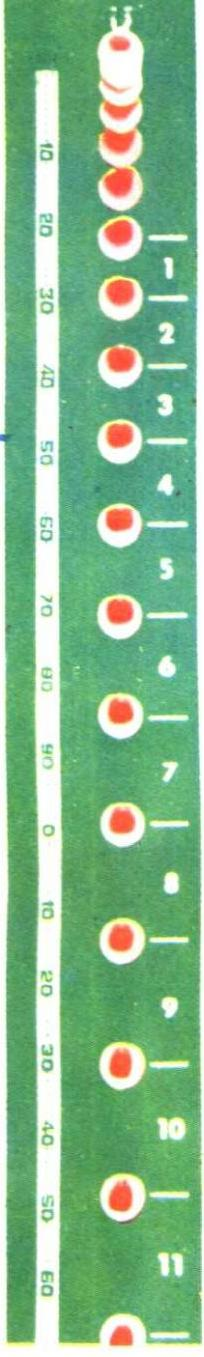
\includegraphics[max width=0.2\textwidth]{images/01912d55-147c-70aa-b0e0-1782a122f948_3_912011.jpg}
\end{center}

图 2 \_ 自由

落体的闪光

照片

\begin{center}
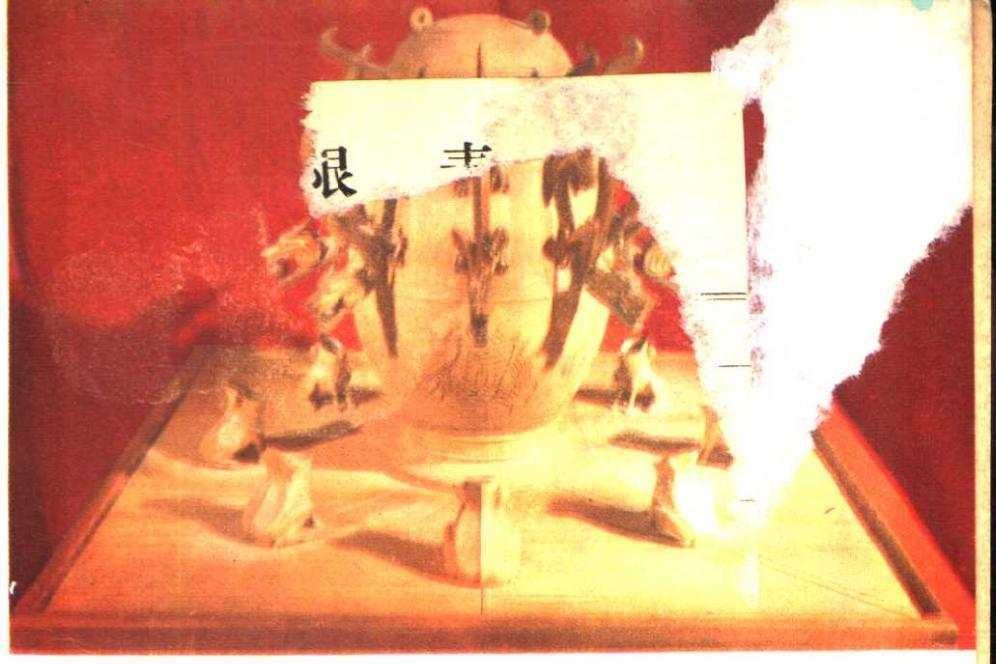
\includegraphics[max width=1.0\textwidth]{images/01912d55-147c-70aa-b0e0-1782a122f948_3_714981.jpg}
\end{center}

图 1 候风地动仪模型

\begin{center}
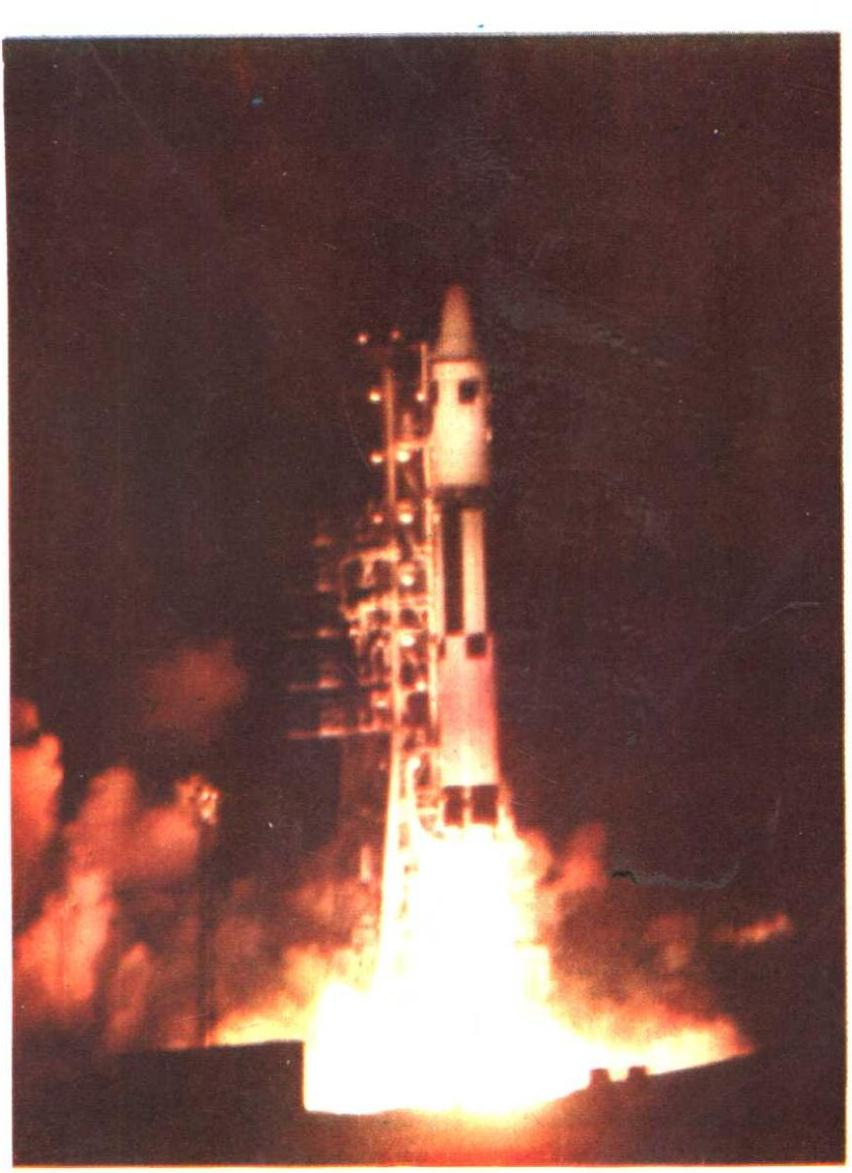
\includegraphics[max width=0.8\textwidth]{images/01912d55-147c-70aa-b0e0-1782a122f948_3_135871.jpg}
\end{center}

图 3 运载火箭点火

\begin{center}
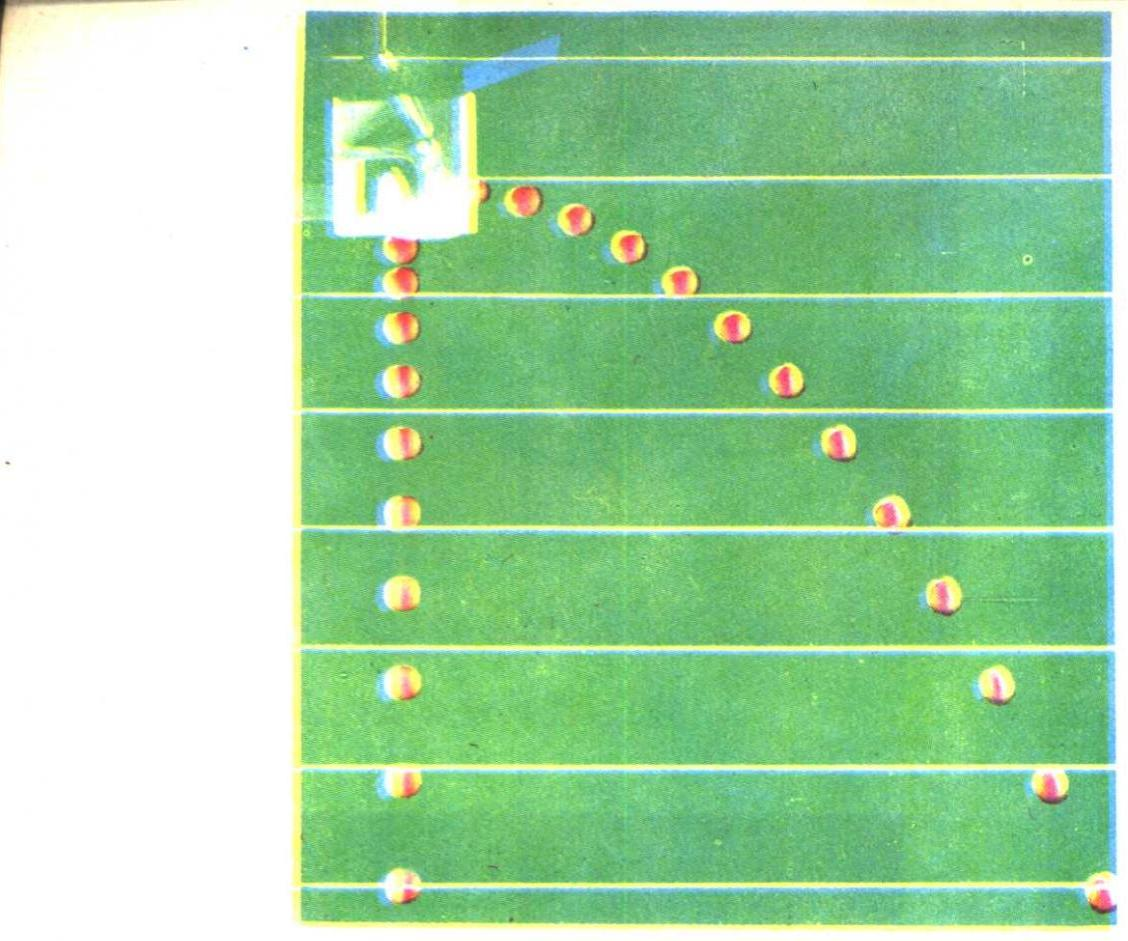
\includegraphics[max width=1.0\textwidth]{images/01912d55-147c-70aa-b0e0-1782a122f948_4_748731.jpg}
\end{center}

图 4 平抛物体的闪光照片

\begin{center}
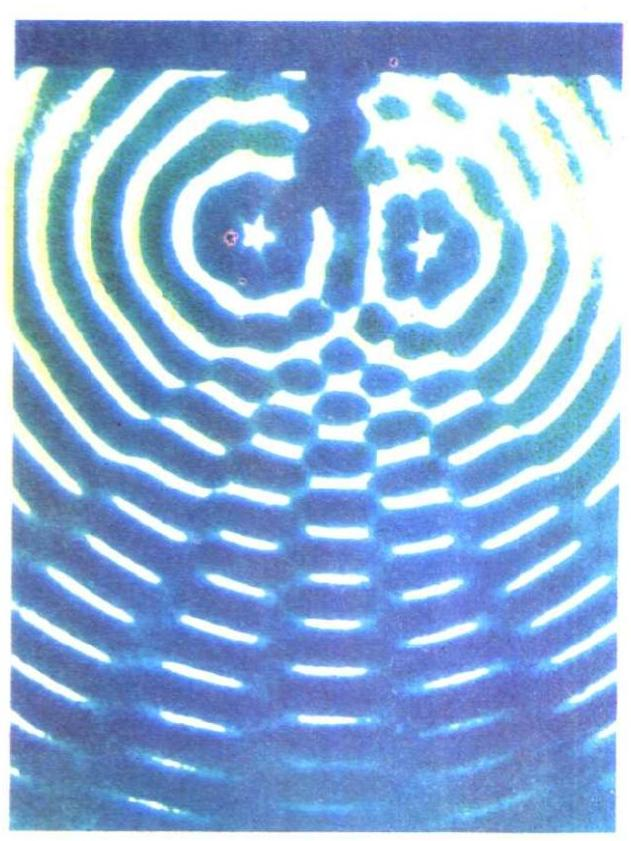
\includegraphics[max width=0.6\textwidth]{images/01912d55-147c-70aa-b0e0-1782a122f948_4_150500.jpg}
\end{center}

图 5 水波的干涉图样

\begin{center}
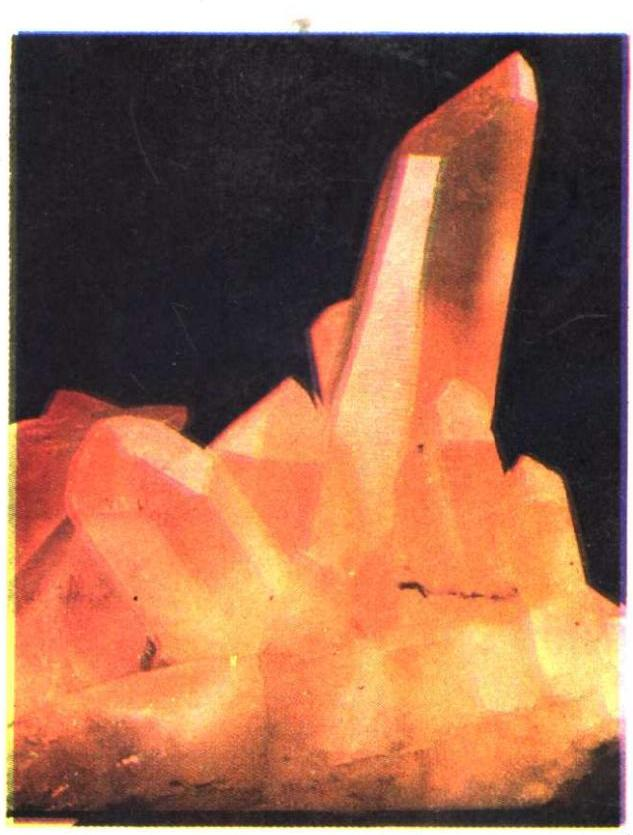
\includegraphics[max width=0.6\textwidth]{images/01912d55-147c-70aa-b0e0-1782a122f948_4_217917.jpg}
\end{center}

图 6 水晶

\section*{目 录}

绪论. 1 1

第一章 力 物体的平衡. .7

一、力 -7

二、重力 - 8

三、弹力 .11

四、摩擦力 .15

五、共点力的合成 .19

六、力的分解 .24

七、共点力作用下物体的平衡 .28

八、有固定转动轴的物体的平衡 .31

九、平衡的种类和稳度* .36

第二章 直线运动 -45

一、质点 位移和路程 .46

二、匀速直线运动 速度 .48

三、匀速直线运动的图象 .51

四、变速直线运动 平均速度 即时速度 .53

五、匀变速直线运动 加速度 .57

六、匀变速直线运动的速度 .61

七、匀变速直线运动的位移 .64

八、自由落体运动 .68

九、竖直上抛运动 .73

十、运动的合成 .75

第三章 运动和力 181

一、牛顿第一定律 -82

二、运动状态的改变 -85

三、牛顿第二定律 .87

四、质量和重量 .90

五、力学单位制 . .93

六、应用牛顿第二定律解题 .95

第四章 物体的相互作用 102

一、牛顿第三定律 102

二、动量 动量定理 .106

三、动量守恒定律 109

四、碰撞 .112

五、反冲运动及其应用 .115

第五章 曲线运动 万有引力 121

一、曲线运动 .121

二、平抛物体的运动 -124

三、斜抛物体的运动 .129

四、匀速圆周运动 .132

五、向心力和向心加速度 .134

六、应用向心力研究几个实例 138

七、离心现象* .143

八、万有引力定律 -145

九、万有引力定律在天文学上的应用* .149

十、宇宙速度 人造地球卫星* 150

第六章 机械能. 158

一、功 158

二、功率 .161

三、功和能 -163

四、动能 .165

五、做功与物体动能变化的关系 -167

六、势能 -169

七、机械能守恒定律 .171

八、应用机械能守恒定律解题 -174

第七章 机械振动和机械波. -182

一、简谐振动 -182

二、振幅、周期和频率 -185

三、单摆 187

四、简谐振动的图象 . 190

五、振动的能量 阻尼振动和受迫振动 .191

六、共振 193

七、机械波 -196

八、波的图象 - 199

九、波长、频率和波速 .200

十、波的衍射 .201

十一、波的干涉 .204

十二、声波 .207

十三、乐音 .211

十四、噪声的危害和控制 -216

十五、超声波及其应用* -218

第八章 分子运动论 热和功. -224

一、物质是由大量分子组成的 .224

二、分子的热运动 .228

三、分子间的相互作用力 .230

四、分子的动能和势能 物体的内能 .234

五、物体内能的变化 热和功 .235

六、能的转化和守恒定律 240

七、能量的利用和能源开发 -246

第九章 固体和液体的性质 -251

一、晶体和非晶体 -251

二、空间点阵 .253

三、液体的表面张力 .256

四、浸润和不浸润 -259

五、毛细现象 .261

六、熔解和凝固* -263

\begin{itemize}
\item 第十章 气体的性质. -269
\end{itemize}

\(\therefore\) 一、气体的状态和状态参量 -269

二、气体的等温变化 玻意耳-马略特定律 -273

三、气体的等容变化 查理定律 .279

四、热力学温标 .282

五、理想气体的状态方程 .285

六、气体的液化* -288

七、液体的汽化* .293

八、饱和汽和饱和汽压* .296

九、空气的湿度* .298

十、湿度计* -300

学生实验 -305

一、共点的两个力的合成 -305

二、有固定转动轴的物体的平衡 -306

三、练习使用打点计时器 -307

四、测定匀变速直线运动的加速度 -310

五、验证牛顿第二定律 -313

六、研究平抛物体的运动 -317

七、碰撞中的动量守恒 -319

八、验证向心力公式* -322

九、验证机械能守恒定律 -324

十、用冲击摆测弹丸的速度* -326

十一、用单摆测定重力加速度 -328

十二、验证玻意耳-马略 特定 律 -329

十三、验证理想气体状态方程* - 332

附录 国际单位制(SI) - 334

\section*{绪 论}

自从我们开始学习物理以来, 两年的时间已经过去了. 这段时间里, 我们学到了一些初步的物理知识, 开始懂得了科学知识在认识自然现象和了解生产技术上的重要意义. 譬如, 寒来暑往, 四时变化, 大家已经习以为常了. 但是, 冷热差别的本质又是什么呢? 以前并不清楚. 学了物理就知道了, 冷热程度跟分子运动的快慢有关系. 物体的分子运动得越快, 物体就越热; 反之就越冷. 又如, 电灯为什么会亮呢? 学习物理之前也说不清楚. 学了物理就明白了, 原来是电流在灯丝里做功, 使电能转化成光能. 电流又是什么呢? 是电子的定向移动. 这样, 学了物理, 我们对周围世界的认识, 比学习物理以前就要深刻得多了.

我们在初中学过的物理知识, 还是很浅易的. 例如, 我们虽然学过了力, 知道力是改变物体运动状态的原因, 但是力究竟是怎样改变物体运动状态的呢? 力的大小跟物体运动状态的变化有什么定量的关系呢? 这些问题我们都还没有研究. 我们学过了闭合电路的一部分做切割磁力线的运动时电路中要产生感生电流, 但是感生电流的大小又是怎样确定的呢? 我们也还没有进一步讨论过. 还有一些重要的物理知识, 我们在初中还没有学到. 例如, 光的本质到底是什么, 常常听说的原子能到底是怎么回事, 等等. 为了扩大和加深对世界的认识, 我们还需要进一步学习物理学.

我们进一步学习物理学的目的, 并不只是为了认识世界, 更重要的还在于改造世界, 学了物理知识要为祖国的社会主义建设事业服务. 我们知道, 物理学作为一门独立的学科, 是在十七世纪以后才形成的. 自那以后, 物理学的发展十分迅速, 对于整个科学技术的进步, 起了巨大的作用. 特别是十九世纪以来, 科学技术上每一次重大的突破, 都是跟物理学的进展分不开的. 如果不是在十九世纪中期发现了电磁感应现象, 建立起相应的电磁理论, 就不会有发电机、电动机, 现代的电力化生产就不可能实现. 今天, 广泛应用于飞机、汽车、坦克、 拖拉机、机车、轮船等的内燃机, 也是在十九世纪深入研究了气体的性质和热学理论的基础上发展起来的. 进入二十世纪, 物理学更广泛地应用于工农业生产和科学技术的各个领域, 成为科学技术的重要基础. 影响深远的原子能和电子技术的发展, 都是从物理学上的重大发现开端的. 可以说, 生产的发展推动了科学技术的进步, 科学技术的进步反过来又推动了生产的发展, 改变了生产的面貌. 所以, 为了适应我国工业、 农业、国防和科学技术现代化的需要, 我们很需要进一步学习物理知识.

怎样才能进一步学好物理呢?

\section*{一、认真阅读课本}

课本里讲的是前人长期积累下来的最基础的知识, 要理解并能运用这些知识, 首先就要认真阅读课本. 人们在长期的科学研究中积累下来的物理知识, 我们是可以学懂的, 要有这个信心. 但物理知识跟其他科学知识一样, 也不是一看就懂、 一学就会的, 所以对物理课本我们要反复阅读, 深入思考, 这才算是认真阅读课本. 有一些同学认为, 学物理主要是做习题, 这是一种误解. 做习题也是学好物理知识的重要环节. 但是做习题的目的是巩固知识, 加深对知识的理解, 并学会运用它们. 忽视了对基本的概念和定律的理解而去盲目地做题目, 是收不到应有效果的.

认真阅读课本, 还可以培养和提高自学能力. 有了自学能力, 就可以通过课外阅读, 学到课本里没有学到的东西, 知识就丰富了, 眼界也开阔了. 这对于活跃我们的思想, 提高我们的科学思维能力, 是大有好处的. 还应该看到, 学校生活毕竟是短暂的. 未来不论我们从事哪种工作, 都需要在工作中不断提高文化科学水平, 这种提高主要靠自学, 即自己阅读有关书籍和报刊. 在学校里通过认真阅读课本培养起来的这种自学能力, 对自己将来的发展将是十分重要的.

阅读课本, 除了学习物理知识之外, 还要注意学习物理学中研究问题的方法. 例如, 研究物体的运动, 从匀速直线运动开始, 再一步步研究非匀速的运动和曲线运动. 这就是先从最简单的、便于研究的情况入手, 层层深入, 逐步揭示出比较复杂的规律. 研究力和运动的关系, 要先考虑物体完全不受外力作用的特殊情况, 得出惯性定律, 然后再研究物体受力后运动状态如何变化, 一步一步地深入揭露出力学的基本规律. 在课本里, 研究问题的方法是在研究解决各个物理问题的过程中体现出来的. 一些典型的、常用的方法, 在书中多次反复出现. 阅读课本时应该多留心、多揣摩, 逐步加深对研究方法的领会.

你们的老师将在教学中告诉你们许多有效地阅读物理课本的方法, 你们自己在认真阅读中也将不断积累经验, 越来越会从读书中获得知识.

\section*{二、认真听讲}

我们在自己的物理知识还不多的时候, 要学好物理知识, 掌握研究方法, 发展自己的能力, 都离不开老师的传授和指导. 在课堂上, 老师系统地讲解物理概念和定律, 指导我们做实验, 组织我们讨论探索新知识, 纠正我们常犯的错误, 解答我们的疑难, 指明学习的重点, 还经常点拨思路, 在科学方法的运用上做出良好示范. 因此, 认真听课是我们学习中少走弯路, 顺利学好物理的保证.

在听课中, 也跟阅读时一样, 不只要弄清基本知识, 还要学习解决物理问题的思路和方法. 从某种意义上讲, 提高思维能力, 掌握研究问题的科学方法, 比掌握知识更要紧. 能力提高了, 善于思考和研究问题, 就能灵活运用学过的知识去解决各种实际问题, 这正是我们学习的目的所在. 因此, 在听课时, 不要只是消极地接受老师讲授的知识, 重要的是要认真开动脑筋, 积极思维, 把精力集中在理解上而不是在记忆上. 假使有的问题一时没有搞懂, 要尽可能用看书学习、观察实验等方法来自己搞懂它, 只有必要时再向老师请教. 老师在课堂上可能会组织我们进行讨论, 这时要认真参加, 勇于发表自己的看法, 培养与别人科学地交换意见、讨论问题的能力.

\section*{三、注意观察, 做好实验}

物理知识跟其他各科知识一样, 都是从实践中发源的. 想想看, 如果不研究反射光线跟入射光线的关系, 能发现光的反射定律吗? 不研究电流使磁针偏转的现象, 能认识电流周围存在着磁场吗? 我们学习物理知识, 跟前人探索物理知识的过程, 有很多相似之处. 认真观察自然现象, 自己动手做实验, 有助于我们形成正确的概念, 加深对物理定律的理解. 我们在初中虽然做过一些物理实验, 但初中物理实验一般都比较简单, 受到的基本训练还是不充分的. 到了高中, 我们应该继续重视实验, 在老师的指导下, 学到更多的做好实验的本领, 给物理知识的学习打下坚实的基础.

为了做好实验, 在每次实验之前, 一定要明确实验的目的, 弄懂它的原理, 了解所用仪器的性能, 搞清实验的步骤. 在实验中要遵守操作规程, 认真观察现象, 仔细记录必要的数据. 实验后要对所得的数据进行分析, 作出合理的结论, 必要时还要进一步研究某些不够清楚的问题.

除了自己动手做好实验之外, 对老师做的演示实验, 也要注意观察, 分析实验现象, 得出应有的结论, 还要努力创造条件, 在课外多做一些简单的小实验. 在日常生活中, 也要留心观察各种物理现象, 用我们学过的物理知识进行分析研究. 这也是理论联系实际、提高思维能力的一种好方法.

总之, 只要我们多观察、多动手, 又能开动脑筋、认真读书、认真听讲, 辅之以必要的练习, 学好物理知识是可以做到的.

\section*{第一章 力 物体的平衡}

\section*{一、力}

我们在初中学过, 力是物体对物体的作用. 人推车, 人对车施加了力. 马拉犁, 马对犁施加了力. 机车牵引列车, 机车对列车施加了力. 绳子吊起货物, 绳子对货物施加了力. 磁铁吸引铁块, 磁铁对铁块施加了力. 可见, 力是物体对物体的作用. 一个物体受到力的作用, 一定有另一个物体对它施加这种作用. 力是不能离开施力和受力物体而独立存在的.

我们还学过, 力是有大小的, 力的大小可以用弹簧秤测量. 在国际单位制中, 力的单位是牛顿, 简称为牛, 国际符号是 \(\mathrm{N}\) . 日常生活和生产中常用的力的单位是千克力. 千克力和牛顿的关系是

\[
\text{1 千克力} = {9.8}\text{牛.}
\]

力不仅有大小, 而且有方向. 树上的苹果受到的重力是向下的. 水里的船舶受到的浮力是向上的. 马对车的拉力是向前的, 地对犁的阻力是向后的.

既有大小、又有方向的力, 可以用一根带箭头的线段来表示. 线段的长短表示力的大小, 箭头的指向表示力的方向, 箭尾常常画在力的作用点上. 这种表示力的方法, 叫做力的图示.

例如,卡车对拖车的牵引力 \(F\) 的大小是 2000 牛,方向是水平向右,做 \(F\) 的图示时,可以照图 1-1 甲那样,先选定一个

\begin{center}
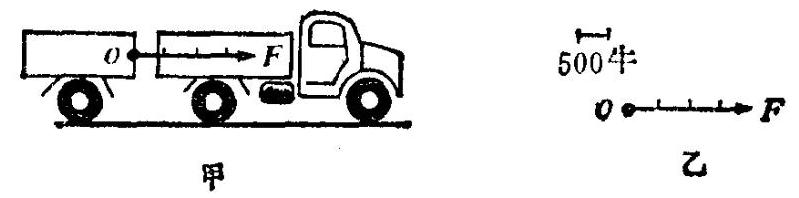
\includegraphics[max width=0.8\textwidth]{images/01912d55-147c-70aa-b0e0-1782a122f948_17_361745.jpg}
\end{center}

图 1-1

标度,这里是选定 3 毫米长的线段表示 500 牛的力,再从 \(\mathbf{F}\) 的作用点 \(O\) 向右水平地画一段四倍于标度 (12 毫米) 的线段,然后加上向右的箭头就行了. 为了简便, 也可以照图 1-1 乙那样,不画出车,而用点 \(O\) 表示拖车,做出力 \(F\) 的图示.

\section*{二、重 力}

自从我们学习物理以来, 见到过的力的名称已经不少了. 它们可以分为两类. 一类是根据力的性质来命名的, 如重力、 弹力、摩擦力、分子力、电力、磁力, 等等; 另一类是根据力的效果来命名的, 如拉力、压力、支持力、动力、阻力, 等等. 根据效果命名的不同名称的力, 性质可能相同. 例如, 绳子的拉力、 车轮的压力、路面的支持力实际上都是弹力, 只是作用的效果不同. 根据效果命名的同一名称的力, 性质可能不同. 例如, 货物被绳吊起时的动力是绳的弹力, 重物落下时的动力是重力. 不论什么性质的力, 只要它的效果是加快物体运动的, 就可以叫做动力; 是阻碍物体运动的, 就可以叫做阻力. 以后, 我们还会遇到根据力的效果来命名的其他的力.

从力的性质来看, 力学中经常遇到的有重力、弹力和摩擦力. 从这一节起, 分别讨论这几种力. 这里先讲重力.

地球上的一切物体, 都受到地球的吸引, 物体受到的重力就是由于地球的吸引而产生的. 重力有时也叫重量. 重力的方向总是竖直向下的.

重力的大小可以用弹簧秤称出 (图 1-2). 这时物体对弹簧秤的拉力 (图甲) 或压力 (图乙) 等于物体受到的重力. 如果不用弹簧秤, 而是把物体挂在绳上或放在水平支持物上, 在静止的情况下, 物体对竖直悬绳的拉力或对水平支持物的压力, 也等于物体受到的重力.

\begin{center}
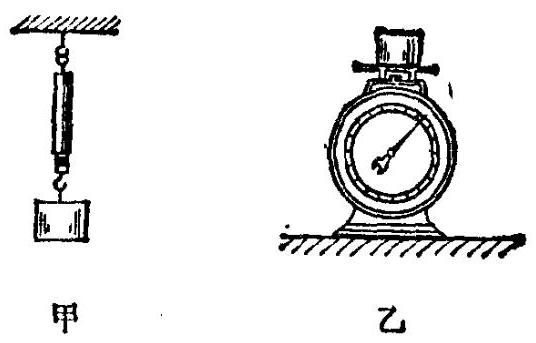
\includegraphics[max width=0.6\textwidth]{images/01912d55-147c-70aa-b0e0-1782a122f948_18_560108.jpg}
\end{center}

图 1-2 弹簧秤

在已知物体质量的情况下, 重力的大小可以根据初中学过的重力 \(G\) 跟质量 \(m\) 成正比的关系式 \(G = {mg}\) 计算出来,式中 \(g = {9.8}\) 牛/千克,表示质量是 1 千克的物体受到的重力是 9.8 牛.

物体的各个部分都受重力的作用. 但是, 我们可以认为各部分受到的重力作用都集中于一点, 这个点就是重力的作用点, 叫做物体的重心.

薄板形物体的重心, 可以用悬挂法来确定. 如图1-3所示,

\begin{center}
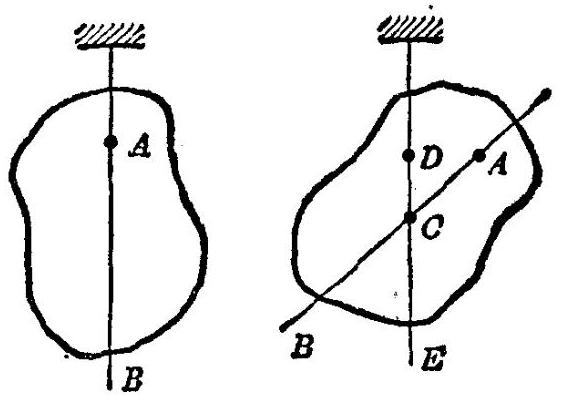
\includegraphics[max width=0.6\textwidth]{images/01912d55-147c-70aa-b0e0-1782a122f948_19_608135.jpg}
\end{center}

图 1-3

先在 \(A\) 点把薄板悬挂起来. 这时薄板只受两个力的作用: 重力和悬绳的拉力. 在初中我们学过, 只受两个力作用的物体, 如果保持静止或匀速直线运动状态, 这两个力一定作用在同一条直线上, 大小相等, 方向相反. 因此, 当薄板处于静止状态时, 它所受的重力必定跟悬绳对它的拉力在同一竖直线上, 所以它的重心一定在通过 \(A\) 点的竖直线 \({AB}\) 上. 然后,再在 \(D\) 点把薄板悬挂起来,同样可以知道,薄板的重心一定在通过 \(D\) 点的竖直线 \({DE}\) 上. \({AB}\) 和 \({DE}\) 的交点 \(C\) 就是薄板的重心.

质量分布均匀的物体, 重心的位置只跟物体的形状有关. 如果物体的形状是中心对称的, 对称中心就是物体的重心. 例如, 均匀圆板的重心在圆心, 均匀直棒的重心在它的中点, 均匀球体的重心在球心,均匀圆柱体的重心在轴线的中点,等等.

质量分布不均匀的物体, 重心的位置除跟物体的形状有关外, 还跟物体质量的分布情况有关. 例如, 载重汽车的重心, 随着所装货物的重量和装载位置而变化; 起重机的重心, 随着提升重物的重量和高度而变化.

\section*{练习 -}

(1)请你画出下面几个力的图示, 并说明施力物体和受力物体.

① 机车对列车水平向右的牵引力 \({1.5} \times {10}^{5}\) 牛.

② 悬绳对重物竖直向上的拉力 50 牛.

③ 铁锤对钉子竖直向下的打击力 250 牛。

④ 质量是 5 千克的物体受到的重力.

(2)请你画出下面几个力的图示:

① 重量是 5 牛的静止物体对竖直悬绳的拉力.

② 重量是 1 牛的茶杯对水平桌面的压力.

(3)找一块薄板, 用悬挂法求出它的重心位置. 以这个重心位置作支持点, 用手指尖把薄板支撑起来, 薄板会不会水平静止? 为什么?

\section*{三、弹 力}

竹竿受力可以变弯, 弹簧受力可以伸长或缩短. 象这样, 物体在力的作用下发生的形状改变叫做形变.

物体在力的作用下发生的形变, 有的明显, 能够直接看到; 有的很不明显, 不能直接看到, 只有想点特殊的方法才能察觉. 例如, 用手按压玻璃瓶时, 我们看不到玻璃瓶的形变. 但是, 用手按压图 1-4 中装满水的玻璃瓶时, 细管中的水面就上升, 松开手时, 管中的水面又降回原处. 这样我们就察觉到, 瓶子在受到按压时发生了形变.

图 1-4 的实验还表明: 在手的压力下发生形变的瓶子, 除去压力以后又恢复原状. 在力的作用下发生形变的物体, 在除去外力后能够恢复原状的性质, 叫做弹性. 在外力停止作用后, 能够恢复原状的形变叫做弹性形变.

\begin{center}
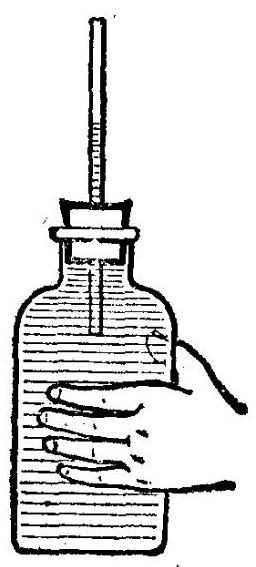
\includegraphics[max width=0.3\textwidth]{images/01912d55-147c-70aa-b0e0-1782a122f948_21_435685.jpg}
\end{center}

图 1-4

被压缩或拉伸的弹簧, 可以使跟它接触的小车受到力的作用, 开始运动 (图 1-5). 拿一根

\begin{center}
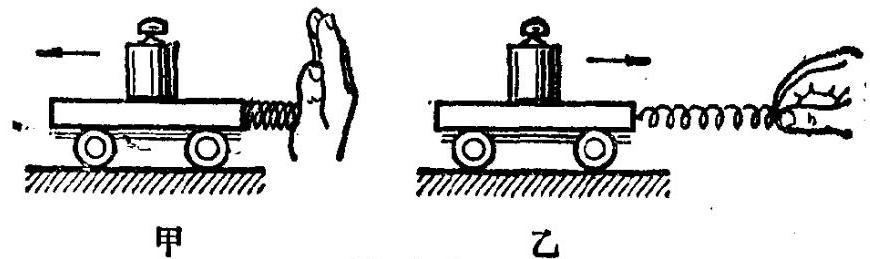
\includegraphics[max width=0.9\textwidth]{images/01912d55-147c-70aa-b0e0-1782a122f948_21_521571.jpg}
\end{center}

图 1-5

细竹竿拨动水中的木头, 竹竿变弯了, 同时木头受到竹竿的作用力, 开始移动 (图 1-6). 可见, 发生弹性形变的物体, 由于要恢复原状, 会对跟它接触的物体产生力的作用. 这种力叫做弹力.

\begin{center}
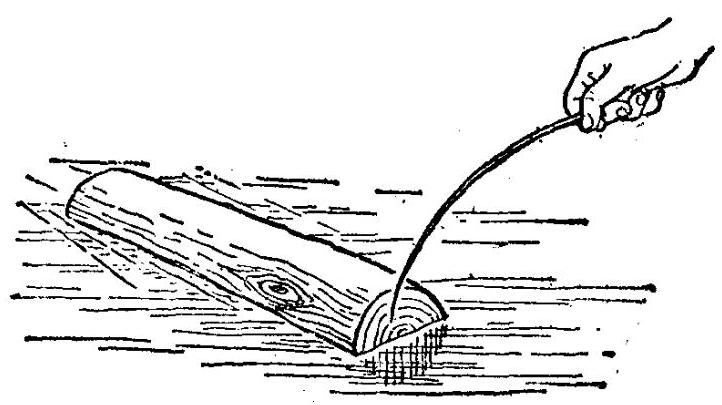
\includegraphics[max width=0.8\textwidth]{images/01912d55-147c-70aa-b0e0-1782a122f948_21_487951.jpg}
\end{center}

图 1-6

弹力产生在直接接触而发生弹性形变的物体之间.

放在水平桌面上的书, 在重力作用下与桌面互相接触, 使书和桌面同时发生微小的形变. 书由于发生微小的形变, 而对桌面产生垂直于桌面向下的弹力, 这就是书对桌面的压力 (图 1-7 左). 桌面由于发生微小的形变, 而对书产生垂直于书面向上的弹力, 这就是桌面对书的支持力 (图 1-7 右).

\begin{center}
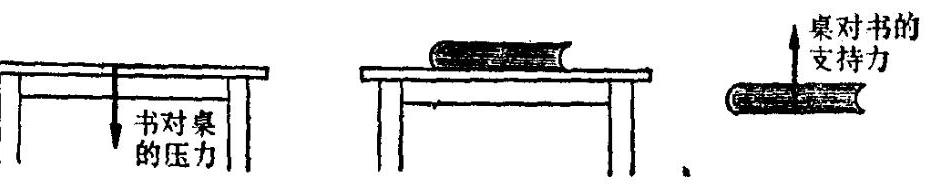
\includegraphics[max width=1.0\textwidth]{images/01912d55-147c-70aa-b0e0-1782a122f948_22_890095.jpg}
\end{center}

图 1-7

可见, 通常所说的压力和支持力都是弹力. 压力是物体对支持物的弹力, 方向总是垂直于支持面而指向支持物. 支持力是支持物对被支持的物体的弹力, 方向总是垂直于支持面而指向被支持的物体.

挂在电线下面的电灯, 在重力作用下拉紧电线, 使电灯和电线同时发生微小的形变. 电灯由于发生微小的形变, 而对电线产生向下的弹力, 这就是电灯对电线的拉力 (图 1-8 左).

\begin{center}
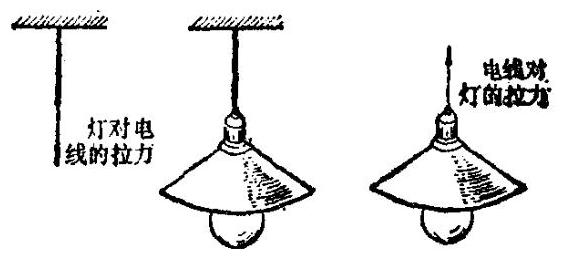
\includegraphics[max width=0.6\textwidth]{images/01912d55-147c-70aa-b0e0-1782a122f948_22_129010.jpg}
\end{center}

图 1-8

电线由于发生微小的形变, 而对电灯产生向上的弹力, 这就是电线对电灯的拉力(图 1-8 右).

可见, 通常所说的拉力也是弹力. 绳的拉力是绳对所拉物体的弹力, 方向总是沿着绳而指向绳收缩的方向.

弹力和形变的关系, 一般来讲比较复杂. 而弹簧的弹力和形变 (伸长或缩短) 的关系比较简单. 实验表明, 弹簧发生弹性形变时,弹力的大小 \(f\) 跟弹簧伸长 (或缩短) 的长度 \(x\) 成正比, 即

\[
f = {kx}\text{.}
\]

式中的 \(k\) 称为弹簧的倔强系数,不同弹簧的倔强系数一般是不同的. 这个规律是英国科学家胡克发现的, 叫做胡克定律.

\section*{练习二}

(1) 放在水平桌面上的书, 对桌面的压力等于它的重量. 能不能说书对桌面的压力就是它的重量? 为什么?

(2)有四位同学把斜面对重物的支持力 3 牛, 分别画成图 1-9 中的四种样子, 你说哪个图画得对?

\begin{center}
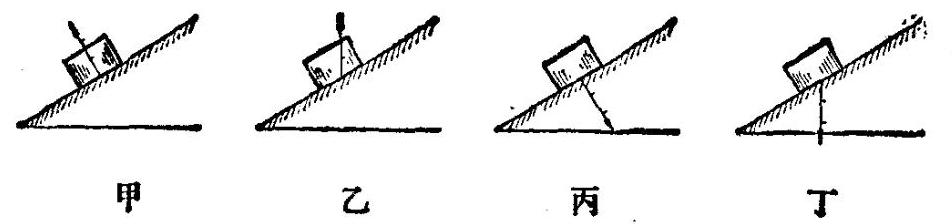
\includegraphics[max width=1.0\textwidth]{images/01912d55-147c-70aa-b0e0-1782a122f948_23_648673.jpg}
\end{center}

图 1-9

(3)如图 1-10 所示, 用两根绳子把一个物体挂在天花板上, 这个物体受到几个力的作用? 指出施力物体, 并把力的方向表示出来。

\begin{center}
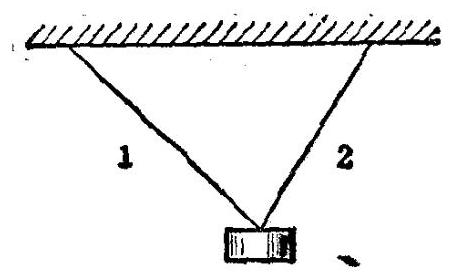
\includegraphics[max width=0.5\textwidth]{images/01912d55-147c-70aa-b0e0-1782a122f948_24_372526.jpg}
\end{center}

图 1-10

(4)在水平桌面上的两个球, 靠在一起但并不互相挤压, 它们之间有相互作用的弹力吗? 为什么?

\section*{四、摩 擦 力}

静摩擦力 如图 1-11 所示, 放在桌面上的木块跟跨过滑

\begin{center}
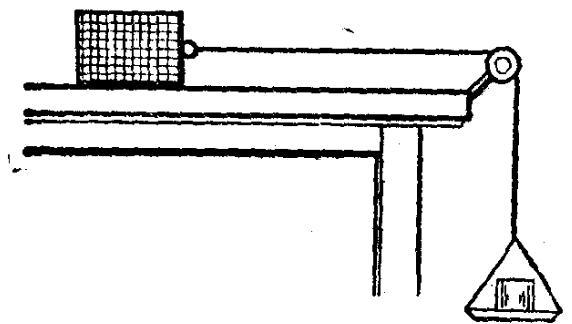
\includegraphics[max width=0.6\textwidth]{images/01912d55-147c-70aa-b0e0-1782a122f948_24_859189.jpg}
\end{center}

图 1-11

轮的绳子相连接, 绳子的另一端悬挂吊盘, 盘上有重物. 木块在绳子的拉力作用下会运动起来. 但是, 当重物的重量比较小时, 木块静止不动. 这表明木块除了受到绳子的拉力外, 还受到一个与拉力大小相等、方向相反的力, 它起着阻碍木块运动的作用. 这个力就是木块和桌面之间的摩擦力. 摩擦力也是作用在相互接触的两个物体之间的力. 上面讲的摩擦力, 发生在两个相对静止的物体之间, 所以叫做静摩擦力.

静摩擦力是很常见的. 例如, 拿在手中的瓶子、毛笔不会滑落, 就是静摩擦力作用的结果. 静摩擦在生产技术中的应用是很多的. 例如, 皮带运输机(图 1-12) 是靠货物和传送皮带之间的静摩擦力, 把货物送往别处的. 皮带传动 (图1-13) 是靠皮带和皮带轮间的静摩擦力, 来传递动力的.

\begin{center}
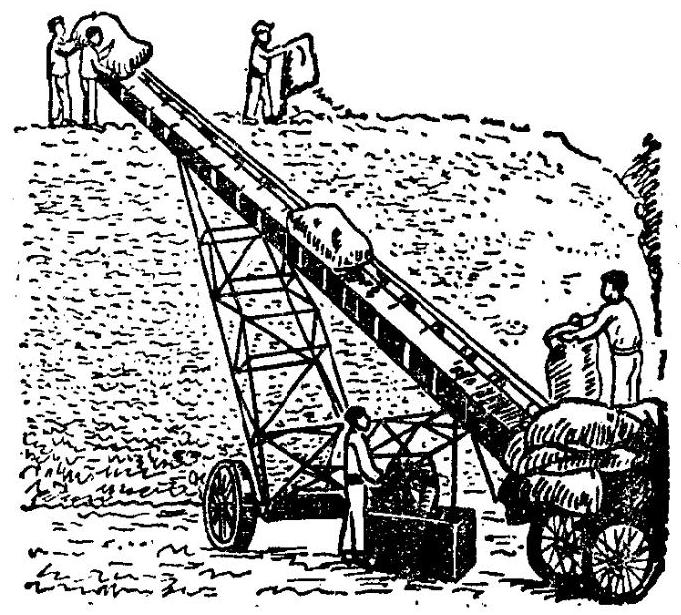
\includegraphics[max width=0.7\textwidth]{images/01912d55-147c-70aa-b0e0-1782a122f948_25_316673.jpg}
\end{center}

图 1-12 皮带运输机

\begin{center}
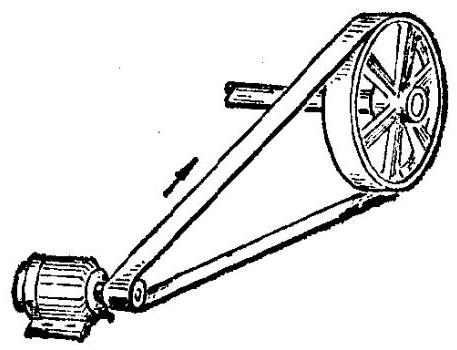
\includegraphics[max width=0.5\textwidth]{images/01912d55-147c-70aa-b0e0-1782a122f948_25_374012.jpg}
\end{center}

图 1-13 皮带传动

在图 1-11 的吊盘上继续加重物, 使木块受到的拉力增大. 如果重物的重量还不够重, 木块仍然保持静止. 可见, 静摩擦力随着拉力的增大而增大. 但是, 当吊盘上的重物增加到某一重量时, 木块就会开始沿着桌面滑动, 这表明静摩擦力有一个最大值. 静摩擦力的最大值叫做最大静摩擦力.

滑动摩擦力 木块开始滑动后, 仍然需要一个拉力才能维持匀速运动, 否则它就会逐渐停下来. 这表明滑动的物体也受到摩擦力的阻碍. 滑动物体受到的摩擦力叫做滑动摩擦力. 滑动摩擦力的方向总是阻碍物体运动的.

滑动摩擦力的大小与哪些因素有关呢?

为了研究这个问题. 我们调整图 1-11 中吊盘上重物的重量, 使我们只要沿着拉力的方向轻轻推一下木块, 木块就能在桌面上做匀速运动. 这时绳子对木块的拉力就等于木块与桌面间的滑动摩擦力. 它的大小跟吊盘与重物的总重量相等.

现在, 我们在木块上加一个重物, 增大木块和桌面之间的压力, 可以看到木块与桌面之间的滑动摩擦力也增大了.

大量的实验表明: 两个物体间的滑动摩擦力的大小 \(f\) 跟这两个物体表面间的压力的大小 \(N\) 成正比,即

\[
\frac{f}{N} = \mu \text{ 或 }f = {\mu N}.
\]

式中的 \(\mu\) ① 称为滑动摩擦系数,它的数值既跟相互接触的两个物体的材料有关, 又跟接触面的情况 (如粗糙程度等) 有关. 在相同的压力下, 滑动摩擦系数越大, 滑动摩擦力就越大. 滑动摩擦系数是两个力的比值, 没有单位.

① \(\mu\) : 希腊字母,汉语拼音读法是 \({\mathrm{{miu}}}_{2}\)

几种材料间的滑动摩擦系数

\begin{center}
\adjustbox{max width=\textwidth}{
\begin{tabular}{|c|c|}
\hline
材 料 & 滑动摩擦系数 \\
\hline
钢一钢 & 0.25 \\
\hline
木一木 & 0.30 \\
\hline
木一金属 & 0.20 \\
\hline
皮革一铸铁 & 0.28 \\
\hline
钢一冰 & 0.02 \\
\hline
木头一冰 & 0.03 \\
\hline
橡皮轮胎一路面(干) & 0.71 \\
\hline
\end{tabular}
}
\end{center}

〔例题] 在东北的林场中, 冬季常用马拉的雪橇运木材, 雪橇有两个与冰面接触的钢制滑板. 如果冰面是水平的, 雪橇和所装的木材的总质量是 5.0 吨, 滑板与冰面间的滑动摩擦系数是 0.027 , 马要在水平方向上用多大的力才能拉着雪橇在冰道上匀速前进?

要使雪橇匀速前进, 马的拉力应该跟滑动摩擦力大小相等. 所以求出滑动摩擦力, 就知道了马的拉力. 滑动摩擦力可以用公式 \(f = {\mu N}\) 求出. 雪橇对水平冰面的压力 \(N\) 等于雪橇和所装木材的重量 \(G\) ,可以根据它们的总质量 \(m\) 用公式 \(G\) \(= {mg}\) 算出.

解: \(\mu = {0.027}\) ,

\[
N = G = {mg} = {5.0} \times {10}^{3}\text{千克} \times {9.8}\text{牛/千克}
\]

\[
= {4.9} \times {10}^{4}\text{ 牛,}
\]

\[
f = {\mu N} = {0.027} \times {4.9} \times {10}^{4}\text{ 牛 }
\]

\[
= {1.3} \times {10}^{3}\text{ 牛. }
\]

所以,马要在水平方向上用 \({1.3} \times {10}^{3}\) 牛的拉力.

\section*{练习 \(\equiv\)}

(1)手压桌面向前移动, 会明显地感到有阻力阻碍手的移动. 手对桌面的压力越大, 会感到阻力越大. 试一试, 说明这是为什么?

(2)放在斜面上的砖 (图 1-14 甲), 受到三个力的作用(图 1-14乙). 请你说出各力的名称和施力物体.

\begin{center}
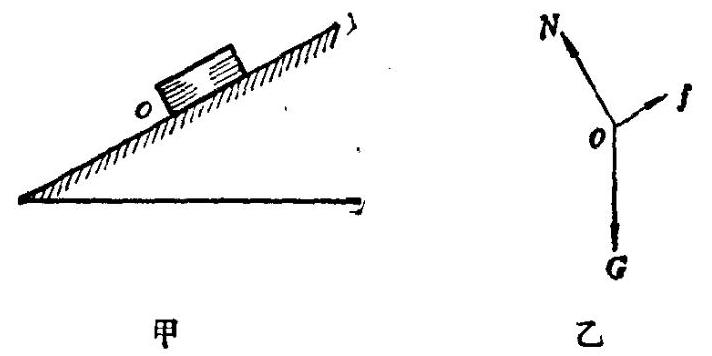
\includegraphics[max width=0.7\textwidth]{images/01912d55-147c-70aa-b0e0-1782a122f948_28_563798.jpg}
\end{center}

图 1-14

(3)要在木桌上测重量是 12.0 牛的木块的滑动摩擦力, 用量程是 10.0 牛的弹簧秤可以吗?

(4)如果你用 20 牛的水平推力, 使一块重量是 40 牛的砖在水平地面上匀速滑动, 你能求出砖和地面之间的滑动摩擦系数吗?

(5)请你设计一个测量纸跟桌面之间滑动摩擦系数的方法. 如果有条件的话, 请你实际测一测.

\section*{五、共点力的合成}

一件行李可以由几个人一起提, 也可以由一个人来提. 一辆拖车可以由几匹马一起拉, 也可以由一部拖拉机来拉. 这说明一个力常常可以跟几个力共同作用达到相同的效果.

如果一个力作用在物体上, 它产生的效果跟几个力共同作用的效果相同, 这个力就叫做那几个力的合力, 而那几个力就叫做这个力的分力. 求几个已知力的合力叫做力的合成, 求一个已知力的分力叫做力的分解.

物体同时受几个力的作用, 如果这几个力都作用在物体的同一点,或者它们的作用线 \({}^{\left( 1\right) }\) 相交于同一点,这几个力就叫做共点力.

让我们通过实验来研究两个互成角度的共点力的合成.

我们可以象图 1-15 甲那样,用两条线绳把重物 \(G\) 悬挂起

\begin{center}
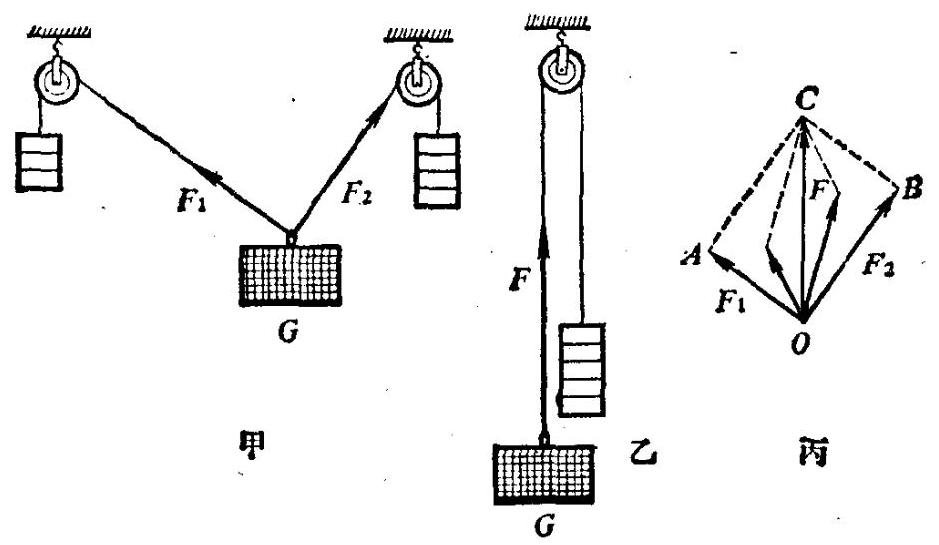
\includegraphics[max width=1.0\textwidth]{images/01912d55-147c-70aa-b0e0-1782a122f948_29_288002.jpg}
\end{center}

图 1-15

来. 也可以象图 1-15 乙那样,用一条线绳把重物 \(G\) 悬挂起来. 显然,两条线绳对重物的拉力 \({F}_{1}\text{、}{F}_{2}\) ,与一条线绳对重物的拉力 \(F\) 的作用效果相同. 所以, \({F}_{1}\text{、}{F}_{2}\) 是 \(F\) 的分力, \(F\) 是 \({F}_{1}\) 、 \({F}_{2}\) 的合力. 那么,合力 \(F\) 的大小和方向跟分力 \({F}_{1}\text{、}{F}_{2}\) 的大小和方向之间有什么关系呢?

\customfootnote{

① 在初中学过, 通过力的作用点沿力的方向所引的直线, 叫做力的作用线.

}

用一点 \(O\) 代表重物 \(G\) ,从 \(O\) 点分别画出代表分力 \({F}_{1}\text{、}{F}_{2}\) 和合力 \(F\) 的线段 \({OA}\text{、}{OB}\) 和 \({OC}\) ,作 \({F}_{1}\text{、}{F}_{2}\) 和 \(F\) 的端点的联线 \({AC}\) 和 \({BC}\) . 我们发现,四边形 \({OACB}\) 是一个平行四边形,代表合力 \(F\) 的有向线段 \({OC}\) 就是平行四边形的对角线 (图 1-15 丙). 改变 \({F}_{1}\) 和 \({F}_{2}\) 的方向和大小,发现合力 \(F\) 总是以分力 \({F}_{1}\text{、}{F}_{2}\) 为邻边的平行四边形的对角线.

由此可见, 求两个互成角度的共点力的合力, 可以用表示这两个力的线段作邻边, 作平行四边形, 它的对角线就表示合力的大小和方向. 这叫做力的平行四边形法则.

当共点的两个分力在同一直线上时, 合力怎样呢?

如果这两个分力方向相同, 例如甲乙两位同学, 同学甲用 \({\mathbf{F}}_{1} = {200}\) 牛的力向东拉车,同学乙 用 \({\mathbf{F}}_{2} = {100}\) 牛的力向东推车,那么合力就是 \(F = {300}\) 牛,方向也向东,即合力的大小等于两个分力的大小之和, 合力的方向与两个分力的方向相同(图 1-16 甲).

\begin{center}
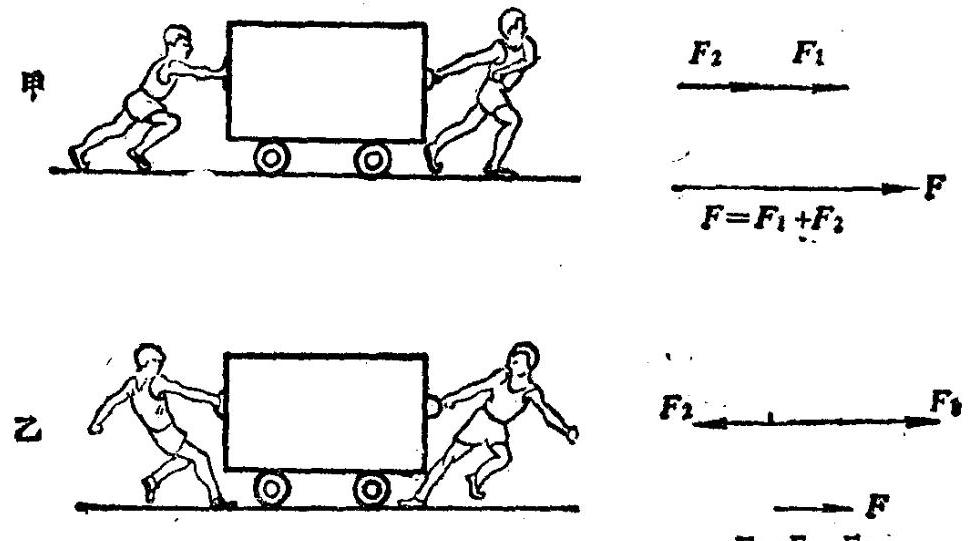
\includegraphics[max width=1.0\textwidth]{images/01912d55-147c-70aa-b0e0-1782a122f948_30_993254.jpg}
\end{center}

图 1-16

如果这两个分力方向相反,例如,同学甲仍用 \({F}_{1} = {200}\) 牛的力向东拉,而同学乙却用 \({F}_{2} = {100}\) 牛的力向西拉. 那么合力就是 \(F = {100}\) 牛,方向与同学甲的拉力相同,也向东,即合力的大小等于两个分力的大小之差, 合力的方向与分力中数值大的那个分力的方向相同 (图 1-16 乙).

两个以上的共点力的合力, 也可以用平行四边形法则求出来, 步骤是: 先求出任意两个力的合力, 再求这个合力与第三个力的合力, 依此类推, 直到求出所有共点力的合力为止. 图 1-17 中的 \(F\) 就是力 \({F}_{1}\text{、}{F}_{2}\text{、}{F}_{3}\) 的合力.

\begin{center}
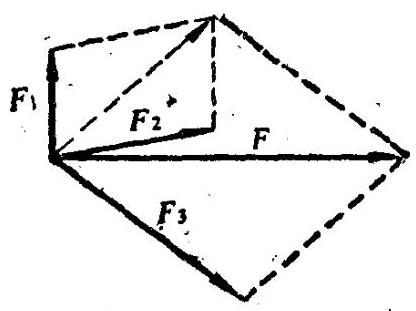
\includegraphics[max width=0.4\textwidth]{images/01912d55-147c-70aa-b0e0-1782a122f948_31_250501.jpg}
\end{center}

图 1-17

在物理学中, 象力这样既要由大小, 又要由方向来确定的物理量叫做矢量. 而象长度、质量、时间那样的只有大小没有方向的物理量叫做标量. 平行四边形法则是矢量合成的普遍法则, 对于任何矢量的合成都适用.

〔例题〕两个小孩拉一辆车子, 一个小孩用的力是 45 牛, 另一个小孩用的力是 60 牛,这两个力的夹角是 \({90}^{ \circ }\) . 求他们的合力.

这是一个已知分力求合力的问题, 可以用作图法求出. 先选一个标度,并用一点 \(O\) 代表小车,作两个拉力 \({F}_{1}\text{、}{F}_{2}\) 的图示. 由于题中没有明确给出拉力的具体方向, 所以可以选择我们便于作图的任何方向作 \({F}_{1}\text{、}{F}_{2}\) 的图示,只要保持它们的夹角是 \({90}^{ \circ }\) 就行了. 然后,以 \({F}_{1}\text{、}{F}_{2}\) 为邻边作平行四边形. 合力的大小可以由 \({F}_{1}\text{、}{F}_{2}\) 之间的对角线的长度和选定的标度求出. 合力的方向可以用合力与某一个拉力的夹角表示, 夹角的大小可以用量角器量出.

解: 选 10 毫米长的线段表示 30 牛的力.

作 \({F}_{1} = {45}\) 牛、 \({F}_{2} = {60}\) 牛的图示. 根据平行四边形法则, 作图求出表示合力 \(F\) 的对角线, 如图 1-18 所示.

\begin{center}
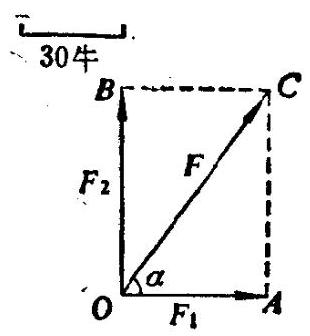
\includegraphics[max width=0.3\textwidth]{images/01912d55-147c-70aa-b0e0-1782a122f948_32_520124.jpg}
\end{center}

图 1-18

量得表示 \(F\) 的对角线长 25 毫米, 所以合力的大小,

\(F = {30}\) 牛 \(\times \frac{{25}\text{ 毫米 }}{{10}\text{ 毫米 }} = {75}\) 牛.

再用量角器可以量出合力 \(F\) 与 \({F}_{1}\) 的夹角 \(\alpha\) 为 \({53}^{ \circ }\) .

上题中分力 \({F}_{1}\) 与 \({F}_{2}\) 的夹角是 \({90}^{ \circ }\) ,所以 \({OACB}\) 是矩形, \(\bigtriangleup {OAC}\) 是直角三角形. 根据学过的几何知识可以知道 \({AC} =\) \({F}_{2},F\) 是直角三角形的弦. 因此在这种特殊情况下,合力 \(F\) 可以根据直角三角形的知识算出:

\[
F = \sqrt{{F}_{1}^{2} + {F}_{2}^{2}} = \sqrt{{\left( {45}\text{ 牛 }\right) }^{2} + {\left( {60}\text{ 牛 }\right) }^{2}}
\]

\[
= {754}\text{,}
\]

\[
\operatorname{tg}\alpha = \frac{{F}_{2}}{{F}_{1}} = \frac{604}{454} = {1.33},
\]

\[
\alpha = {53}^{ \circ }\text{. }
\]

\section*{练习四}

(1)四名同学一起玩拔河游戏. 其中两名分别用 280 牛和 350 牛的力向东拉, 另外两名分别用 300 牛和 340 牛的力向西拉. 求绳子所受的合力.

(2)图 1-19 表示两部拖拉机拉着一条船通过运河的情形. 如果两部拖拉机的拉力大小相等, 都是 2000 牛, 夹角是 \({50}^{ \circ }\) . 求这两个拉为的合力。

\begin{center}
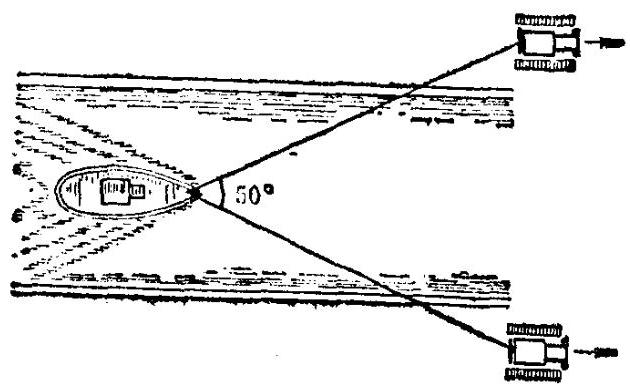
\includegraphics[max width=0.7\textwidth]{images/01912d55-147c-70aa-b0e0-1782a122f948_33_752107.jpg}
\end{center}

图 1-19

(3)两个共点力,大小都是 30 牛,夹角是 \({90}^{ \circ }\) . 求这两个力的合力.

(4)大小相等的两个共点力,求它们的夹角分别为 \({0}^{ \circ }\) 、 \({30}^{ \circ }\text{、}{60}^{ \circ }\text{、}{90}^{ \circ }\text{、}{120}^{ \circ }\text{、}{150}^{ \circ }\text{、}{180}^{ \circ }\) 时的合力. 比较求得的结果,能不能得出下面的结论: 合力总是大于分力; 夹角在 \({0}^{ \circ }\) 到 \({180}^{ \circ }\) 之间时, 夹角越大, 合力越小.

\section*{六、力的分解}

在许多实际问题中, 常常需要求一个已知力的分力. 例

\begin{center}
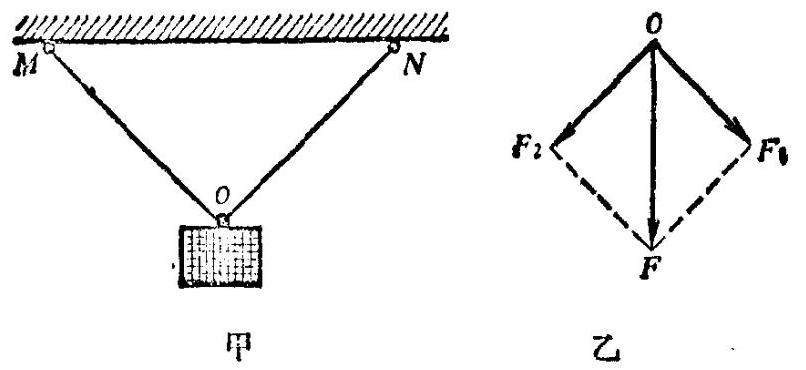
\includegraphics[max width=0.8\textwidth]{images/01912d55-147c-70aa-b0e0-1782a122f948_34_119901.jpg}
\end{center}

图 1-20

如, 照图 1-20 甲 那样, 把一个物体挂在成角度的两根绳 \({MO}\) 、 \({NO}\) 上,物体对悬挂点 \(O\) 的拉力 \(F\) 等于物体的重量 \(G\) ,方向是竖直向下的. 由于拉力 \(F\) 的作用, \({MO}\text{、}{NO}\) 也受到拉力作用(假如 \({MO}\text{、}{NO}\) 是橡皮筋,可以看出它们被拉长). \({MO}\text{、}{NO}\) 分别受到的拉力 \({F}_{1}\text{、}{F}_{2}\) 是拉力 \(F\) 的分力,要知道它们的大小和方向,就是一个求 \(F\) 的分力问题,或者说是一个力的分解问题.

力的分解是力的合成的逆运算, 同样遵守平行四边形法则. 把已知力作为平行四边形的对角线, 与已知力共点的平行四边形的两个邻边就是这个已知力的两个分力.

可是, 我们知道, 有相同对角线的平行四边形可以有无数个(图1-21), 也就是说, 同一个力可以分解为无数对大小、方向不同的分力. 要想得到确定的答案, 需要知道两个分力的方向或者一个分力的方向和大小. 那么, 一个已知的力究竟应该怎样分解呢? 这要根据实际问题来决定. 下面举两个具体实例.

\begin{center}
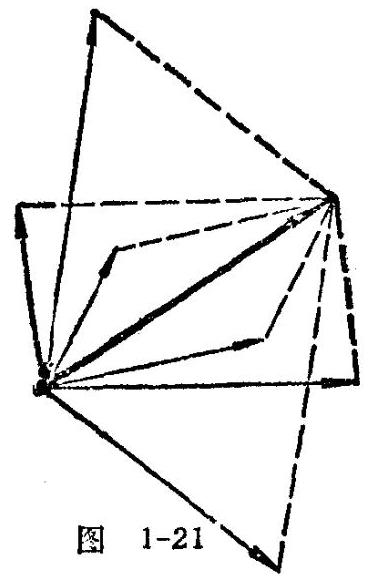
\includegraphics[max width=0.4\textwidth]{images/01912d55-147c-70aa-b0e0-1782a122f948_34_621679.jpg}
\end{center}

(1)一个物体放在斜面上, 物体受到竖直向下的重力作用, 但它并不竖直下落, 而是沿着斜面下滑, 同时压紧斜面. 这时,使物体平行于斜面下滑的力 \({F}_{1}\) ,和使物体垂直于斜面压紧斜面的力 \({F}_{2}\) ,都是重力 \(G\) 的分力. 要知道这两个分力,就需要把重力 \(G\) 沿这两个分力的方向分解.

在实际求 \({F}_{1}\) 和 \({F}_{2}\) 的时候,可以用作图法,即先选定一个标度,画出重力 \(G\) 的图示,再以表示 \(G\) 的线段 \({OP}\) 为对角线, 以平行于斜面的线段和垂直于斜面的线段为邻边, 作平行四边形(图 1-22),两个邻边 \({OR}\) 、 \({ON}\) 就分别表示使物体下滑的力 \({F}_{1}\) 和使物体压紧斜面的力 \({F}_{2}\) .

\begin{center}
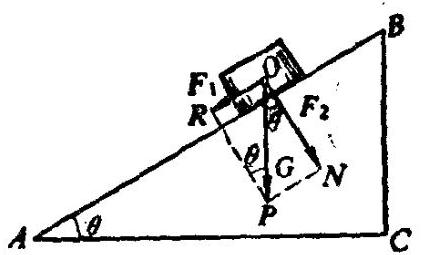
\includegraphics[max width=0.4\textwidth]{images/01912d55-147c-70aa-b0e0-1782a122f948_35_545044.jpg}
\end{center}

图 1-22

在已知重力 \(G\) 和斜面倾角 \(\theta\) 的情况下, \({F}_{1}\) 和 \({F}_{2}\) 的大小也可以计算出来. 根据几何知识知道,直角三角形 \({ABC}\) 与 \({OPN}\) 和 \({POR}\) 相似, \(\angle {PON} = \angle {OPR} = \theta\) ,所以

\[
{F}_{1} = G\sin \theta ,\;{F}_{2} = G\cos \theta .
\]

\({F}_{1}\text{、}{F}_{2}\) 的大小跟斜面的倾角有关. 斜面的倾角增大时, \({F}_{1}\) 增大, \({F}_{2}\) 减小. 车辆上桥时, 力 \({F}_{1}\) 阻碍车辆前进,车辆下桥时,力 \({F}_{1}\) 使车辆运动加快. 为了行车方便与安全, 高大的桥要造很长的引桥, 来减小桥面的倾角.

\begin{center}
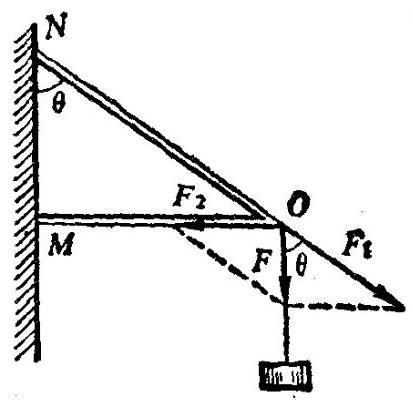
\includegraphics[max width=0.4\textwidth]{images/01912d55-147c-70aa-b0e0-1782a122f948_35_987792.jpg}
\end{center}

图 1-23

(2)把重量为 \(G\) 的物体挂在图 1-23 所示的支架上,物体通过绳子使支架上的 \(O\) 点受到一个向下的作用力 \(F\) ,大小等于物体的重量 \(G\) . 力 \(F\) 对支架的两根梁产生怎样的作用呢? 假如我们用橡皮筋代替斜梁,用手臂代替横梁,指尖顶在 \(O\) 处,从橡皮筋的伸长可以知道斜梁受到沿 \({NO}\) 方向的拉力,从手的感受可以知道横梁受到沿 \({OM}\) 方向的压力. 这个拉力 \({F}_{1}\) 和压力 \({F}_{2}\) 都是拉力 \(F\) 的分力,要知道这两个分力,就需要把拉力 \(F\) 沿 \({NO}\) 和 \({OM}\) 这两个方向分解.

实际求 \({F}_{1}\) 和 \({F}_{2}\) 的时候,可以用作图法. 如果支架是直角三角形,并且知道角 \(\theta\) 的值,也可以根据学过的数学知识算出 \({F}_{1}\) 和 \({F}_{2}\) 的大小:

\[
{F}_{1} = F/\cos \theta ,\;{F}_{2} = F\operatorname{tg}\theta .
\]

从上述两个例子可以看出, 在进行力的分解时, 一定要对具体事物进行具体分析. 先弄清楚所研究的力实际上产生了哪些效果, 然后再进行分解.

\section*{练 习 五}

(1)在图 1-22 中,重力 \(G\) 在垂直于斜面方向上的分力 \({F}_{2}\) ,等于物体对斜面的压力. 但是如果说 \({F}_{2}\) 就是物体对斜面的压力, 那就错了. 为什么?

(2)一位同学分析放在斜面上的物体的受力情况时说: “放在斜面上的物体, 受到四个力的作用: 地球对它的重力, 斜面对它的支持力, 斜面对它的摩擦力和下滑力. "你同意他的说法吗? 正确的说法是什么? 把这个物体受到的力示意地画出来。

(3)把竖直向下的 180 牛的力分解成两个分力, 使其中一个分力在水平方向上并等于 240 牛, 求另一个分力。

(4)绳的下端挂一个重 243 牛的物体, 由于有一条水平方向的拉链拉着物体,使绳静止在跟竖直方向成 \({45}^{ \circ }\) 角的位置. 求物体对水平拉链的拉力.

\begin{center}
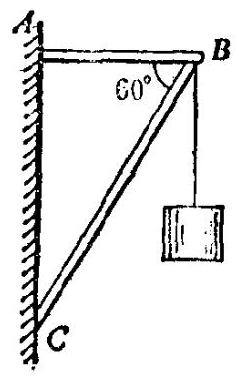
\includegraphics[max width=0.3\textwidth]{images/01912d55-147c-70aa-b0e0-1782a122f948_37_421617.jpg}
\end{center}

图 1-24

(5)在图1-24所示的直角三角形支架上, 挂着一个重量是 600 牛的物体,横梁 \({AB}\) 跟斜梁 \({BC}\) 的夹角是 \({60}^{ \circ }\) . 求作用于梁 \({AB}\) 和 \({BC}\) 上的力.

(6)一个骑自行车的人, 从倾角是 \({30}^{ \circ }\) 的斜坡向下滑行. 人和车的总重量是 700 牛. 求重力使车沿斜坡滑行的力和车对斜坡的压力.

\section*{七、共点力作用下物体的平衡}

我们经常可以看到, 一个物体在几个力的作用下, 保持静止或做匀速直线运动. 例如, 房屋、桥梁等受到重力和地面支持力的作用, 处于静止状态; 飞行中的飞机同时受到牵引力、 机翼的举力、重力、空气的阻力, 做匀速直线飞行. 物体处于静止或做匀速直线运动的状态叫做平衡状态. 要使物体保持平衡状态, 作用在物体上的力必须满足一定的条件, 这个条件叫做平衡条件.

研究物体的平衡很有实际意义. 工程技术上的很多物体, 例如桥梁、起重机、建筑物等, 都要保持平衡状态. 在设计桥梁、起重机、建筑物时, 必须分析它们各部分的受力情况, 然后根据平衡条件来进行计算, 以便确定几何尺寸或选择合适的材料.

现在先来研究在共点力作用下物体的平衡条件.

在初中已经学过, 物体受到两个共点力的时候, 只有这两个力大小相等、方向相反, 物体才保持平衡状态. 也就是说, 二力平衡的条件是: 两个力的大小相等, 方向相反, 并在同一直线上. 从力的合成可以知道, 这时作用力的合力等于零.

那么, 三个共点力作用下物体的平衡条件又是什么呢?

用三个弹簧秤水平地拉一个物体, 并使物体保持平衡状态(图 1-25 甲), 从三个弹簧秤上分别读出它们作用在物体上

\begin{center}
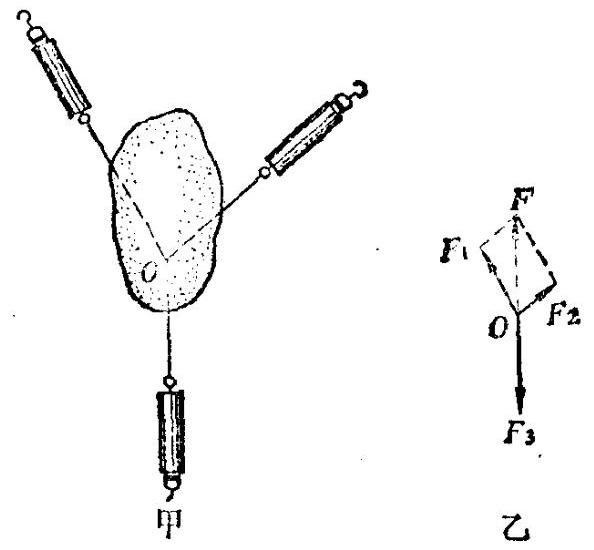
\includegraphics[max width=0.6\textwidth]{images/01912d55-147c-70aa-b0e0-1782a122f948_38_350265.jpg}
\end{center}

图 1-25

的拉力 \({F}_{1}\text{、}{F}_{2}\text{、}{F}_{3}\) 的大小,作出力的图示 (图 1-25 乙). 先求出其中任意两个力的合力,例如力 \({F}_{1}\) 和 \({F}_{2}\) 的合力 \(F\) . 可以看出,力 \(F\) 是和 \({F}_{3}\) 在同一直线上,大小相等、方向相反,它们的合力为零,也就是说, \({F}_{1}\text{、}{F}_{2}\text{、}{F}_{3}\) 的合力等于零. 可见,在三个共点力作用下物体的平衡条件是这三个力的合力等于零.

用实验可以同样证明, 在三个以上的共点力作用下物体的平衡条件也是合力等于零.

\begin{center}
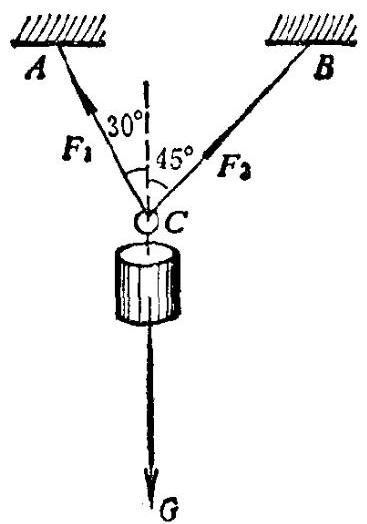
\includegraphics[max width=0.4\textwidth]{images/01912d55-147c-70aa-b0e0-1782a122f948_39_984528.jpg}
\end{center}

图 1-26

因此, 我们得到结论: 在共点力作用下物体的平衡条件是合力等于零.

[例题] 用绳 \({AC}\) 和 \({BC}\) 吊起一个物体(图 1-26), 物体的重量为 120 牛, 两根绳子和竖直线的夹角分别是 \({30}^{ \circ }\) 和 \({45}^{ \circ }\) , 求绳 \({AC}\) 和 \({BC}\) 对物体的拉力.

物体共受三个力的作用: 地球对物体的重力 \(G\) 和悬绳对物体的拉力 \({F}_{1}\text{、}{F}_{2}\) . 物体在这三个力作用下处于平衡状态. 根据前面讲的平衡条件可知, \({F}_{1}\text{、}{F}_{2}\) 的合力 \(F\) 必然与 \(G\) 在同一条直线上,而且大小相等、方向相反. 所以,可以先根据 \(G\) 作出 \(F\) 的图示,再将 \(F\) 分解求出 \({F}_{1}\text{、}{F}_{2}\) .

解: 选 10 毫米长的线段表示 30 牛的力.

作与 \(G\) 平衡的力 \(F = {120}\) 牛的图示. 在 \({AC}\text{、}{BC}\) 的方向上画出线段,以 \(F\) 为对角线作平行四边形, 如图 1-27 所示.

\begin{center}
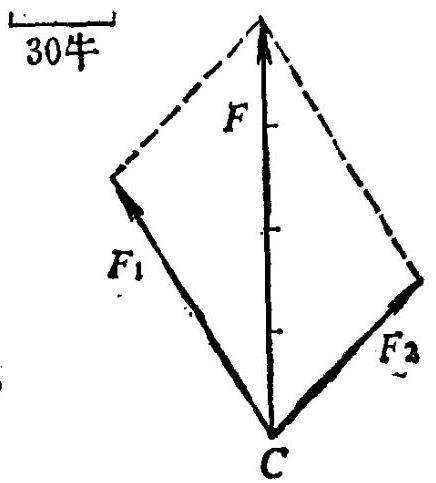
\includegraphics[max width=0.5\textwidth]{images/01912d55-147c-70aa-b0e0-1782a122f948_39_986758.jpg}
\end{center}

图 1-27

量得表示 \({AC}\) 拉力 \({F}_{1}\) 的边长 29 毫米,表示 \({BC}\) 拉力 \({F}_{2}\) 的边长 21 毫米. 所以

\[
{F}_{1} = {30}\text{ 牛 } \times \frac{{29}\text{ 毫米 }}{{10}\text{ 毫米 }} = {87}\text{ 牛,}
\]

\[
{F}_{2} = {30}\text{ 牛 } \times \frac{{21}\text{ 毫米 }}{{10}\text{ 毫米 }} = {63}\text{ 牛. }
\]

\section*{练习六}

(1)物体在三个力作用下处于平衡状态. 这三个力中有一个力的方向是水平向右, 大小是 10 牛. 如果去掉了这个力, 那么其余二力的合力是多大? 方向怎样?

(2)一名伞兵, 他的身体和全部装备(包括降落伞和武器等)的总重量是 800 牛. 当他匀速降落的时候, 他受到的空气阻力多大?方向怎样?

(3)用共点力平衡的知识来求练习五第 (4) 题中的水平拉链对物体的拉力.

(4)静止在斜面上的物体是在哪几个力的作用下平衡的? 如果物体的重量是 40 牛,斜面的倾角是 \({30}^{ \circ }\) . 求物体受到斜面的支持力和摩擦力.

\section*{八、有固定转动轴的物体的平衡}

房屋的门、窗, 工厂的砂轮、柴油机的飞轮、电动机的转子等等, 都能够绕着一个固定的轴转动. 这样的物体如果保持静止或者匀速转动(即在相等时间内转过相等的角度), 我们就说这个物体处于平衡状态.

能够转动的物体的平衡问题, 比较复杂. 我们只研究转动轴固定不动, 并且外力的作用线都在跟转动轴垂直的平面内的情况.

力矩 推门时, 力作用在离门轴较远的地方, 用较小的力就可以把门推开; 如果在离门轴不远的地方推门, 就要用较大的力才能把门推开. 拧螺帽时, 扳柄长一些, 就比较容易把螺帽拧紧. 可见, 力使物体转动的效果, 不仅跟力的大小有关, 还跟力和转动轴的距离有关. 力越大, 力跟转动轴的距离越大, 力使物体转动的作用就越大.

从转动轴到力的作用线的垂直距离, 叫做力臂. 图1-28 表示有两个力 \({F}_{1}\) 和 \({F}_{2}\) 作用在杠杆上,杆的转动轴 \(O\) 垂直于纸面, \({L}_{1}\) 是力 \({F}_{1}\) 的力臂, \({L}_{2}\) 是力 \({F}_{2}\) 的力臂.

\begin{center}
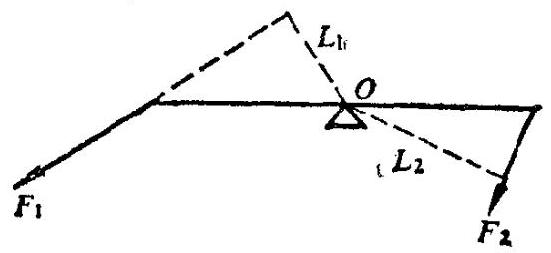
\includegraphics[max width=0.6\textwidth]{images/01912d55-147c-70aa-b0e0-1782a122f948_41_796144.jpg}
\end{center}

图 1-28

力和力臂的乘积叫做力对转动轴的力矩. 用 \(F\) 表示力的大小, \(L\) 表示力臂, \(M\) 表示力矩,那么,

\[
M = {FL}\text{.}
\]

力矩可以使物体向不同的方向转动. 例如开门和关门时, 门的转动方向相反. 拧紧螺帽和拧松螺帽时, 螺帽的转动方向也相反.

力矩的单位由力和力臂的单位决定. 如果力的单位用牛顿, 力臂的单位用米, 力矩的单位就是牛顿一米. 简称牛. 米. 国际符号是 \(\mathrm{N} \cdot \mathrm{m}\) .

有固定转动轴的物体的平衡 有固定转动轴的物体的平衡条件是什么呢? 我们用图 1-29 所示的力矩盘来研究这个问题.

首先使圆盘在力 \({F}_{1}\text{、}{F}_{2}\text{、}{F}_{3}\) 和 \({F}_{4}\) 的作用下处于平衡状

\begin{center}
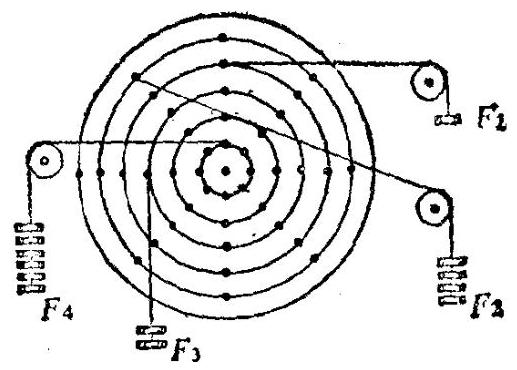
\includegraphics[max width=0.5\textwidth]{images/01912d55-147c-70aa-b0e0-1782a122f948_42_728486.jpg}
\end{center}

图 1-29

态. 量出这四个力的力臂 \({L}_{1}\text{、}{L}_{2}\text{、}{L}_{3}\) 和 \({L}_{4}\) ,分别算出它们的力矩 \({M}_{1} = {F}_{1}{L}_{1},{M}_{2} = {F}_{2}{L}_{2},{M}_{3} = {F}_{3}{L}_{3},{M}_{4} = {F}_{4}{L}_{4}\) ,发现使圆盘向顺时针方向转动的力矩之和等于使圆盘向反时针方向转动的力矩之和, 即

\[
{M}_{1} + {M}_{2} = {M}_{3} + {M}_{4}
\]

改变力和力臂再做这个实验, 可以得到同样的结果. 可见, 有固定转动轴的物体的平衡条件, 是使物体向顺时针方向转动的力矩之和, 等于使物体向反时针方向转动的力矩之和.

[例题] 图 1-30 甲中的 \({OB}\) 是一根水平横梁,长 1.0 米, 一端安装在轴 \(O\) 上,另一端用绳子 \({AB}\) 拉着. 如果在横梁上距离 \(O\) 点 80 厘米处挂一个 50 牛的重物,绳子对横梁的拉力是多大?

\begin{center}
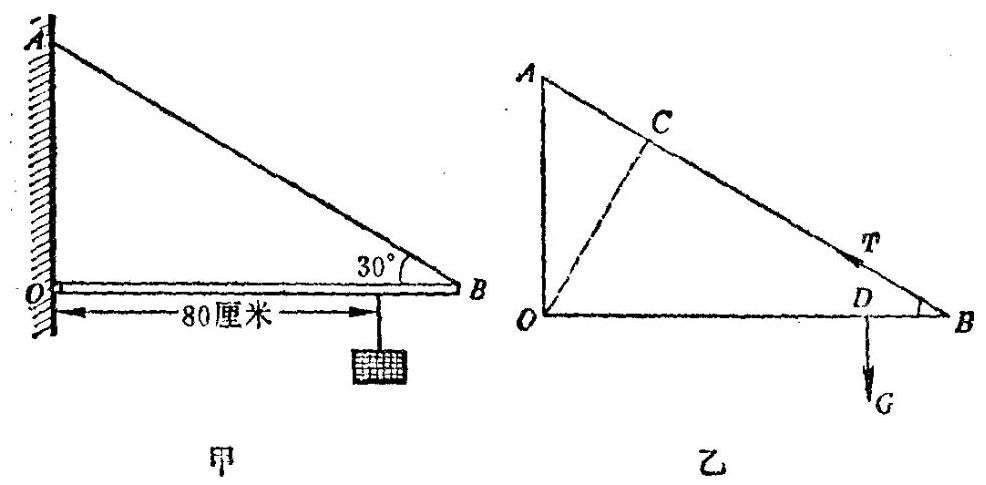
\includegraphics[max width=1.0\textwidth]{images/01912d55-147c-70aa-b0e0-1782a122f948_42_933056.jpg}
\end{center}

图 1-30

横梁是一个有固定转动轴的物体, 图 1-30 乙表示它的受力情况,其中 \(T\) 是绳子对横梁的拉力,它的力矩 \({M}_{1} = T \cdot {OC}\) 要使横梁反时针方向转动, \(G\) 是重物通过悬绳对横梁的拉力,它的力矩 \({M}_{2} = G \cdot {OD}\) 要使横梁顺时针方向转动. 横梁处于平衡状态,根据平衡条件 \({M}_{1} = {M}_{2},T \cdot {OC} = G \cdot {OD}\) ,其中 \(G\) 和 \({OD}\) 是已知的,根据横梁的长度和夹角的值求出 \({OC}\) ,就可以算出拉力 \(T\) .

解: \(T\) 对轴 \(O\) 的力臂 \({OC} = {OB} \times \sin {30}^{ \circ } = {0.50}\) 米.

\(T\) 对轴 \(O\) 的力矩 \({M}_{1} = T \cdot {OC}\) . (反时针方向)

\(G\) 对轴 \(O\) 的力矩 \({M}_{2} = G \cdot {OD}\) . (顺时针方向)

由 \({M}_{1} = {M}_{2}\) 得 \(T \cdot {OC} = G \cdot {OD}\) ,

所以, 绳子对横梁的拉力

\[
T = \frac{G \cdot {OD}}{OC} = \frac{{50}\text{ 牛 } \times {0.80}\text{ 米 }}{{0.50}\text{ 米 }} = {80}\text{ 牛. }
\]

\section*{练习七}

(1)当我们开关门窗时, 如果作用力通过转轴, 那么, 无论多大的力也不能把门窗打开或关上, 为什么?

(2)一根杠杆,转动轴是 \(O\) . 我们在杠杆上的一点 \(A\) 加一个能使杠杆转动的力 \(F.F\) 对轴 \(O\) 的力臂,能不能小于、等于或大于轴到力的作用点的距离 \({OA}\) ? 为什么?

(3)自行车车轮的轮缘和闸皮间的摩擦力是 20 牛, 如果车轮的半径是 0.35 米. 求摩擦力的力矩.

\begin{center}
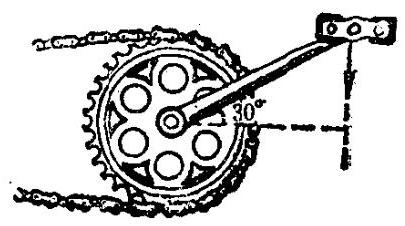
\includegraphics[max width=0.4\textwidth]{images/01912d55-147c-70aa-b0e0-1782a122f948_44_653949.jpg}
\end{center}

图 1-31

(4)如图 1-31 所示, 加在自行车脚踏板上的向下的力是 15 牛, 脚踏板的受力点到转动轴的距离是 17.5 厘米. 求这个力的力矩.

(5)前面的例题中, 我们忽略了横梁和绳子本身的重量. 如果绳子重量可以忽略, 而横梁是根均匀的铁棒, 重量是 60 牛, 不能忽略. 那么这时绳对横梁的拉力是多大?

(6)力矩盘受到三个力的作用, 其中使盘向顺时针方向转动的两个力是 5 牛和 3 牛, 使盘向反时针方向转动的力是 2 牛. 这三个力的力臂依次是 5 厘米、10厘米、30厘米. 在这三个力作用下, 力矩盘是否平衡? 为了使力矩盘平衡, 要给力矩盘再加一个 1 牛的作用力, 这个作用力的力臂应该多大? 它的作用是要使力矩盘向哪个方向转动?

\section*{小 实 验}

学习了物体平衡的知识, 你可以自己制作一把杆秤, 来了解用杆秤称物体质量的道理.

找一根 30 10 厘米长的细木棍作秤杆,一个质量为 \(\frac{1}{4}\) 千克左右的物体作秤锤. 先确定秤钩和提纽的位置. 然后在秤钩不挂物体的情况下, 照图 1-32 那样把秤锤挂在秤杆上, 提起提纽, 使秤杆平衡, 秤锤的位置就是秤的零刻度(也叫定盘

\begin{center}
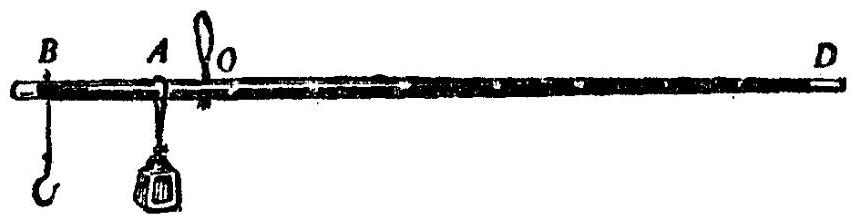
\includegraphics[max width=0.9\textwidth]{images/01912d55-147c-70aa-b0e0-1782a122f948_45_871328.jpg}
\end{center}

图 1-32

星). 再把质量为 100 克的物体挂在秤钩上, 调整秤锤的位置, 使秤杆平衡, 这时秤锤的位置就是秤的 100 克刻度. 再在秤钩上挂质量为 200 克、300 克的物体, 使秤杆平衡, 找出 200 克、300 克刻度的位置. 你将发现 100 克、200 克、300 克刻度与零刻度的距离正好是 \(1 : 2 : 3\) . 即秤锤离零刻度的距离跟被 称物体的质量成正比. (为什么? 有兴趣的同学可以自己证明.) 根据这个规律, 你可以在秤杆上找出 400 克、500 克等刻度的位置. 把相邻两个刻度间的距离等分成 10 份, 每份间的距离就代表 10 克. 这样你的杆秤就做成了.

请你想一想, 在制作杆秤的过程中, 秤杆每一次处于平衡状态时, 顺时针转动的力矩, 反时针转动的力矩各是什么?

\section*{九、平衡的种类和稳度*}

平衡的种类 儿童玩的不倒翁 (图 1-33 甲), 钢丝上的杂技演员 (图 1-34), 都是在重力和支持物作用下处于平衡状态. 但是, 不倒翁扳倒后总会自动竖起, 逗得孩子们开心地笑, 钢丝上的演员稍有差错就会摔下来, 让观众捏一把汗. 可见, 都属于平衡状态, 也还存在差别. 差别在哪里呢? 我们用实验来研究这个问题.

\begin{center}
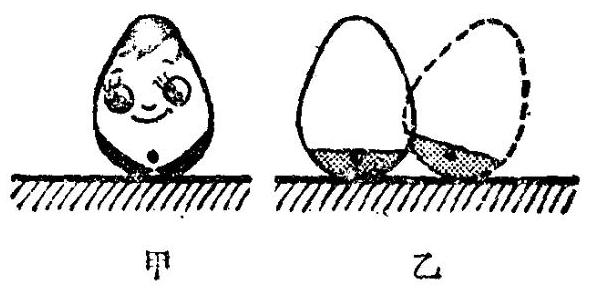
\includegraphics[max width=0.6\textwidth]{images/01912d55-147c-70aa-b0e0-1782a122f948_46_603417.jpg}
\end{center}

图 1-33 不倒翁

\begin{center}
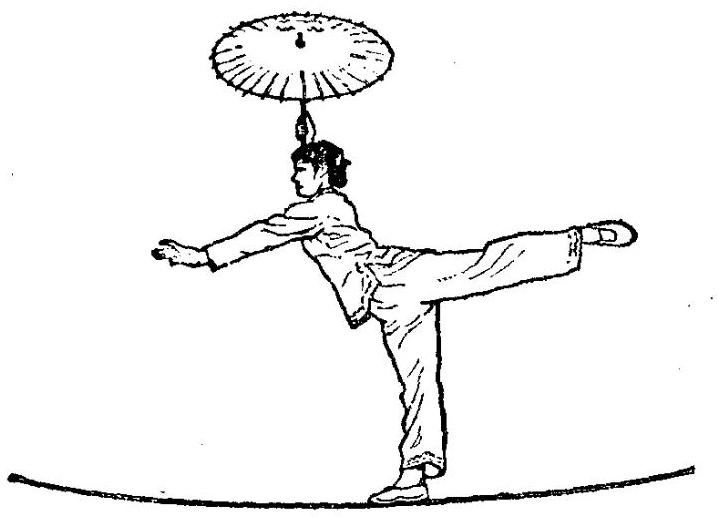
\includegraphics[max width=0.8\textwidth]{images/01912d55-147c-70aa-b0e0-1782a122f948_46_750520.jpg}
\end{center}

图 1-34

照图 1-35 甲那样,把木条一端的孔套在水平轴 \(O\) 上,把木条从平衡位置稍微移开一点,重心 \(C\) 的位置升高,重力的力矩就使它回到原来的平衡位置, 这种平衡叫稳定平衡.

\begin{center}
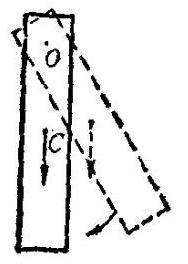
\includegraphics[max width=0.2\textwidth]{images/01912d55-147c-70aa-b0e0-1782a122f948_46_222690.jpg}
\end{center}

\begin{center}
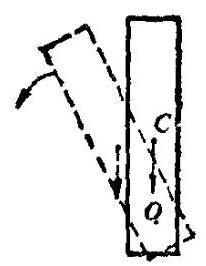
\includegraphics[max width=0.2\textwidth]{images/01912d55-147c-70aa-b0e0-1782a122f948_46_155633.jpg}
\end{center}

\begin{center}
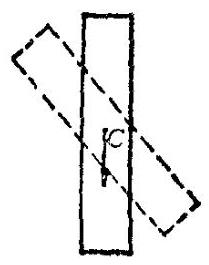
\includegraphics[max width=0.2\textwidth]{images/01912d55-147c-70aa-b0e0-1782a122f948_46_302446.jpg}
\end{center}

即 乙 丙

图 1-35 稳定平衡 (甲), 不稳平衡 (乙), 随遇平衡 (丙)

照图 1-35 乙那样, 使木条的重心恰好在水平轴的正上方, 木条处于平衡. 把木条从平衡位置稍微移开一点, 重心的位置降低, 重力的力矩就使它继续远离平衡位置, 这种平衡叫不稳平衡.

照图 1-35 丙那样,把木条重心 \(C\) 处的孔套在轴 \(O\) 上,无论把木条拔到任何位置, 它都能保持平衡, 这是因为它的重心高度没有改变. 这种平衡叫随遇平衡.

可见, 物体在重力和支持物作用下的平衡可以分为稳定平衡、不稳平衡和随遇平衡. 物体稍微偏离平衡位置, 如果重心升高, 就是稳定平衡, 如果重心降低, 就是不稳平衡, 如果重心的高度不变, 就是随遇平衡.

不倒翁的底部是泥块, 上部是空的, 竖立的时候重心位置最低 (图 1-33 乙), 处于稳定平衡, 无论怎样扳动, 它的重心都要升高, 所以它总会自动竖起.

钢丝上的杂技演员, 处于不稳平衡. 杂技演员就是凭借她掌握不稳平衡的高超技巧, 以惊险而优美的动作, 牵动观众们的心.

机器上高速旋转的部件, 如电动机的转子、汽轮机的叶轮, 都必须调整为随遇平衡, 不然运转起来会产生有害振动, 使机器损坏.

稳度 平放的砖和竖放的砖, 都处于稳定平衡状态(图1- 36), 稍微离开平衡位置, 重心都升高. 但是, 它们的稳定程度不同. 竖放的砖容易翻倒, 而平放的砖不容易翻倒. 我们把稳定程度叫做稳度.

从图 1-36 可以看出, 平放的砖, 重心低、底面积大, 只有

\begin{center}
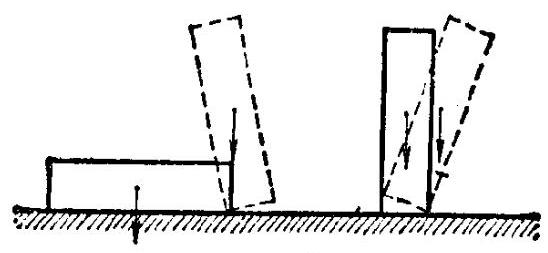
\includegraphics[max width=0.6\textwidth]{images/01912d55-147c-70aa-b0e0-1782a122f948_48_300670.jpg}
\end{center}

图 1-36

使它偏转很大的角度, 它的重力作用线才会超出支棱使它向外翻倒. 竖放的砖, 重心高、底面积小, 只要偏转不大的角度, 重力作用线就会超出支棱使砖向外翻倒. 可见, 物体的重心越低、底面积越大, 稳度越大.

增大物体的稳度有重要的实际意义. 为了增大物体的稳度, 既可以增大底面的面积, 也可以降低重心的高度, 还可以同时增大底面面积和降低重心的高度. 实验用的天平要安置在一个底面面积较大而又较重的底座上, 实验用的铁架都有一个面积较大的铸铁座, 照相机要安放在支面相当大的三脚架上, 高压线的铁塔都有一个很大的支面, 工厂烟囱底面的直径比顶部的直径要大一些, 越野汽车和山区用的拖拉机轮间宽度较宽, 都是为了增大物体的稳度.

\section*{阅读材料: 侯风地动仪}

我国汉代科学家张衡 \(\left( {{78} \sim {139}}\right)\) 在公元 132 年发明的候风地动仪 (彩图 1), 是利用柱摆稳度小的特性来测定地震震源方向的仪器.

候风地动仪是用青铜铸成的, 直径八尺, 外壁上均匀分布着八条龙, 龙嘴里含着小铜球, 龙头各向一方. 在龙头下面的地上蹲着八个昂首张口的铜蛤蟆, 龙嘴里含着的小铜球落下来的时候, 正好落在蛤蟆嘴里.

\begin{center}
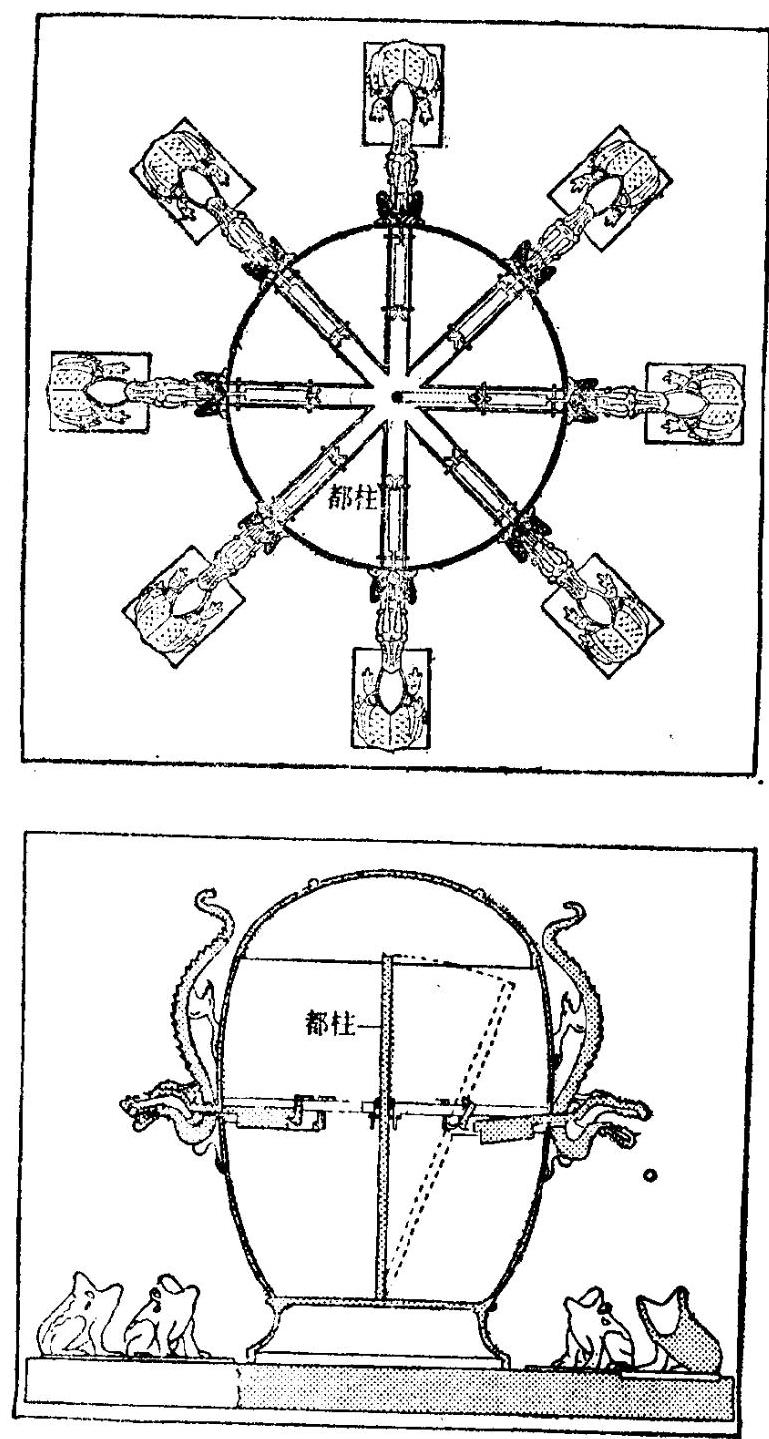
\includegraphics[max width=0.8\textwidth]{images/01912d55-147c-70aa-b0e0-1782a122f948_49_654467.jpg}
\end{center}

图 1-37 候风地动仪的构造

(上) 下视图 (下) 纵截面图

图 1-37 是候风地动仪的内部构造. 仪器的中央竖立着一根铜体的柱摆, 原名都柱. 由于它的重心高, 支面小, 稳度小, 所以受到振动容易失去平衡. 柱摆的周围有八组跟龙嘴上唇相连的杠杆.

候风地动仪的工作原理是, 从某个方向发出的地震的振动传到地动仪的时候, 柱摆由于惯性就倒向震源的方向, 结果这个方向上的杠杆就被推动, 跟这组杠杆相连的龙嘴就张开, 小铜球就落到它下面的蛤蟆嘴里. 所以看哪个龙嘴里的小铜球下落, 就知道哪个方向发生地震. 在候风地动仪制成后不久, 的确用它正确地测出过震源的方向. 根据《后汉书》的记载: “尝一龙机发, 而地不觉动, 京师学者, 咸怪其无征. 后数日, 驿至, 果地震陇西, 于是皆服其妙. ”可见, 在当时的首都洛阳已经能记录到甘肃的地震了. 这个仪器的发明, 比欧洲人制造的测量地震的类似仪器要早一千七百多年.

\section*{练 习 八}

(1) 图 1-38 中的两个质量分布均匀的球是处于平衡状态吗? 是什么平衡?

\begin{center}
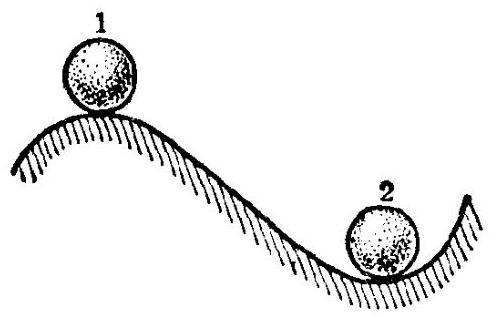
\includegraphics[max width=0.5\textwidth]{images/01912d55-147c-70aa-b0e0-1782a122f948_50_768281.jpg}
\end{center}

图 1-38

\begin{center}
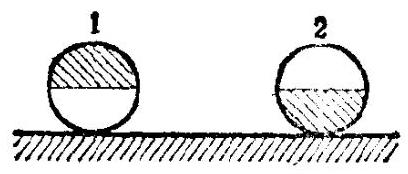
\includegraphics[max width=0.4\textwidth]{images/01912d55-147c-70aa-b0e0-1782a122f948_50_275942.jpg}
\end{center}

图 1-39

(2)图 1-39 所示的两个质量分布不均匀的球, 是处于平衡状态吗? 是什么平衡 (球上画有斜线的那一半是用密度较大的物质做的)?

(3)背上背着东西的人, 为什么要向前倾?

(4)用载重汽车装运木箱, 一些木箱装满了铁钉, 另一些木箱装满铝锅. 怎样装这些木箱, 汽车的稳度比较大?

(5)找一块形状不规则的硬纸片, 先找到它的重心, 然后用这块硬纸片, 设计一个稳定平衡的悬挂法、一个不稳平衡的悬挂法和一个随遇平衡的悬挂法. 实际作作看.

\section*{小 实 验}

照图1-40那样, 在水平桌面上放一块木板, 再把一个长方体木块竖放在木板上. 在木块正面的中心点固定一个螺钉, 螺钉上拴一个小重锤. 然后将木板的一端慢慢抬起, 观察重锤到什么位置时, 木块才会倾倒.

\begin{center}
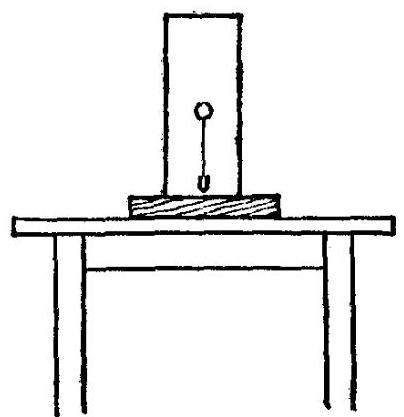
\includegraphics[max width=0.4\textwidth]{images/01912d55-147c-70aa-b0e0-1782a122f948_51_707316.jpg}
\end{center}

图 1-40

\section*{复习 题}

(1)什么是力? 从力的性质看, 力学中经常遇到的有哪几种力?

(2)什么是弹力?什么是胡克定律?举几个弹力的实例.

(3)写出计算滑动摩擦力的公式. 滑动摩擦力的方向是怎样的?

(4)什么叫力的合成? 力的合成按照什么法则来进行? 这个法则的内容是什么?

(5)什么叫矢量? 什么叫标量? 矢量相加按照什么法则进行?

(6)什么叫力的分解?力的分解按照什么法则进行? 在具体分解一个力的时候, 如果知道两个分力的方向, 或者知道一个分力的方向和大小, 这个力的分解有没有确定的答案?

(7)共点力作用下物体的平衡条件是什么?

(8)什么叫力矩? 力矩的单位是什么?

(9)有固定转动轴的物体的平衡条件是什么?

(10)什么是稳定平衡? 什么是不稳平衡? 什么是随遇平衡? 举例说明.

(11)什么叫稳度? 怎样才能增大物体的稳度? 举几个实例来说明.

\section*{习 题}

(1)雨滴下落的时候, 空气阻力不能忽略不计. 质量是 \({1.0} \times {10}^{-4}\) 千克的雨滴,在无风的时候匀速竖直下落,作出雨滴受力的图示.

(2)一个重量是 20 牛的物体静止在倾角为 \({30}^{ \circ }\) 的斜面上, 求斜面对它的静摩擦力。

(3)在同一平面上的三个共点力, 它们之间的夹角都是 \({120}^{ \circ }\) ,大小分别是 20 牛、30 牛、40 牛. 求这三个力的合力.

(4)马拉着重 8000 牛的车, 沿着一段坡路匀速前进. 在这段坡路上, 每前进 15.0 米, 高度升高 1.0 米。如果不考虑车轮跟地面间的摩擦, 马的拉力是多大?

(5)两手握着橡皮筋的两端, 在橡皮筋的中间挂一个重物. 当两手间的距离增加的时候, 橡皮筋的长度是不是改变? 实际做一做, 并解释看到的现象.

(6)一块重量是 75 牛的木块, 在 5.0 牛的拉力作用下, 在冰面上匀速前进. 如果拉力的方向斜向上方, 跟水平方向间的夹角是 \({60}^{ \circ }\) ,木块在水平方向受到的拉力有多大? 木块对冰面的压力有多大? 木块跟冰面间的滑动摩擦系数是多大?

(7)如果图 1-32 中的杆秤提扭和挂钩的距离 \({OB} = {6.0}\) 厘米,秤锤的质量是 1.2 斤. 定盘星到提扭的距离 \({AO} = {1.6}\) 厘米. 秤杆的质量是 0.48 斤, 求秤杆重心的位置. 在称某一物体时, 秤锤移到 \(D\) 点后杆秤平衡, \({AD} = {24}\) 厘米,求所称物体的质量.

\section*{第二章 直 线 运 动}

在初中我们学过, 一个物体相对于别的物体的位置改变叫做机械运动, 简称运动. 机械运动是最普遍的自然现象. 宇宙中的一切物体, 小到原子内部的质子、中子和电子, 大到遥远的恒星和星系, 都在不停地运动着. 有些物体, 例如耸立的山峰、马路两侧的房屋、路面上的铁轨, 看起来是不动的, 其实, 这些物体是随着地球一起运动的.

由于一切物体都在运动, 我们在研究物体的运动时, 就必须假定某个物体是不动的, 参照这个物体来确定其他物体的运动. 例如, 我们说火车是运动的、桥梁是静止的, 是以地面作参照来说的. 我们说地球是运动的, 是以太阳作参照来说的. 为了研究物体的运动而假定为不动的那个物体, 叫做参照物.

同一个运动, 由于选择的参照物不同, 观察的结果常常是不同的. 例如, 火车车厢里的乘客, 选车厢作参照物, 认为自已是静止的. 站在铁路旁边的人, 选地球作参照物, 认为乘客是随着车厢一起运动的. 在研究地面上物体的运动时, 为了研究问题的方便, 常取地球作参照物. 在这一章里, 我们只研究以地球为参照物并且运动路线是直线的运动.

\section*{一、质点 位移和路程}

质点 研究物体的运动, 第一步是要确定物体的位置. 物体都具有大小和形状, 在运动中物体中各点的位置变化一般说来是各不相同的, 所以要详细描述物体的位置及其变化, 并不是一件简单的事情. 为了便于着手研究, 物理学采用的方法是先做一些简化, 不考虑物体的大小和形状, 而把物体看作一个有质量的点, 或者说用一个有质量的点来代替整个物体. 用来代替物体的有质量的点叫做质点.

物理学对实际问题的简化, 也叫科学抽象, 不是随心所欲的, 必须从实际出发, 撇开不考虑的只能是与当前考察无关的因素, 和对当前考察影响很小的次要因素.

在什么情况下物体的大小、形状属于无关因素或次要因素呢? 这要看具体情况而定. 举例来说, 一个物体, 如果它的各个部分的运动情况都相同, 那么, 在研究这个物体的运动规律时, 它的任何一点的运动, 都可以代表整个物体的运动. 在这种情况下, 物体的大小、形状就无关紧要了, 可以把整个物体当作质点. 在平直公路上行驶的汽车, 车身上各部分的运动情况相同, 当我们把汽车作为一个整体来研究它的运动的时候, 就可以把汽车当作质点. 当然, 假如我们需要研究汽车的轮胎的运动, 由于轮胎的各部分的运动情况不相同, 那就不能把它看作质点了.

当我们研究地球的公转时,由于地球的直径 (约 \({1.3} \times {10}^{4}\) 千米) 比地球和太阳之间的距离 (约 \({1.5} \times {10}^{8}\) 千米) 要小得多, 地球上各点相对于太阳的运动, 差别极小, 可以认为相同, 即地球的大小和形状可以忽略不计, 而把地球当作质点. 可是在研究地球的自转时, 地球的大小和形状不能忽略, 当然不能把地球当作质点了.

在这一章和以后各章中, 我们所研究的物体, 除非涉及到转动, 一般都可以把它们当作质点.

\begin{center}
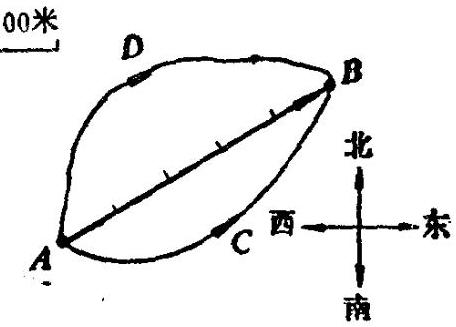
\includegraphics[max width=0.5\textwidth]{images/01912d55-147c-70aa-b0e0-1782a122f948_56_530856.jpg}
\end{center}

图 2-1 位移和路程

位移和路程 假如你的家在图 2-1 的 \(A\) 点,学校在 \(B\) 点, 即在你家东偏北 \({30}^{ \circ }\) 方向 500 米处,从你家到学校,可能有长短不同的几条路. 但是如果只考虑你位置的改变, 即你的位移,那么无论走哪条路,你的位移都是向东偏北 \({30}^{ \circ }\) 方向移动了 500 米. 表示这个位移最简单的方法, 是用一根带箭头的线段, 箭头表示位移的方向, 线段的长度表示位移的大小.

位移不但有大小, 而且有方向, 是一个矢量.

位移跟我们在初中学过的路程是不同的物理量. 在图 2-1 中,如果走 \({ACB}\) 这条路,路程就是曲线 \({ACB}\) 的长度,如果走 \({ADB}\) 这条路,路程就是曲线 \({ADB}\) 的长度. 不过,如果你走的是 \({AB}\) 这条直路,用物理的话来说,就是沿直线向某一方向运动, 那么通过的路程就等于位移的大小了.

\section*{练 习 -}

(1) 一位同学沿着东西方向的马路向西走了 400 米, 买了信封、信纸, 又向东走了 100 米来到邮局. 他总共走了多少路程? 邮局离他出发点多远? 邮局在出发点的东边还是西边?

(2)一辆汽车向东行驶了 40 千米, 又向南行驶了 30 千米, 求汽车位移的大小和方向.

\section*{二、匀速直线运动 速度}

我们研究物体的运动, 就是要掌握它的运动规律, 以便预测经过一段时间后物体的位移怎样, 速度怎样, 以及它在这段时间内的运动轨迹. 也许, 研究物体的运动应该从最常见的运动着手吧! 一片树叶从树上下落是常见的运动, 但是它忽左忽右, 时快时慢, 运动情况十分复杂, 不便于研究. 在物理学中研究问题, 一般都不是从复杂的现象着手, 而是从便于研究的简单现象着手, 我们研究物体的运动, 就从简单的匀速直线运动开始. 将来你能体会到从简单现象着手是一种十分有益的研究方法.

匀速直线运动 汽车在平直的公路上行驶, 如果每分钟的位移是 600 米, 每秒钟的位移是 10 米, 也就是在相等时间内的位移相等, 我们就说汽车的运动是匀速直线运动.

物体在一条直线上运动. 如果在相等的时间里位移相等, 这种运动就叫做匀速直线运动. 匀速直线运动又简称为匀速运动.

速度 一辆做匀速运动的卡车, 如果每秒内的位移是 10 米,那么它在 \(1\text{、}2\text{、}3\cdots \cdots\) 秒内的位移就是 \({10}\text{、}{20}\text{、}{30}\cdots \cdots\) 米, 位移和时间的比值 \(\frac{{10}\text{ 米 }}{1\text{ 秒 }} = \frac{{20}\text{ 米 }}{2\text{ 秒 }} = \frac{{30}\text{ 米 }}{3\text{ 秒 }}\cdots \cdots\) 是个恒量. 一辆做

匀速运动的小汽车, 如果每秒内的位移是 20 米, 那么它在 1 、 \(2\text{、}3\cdots \cdots\) 秒内的位移就是 \({20}\text{、}{40}\text{、}{60}\cdots \cdots\) 米,位移和时间的比值 \(\frac{{20}\text{ 米 }}{1\text{ 秒 }} = \frac{{40}\text{ 米 }}{2\text{ 秒 }} = \frac{{60}\text{ 米 }}{3\text{ 秒 }}\cdots \cdots\) 也是个恒量. 位移和时间的比值有什么意义呢? 从举的卡车和小汽车运动的例子可以看出, 这个比值越大, 表示运动越快, 比值越小, 表示运动越慢 (图 \(2 - 2)\) .

\begin{center}
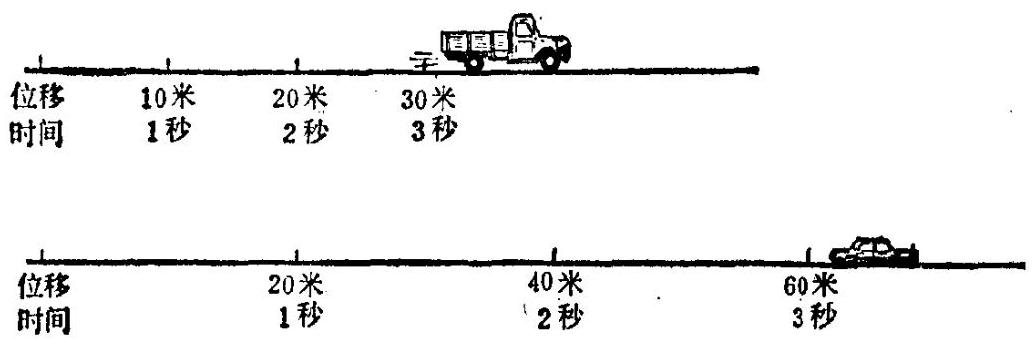
\includegraphics[max width=1.0\textwidth]{images/01912d55-147c-70aa-b0e0-1782a122f948_58_163927.jpg}
\end{center}

图 2-2

在匀速直线运动中, 位移跟时间的比值, 叫做匀速直线运动的速度.

做匀速运动的物体,如果在时间 \(t\) 内的位移是 \(s\) ,它的速度 \(v\) 就是

\[
v = \frac{s}{t}
\]

由上式可以看出, 速度在数值上等于单位时间内位移的大小.

速度的单位在国际单位制中是米/秒, 读作米每秒. 常用的单位还有千米/小时, 厘米/秒等.

速度不但有大小, 而且有方向, 是个矢量. 速度的方向与位移的方向相同. 在匀速直线运动中, 速度的方向和大小都不变. 速度的大小叫速率.

知道匀速运动物体的速度, 我们就能准确地预测物体在给定时间内的位移, 或者预测物体通过某段距离需要用多少时间.

例如, 一辆汽车以 20 米/秒的速度向东匀速行驶, 求它 1 分钟的位移. 我们可以把 \(v = \frac{s}{t}\) 变形,得到

\[
s = {vt}\text{.}
\]

这个公式叫匀速运动的位移公式. 把 \(v = {20}\) 米/秒、 \(t = 1\) 分 \(= {60}\) 秒代入位移公式,就求出汽车 1 分钟的位移是 1.2 千米, 方向向东.

如果求这辆汽车行驶 6.0 千米需要多长时间. 可以将 \(v\) \(= \frac{s}{t}\) 变形为

\[
t = \frac{s}{v}
\]

把 \(v = {20}\) 米 \(/\) 秒和 \(s = {6.0}\) 千米 \(= {6.0} \times {10}^{3}\) 米代入上式,就求出需要用的时间 \(t = {3.0} \times {10}^{2}\) 秒 \(= {5.0}\) 分.

\section*{练习二}

(1) 千米/小时是交通运输中常用的速度单位. 试求 1 米/秒合多少千米/小时.

(2)一位乘客测出火车每 5.0 分钟的位移是 5.0 千米, 你帮助他计算一下火车的速度是多少米/秒, 多少千米/小时.

(3)请你用一只带秒针的普通的表, 测出自己脉搏跳动一次的平均时间. 如果汽车的速度是 80 千米/小时, 飞机的速度是 900 千米/小时, 在你的脉搏跳动一次的平均时间里, 汽车和飞机各前进了多远?

(4)在真空中光的速率是 \({3.0} \times {10}^{8}\) 米/秒,太阳距地球 \({1.5} \times {10}^{11}\) 米远. 求光从太阳传到地球需要用多少秒钟.

\section*{三、匀速直线运动的图象}

物体运动的规律不但可以用公式来表示, 还可以用图象来表示. 表示位移和时间的关系的图象, 叫位移-时间图象, 可以简称为位移图象. 表示速度和时间关系的图象, 叫速度- 时间图象, 可以简称为速度图象.

图象通常是根据实验测定的数据作出的.

例如, 我们要研究一辆汽车在一段公路上运动的情况, 可以在公路旁每隔 100 米站一名拿着秒表的观测者, 记下汽车到达每个观测者的时间 (图 2-3). 把测量的结果记在下面的表里.

\begin{center}
\includegraphics[max width=0.9\textwidth]{images/01912d55-147c-70aa-b0e0-1782a122f948_60_988298.jpg}
\end{center}

图 2-3

在平面直角坐标系中,以纵轴表示位移 \(s\) 的值,横轴表示时间,标出表示 \(\left( {{4.9},{100}}\right) \text{、}\left( {{10.0},{200}}\right) \text{、}\left( {{15.1},{300}}\right) \text{、}({19.9}\) , 400)的点. 每个点代表一对数据. 可以看出各个点几乎都在一条通过原点的直线上, 有的点略微偏离这条直线 (图 2-4), 我们相信这是由于测量误差引起的. 画出这条直线, 就得到

\begin{center}
\includegraphics[max width=1.0\textwidth]{images/01912d55-147c-70aa-b0e0-1782a122f948_61_851196.jpg}
\end{center}

图 2-4 匀速直线运动的位移图象

汽车的位移图象.

从位移图象可以了解物体运动的许多情况. 在图 2-4中, 图象是过原点的直线. 从数学课知道, 过原点的直线表示正比例函数,即时间 \(t\) 增大几倍,位移 \(s\) 也增大几倍,或者说 \(\frac{s}{t} =\) 恒量. 而 \(\frac{s}{t} = v,v\) 是恒量,表示汽车是做匀速运动. 根据图象中 \(s\text{、}t\) 的数值可以求出汽车速度 \(v = {20.0}\) 米 \(/\) 秒.

匀速直线运动的位移图象是一条倾斜的直线. 图 2-4 中的直线 2 是一辆匀速运动的自行车的位移图象, 它的速度是 5.0 米/秒.

利用位移图象还可以求出任何时间内的位移, 例如利用汽车的位移图象可以求出 12 秒内汽车的位移是 240 米. 反过来, 利用位移图象也可以求出发生任一位移所需的时间.

匀速直线运动的速度不随时间而改变, 匀速直线运动的速度-时间图象, 简称为速度图象, 是平行于横轴的直线. 图 2-5 是图 2-4 中两个匀速直线运动的速度图象.

利用速度图象可以求出物 \(v\left( {*/\text{秒}}\right)\) 体在任何时间内发生的位移. 因为位移 \(s = {vt}\) ,如果把 \(v\) 看作 “高”,把 \(t\) 看作 “底”,这个公式恰好跟长方形面积公式相似, 所以可以用表示速度的直线和横轴之间的一个长方形“面积” 表示一定时间内的位移. 图 2-5 中直线 1 与横 轴之间画斜 图2-5 匀速直线运动的速度图象线的长方形的面积, 表示图 2-4 中直线 1 所示的匀速直线运动在 2.0 秒内的位移,即 \(s = {20.0}\) 米 \(/\) 秒 \(\times {2.0}\) 秒 \(= {40}\) 米. 这里我们把“面积”一词打上引号, 是因为位移和面积是两个含义不同的量, 我们只不过是借用“面积” 来表示位移. 另外, 还要注意这个长方形的底的单位是秒, 高的单位是米/秒, 这个 “面积”的单位是米而不是米 \({}^{2}\) .

\begin{center}
\includegraphics[max width=0.5\textwidth]{images/01912d55-147c-70aa-b0e0-1782a122f948_62_848682.jpg}
\end{center}

\section*{四、变速直线运动 平均速度 即时速度}

变速直线运动 做直线运动的物体, 一般都经历一个由静止到运动, 又由运动到静止的过程, 在这些过程中, 它们运动的快慢, 是不断变化的. 例如, 飞机起飞的时候, 运动越来越快, 火车进站的时候, 运动越来越慢, 它们的共同点是在相等的时间内的位移不相等.

物体在一条直线上运动, 如果在相等的时间内, 位移不相等, 这种运动就叫做变速直线运动.

平均速度 做变速直线运动的物体, 在相等的时间内, 位移不相等, 所以它没有恒定的速度. 我们怎样来描述它运动的快慢呢? 粗略的办法是把它看作匀速运动. 例如, 一列火车, 在半小时内行驶了 28 千米, 尽管它的运动时快时慢, 但我们设想火车在这半小时内是匀速地通过了 28 千米, 于是火车的速度是 \(\frac{28}{1/2}\) 小时 \(= {56}\) 千米/小时. 这个 56 千米/小时 就是火车在这半小时内的平均速度.

在变速直线运动中, 运动物体的位移和所用时间的比值, 叫做这段时间内的平均速度.

做变速直线运动的物体,如果在时间 \(t\) 内,位移是 \(s\) ,它的平均速度 \(\bar{v}\) 就可以用下式来表示:

\[
\bar{v} = \frac{s}{t}
\]

物体运动的速度 (米/秒)

\begin{center}
\adjustbox{max width=\textwidth}{
\begin{tabular}{|c|c|c|c|}
\hline
光 & \({3.0} \times {10}^{8}\) & 汽车 & \({10} \sim {55}\) \\
\hline
地球绕太阳 & \({3.0} \times {10}^{4}\) & 火车(快车) & \({17} \sim {33}\) \\
\hline
远程炮弹 & \({2.0} \times {10}^{8}\) & 野兔 & 可达18 \\
\hline
普通炮弹 & 1. \(0 \times {10}^{3}\) & 远洋轮船 & \(8 \sim {17}\) \\
\hline
步枪子弹 & 900 & 比赛用马 & 可达15 \\
\hline
一般军用喷气式飞机 & 650 & 自行车(一般) & 5 \\
\hline
一般飞机 & \({80} \sim {250}\) & 人步行 & \(1 \sim {1.5}\) \\
\hline
\phantom{X} & \phantom{X} & 手扶拖拉机耕作 & \({0.27} \sim {1.1}\) \\
\hline
\end{tabular}
}
\end{center}

平均速度的数值跟在哪一段时间内计算平均速度有关系. 在上述例子中, 如果火车在第一个十分钟内行驶了 8 千米, 在第二个十分钟内行驶了 9 千米, 在第三个十分钟内行

驶了 11 千米,它在第一个十分钟内的平均速度是 \(\frac{8\text{千米}}{1/6\text{小时}} = {48}\)

千米/小时,在第二个十分钟内的平均速度是 \(\frac{9\text{千米}}{1/6\text{小时}} = {54}\)

千米/小时,在第三个十分钟内的平均速度是 \(\frac{{11}\text{千米}}{1/6\text{小时}} = {66}\)

千米/小时. 它们的数值都跟半小时内的平均速度 56 千米/小时不同.

即时速度 在前面的例子中, 如果我们只知道汽车在半小时内的平均速度, 我们对汽车运动情况的了解是很粗略的; 如果我们知道了汽车每 10 分钟内的平均速度, 我们对汽车运动情况的了解就较为细致了. 由此可知, 对于一个做变速运动的物体, 我们要更精确地了解它的运动情况, 就要知道它在各个很短时间内的平均速度. 如果我们能知道物体在各个时刻的速度, 我们对它的变速运动的了解就最精确了.

怎样才能了解做变速运动的物体在各个时刻的速度呢? 乘汽车的时候, 注意一下司机面前的速度计 (图 2-6), 就会看到, 速度计指针所指的数值随着行驶快慢的改变而改变. 如果某一时刻指针指着 45 千米/小时, 那么汽车在这一时刻的速度就是 45 千米/小时. 假如汽车从这一时刻开始匀速行驶 1 小时, 它将驶出 45 千米.

\begin{center}
\includegraphics[max width=0.3\textwidth]{images/01912d55-147c-70aa-b0e0-1782a122f948_64_275984.jpg}
\end{center}

图 2-6 速度计

运动物体在某一时刻 (或某一位置) 的速度, 叫做即时速度.

平均速度只能粗略地描述变速运动, 即时速度才能精确地描述变速运动。

\section*{练 习 三}

(1)一辆汽车起初以 30 千米/小时的速度匀速行驶了 30 千米, 然后又以 60 千米/小时的速度匀速行驶了 30 千米. 一位同学认为这辆汽车在这 60 千米位移中的平均速度 \(\bar{v} =\) \(\frac{1}{2}\left( {{30}\text{千米/小时 +60 千米/小时}}\right) = {45}\) 千米/小时. 他的看法对不对? 为什么?

(2)骑自行车的人沿着坡路下行, 在第 1 秒内的位移是 1 米, 在第 2 秒内的位移是 3 米, 在第 3 秒内的位移是 5 米, 在第 4 秒内的位移是 7 米. 求最初两秒内、最后两秒内以及全部运动时间内的平均速度.

(3) 火车以 70 千米/小时的速度经过某一路标, 子弹以 900 米/秒的速度从枪筒射出. 这里指的是什么速度?

(4)在一个速度是 \(v\) 的匀速运动中,各段位移内的平均速度以及整个运动的平均速度各是多大? 每一时刻的即时速度各是多大?

\section*{小 实 验}

你左手拿着一块表, 右手拿着一支彩色画笔. 当你的同伴沿着直线牵动一条纸带, 使纸带在你的笔下向前移动的时侯, 每隔 1 秒你用彩色画笔在纸带上点一个点. 你还可以练习在每一秒内用彩色画笔在纸带上均匀地点上两个点. 这样, 就做我了一台“打点计时器” (图 2-7).

\begin{center}
\includegraphics[max width=0.6\textwidth]{images/01912d55-147c-70aa-b0e0-1782a122f948_66_150944.jpg}
\end{center}

图 2-7

请你想一想, 彩色画笔点出的两个相邻的点表示多长的时间间隔? 纸带上两个点之间的距离跟你的同伴牵动纸带的快慢有什么关系? 你的同伴牵动纸带的速率不均匀, 对相邻两点所表示的时间间隔有影响吗?

用你这台“打点计时器”, 测量你的同伴步行时或其他物体运动时的平均速度.

\section*{五、匀变速直线运动 加速度}

匀变速直线运动 研究变速直线运动, 也要从最简单的入手. 什么样的变速直线运动最简单呢? 意大利的物理学家伽利略 \(\left( {{1564} \sim {1642}}\right)\) 研究后认为,经过相等的时间,速度的变化相等的变速直线运动最简单.

物体在一条直线上运动, 如果在相等的时间内速度的变化相等, 这种运动就叫做匀变速直线运动. 匀变速直线运动又简称为匀变速运动.

举例来说, 一个做直线运动的物体, 在某一时刻它的速度是 3 米/秒, 如果过了 1 秒速度变成 5 米/秒, 再过 1 秒速度变成 7 米/秒……即每过 1 秒它的速度就增加 2 米/秒, 这个物体的运动就是匀变速运动. 又如一个做直线运动的物体, 在某一时刻它的速度是 18 米/秒, 如果过了 1 秒速度变成 15 米/秒, 再过 1 秒速度变成 12 米/秒……即每过 1 秒它的速度就减小 3 米/秒, 这个物体的运动也是匀变速运动.

常见的变速运动, 实际上并不是匀变速运动, 但是不少变速运动, 例如发炮时炮弹在炮筒里的运动, 火车、汽车等交通工具在开动后和静止前的一段时间内的运动, 石块从不高的地方下落和被竖直向上抛出, 物体从摩擦可以忽略的光滑斜面上滑下, 都可以看作是匀变速运动.

加速度 不同的匀变速运动, 速度改变的快慢是不同的. 火车开动的时候, 它的速度在几秒内只能从零增加到几米每秒, 而发炮的时候, 炮弹的速度在千分之一秒内就从零增加到几百米每秒. 所以火车的速度改变得比较慢, 炮弹的速度改变得比较快. 怎样来表示速度变化的快慢呢?

一列火车, 如果它每秒钟速度增加 0.3 米/秒, 那么在 1、2 、 \(3\cdots \cdots\) 秒内它速度的增加就是 \({0.3}\text{、}{0.6}\text{、}{0.9}\cdots \cdots\) 米 \(/\) 秒,速度的变化和所用时间的比值 \(\frac{{0.3}\text{ 米 }/\text{ 秒 }}{1\text{ 秒 }} = \frac{{0.6}\text{ 米 }/\text{ 秒 }}{2\text{ 秒 }} = \frac{{0.9}\text{ 米 }/\text{ 秒 }}{3\text{ 秒 }}\cdots \cdots\) 是个恒量. 一辆汽车, 如果它每秒钟速度增加 2 米/秒, 那么在 \(1\text{、}2\text{、}3\cdots \cdots\) 秒内它速度的增加就是 \(2\text{、}4\text{、}6\cdots \cdots\) 米 \(/\) 秒,速度的变化和所用时间的比值 \(\frac{2\text{ 米 }/\text{ 秒 }}{1\text{ 秒 }} = \frac{4\text{ 米 }/\text{ 秒 }}{2\text{ 秒 }} = \frac{6\text{ 米 }/\text{ 秒 }}{3\text{ 秒 }}\cdots \cdots\) 也是个恒量. 速度的变化和所用时间的比值有什么意义呢? 比较前面举的火车和汽车的例子可以看出, 这个比值越大, 表示物体速度变化得越快, 比值越小, 表示速度变化得越慢.

在匀变速直线运动中, 速度的变化和所用时间的比值, 叫做匀变速直线运动的加速度.

用 \({v}_{0}\) 表示运动物体开始时刻的速度 (初速度),用 \({v}_{t}\) 表示经过一段时间 \(t\) 的速度 (末速度),用 \(a\) 表示加速度,那么

\[
a = \frac{{v}_{t} - {v}_{0}}{t}
\]

由上式可以看出, 加速度在数值上等于单位时间内速度的变化.

加速度的单位是由时间单位和速度单位确定的. 在国际单位制中, 时间的单位是秒, 速度的单位是米/秒, 加速度的单位是米/秒 \({}^{2}\) ,读作米每二次方秒. 如果速度的单位用厘米/秒时,加速度的单位就是厘米/秒 \({}^{2}\) .

匀变速直线运动有两种: 一种是匀加速运动, 速度随着时间均匀地增加, \({v}_{t} > {v}_{0},a\) 为正值,表示加速度的方向跟运动物体的速度方向相同. 另一种是匀减速运动, 速度随着时间均匀地减小, \({v}_{i} < {v}_{0},a\) 为负值,表示加速度的方向跟运动物体的速度方向相反.

物体运动的加速度 (米/秒 \({}^{2}\) )

\begin{center}
\adjustbox{max width=\textwidth}{
\begin{tabular}{|c|c|c|c|}
\hline
炮弹在炮简内 & \(5 \times {10}^{5}\) & 竞赛汽车(加速) & 4. 5 \\
\hline
跳伞者着陆 & \(- {24.5}\) & 汽车(加速) & 可达2 \\
\hline
喷气式飞机着陆 & \(- 5 \sim - 8\) & 无轨电车(加速) & 可达1.8 \\
\hline
汽车急刹车 & \(- 4 \sim - 6\) & 旅客列车(加速) & 可达0.35 \\
\hline
\end{tabular}
}
\end{center}

加速度不但有大小, 而且有方向, 是矢量.

在匀变速直线运动中, 加速度的大小和方向都不改变, 因此匀变速直线运动是加速度不变的运动.

一个值得注意的问题是, 加速度的大小取决于速度变化的快慢, 而与速度的大小无关. 速度很大的物体, 加速度可以很小, 甚至是零. 比如匀速飞行的高空侦察机, 尽管它的速度能够接近 1000 米/秒, 但它的加速度为零. 而速度很小的物体, 加速度可以很大, 比如枪筒里的子弹, 在扣动扳机火药刚刚爆发的时刻, 尽管子弹的速度接近于零, 但它的加速度可以达到 \(4 \times {10}^{5}\) 米 \(/{\text{秒}}^{2}\) .

[例题] 做匀加速运动的火车, 在 40 秒内速度从 10 米/秒增加到 20 米/秒, 求火车的加速度. 汽车紧急刹车时, 在 2 秒内速度从 10 米/秒减小到零, 求汽车的加速度.

这是利用公式 \(a = \frac{{v}_{t} - {v}_{0}}{t}\) 求解 \(a\) 的题目. 火车的初速度、 末速度、加速度和加速运动的时间分别用 \({v}_{0}\text{、}{v}_{t}\text{、}a\) 和 \(t\) 来表示. 汽车的初速度、末速度、加速度和刹车的时间分别用 \({v}_{0}^{\prime }\) 、 \({v}_{t}^{\prime }\text{、}{a}^{\prime }\) 和 \({t}^{\prime }\) 来表示.

解: ① 由于 \({v}_{0} = {10}\) 米 \(/\) 秒, \({v}_{t} = {20}\) 米 \(/\) 秒, \(t = {40}\) 秒,所以火车的加速度

\[
a = \frac{{v}_{t} - {v}_{0}}{t} = \frac{{20}\text{ 米 }/\text{ 秒 } - {10}\text{ 米 }/\text{ 秒 }}{{40}\text{ 秒 }} = {0.25}\text{ 米 }/\text{ 秒 }{}^{2}\text{. }
\]

\(a\) 为正值,表示加速度方向跟火车运动速度方向相同.

② 由于 \({v}_{0}^{\prime } = {10}\) 米 \(/\) 秒, \({v}_{i}^{\prime } = 0,{t}^{\prime } = 2\) 秒,所以汽车的加速度

\({a}^{\prime } = \frac{{v}_{t}^{\prime } - {v}_{0}^{\prime }}{{t}^{\prime }} = \frac{0 - {10}\text{ 米 }/\text{ 秒 }}{2\text{ 秒 }} = - 5\) 米 \(/\) 秒 \({}^{2}.\)

\({\alpha }^{\prime }\) 为负值,表示加速度方向跟汽车运动速度方向相反.

\section*{练 习 四}

(1)加速度为零的运动是什么运动?

(2)物体的加速度很大, 说明①物体的速度一定很大; ② 物体速度的变化量一定很大; ③ 物体速度的变化一定很快. 这三种说法中哪个对?

(3)速度为 18 米/秒的火车, 制动后 15 秒停止运动. 求火车的加速度.

(4)枪筒内的子弹在某一时刻的速度是 100 米/秒, 经过 0.0015 秒速度增加到 700 米/秒. 求子弹的加速度.

\section*{六、匀变速直线运动的速度}

匀变速直线运动的速度 做匀变速运动的物体, 它的即时速度是时刻改变的. 那么, 即时速度是怎样随着时间而改变的呢? 下面我们通过一个具体的例子来研究这个问题.

一列火车原来以 10.0 米/秒的速度匀速行驶, 后来开始做匀变速运动,加速度是 0.2 米/秒 \({}^{2}\) . 这就是说,每经过 1 秒火车的速度增加 0.2 米/秒. 所以火车从开始做匀加速运动起第一秒末的速度 \({v}_{1}\) 、第二秒末的速度 \({v}_{2}\) 、第三秒末的速度 \({v}_{3}\cdots \cdots\) 将分别是

\({v}_{1} = {10.0}\) 米 \(/\) 秒 \(+ {0.2}\) 米 \(/{\text{秒}}^{2} \times 1\) 秒 \(= {10.2}\) 米 \(/\) 秒,

\({v}_{2} = {10.0}\) 米 \(/\) 秒 \(+ {0.2}\) 米 \(/{\text{秒}}^{2} \times 2\) 秒 \(= {10.4}\) 米 \(/\) 秒,

\({v}_{3} = {10.0}\) 米 \(/\) 秒 +0.2 米 \(/{\text{秒}}^{2} \times 3\) 秒 \(= {10.6}\) 米 \(/\) 秒,

\(\cdots\)

如果用 \(a\) 表示加速度,用 \({v}_{0}\) 表示初速度,用 \({v}_{t}\) 表示 \(t\) 秒末的速度, 就可以写出:

\[
{v}_{t} = {v}_{0} + {at}
\]

上式不仅适用于这列火车, 而且适用于任何匀加速运动. 对于匀减速运动,上式也是适用的,不过这时 \(a\) 是负值. 所以上式是适用于所有的匀变速运动的速度公式. 其实, 这个公 , 式也可以由加速度公式 \(a = \frac{{v}_{t} - {v}_{0}}{t}\) 变形后得到.

如果匀变速运动是从静止开始的,即 \({v}_{0} = 0\) ,上面的公式就简化成:

\[
{v}_{t} = {at}\text{.}
\]

[例题] 火车在过桥的时候, 需要提前减速. 一列以 72 千米/小时的速度行驶的火车, 在到达一座铁桥前 90 秒, 开始减速,做匀减速运动,加速度的大小是 0.1 米/秒 \({}^{2}\) . 火车到达铁桥时速度是多大?

这是一道已知 \({v}_{0}\text{、}a\) 和 \(t\) ,求 \({v}_{t}\) 的题,可以直接代入公式 \({v}_{t} = {v}_{0} + {at}\) 来求. 但是必须注意火车是做匀减速运动,加速度 \(a\) 是负值,即 \(a = - {0.1}\) 米 \(/{\text{秒}}^{2}\) .

解: 由于 \({v}_{0} = {72}\) 千米 \(/\) 小时 \(= {20}\) 米 \(/\) 秒, \(a = - {0.1}\) 米 \(/{秒}^{2}\) , \(t = {90}\) 秒,所以

\[
{v}_{t} = {v}_{0} + {at}
\]

\[
= {20}\text{米}/\text{秒} + \left( {-{0.1} * /{\text{秒}}^{2}}\right) \times {90}\text{秒}
\]

\(= {20}\) 米 \(/\) 秒 \(- 9\) 米 \(/\) 秒

\(= {11}\) 米 \(/\) 秒.

因此火车到达铁桥时的速度是 11 米/秒.

匀变速直线运动的速度图象 如果坐在汽车驾驶员旁边, 在汽车做变速运动的时候, 注视速度计, 记下间隔相等的各时刻的速度值. 根据记录的数据, 可以做出汽车的速度图象. 下表是一次观察的记录, 图 2-8 是作出的速度图象.

\begin{center}
\adjustbox{max width=\textwidth}{
\begin{tabular}{|c|c|}
\hline
时间 (秒) & 速度 (千米/小时) \\
\hline
0 & 20 \\
\hline
5 & 31 \\
\hline
10 & 40 \\
\hline
15 & 49 \\
\hline
\end{tabular}
}
\end{center}

\begin{center}
\includegraphics[max width=0.5\textwidth]{images/01912d55-147c-70aa-b0e0-1782a122f948_72_223897.jpg}
\end{center}

图 2-8 匀变速直线运动的速度图象

在误差允许的范围内, 汽车每 5 秒钟速度的变化相等 (增加 10 千米/小时), 是匀变速运动, 它的速度图象是一条倾斜的直线. 由于速度随时间而增大, 所以图象向上倾斜.

匀变速运动的速度图象是条倾斜的直线, 这个特点对我们很有用, 当我们看到图 2-9 甲和乙的速度图象时, 就可以断定它们都是匀变速运动, 图甲中的直线过原点, 表明初速度为零, 图乙中的直线向下倾斜, 表明速度随时间而减小, 是匀减速运动。

\begin{center}
\includegraphics[max width=1.0\textwidth]{images/01912d55-147c-70aa-b0e0-1782a122f948_72_699468.jpg}
\end{center}

图 2-9

利用匀变速运动的速度图象, 可以求出加速过程中任何时刻的速度, 以及达到任一速度所需要的时间. 例如, 从图 2-8 中可以求出达到 36 千米/小时需要 8 秒.

\section*{练 习 五}

(1)一辆电车原来的速度是 18 千米/小时, 后来以 0.50 米/秒 \({}^{2}\) 的加速度做匀加速运动. 求加速 20 秒时电车的速度.

(2)一辆机车原来的速度是 36 千米/小时, 在一段下坡路上做匀加速运动,加速度是 0.20 米/秒 \({}^{2}\) ,行驶到下坡末端时速度增加到 54 千米/小时. 求机车通过这段下坡路所用的时间。

(3)抛到水平冰面上的石块在冰面上做匀减速运动, 它的加速度的大小是 0.60 米/秒 \({}^{2}\) ,经过 20 秒钟石块停止下来, 求石块的初速度.

(4)如果不加思索地把公式 \(s = {vt}\) 和 \(v = {at}\) 结合在一起,就会得出 \(s = a{t}^{2}\) . 这样做错在哪里?

\section*{七、匀变速直线运动的位移}

匀变速直线运动的位移 从第四节可以知道, 做变速运动的物体在时间 \(t\) 内的位移 \(s\) ,等于物体在这段时间内 \(\widetilde{\theta }\) 的平均速度 \(\bar{v}\) 和时间 \(t\) 的乘积,即 \(s = \bar{v}t\) . 由于匀变速运动的速度是均匀改变的,它在时间 \(t\) 内的平均速度 \(\bar{v}\) ,就等于时间 \(t\) 内的初速度 \({v}_{0}\) 和末速度 \({v}_{t}\) 的平均值 \(\Phi\) ,即

\[
\bar{v} = \frac{{v}_{0} + {v}_{t}}{2}
\]

把它代入 \(s = \bar{v}t\) ,得到 \(s = \bar{v}t = \frac{{v}_{0} + {v}_{t}}{2} \cdot t\) ,其中 \({v}_{t} = {v}_{0} + {at}\) , 所以

\[
s = {v}_{0}t + \frac{1}{2}a{t}^{2}
\]

这个公式叫做匀变速运动的位移公式, 它表示出匀变速运动的位移怎样随着时间而改变.

如果匀变速运动是从静止开始的,即 \({v}_{0} = 0\) ,那么位移公式就简化为

\[
s = \frac{1}{2}a{t}^{2}
\]

[例题] 以 12 米/秒的速度行驶的汽车, 刹车后做匀减速运动,加速度的大小是 6.0 米/秒 \({}^{2}\) ,求刹车后还要前进多远.

要利用位移公式来解这道题, 需要先知道汽车刹车后还可以运动多长时间,所以我们要先求出时间 \(t\) .

解: 由于 \(a = - {6.0}\) 米 \(/{\text{秒}}^{2},{v}_{0} = {12}\) 米 \(/\) 秒, \({v}_{1} = 0\) ,从 \(a =\) \(\frac{{v}_{t} - {v}_{0}}{t}\) 可知,

\[
t = \frac{{v}_{t} - {v}_{0}}{a} = \frac{0 - {12}\text{ 米 }/\text{ 秒 }}{-{6.0}\text{ 米 }/{\text{ 秒 }}^{2}} = {2.0}\text{ 秒. }
\]

所以

① 注意: 如果不是匀变速运动, 就不能用这个方法求平均速度.

\[
s = {v}_{0}t + \frac{1}{2}a{t}^{2}
\]

\(= {12}\) 米 \(/\) 秒 \(\times {2.0}\) 秒 \(+ \frac{1}{2}\left( {-{6.0}\text{ 米 }/\text{ 秒 }{}^{2}}\right) \times {\left( {2.0}\text{ 秒 }\right) }^{2}\)

\(= {24}\) 米 \(- {12}\) 米 \(= {12}\) 米.

因此汽车刹车后还要前进 12 米才能停下来.

汽车刹车后总要前进一段距离才能停下来, 汽车司机懂得这个道理对避免发生交通事故是很重要的.

一个有用的推论 匀变速运动的速度公式和位移公式

\[
{v}_{t} = {v}_{0} + {at} \tag{1}
\]

\[
s = {v}_{0}t + \frac{1}{2}a{t}^{2} \tag{2}
\]

是匀变速运动的基本公式. 从这两个基本公式可以推出一个很有用的公式.

从 (1) 式得出 \(t = \frac{{v}_{t} - {v}_{0}}{a}\) ,代入 (2) 式,化简后可以得到

\[
{v}_{t}^{2} - {v}_{0}^{2} = {2as} \tag{3}
\]

这个公式中消去了时间 \(t\) ,直接表明了初速度、末速度、加速度和位移之间的关系, 在很多问题中用起来方便.

如果匀变速运动是从静止开始的,即 \({v}_{0} = 0\) ,(3) 式就简化为

\[
{v}_{t}^{2} = {2as}
\]

[例题] 枪弹在枪筒中运动可以看作是匀加速运动, 如果它的加速度是 \({5.0} \times {10}^{5}\) 米 \(/{\text{秒}}^{2}\) ,枪弹射出枪口时的速度是 800 米/秒, 这支枪的枪筒有多长?

枪弹在枪筒中的运动可以看作是初速度为零的匀加速运动,枪筒的长度就是这个匀加速运动的位移 \(s\) . 已知 \({v}_{0}\text{、}{v}_{t}\) 和 \(\mathbf{a}\) ,可以先根据公式 (1) 求出 \(t\) ,再根据公式 (2) 求出 \(s\) . 但是直接应用公式 \({v}_{1}^{2} = {2as}\) 更方便.

解: 由于 \({v}_{0} = 0,{v}_{t} = {800}\) 米 \(/\) 秒, \(a = {5.0} \times {10}^{5}\) 米 \(/{秒}^{2}\) , 所以

\[
s = \frac{{v}_{t}^{2}}{2a} = \frac{{\left( {800}\text{ 米 }/\text{ 秒 }\right) }^{2}}{2 \times {5.0} \times {10}^{5}\text{ 米 }/{\text{ 秒 }}^{2}} = {0.64}\text{ 米。 }
\]

也就是说, 这支枪筒长 0.64 米.

\section*{练习六}

(1) 一辆速度是 5.0 米/秒的电车,以 1.5 米/秒 \({}^{2}\) 的加速度, 匀加速地行驶了 4.0 秒, 行驶过的路程有多长?

(2) 飞机着陆后做匀减速运动, 初速度是 60 米/秒, 加速度是 \({6.0} * /{秒}^{2}\) . 飞机着陆后要滑行多远才能停下来?

(3)一列火车在长 330 米的斜坡上匀加速下行, 加速度是 0.20 米/秒 \({}^{2}\) ,通过这段斜坡的时间是 30 秒. 求这列火车在这段斜坡顶端时的速度.

(4)一辆卡车,它急刹车时的加速度的大小是 5.0 米/秒 \({}^{2}\) . 如果要求它在急刹车后 22.5 米内必须停下, 它的行驶速度不能超过多少千米/小时?

(5)一个做匀加速运动的物体, 它的初速度为零, 加速度为 2 米/秒 \({}^{2}\) . 下表中的 \({s}_{1}\text{、}{s}_{2}\text{、}{s}_{3}\cdots \cdots\) 是这个物体在 \(1\text{、}2\text{、}3\cdots \cdots\) 秒内的位移, \({s}_{1}\text{、}{s}_{II}\text{、}{s}_{III}\cdots \cdots\) 是这个物体在第一、第二、第三……秒内的位移. 将表内的位移值填写好, 并回答表下面的问题.

\begin{center}
\adjustbox{max width=\textwidth}{
\begin{tabular}{|c|c|c|c|}
\hline
\({t}_{1} = 1\) 秒 & \({s}_{1} =\) & \({s}_{I} = {s}_{1} - 0 =\) & \phantom{X} \\
\hline
\({t}_{2} = 2\) 秒 & \({s}_{2} =\) & \({s}_{11} = {s}_{2} - {s}_{1} =\) & \({s}_{\mathrm{{JI}}} - {s}_{\mathrm{I}} =\) \\
\hline
\({t}_{3} = 3\) 秒 & \({s}_{3} =\) & \({s}_{\mathrm{I}{II}} = {s}_{3} - {s}_{2} =\) & \({s}_{III} - {s}_{1I} =\) \\
\hline
\({t}_{4} = 4\) 秒 & \({s}_{4} =\) & \({s}_{1\mathrm{\;V}} = {s}_{4} - {s}_{3} =\) & \({s}_{IV} - {s}_{1II} =\) \\
\hline
\({t}_{5} = 5\) 秒 & \({s}_{5} =\) & \({s}_{V} = {s}_{5} - {s}_{4} =\) & \({s}_{\mathrm{V}} - {s}_{\mathrm{{IV}}} =\) \\
\hline
\({t}_{0} = 6\) 秒 & \({s}_{e} =\) & \({s}_{\mathrm{{YI}}} = {s}_{6} - {s}_{5} =\) & \({s}_{VI} - {s}_{V} =\) \\
\hline
\end{tabular}
}
\end{center}

① \({s}_{1} : {s}_{2} : {s}_{3}\cdots \cdots\) 等于什么?

② \({s}_{1} : {s}_{11} : {s}_{111}\cdots \cdots\) 等于什么?

③ \({s}_{11} - {s}_{1}\text{、}{s}_{111} - {s}_{11}\text{、}{s}_{1}\mathrm{v} - {s}_{111}\cdots \cdots\) 表示什么意思? 它们之间有什么关系?

④ ①、②、③中的结论对于所有的初速度为零的匀加速运动是否都成立?

\section*{八、自由落体运动}

自由落体运动 物体下落的运动是一种常见的运动. 挂在线上的重物, 如果把线剪断, 它就在重力的作用下, 沿着竖直方向下落. 从手中释放的石块, 在重力作用下, 也沿着竖直方向下落. 很显然, 物体下落的运动是直线运动.

不同物体下落的快慢是否相同呢?

在同一高度同时释放面积相等的一张金属片和一张纸片, 可以看到金属片比纸片下落得快. 从这里似乎可以得到结论: 物体下落的快慢是由它们的重量决定的, 物体越重, 下落得越快. 十六世纪以前, 许多学者就是这样看的. 其实, 这个结论是错误的, 它没有考虑空气阻力的影响. 纸片比金属片轻, 空气阻力对它的影响比较大, 所以才下落得慢. 把纸片团成一个小纸团, 再让它和金属片同时下落, 由于纸团受到的空气阻力要比纸片受到的空气阻力小得多, 纸团和金属片几乎是同时落地的.

\begin{center}
\includegraphics[max width=0.3\textwidth]{images/01912d55-147c-70aa-b0e0-1782a122f948_78_579390.jpg}
\end{center}

图 2-10

拿一个长约 1.5 米, 一端封闭, 另一端有开关的玻璃筒 (图 2-10). 把形状和重量都不同的一些物体, 如金属片、小羽毛、小软木塞、小玻璃球等,放到这个玻璃筒里. 如果玻璃筒里有空气, 把玻璃筒倒立过来以后, 这些物体下落的快慢不同. 如果把玻璃筒里的空气抽出去, 把玻璃筒倒立过来以后, 这些物体下落的快慢就相同了.

物体只在重力作用下从静止开始下落的运动, 叫做自由落体运动. 这种运动只有在没有空气的空间里才能发生. 在有空气的空间里, 如果空气阻力的作用比较小, 可以忽略不计, 物体的下落也可以看做自由落体运动.

彩图 2 是自由落体 (小球) 的闪光照片, 照片上相邻的像是相隔 \(1/{30}\) 秒的时间拍摄的. 从照片上可以看出,在相等的时间间隔里, 小球下落的位移越来越大, 表明小球的速度越来越大, 即小球是在做加速运动.

伽利略仔细研究过物体下落的运动以后指出: 自由落体运动是初速度为零的匀加速运动.

自由落体加速度 在同一地点, 从同一高度自由下落的物体同时到达地面. 这就是说, 这些初速度为零的匀加速运动, 在相同的时间里发生了相等的位移, 所以它们的加速度必定相同.

在同一地点, 一切物体在自由落体运动中的加速度都相同. 这个加速度叫做自由落体加速度, 也叫做重力加速度, 通常用 \(g\) 来表示.

重力加速度 \(g\) 的方向总是竖直向下的,它的大小可以用实验的方法来测定.

精确的实验发现,在地球上不同的地方, \(g\) 的大小是不同的. 在赤道 \(g = {9.780}\) 米 \(/秒{}^{2}\) ,在北极 \(g = {9.832}\) 米 \(/秒{}^{2}\) ,在北京 \(g = {9.801}\) 米 \(/{\text{秒}}^{2}\) . 在通常的计算中,可以把 \(g\) 取做 9.8米 \(/{\text{秒}}^{2}\) 或 980 厘米/秒 \({}^{2}\) . 在粗略的计算中,还可以把 \(g\) 取作 10 米 \(/\) 秒 \({}^{2}\) .

山于自由落体运动是初速度为零的匀加速运动, 所以匀变速运动的基本公式以及它们的推论都适用于自由落体运动,只要把这些公式中的 \({v}_{0}\) 取作零,并且用 \(g\) 来代替加速度 \(a\) 就行了.

[例题] 钢珠从 17.7 米高的地方落下, 落下的时间是 1.90 秒. 求重力加速度.

解: 由于 \(s = {17.7}\) 米, \(t = {1.90}\) 秒,而 \(s = \frac{1}{2}g{t}^{2}\) 所以 \(g =\) \(\frac{2s}{{t}^{2}}\) . 代入数值进行计算,可得,

\[
g = \frac{2s}{{t}^{2}} = \frac{2 \times {17.7}\text{ 米 }}{{\left( {1.90}\text{ 秒 }\right) }^{2}} = {9.80}\text{ 米 }/秒{}^{2}.
\]

\section*{阅读材料: 伽利略对自由落体的研究}

现在, 我们对自由落体运动已经认识得十分清楚了. 但是, 古代的学者们认为: 物体下落的快慢是由它们的重量决定的, 物体越重, 下落得越快. 公元前四世纪的希腊哲学家亚里士多德最早阐述了这种看法. 在其后两千年的时间里, 人们一直信奉他的学说. 首先揭露亚里士多德这个学说内部矛盾的是伟大的物理学家伽利略. 他在 1638 年写的《两种新科学的对话 \(>\) 中指出,按照亚里士多德的看法,如果把两个不同的物体连在一起, 那么快的会由于被慢的拖着而减速, 慢的会由于被快的拖着而加速……. 取一块大石头, 设它的下落速率为八, 一块小石头, 设它的下落速率为四, 将它们拴在一起, 整个系统的下落速率应该小于八; 但是两块石头拴在一起要比以前那个速率为八的石头重……. 这样, 从重物比轻物下落得快的假设, 就推出了重物下落得更慢的互相矛盾的结论.

伽利略不但用简单明了的科学推理, 巧妙地揭露了亚里士多德学说内部的矛盾, 他还做了许多研究工作, 推断自由落体运动是一种匀加速运动. 他是利用小球从倾角不大的斜面上滚下的实验来研究这个问题的. 因为在这种情况下, 小球滚动得慢, 便于测量. 他做过许多次实验, 发现从斜面上滚下的小球都做匀加速运动. 在这个认识的基础上, 伽利略推论, 当斜面倾角增大到 \({90}^{ \circ }\) ,小球做自由落体运动时,仍然会做匀加速运动. 后来, 伽利略的这个推论得到了证实.

\section*{练习七}

(1)为了测出井口到井里水面的深度, 让一个小石块从井口下落, 经过 2.0 秒后听到石块落到水面的声音. 求井 口到水面的深度 (不考虑声音传播所用的时间).

(2)一个自由下落的物体, 到达地面的速度是 39.2 米/秒. 这个物体是从多高下落的? 落到地面用了多长时间?

(3)一个物体从 20 米高的地方下落, 到达地面时的速度是多大? 落到地面用了多长时间?

\section*{小实验}

战士、司机、飞行员、运动员都需要反应灵敏, 当发现某种情况时, 能及时采取相应行动, 战胜对手, 或避免危险. 人从发现情况到采取相应行动经过的时间叫反应时间. 你想知道自己的反应时间吗? 这里向你介绍一种测定方法.

\begin{center}
\includegraphics[max width=0.3\textwidth]{images/01912d55-147c-70aa-b0e0-1782a122f948_81_829601.jpg}
\end{center}

图 2-11

请一位同学用两个手指捏住木尺顶端 (图 2-11), 你拳起一只手的手指, 在木尺下部, 作握住木尺的准备, 但手的任何部位都不要碰到木尺. 当看到那位同学放开手时, 你立即握住木尺. 测出木尺降落的高度, 根据自由落体运动的知识, 可以算出你的反应时间。

\section*{九、竖直上抛运动}

. 将物体以一定的初速度沿着竖直方向向上抛出去, 物体所做的运动叫做竖直上抛运动. 竖直上抛的物体在上升过程, 重力加速度的方向跟物体的速度方向相反, 速度越来越小, 物体做匀减速运动. 当速度减小到零的时候, 物体上升到最大高度. 然后由这个高度下落, 做自由落体运动, 重力加速度的方向跟速度的方向相同, 速度越来越大. 因此, 竖直上抛运动的问题可以分两步进行计算, 上升过程用初速度不为零的匀变速运动公式来计算, 加速度是负值, 下落过程用初速度为零的匀变速运动公式来计算, 加速度是正值.

[例题] 竖直上抛物体的初速度是 42 米/秒, 物体上升的最大高度是多少? 上升到最大高度用多长时间? 由最大高度落回原地的速度是多大? 用了多长时间?

这个题目可以分上升和下落两个过程来解.

上升到最大高度的过程是匀减速运动, 加速度是重力加速度,取负值,即 \(a = - {9.8}\) 米 \(/{\text{秒 }}^{2}\) . 题目给了初速度 \({v}_{0}\) ,求上升到最大高度 (即 \({v}_{i} = 0\) ) 时的位移 \(s\) ,可以利用公式 \({v}_{i}^{2} - {v}_{0}^{2}\) \(= {2as}\) ; 求上升到最大高度所用的时间 \({t}_{1}\) ,可以利用公式 \({v}_{t}\) \(= {v}_{0} + {at}\) .

由最大高度落回原地的过程是初速度为零的匀加速运动,加速度是重力加速度,取正值,即 \(a = {9.8}\) 米 \(/{\text{秒}}^{2}\) . 落回原地的位移值已由上升过程求出,求落回原地时的速度 \(v\) ,可以利用公式 \({v}_{t}^{2} = {2as}\) ; 求落回原地所需的时间 \({t}_{2}\) ,可以利用公式 \({v}_{t} = {at}\) .

解: (1) 上升过程中, \({v}_{0} = {42}\) 米/秒, \({v}_{t} = 0,a = - {9.8}\) 米/秒 \({}^{2}\) .

根据 \({v}_{t}^{2} - {v}_{0}^{2} = {2as}\) ,

\(s = \frac{-{v}_{0}^{2}}{2a} = \frac{-{\left( {42}\text{ 米 }/\text{ 秒 }\right) }^{2}}{2 \times \left( {-{9.8}\text{ 米 }/{\text{ 秒 }}^{2}}\right) } = {90}\) 米.

根据 \({v}_{t} = {v}_{0} + {at}\) ,

\[
{t}_{1} = \frac{-{v}_{0}}{a} = \frac{-{42}\text{ 米 }/\text{ 秒 }}{-{9.8}\text{ 米 }/{\text{ 秒 }}^{2}} = {4.3}\text{ 秒. }
\]

(2)下落过程中, \(s = {90}\) 米, \(a = {9.8}\) 米 \(/秒{}^{2}\) .

根据 \({v}_{1}^{2} = {2as}\) ,

\(v = \sqrt{2as} = \sqrt{2 \times {9.8} * /{秒}^{2} \times {90} * } = {42} * /秒.\)

根据 \({v}_{t} = {at}\) ,

\[
{t}_{2} = \frac{v}{a} = \frac{{42}\text{ 米 }/\text{ 秒 }}{{9.8}\text{ 米 }/{\text{ 秒 }}^{2}} = {4.3}\text{ 秒. }
\]

\begin{center}
\includegraphics[max width=0.7\textwidth]{images/01912d55-147c-70aa-b0e0-1782a122f948_83_871635.jpg}
\end{center}

图 2-12

比较 \({t}_{1}\) 和 \({t}_{2}\) 可知,物体上升到最大高度所用的时间跟物体从这个高度落回原地所用的时间相等; 比较 \(v\) 和 \({v}_{0}\) 可以看出, 物体落回原地的速度跟抛出的初速度大小相等, 但方向相反(图 2-12).

\section*{练习八}

(1)竖直向上射出的箭, 初速度是 35 米/秒, 上升的最大高度是多大? 从射出到落回原地一共用多长时间? 落回原地的速度是多大?

(2)竖直上抛的物体, 要有多大的初速度, 才能上升到 45 米的高处? 回到原地要用多长时间?

\section*{十、运动的合成}

在研究实际的运动时, 往往会看到, 有的运动可以看成是由两个以上的运动合成的. 例如小船在河中沿着垂直于河岸的方向划行时, 河水把它冲向下游. 所以小船的运动是由两个分运动合成的. 一个是与河岸垂直的运动, 一个是与河岸平行的运动. 如果河水不流动, 经过一段时间小船从 \(A\) 点运动到 \(B\) 点 (图 2-13). 假定小船没有划动, 由于河水的流动, 经过相同一段时间,小船从 \(A\) 点运动到 \(C\) 点. 现在小船在河水 . 中划行, 它同时参与了上述两种运动,经过这段时间从 \(A\) 点运动到 \(D\) 点. 小船从 \(A\) 点到 \(D\) 点的运动, 就是上述两个分运动的合运动.

\begin{center}
\includegraphics[max width=0.4\textwidth]{images/01912d55-147c-70aa-b0e0-1782a122f948_84_330420.jpg}
\end{center}

图 2-13 小船渡河时的分运动和合运动

既然一个运动可以看作是由分运动组成的, 那么, 已知分运动的情况, 就可以求出合运动的情况. 由于位移是矢量, 已知分运动在一段时间内发生的位移, 求合运动的位移, 要应用矢量合成的平行四边形法则. 在上面讲的小船过河的例子里, 小船的合位移 \({AD}\) ,就是以两个分位移 \({AB}\text{、}{AC}\) 为邻边的平行四边形的对角线.

由于速度也是矢量, 由分运动的速度求合运动的速度, 也要根据平行四边形法则来合成. 例如, 图 2-13 中小船划行的速度 \({v}_{1} = {0.4}\) 米 \(/\) 秒,河水的流速 \({v}_{2} = {0.3}\) 米 \(/\) 秒,求合运动的速度 \(v\) 时,可以按选定的标度,以 \(A\) 为起点,作出 \({v}_{1}\text{、}{v}_{2}\) 的图示, 以它们为邻边作平行四边形,再作出通过 \(A\) 点的对角线,就是合运动的速度 \(v,v\) 的大小和方向都可以量出来. 由于 \({v}_{1}\) 与 \({v}_{2}\) 垂直, \(v\) 的大小还可以用勾股定理求出,即 \(v = \sqrt{{v}_{1}^{2} + {v}_{2}^{2}}\) \(= {0.5}\) 米 \(/\) 秒; \(v\) 的方向可以用它与 \({v}_{2}\) 的夹角 \(\alpha\) 表示, \(\operatorname{tg}\alpha\)

\(= \frac{{v}_{1}}{{v}_{2}} = {1.33},\alpha = {53}^{ \circ }\) .

当两个分运动在同一直线上的时候, 如果两个分运动的方向相同, 合位移 (或速度) 的大小等于两个分位移的大小之和, 方向跟分位移方向相同. 如果两个分运动的方向相反, 合位移的大小等于两个分位移的大小之差, 方向跟数值大的那个分位移的方向相同.

初速度不为零的匀加速运动的位移 \(s = {v}_{0}t + \frac{1}{2}a{t}^{2}\) ,可以看作是两个在一条直线上的位移的合成. 一个是速度为 \({v}_{0}\) 的匀速运动的位移 \({s}_{1} = {v}_{0}t\) ,另一个是初速度为零的匀加速运动的位移 \({s}_{2} = \frac{1}{2}a{t}^{2}\) .

初速度不为零的匀加速运动的速度 \({v}_{t} = {v}_{0} + {at}\) ,可以看作是两个在一条直线上的速度的合成,一个是速度为 \({v}_{0}\) 的匀速运动的速度 \({v}_{1} = {v}_{0}\) ,另一个是初速度为零的匀加速运动的速度 \({v}_{2} = {at}\) .

所以,一个初速度为 \({v}_{0}\) 的匀加速运动,可以看做是两个直线运动的合成。一个是速度为 \({v}_{0}\) 的匀速运动,另一个是初速度为零的匀加速运动. 这两个运动在一条直线上.

\section*{练习九}

(1)在由西向东行驶的炮艇上发炮射击岸上的目标. 要击中目标, 射击方向应该直接对准目标, 还是应该偏东一些或偏西一些?

(2)降落伞在下落一定时间以后的运动是匀速的. 没风的时候某跳伞员着地的速度是 5.0 米/秒. 现在有风, 风使他以 4.0 米/秒的速度沿水平方向向东移动, 他将以多大的速度着地? 这个速度的方向怎样?

(3)小汽艇在静水中的航行速度是 12 千米/小时, 当它在流速是 2 千米/小时的河水中向着垂直于河岸的方向航行时, 合速度的大小和方向怎样?

\section*{复习题}

(1)什么叫做参照物?在研究物体运动的时候为什么一定要选择参照物?

(2)在什么情况下可以把物体看做质点? 在什么情况下不能把物体看做质点?

(3)什么是位移? 位移和路程有什么区别? 在什么情况下位移的大小等于路程?

(4)什么样的运动叫做匀速直线运动? 什么叫匀速直线运动的速度? 写出匀速直线运动的速度公式和位移公式.

(5)什么样的运动叫做变速直线运动? 什么叫变速直线运动的平均速度? 写出平均速度的公式。

什么叫做即时速度?

(6)什么样的运动叫做匀变速直线运动? 什么叫匀变速直线运动的加速度? 写出加速度的公式, 说明在直线运动中什么情况下加速度为正, 什么情况下加速度为负.

(7) 写出匀变速直线运动的位移公式和速度公式.

已知匀变速直线运动的初速度、末速度和加速度, 怎样求位移?

在匀变速直线运动中, 平均速度跟初速度、末速度有什么关系?

(8)自由落体运动的加速度 \(g\) 有多大? 怎样求出自由落体在某一时刻的即时速度和下落距离?

(9) 竖直上抛运动的上升过程是什么运动? 从最高点下落的过程是什么运动?

(10)在运动的合成中, 求合运动的位移和速度要根据什么法则?

\section*{习 题}

(1)一辆汽车,原来勾速行驶,然后以 1.0 米/秒 \({}^{2}\) 的加速度匀加速行驶, 加速后经 12 秒前进了 190 米. 汽车开始加速时的速度是多大?

(2)骑自行车的人以 5.0 米/秒的初速度匀减速地上一个斜坡,加速度的大小是 40 厘米/秒 \({}^{2}\) ,斜坡长 30 米. 骑自行车的人通过斜坡要用多长时间?

(3)一辆汽车, 以 36 千米/小时的速度匀速行驶 10 秒钟,然后又以 1.5 米/秒 \({}^{2}\) 的加速度行驶 10 秒钟. 汽车在这 20 秒内的位移是多大?

(4)一个运动物体, 前 5.0 秒做匀速直线运动, 通过的位移是 25 厘米, 后 5.0 秒做匀加速直线运动, 通过的位移是 150 厘米。求物体的加速度.

(5)一辆汽车从一座桥开往某地, 先以 5.0 米/秒的速度匀速行驶了 5.0 分钟,接着以 \({0.25}\) 米 \(/{秒}^{2}\) 的加速度匀加速行驶了 20 秒, 路过一座塔. 汽车路过这座塔时的速度是多大? 塔离桥多远?

(6)以 10 米/秒的速度行驶的汽车, 紧急刹车后加速度的大小是 6.0 米/秒 \({}^{2}\) ,求刹车后 4.0秒内的位移. 想一想答案是否合理, 为什么?

(7)子弹在射中墙壁时的速度是 400 米/秒, 射进墙壁的深度是 20 厘米. 子弹在墙壁内的运动可以当作匀减速运动. 求子弹在墙壁内的运动时间和加速度.

(8) 一个物体从 45 米高的地方自由落下. 在下落的最后 1 秒内的位移是多大?

(9)一个物体从塔顶上下落, 在到达地面前最后 1 秒内的位移是整个位移的 \(9/{25}\) . 求塔高。

提示: 整个位移 \(s = \frac{1}{2}g{t}^{2}\) 。物体下落后 \(t - 1\) 秒内的位移是 \({s}^{\prime } = \frac{1}{2}g{\left( t - 1\right) }^{2}\) . 最后 1 秒内的位移是 \(s - {s}^{\prime }\) .

(10) 竖直上抛的物体, 抛出 4 秒后落回原地, 求该物体上升的最大高度。

(11) 一只小汽艇, 在静水中的航行速度是 12 千米/小时。 如果用这只汽艇在一条流速为 6.0 千米/小时的河中作渡船, 汽艇向着上游跟河岸成 \({60}^{ \circ }\) 角的方向开行. 求合运动的速度.

\section*{第三章 运动和力}

前面一章学习的直线运动知识属于力学中的运动学. 运动学只研究物体怎样运动, 而不管它为什么那样运动. 对于从峭壁上落下的石块, 运动学的研究可以使我们掌握石块下落的高度 \(s\) 和下落的时间 \(t\) 是什么关系,可以求出石块下落的加速度或某一时刻的速度. 但是运动学回答不了石块为什么是匀加速运动, 而不是匀速运动. 要回答这类问题需要进一步研究运动和力的关系。在力学中研究运动和力的关系的分科叫做动力学.

有了动力学的知识, 就可以根据物体的受力情况, 确定物体的运动状况; 或者根据物体的运动状况, 确定物体的受力情况. 这样, 我们就能够创造条件来控制运动. 例如控制机器的运转、交通工具的速度和人造地球卫星的轨道等等, 使物体的运动符合人们的要求.

动力学的奠基人是英国科学家牛顿 \(\left( {{1642} \sim {1727}}\right)\) . 牛顿总结了十七世纪以前人类关于力学的知识, 并且进行了创造性的研究, 提出了三条定律. 这三条定律是动力学的基础. 在这一章里, 我们学习反映运动和力的关系的牛顿第一、第二定律.

\section*{一、牛顿第一定律}

历史的回顾 在伽利略和牛顿以前, 人们对生活经验缺乏科学的分析, 认为力是维持物体运动所不可缺少的. 用力推车, 车子才前进, 停止用力, 车子就停下来. 古希腊的哲学家亚里士多德 (公元前 384 年 322) 根据人们的传统观念提出: 必须有力作用在物体上, 物体才能运动, 没有力的作用, 物体就要停下来. 这种认识一直延续了两千多年. 直到十七世纪, 伽利略才根据实验指出, 在水平面上运动的物体所以会停下来, 是因为受到摩擦阻力的缘故. 如果在一个光滑的水平面上, 没有使物体加速或减速的原因, 物体就会保持自己的速度不变, 从而指出亚里士多德的认识是错误的. 下面我们介绍伽利略想象的一个理想实验和他的推论.

如图 3-1 甲所示, 把两个斜面对接起来, 让静止的小球沿一个斜面滚下来, 小球将滚上另一个斜面. 如果没有摩擦, 小球将上升到原来静止时的高度. 他推论说, 如果减小第二个斜面的倾角(图 3-1 乙), 小球在这个斜面上仍然要达到原来的高度, 但是要通过更长的距离. 继续减小第二个斜面的倾角, 最后使它成为水平面 (图 3-1丙), 小球不可能达到原来的高度, 就要沿着水平面以恒定的速度持续运动下去.

\begin{center}
\includegraphics[max width=1.0\textwidth]{images/01912d55-147c-70aa-b0e0-1782a122f948_91_758500.jpg}
\end{center}

图 3-1

伽利略的理想实验, 以可靠的事实为基础, 经过抽象思维, 抓住主要因素, 忽略了次要因素, 从而更深刻地反映了自然规律. 这种把可靠的事实和深刻的理论思维结合起来的理想实验, 是科学研究中的一种重要方法.

牛顿第一定律 牛顿在伽利略等人的研究基础上, 并根据自己的研究, 进一步得出下述结论:

一切物体总保持匀速直线运动状态或静止状态, 直到有外力迫使它改变这种状态为止.

这就是牛顿第一定律. 牛顿第一定律反映了物体不受外力作用时的运动规律, 还告诉我们物体有保持原来的匀速直线运动状态或静止状态的性质. 这种性质叫做 惯性. 因此, 牛顿第一定律又叫惯性定律.

当汽车突然开动的时候, 汽车里的乘客会向后面倾倒(图 3-2甲), 这是因为汽车已经开始前进, 乘客的下半身随车前进了, 而上半身由于惯性还要保持静止状态的缘故. 当汽车突然停止的时候, 汽车里的乘客会向前面倾倒 (图 3-2乙). 这是因为汽车已经停止, 乘客的下半身随车停止, 而上半身由于惯性还要以原来速度前进的缘故. 一切物体都具有惯性. 惯性是物体的固有性质, 物体的运动并不需要力来维持.

\begin{center}
\includegraphics[max width=0.8\textwidth]{images/01912d55-147c-70aa-b0e0-1782a122f948_93_914019.jpg}
\end{center}

图 3-2

任何物体通常都和周围物体有相互作用, 不受外力作用的物体是不存在的. 物体受到几个力的作用, 如果合力为零, 即受到平衡力的作用时, 物体仍然会保持匀速直线运动状态或静止状态. 我们通常所看到的匀速直线运动状态和静止状态, 其实都是物体受到平衡力作用的结果.

\section*{练 习 -}

(1)一个球以 20 厘米/秒的速度运动着, 如果受到的外力等于零, 5 秒钟后它的速度将是多大?

(2)一列匀速行驶的火车, 在车厢的水平桌面上放着一个小球. 当火车突然加速时, 车厢里的人会看到小球运动吗? 如果会看到, 小球是向哪个方向动? 当火车突然减速时, 又会看到什么现象?

(3)请回答下列问题:

① 运动员冲到终点后, 为什么不能马上停住还要向前跑一段距离?

② 在自行车紧急刹车后, 轮子不转了, 车子为什么还会向前滑动?

③ 锤头松动的时候, 为什么把锤子倒立, 把锤柄末端向地上磕一磕, 锤头就安牢了?

④ 地球从西向东转, 为什么我们向上跳起来以后还落到原地, 而不落到原地的西边?

(4)请你判断下列说法的对错.

① 只有静止或做匀速直线运动的物体才具有惯性。

② 做变速运动的物体没有惯性.

③ 任何物体都有惯性.

(5)马拉车在平直的公路上匀速前进. 亚里士多德怎样解释车的运动? 你怎样解释车的运动?

\section*{二、运动状态的改变}

一个物体, 如果做匀速直线运动, 它的速度不改变, 我们就说物体的运动状态没有改变. 反之, 如果一个物体的速度改变了, 我们就说物体的运动状态改变了. 做匀加速直线运动的物体, 速度由小变大, 做匀减速直线运动的物体, 速度由大变小, 它们的速度改变了, 运动状态也发生了改变. 运动状态不断改变的物体, 总是有加速度的.

速度是既有大小又有方向的矢量, 所以无论是速度的大小改变了, 或者速度的方向改变了, 或者两者同时都改变了, 都可以说物体的运动状态改变了, 也就是物体有了加速度. 与速度方向有关的物体运动状态改变的问题, 到第五章里再去学习.

物体产生加速度, 改变运动状态的原因是什么呢? 列车出站时, 由静止开始运动, 并且速度不断增加, 是由于受到了机车牵引力的作用. 列车进站时, 速度不断减小, 最后停下来, 是由于受到阻力的作用. 可见, 力是使物体运动状态发生变化的原因. 或者说, 力是物体产生加速度的原因.

一辆车, 你用小力去推, 它起动得慢, 即加速度小; 你用大力去推, 它起动得快, 即加速度大, 可见, 同一个物体, 受到的外力越大, 产生的加速度也越大.

物体受到外力作用产生的加速度, 不但跟外力有关, 还跟物体本身的质量有关. 一辆空车和一辆装满货物的车, 在相同的推力作用下, 空车起动得快, 即加速度大; 装满货物的车起动得慢, 即加速度小. 这是由于空车的质量小, 装满货物的车质量大. 这说明, 质量不同的物体运动状态改变的难易程度不同, 或者说它们的惯性大小不同. 在外力相同的情况下, 质量大的物体, 运动状态难改变, 惯性大; 质量小的物体, 运动状态容易改变, 惯性小. 可见, 质量是物体惯性大小的量度.

惯性的大小在实际工作中是经常要加以考虑的. 当我们要求物体的运动状态容易改变时, 应该尽可能地减小物体的质量. 歼击机的质量要尽可能地小, 战斗前还要抛掉副油箱 (图 3-3), 就是为了减小它的惯性, 提高战斗时的灵活性. 当我们要求物体运动状态不易改变时, 应该尽可能地增大物体的质量. 电动抽水站的电动机和水泵都固定在很重的机座上, 就是为了增大它们的惯性, 以减小振动或避免因意外的碰撞而移动位置.

\begin{center}
\includegraphics[max width=0.5\textwidth]{images/01912d55-147c-70aa-b0e0-1782a122f948_95_285917.jpg}
\end{center}

图 3-3

\section*{三、牛顿第二定律}

通过上一节的学习我们已经看到,物体的加速度 \(\alpha\) 既跟外力 \(F\) 有关,又跟物体本身的质量 \(m\) 有关. 为了研究这三个量之间的关系,可以先保持物体的质量 \(m\) 不变,研究加速度 \(a\) 跟外力 \(F\) 的关系,再保持外力 \(F\) 不变,研究加速度 \(a\) 跟物体的质量 \(m\) 的关系; 然后把研究的结果综合起来,就可以得出 \(a\) 、 \(F\text{、}m\) 这三个量之间的关系.

加速度和力的关系 我们先来 研究 在质 量 一定的情况下, 加速度和力存在着什么关系.

取两个质量相同的小车, 放在光滑的平面上 (图 3-4). 小

\begin{center}
\includegraphics[max width=0.7\textwidth]{images/01912d55-147c-70aa-b0e0-1782a122f948_96_469510.jpg}
\end{center}

图 3-4 研究牛顿第二定律的实验装置

车的一端拴上细绳, 跨过定滑轮, 下面挂着小盘, 盘里分别放着数目不同的砝码. 小车的另一端也拴上绳子, 并用夹子夹住. 打开夹子, 小车在绳子的恒定拉力作用下做匀加速运动, 改变盘里所放砝码的总重量, 可以改变这个拉力的大小.

在这里, 我们要研究质量相同的小车在不同的恒定拉力作用下, 它们的加速度是怎样的. 打开夹子, 让两个小车同时从静止开始做匀加速运动. 小车走过一段距离以后, 关上夹子, 让两个小车同时停下来. 我们看到, 在打开和关闭夹子这段时间里, 两个小车发生的位移不同, 受到的拉力大的那个小车的位移大. 从公式 \(s = \frac{1}{2}a{t}^{2}\) 知道,在时间相同的情况下,

位移和加速度成正比, 比较两个小车的位移就可以比较它们的加速度. 实验表明, 两个小车的位移与它们所受拉力成正比. 因此我们得到结论: 对质量相同的物体来说, 物体的加速度跟作用在它上面的力成正比. 用数学式子表示就是

\[
\frac{{a}_{1}}{{a}_{2}} = \frac{{F}_{1}}{{F}_{2}}\text{ 或者 }a \propto F.
\]

加速度和质量的关系 现在来研究在相同的力作用下, 加速度和质量存在着什么关系.

我们还用上面的实验装置来研究这个问题. 这次在两个盘里放上相同数目的砝码, 使两个小车所受的绳子的拉力相同, 而在一个小车上加放砝码以增大它的质量. 重做上面的实验, 我们看到, 在相同的时间里, 质量小的那个小车的位移大. 测出位移和质量, 可以证明两个小车通过的位移与它们的质量成反比. 因此我们得到结论: 在相同的力作用下, 加速度跟质量成反比. 用数学式子表示就是

\[
\frac{{a}_{1}}{{a}_{2}} = \frac{{m}_{2}}{{m}_{1}}\text{ 或者 }a \propto \frac{1}{m}
\]

牛顿第二定律及其公式 根据上面的研究, 我们对力、质量和加速度的关系得到下述结论:

物体的加速度跟作用力成正比, 跟物体的质量成反比.

这就是牛顿第二定律. 用数学式子表示就是

\[
a \propto \frac{F}{m}\text{或者}F \propto {ma}\text{.}
\]

上式可改写成等式 \(F = {kma}\) . 式中的 \(k\) 是比例常数. 如果公式中的物理量选择合适的单位,可以使 \(k = 1\) ,从而使公式简化.

我们知道, 在国际单位制中, 力的单位是牛顿. 牛顿这个单位是根据牛顿第二定律来这样定义的: 使质量是 1 千克的物体产生 1 米 \(/\) 秒 \({}^{2}\) 加速度的力,叫做 1 牛顿. 即

\[
\text{1 牛} = 1\text{千克. 米}/秒{}^{2}\text{.}
\]

可见,如果都用国际单位制的单位,在上式中就可以使 \(k = 1\) , 上式简化成

\[
F = {ma},
\]

这就是牛顿第二定律的公式.

从牛顿第二定律的公式我们可以看到: 外力为零的时候, 加速度为零, 物体就处于静止状态或做匀速直线运动. 外力恒定不变时, 加速度恒定不变, 物体就做匀变速运动. 外力随着时间改变的时候, 加速度也会随着时间改变.

上面讲的是物体受到一个力作用的情况. 物体受到几个力作用的时候,牛顿第二定律的公式也是正确的,不过这时 \(\mathbf{F}\) 代表所受外力的合力. 牛顿第二定律的更一般的表述是:

物体的加速度跟所受的外力的合力成正比, 跟物体的质量成反比, 加速度的方向跟合外力的方向相同. 写成公式就是

\[
{F}_{A} = {ma}
\]

\section*{练习 \(=\)}

(1)从牛顿第二定律知道, 无论怎样小的力都可以使物体产生加速度, 可是我们用力提一个很重的物体时, 却提不动它. 这跟牛顿第二定律有无矛盾, 为什么?

(2)下面的哪些说法不对, 为什么不对?

① 物体受到的合外力越大, 加速度越大;

② 物体受到的合外力越大, 速度越大;

③ 物体的加速度越大, 速度越大.

(3)为了行车安全规定了城市里各种车辆的最高行驶速度. 已知两个最高行驶速度 40 千米/小时和 50 千米/小时, 一个是小汽车的, 一个是大卡车的. 请你判别一下哪个是小汽车的最高行驶速度, 说出你的理由来.

(4)一个铁块在 4 牛的外力作用下产生的加速度是 4 米 \(/\) 秒 \({}^{2}\) . 要使它产生 6 米 \(/{\text{秒 }}^{2}\) 的加速度,需要对它施加多大的外力? 这个铁块的质量是多大?

(5)甲乙两个实验小车, 在同样的外力作用下, 甲车产生的加速度是 1.5 米/秒 \({}^{2}\) ,乙车产生的加速度是 4.5 米/秒 \({}^{2}\) . 甲车的质量 \({m}_{\text{甲 }}\) 是乙车的质量 \({m}_{\text{乙 }}\) 的几倍?

\section*{四、质量和重量}

我们在初中已经学过质量和重量, 并且初步讨论了它们的区别和联系. 学过牛顿运动定律之后, 对这个问题就可以有进一步的认识了.

质量和重量的含义是根本不同的. 质量表示物体所含的物质的多少, 又是惯性大小的量度, 它是没有方向的, 是标量. 重量是一种力, 它是由地球对物体的吸引而产生的, 是使物体产生重力加速度的原因, 它跟所有的力一样是有方向的, 是矢量. 地上的球, 踢一下就可以滚动很长一段距离, 是由于球有惯性. 手中的球, 松开手就会下落, 是由于球的重量.

质量和重量既有本质的区别, 又有密切的联系. 如果用 \(G\) 表示物体的重量,用 \(m\) 表示物体的质量,用 \(g\) 表示重力加速度, 根据牛顿第二定律就得到

\[
G = {mg}\text{.}
\]

这就是质量和重量的关系. 使用这个公式的时候, 质量要用千克作单位,重力加速度要用米/秒 \({}^{2}\) 作单位,重量要用牛作单位. 例如,质量为 5.0 千克的物体的重量 \(G = {mg} = {5.0}\) 千克 \(\times\) 9.8 米 \(/\) 秒 \({}^{2} = {49}\) 牛.

质量和重量的关系式 \(G = {mg}\) ,我们在初中已经见过,那时我们讲的是 \(g = {9.8}\) 牛/千克. 由于 1 牛 \(= 1\) 千克. 米 \(/秒{}^{2}\) ,所以不难证明 9.8 牛/千克 \(= {9.8}\) 米 \(/秒{}^{2}\) .

一个物体,不论在什么地方,质量 \(m\) 都是相同的. 但是在地球上不同地方的重力加速度 \(g\) 是不同的,所以同一个物体在不同地方的重量 \(G\left( { = {mg}}\right)\) 是不同的.

应该说明的是, 同一个物体在地球上不同地方的重量虽然不同, 但相差是很小的, 最多只差千分之几. 例如国际标准千克, 在北极的重量是 9.83216 牛, 在赤道的重量是 9.78030 牛. 因此, 在一般情况下可以不考虑这个差别, 而认为质量是 1 千克的物体在地球上任何地方的重量都是 9.8 牛. 这跟在一般情况下可以不考虑重力加速度 \(g\) 在地球上不同地方的差别,而总是取 \(g = {9.8}\) 米 \(/{\text{秒}}^{2}\) 是一样的.

在地球上同一个地方, 各个物体的重力加速度是相同的. 在地球上某个地方如果有两个物体,它们的重量分别是 \({G}_{1}\) 和 \({G}_{2}\) ,他们的质量分别是 \({m}_{1}\) 和 \({m}_{2}\) ,从 \(G = {mg}\) 就得到

\[
\frac{{G}_{1}}{{G}_{2}} = \frac{{m}_{1}}{{m}_{2}}
\]

这就是说, 在地球上同一个地方, 如果两个物体的重量相等, 它们的质量也相等. 天平就是利用这个道理来称出物体质量的.

人们在日常生活和生产技术中常用千克力来做重量或力的单位. 千克力的严格定义是

\[
\text{1 千克力} = {9.80665}\text{牛.}
\]

为了计算方便常取

1 千克力 \(= {9.8}\) 牛.

这就是我们在第一章讲过的换算关系.

\section*{练习 三}

(1)先后在赤道和北极用天平来称量同一物体, 得到的结果是否相同? 如果先后用弹簧秤来称量, 得到的结果是否相同? 说明理由.

(2)北京的重力加速度为 980.1 厘米/秒 \({}^{2}\) . 质量是 1.000 千克的物体在北京的重量是多少牛?

(3)月球上的物体由于受到月球的吸引也有重量. 月球表面的重力加速度是 \({1.6}\) 米 \(/{秒}^{2}\) . 有一架仪器,质量是 3.0 千克, 它在地球上的重量是多少牛. 把它射到月球上, 它在月球上的重量是多少牛?

\section*{五、力学单位制}

单位制 用公式 \(v = \frac{s}{t}\) 来求速度的时候,如果位移用米作单位, 时间用秒作单位, 求出的速度的单位就是米/秒. 用公式 \(F = {ma}\) 来求力的时候,如果质量用千克作单位,加速度用米/秒 \({}^{2}\) 作单位,求出的力的单位就是 干克. 米/秒 \({}^{2}\) ,也就是牛.

可见物理公式在确定物理量的数量关系的同时, 也确定了物理量的单位关系. 因此, 我们可以选定几个物理量的单位作为基本单位, 根据物理公式中其他物理量和这几个物理量的关系, 推导出其他物理量的单位. 例如选定了位移的单位 (米) 和时间的单位 (秒),利用公式 \(v = \frac{s}{t}\) 可以推导出 速度 的单位 (米/秒),再利用公式 \(a = \frac{{v}_{t} - {v}_{0}}{t}\) 可以推导出加速度的单位 (米 \(/{\text{秒}}^{2}\) ),如果再选定了质量的单位 (千克),利用公式 \(F =\) \({ma}\) 就可以推导出力的单位 (千克·米 \(/{\text{秒}}^{2}\) 即牛). 这些推导出来的单位叫做导出单位. 基本单位和导出单位一起组成了单位制.

在力学中, 由长度、质量和时间三个物理量的单位可以导出其余的物理量的单位. 这三个物理量的单位选定了, 就组成了一种力学单位制. 在国际单位制中, 取米 (长度单位)、 千克(质量单位)、秒(时间单位)作为基本单位, 本书基本采用这种单位制.

在力学单位制中, 除了国际单位制外, 现在还有使用厘米·克·秒制的. 这种单位制取厘米 (长度单位)、克 (质量单位)、秒 (时间单位) 作为基本单位. 在这种单位制中, 速度的单位是厘米/秒,加速度的单位是厘米/秒 \({}^{2}\) ,力的单位叫做达因. 1 达因 \(= 1\) 克. 厘米 \(/{\text{秒}}^{2}\) .

单位制在物理计算中的作用 掌握单位制的知识对于物理计算是很重要的. 计算的时候, 如果所有的已知量都用同一种单位制的单位来表示, 那么, 只要正确地应用物理公式, 计算的结果就总是用这个单位制中的单位来表示的.

[例题] 一个原来静止的物体, 质量是 7.0 千克, 受到 14 牛的力的作用, 求物体的加速度和 5.0 秒末的速度.

在恒力作用下,物体做匀加速运动. 先用公式 \(F = {ma}\) 求出 \(a\) ,然后用公式 \({v}_{t} = {at}\) 求出 \({v}_{t}\) .

解: 由于 \(m = {7.0}\) 千克, \(F = {14}\) 牛, \(t = {5.0}\) 秒.

所以物体的加速度

\[
a = \frac{F}{m} = \frac{{14}\text{ 牛 }}{{7.0}\text{ 千克 }} = \frac{{14}\text{ 千克 } \cdot \text{ 米 }/秒{}^{2}}{{7.0}\text{ 千克 }} = {2.0}\text{ 米 }/秒{}^{2}.
\]

物体的末速度

\[
{v}_{t} = {at} = {2.0}\text{ 米 }/秒{}^{2} \times {5.0}\text{ 秒 } = {10}\text{ 米 }/秒.
\]

可以看到, 题中的已知量都用国际单位制的单位来表示, 得到的答案也是用国际单位制的单位来表示的, 因此, 解题时就没有必要在式子中一一写出各个物理量的单位, 只要在式

子末尾写出所求量的单位就可以了. 在上面的例题中,求 \(a\) 和 \({v}_{t}\) 时可以这样写:

\[
a = \frac{F}{m} = \frac{14}{7.0}\text{ 米 }/{\text{ 秒 }}^{2} = {2.0}\text{ 米 }/{\text{ 秒 }}^{2},
\]

\[
{v}_{t} = {at} = {2.0} \times {5.0}\text{米}/\text{秒} = {10}\text{米}/\text{秒。}
\]

\section*{六、应用牛顿第二定律解题}

应用牛顿第二定律解答的主要问题, 可以分为两类:

1. 知道物体受到的全部作用力, 应用牛顿第二定律求出加速度, 如果再知道物体的初始条件, 应用运动学公式就可以求出物体的运动情况一任意时刻的位置和速度, 以及运动的轨迹。

2. 知道物体的运动情况, 求出物体的加速度, 应用牛顿第二定律, 推断或者求出物体的受力情况.

这样的划分, 不是简单地把题目分分类, 而是包括更深刻的内容. 第一类是运用已知的力学规律, 做出明确的预见, 这是物理学和技术上进行正确分析和设计的基础. 发射人造地球卫星到预定的轨道, 加速带电粒子去轰击原子核, 都属于第一类题目、它们显示了一旦掌握了客观规律能够获得多么辉煌的科学技术成就. 第二类题目, 除了包括求出人们熟知的力的大小和方向, 还包括探索性的运用, 即根据观测到的运动去认识人们还不知道的、物体间相互作用的特点. 牛顿发现了万有引力定律 (见第五章), 卢瑟福发现了原子内部有个原子核(见高中物理下册), 都属于这类探索. 它们显示了人类认识客观世界的能力是多么强大.

但是, 我们还刚刚学习牛顿第二定律, 既不能用它进行辉煌的设计, 也不能用它去探索未知世界, 而只能用它解答一些简单的题目. 这些题目简单、平凡, 甚至初看起来是无关紧要的, 但是其中包含的分析、解决问题的方法非常重要, 很多复杂的、实际的、尖端的题目的解决, 也是在这些方法的基础上发展起来的. 所以希望同学们着眼于分析、解决问题的方法, 努力把它掌握好.

[例题1] 一个静止在水平面上的物体, 质量是 2.0 千克, 在水平方向受到 4.4 牛的拉力, 物体跟平面的滑动摩擦力是 2.2 牛. 求物体 4.0 秒末的速度和 4.0 秒内发生的位移.

这个题目就是 根据已知的受力 情况来求 物体的运动情况, 首先要分析清楚物体的受力情况.

\begin{center}
\includegraphics[max width=0.4\textwidth]{images/01912d55-147c-70aa-b0e0-1782a122f948_105_477783.jpg}
\end{center}

图 3-5

图 3-5 是物体受力的示意图, 物体受到四个力的作用: 水平方向的拉力 \(F\) 和滑动摩擦力 \(f\) ,竖直方向的重力 \(G\) 和平面的支持力 \(N\) . 物体在竖直方向上没有加速度, \(G\) 和 \(N\) 彼此平衡, 求合力时可以不考虑它们,所以合外力 \({F}_{\text{合 }}\) 就是水平方向上的 \(F\) 与 \(f\) 的合力,即 \({F}_{\text{合 }} = F - f\) ,方向与拉力 \(F\) 的方向相同.

然后,根据牛顿第二定律 \({F}_{\text{合 }} = {ma}\) ,可以求出加速度 \(a\) .

最后, 根据物体的初速度为零以及在合外力作用下有加速度,可以知道物体是做初速度为零的匀加速运动,利用 \({v}_{t} =\) \({at}\) 和 \(s = \frac{1}{2}a{t}^{2}\) ,就可以求出 4.0 秒末的速度和 4.0 秒内的位移.

解: 由于 \(F = {4.4}\) 牛, \(f = {2.2}\) 牛, \(m = {2.0}\) 千克, \(t = {4.0}\) 秒。

而 \({F}_{\text{合 }} = F - f,{F}_{\text{合 }} = {ma}\) ,可以得到

\[
\alpha = \frac{F - f}{m} = \frac{{4.4} - {2.2}}{2.0}\text{米}/秒{}^{2} = {1.1}\text{米}/秒{}^{2}\text{,}
\]

所以, 物体的末速度

\[
{v}_{t} = {at} = {1.1} \times {4.0}\text{ 米 }/\text{ 秒 } = {4.4}\text{ 米 }/\text{ 秒,}
\]

物体在这段时间内的位移

\[
s = \frac{1}{2}a{t}^{2} = \frac{1}{2} \times {1.1} \times {4.0}^{2}\text{ 米 } = {8.8}\text{ 米. }
\]

[例题 2] 一个滑雪的人, 从静止开始沿山坡匀加速滑下,2.0秒内滑下 2.6米. 山坡的倾角是 \({10}^{ \circ }\) . 滑雪人和他全部装备的总质量是 50 千克. 求滑下时受到的摩擦力.

这个题目是根据已知的运动情况来求物体所受的力。

滑雪人沿斜面 (山坡) 做初速度为零的匀加速运动, 加速度 \(a\) 可以根据 \(s = \frac{1}{2}a{t}^{2}\) 求出. 这个加速度是他所受的合外力 \({F}_{\text{合 }}\) 引起的,根据牛顿第二定律可以求出 \({F}_{\text{合 }} = {ma}\) . 知道了 \({F}_{A}\) 要求出它的一个分力一一滑动摩擦力 \(f\) ,需要知道其余的分力, 这就必须分析清楚滑雪人的受力情况.

滑雪人受到三个力: 重力 \(G\) 、斜面的支持力 \(N\) 、滑动摩擦力 \(f\) (图 3-6). 把重力 \(G = {mg}\) 沿着斜面方向和垂直于斜面方向分解为 \({F}_{1}\) 和 \({F}_{2}\) . 滑雪人在垂直于斜面方向上没有加速度, \({\mathbf{F}}_{2}\) 和 \(N\) 彼此平衡,求合力时可以不考虑它们. 所以合外力 \({\mathbf{F}}_{k}\) 就是平行于斜面的 \({F}_{1}\) 与 \(f\) 的合力,即 \({F}_{\alpha } = {F}_{1} - f\) ,其中 \({F}_{1} =\) \({mg}\sin \theta\) .

\begin{center}
\includegraphics[max width=0.8\textwidth]{images/01912d55-147c-70aa-b0e0-1782a122f948_107_546548.jpg}
\end{center}

图 3-6

解: 由于 \(m = {50}\) 千克, \(\theta = {10}^{ \circ },s = {2.6}\) 米, \(t = {2.0}\) 秒.

从 \(s = \frac{1}{2}a{t}^{2}\) ,可以得到

\[
a = \frac{2s}{{t}^{2}} = \frac{2 \times {2.6}}{{2.0}^{2}}\text{ 米 }/秒{}^{2} = {1.3}\text{ 米 }/秒{}^{2},
\]

\[
{F}_{\text{合 }} = {ma} = {50} \times {1.3}\text{ 牛 } = {65}\text{ 牛. }
\]

因为 \({F}_{\text{合 }} = {F}_{1} - f,{F}_{1} = {mg}\sin \theta\) ,所以物体滑下时受到的摩擦力

\[
f = {F}_{1} - {F}_{\text{合 }} = {mg}\sin \theta - {F}_{\text{合 }}
\]

\[
= {50} \times {9.8} \times \sin {10}^{ \circ }\text{ 牛 } - {65}\text{ 牛 } = {18}\text{ 牛. }
\]

从上面两个例题可以看出, 应用牛顿第二定律和运动学公式解题时, 必须分析清楚所研究的物体的受力情况和运动情况. 这是解题的关键.

\section*{练 习 四}

(1)一个质量是 100 克的运动物体, 初速度是 1 米/秒, 受到的力是 2.0 牛, 力的方向跟速度方向相同, 求 3.0 秒末的速度.

(2)放在水平桌面上的静止木块, 质量是 0.1 千克. 在水平方向受到 0.06 牛的拉力, 木块和桌面的滑动摩擦力是 0.02 牛. 求木块通过 0.2 米距离所用的时间.

(3)一辆 3.0 吨的汽车以 10 米/秒的 速度前进, 要使它在 30 秒内匀减速地停止, 要用多大的阻力?

(4)一辆速度为 4.0 米/秒的自行车, 在水平公路上滑行 40 米然后停止. 如果自行车和人的总质量是 100 千克, 自行车受到的阻力是多大?

\section*{小 实 验}

请你根据练习四第 (4) 题设计一个测自行车所受阻力的方案. 并用这个方案估测一下你自己或你的同学在公路上骑自行车时受到的阻力。

\section*{复习题}

(1)亚里士多德对力和运动的关系是怎样认识的, 他的观点有什么错误?

(2)牛顿第一定律的内容是什么?

(3)学习了牛顿第一定律和惯性之后, 你对力的概念有什么进一步的认识? 物体运动状态的改变跟什么有关?

为什么说质量是物体惯性的量度?

(4)牛顿第二定律的内容是什么? 写出它的公式.

(5)质量和重量有什么区别和联系?

(6)应用牛顿第二定 律 能解答哪两类题目? 解题的关键是什么?

\section*{习 题}

(1)汽车满载时总质量是 \({4.0} \times {10}^{3}\) 千克,牵引力是 \({4.8} \times\) \({10}^{3}\) 牛. 从静止开始运动,经过 10 秒钟,前进了 40 米. 求汽车受到的阻力.

(2)一个质量是 20 千克的物体, 受到两个成 \({90}^{ \circ }\) 角的力的作用, 由静止开始运动。这两个力都是 10 牛. 求 3.0 秒内发生的位移.

(3)用弹簧秤水平地拉着一个物体在水平面上做匀速运动, 弹簧秤的读数是 0.40 牛. 然后用弹簧秤拉着这个物体在这个水平面上做匀加速运动,测得加速度是 0.85 米/秒 3 , 弹簧秤的读数是 2.1 牛. 这个物体的质量是多大?

(4)一个质量是 \(m\) 千克的物体,沿着光滑的斜面下滑 (不计滑动摩擦), 斜面的倾角是 \(\theta\) . 试证明这个物体下滑的加速度 \(a = g\sin \theta\) . 如果物体的质量是 \({2m}\) ,它下滑的加速度将怎样改变?

(5)机车的牵引力是 \({1.6} \times {10}^{5}\) 牛,这个牵引力使原来静止的列车在 3.0 秒钟后达到 0.30 米/秒的速度. 如果机车的牵引力减小到 \({1.4} \times {10}^{4}\) 牛,要达到同样大的速度,需要多长时间?

(6)质量为 2 千克的物体, 在三个力作用下保持平衡, 失去一个力后,物体产生了 2 米/秒 \({}^{2}\) 的 加速度. 加速度的方向如何? 失去的那个力有多大?

(7)质量为 10 千克的物体,沿倾角为 \({30}^{ \circ }\) 的斜面由静止匀加速下滑, 物体和斜面间的滑动摩擦系数为 0.25 . 在 2.0 秒内物体从斜面顶端下滑到底端. 物体的加速度是多大? 斜面有多长?

(8)升降机以 \({0.30}\) 米 \(/{\text{秒}}^{2}\) 的加速度匀减速下降,站在升降机里的人, 质量是 60 千克, 升降机地板对人的支持力是多大? 如果升降机以相同的加速度匀减速上升, 升降机地板对人的支持力又是多大?

提示: 站在升降机里的人, 他的运动状态跟升降机的相同. 他受到的作用力是重力和地板的支持力.

(9)一个木箱沿着一个粗糙斜面匀加速下滑, 初速度是零,5.0 秒的时间滑下的路程是 10 米,斜面的倾角是 \({30}^{ \circ }\) ,求木箱和粗糙斜面间的滑动摩擦系数.

提示: 使木箱匀加速下滑的力是重力平行于斜面的分力与滑动摩擦力的合力. 滑动摩擦系数等于滑动摩擦力与重力垂直于斜面的分力的比值. 题目中没有给木箱的质量, 可以先用 \(m\) 代替,解题过程中 \(m\) 会消掉的.

\section*{. 第四章 物体的相互作用}

\section*{一、牛顿第三定律}

作用力和反作用力 如果你穿着布鞋, 用脚尖猛力踢一下足球, 会发生什么情况呢? 假如你没有当心, 将手掌压在图钉尖上, 又会发生什么情况呢? 脚对球的作用力会改变球的运动状态, 使它飞向远处, 但使你感受更深的恐怕是脚尖疼得不敢点地. 手掌对图钉的压力可能使图钉发生形变, 或者移动位置, 但使你难忘的恐怕是手被刺破, 血流不止. 在这两种情况下, 都是你对足球或图钉施加力的作用, 但是在你对它们施力的同时, 它们也对你施加力的作用, 使你受到伤害. 可见, 两个物体之间的力的作用是相互的. 我们还可以举出一些例子.

用手拉弹簧, 手的肌肉发生紧张 (形变), 同时弹簧也发生形变, 这时不但弹簧受到手的拉力, 手也受到弹簧的拉力. 在平静的湖面上, 在一只船上推另一只船, 另一只船也要推前一只船, 两只船将同时向相反方向运动 (图 4-1). 在水面上放两个软木塞, 一个软木塞上放一个小磁铁, 另一个软木塞上放一个小铁条 (图 4-2), 可以看到, 由于小磁铁和小铁条相互吸引, 两个软木塞相向运动起来.

观察和实验表明, 两个物体之间力的作用总是相互的.

\begin{center}
\includegraphics[max width=0.9\textwidth]{images/01912d55-147c-70aa-b0e0-1782a122f948_112_380718.jpg}
\end{center}

图 4-1

\begin{center}
\includegraphics[max width=0.5\textwidth]{images/01912d55-147c-70aa-b0e0-1782a122f948_112_435536.jpg}
\end{center}

图 4-2

这个物体对那个物体有力的作用时, 那个物体也一定同时对这个物体有方向相反的力的作用. 自然界不存在这样的物体, 它只对别的物体施加力, 而不同时受到别的物体对它的作用力. 同样也不存在这样的物体, 它只受到别的物体对它的作用力, 而不同时对别的物体施加力.

两个物体间相互作用的这一对方向相反的力, 叫做作用力和反作用力. 我们可以把这一对力中的任何一个叫做作用力, 另一个就叫做反作用力.

牛顿第三定律 作用力和反作用力之间存在什么样的关系呢?

把 \(A\text{、}B\) 两只弹簧秤联结在一起(图 4-3),用手拉弹簧秤 \(A\) 时,可以看到两只弹簧秤的标尺同时移动,而且两只弹簧秤上的读数是相等的. 改变手拉弹簧秤的力, 弹簧秤的读数也

\begin{center}
\includegraphics[max width=1.0\textwidth]{images/01912d55-147c-70aa-b0e0-1782a122f948_113_477848.jpg}
\end{center}

图 4-3

随着改变,但两个读数总是相等. 我们知道: 弹簧秤 \(B\) 的读数,指示弹簧秤 \(A\) 对它的作用力的大小; 弹簧秤 \(A\) 的读数,指示弹簧秤 \(B\) 对它的反作用力的大小. 所以这个实验表明作用力和反作用力的大小相等.

所有的实验都表明两个物体之间的作用力和反作用力总是大小相等, 方向相反, 作用在一条直线上. 这就是牛顿第三定律.

牛顿第三定律在生活和生产中应用很广泛. 人走路时用脚蹬地, 脚对地面施加一个作用力, 地面同时给脚一个反作用力, 使人前进. 轮船的螺旋桨旋转时, 螺旋桨向后推水, 水同时给螺旋桨一个反作用力, 推动轮船前进.

我们已经学过二力平衡. 作用在同一物体上的两个力, 如果大小相等、方向相反, 并作用在同一直线上, 这两个力对这一个物体的作用效果互相抵消, 这个物体就保持原来的静止状态或匀速直线运动状态. 这种二力平衡情况跟我们现在讲的物体间的相互作用是不同的. 作用力和反作用力分别作用在两个不同的物体上, 它们分别对这两个物体产生的作用效果不能互相抵消, 所以作用力与反作用力之间根本不存在相互平衡的问题. 在分析物体 \({Q}^{\prime }\) 天花板对绳的作用力 UNITINIALLY \(Q\) 绳对天花板的作用力 \(F\) 绳对桶的作用力

\begin{mdframed}

桶对绳的作用力

\(G\) 地球对桶的作用力 \({G}^{\prime }\) 桶对地球的作用力

图 4-4 成对出现的作用力和反作用力受力情况时, 切勿把两个平衡力同一对作用力和反作用力相混淆.

\end{mdframed}

例如图 4-4 表示出了用绳子把桶悬挂在天花板上时的三对作用力和反作用力: \(G\) 和 \({G}^{\prime }\) 、 \(F\) 和 \({F}^{\prime }\text{、}Q\) 和 \({Q}^{\prime }\) . 根据牛顿第三定律, 其中每一对都是大小相等、方向相反、在平衡情况下, \(G\) 和 \(F\) 也是大小相等、方向相反, 但它们不是一对作用力和反作用力, 而是作用在同一物体上的两个平衡力. 它们大小相等、方向相反的根据不是牛顿第三定律, 而是第二定律: 桶的加速度为零,合外力必为零,所以 \(G = - F\) .

\section*{练习 -}

(1)有人说, “施力物体同时也一定是受力物体”, 这句话正确吗? 举例说明.

(2)用牛顿第三定律判断下列说法是否正确?

① 人走路时, 只有地对脚的反作用力大于脚蹬地的作用力时, 人才能往前进.

② 物体 \(A\) 静止在物体 \(B\) 上, \(A\) 的质量是 \(B\) 的质量的 10 倍,所以 \(A\) 作用于 \(B\) 的力大于 \(B\) 作用于 \(A\) 的力.

③ 以卵击石, 石头没损伤而鸡蛋破了, 是因为鸡蛋对石头的作用力小于石头对鸡蛋的作用力.

(3)桌子上放一本书, 试证明书对桌子的压力等于书的重量.

(4)跳高运动员从地上跳起, 是由于地面给运动员的支持力大于运动员给地面的压力, 还是由于运动员给地面的压力大于运动员的重量? 正确的解释该怎么说?

\section*{二、动量 动量定理}

动量 我们都有这样的体验, 一个身高体壮的大人从你身旁走过, 不当心, 碰了你一下, 可能使你一趔趄, 甚至摔倒. 但是, 如果碰你的是个瘦小的小朋友, 尽管他走得跟那个大人一样快, 而趔趄甚至摔倒的可能不是你, 却是他. 可见, 当我们考虑一个物体的运动效果时, 只考虑运动速度是不够的, 还必须把物体的质量考虑进去.

物理学里把运动物体的质量和速度的乘积叫做动量. 动量通常用字母 \(p\) 表示,即

\[
p = {mv}\text{.}
\]

在国际单位制中, \(m\) 的单位是千克, \(v\) 的单位是米 \(/\) 秒,所以动量 \(p\) 的单位是千克. 米/秒.

动量是矢量, 它的方向同速度的方向相同.

动量是物理学中最重要的物理量之一. 它的重要性, 学过后面的动量守恒定律, 可以初步了解, 随着学习的物理知识增多, 认识会逐步加深.

\section*{动量定理 物体动量的变化跟什么因素有关系呢?}

我们知道,物体的质量 \(m\) 是不变的,它的动量必然是随速度改变而改变. 要改变物体的速度, 必须对它施加作用力, 使它产生加速度. 设物体的初速度是 \(v\) ,受到合外力 \(F\) 的作用, 经过时间 \(t\) ,速度变为 \({v}^{\prime }\) . 那么物体的动量改变 \({p}^{\prime } - p =\) \(m{v}^{\prime } - {mv} = m\left( {{v}^{\prime } - v}\right)\) ,而 \({v}^{\prime } - v = {at},a = \frac{F}{m}\) ,所以, \(m\left( {{v}^{\prime } - v}\right) =\) \({mat} = {Ft}\) . 这样,我们就得到

\[
{Ft} = {p}^{\prime } - p.
\]

式中的 \({Ft}\) 是力和作用时间的乘积,叫做冲量. 冲量也是矢量, 它的方向跟力的方向相同. 它的单位是牛·秒. 由于 1 牛 \(= 1\) 千克. 米 \(/{\text{秒}}^{2}\) ,所以, \(1\) 牛. 秒 \(= 1\) 千克. 米 \(/\) 秒,即冲量和动量的单位实际相同.

上式表示: 物体所受合外力的冲量等于它的动量的变化. 这个结论叫做动量定理.

从动量定理可以知道, 如果一个物体的动量的变化是一定的, 那么, 它受力作用的时间越短, 这个力就越大, 力作用的时间越长, 这个力就越小. 利用这个道理可以解释为什么茶杯掉在石头上立即摔碎, 掉在软的东西上不易摔碎. 掉在石头上, 石头的作用力使茶杯的动量在很短时间内变为零, 所以石头对茶杯的作用力很大, 茶杯立即摔碎. 掉在软的东西上, 软东西要发生明显的形变, 这就使茶杯动量在较长的时间内减小到零, 所以软东西对茶杯的作用力比较小, 茶杯不易摔碎. 搬运玻璃等易碎物品时, 在木箱里放些纸屑、刨花等物, 可以减少搬运中的损坏, 也是这个道理.

在生产技术上广泛利用由于作用时间短而产生的巨大作用力. 例如, 为了把木桩打入地里, 先把重锤举高, 再让它打击木桩. 重锤刚接触木桩时有很大的动量, 这个动量在很短时间内减小到零, 所以重锤受到木桩的作用力很大. 根据牛顿第三定律, 木桩也受到重锤很大的反作用力, 而被打入地里.

[例题] 用 0.50 千克的铁锤把钉子钉进木头里去, 打击时铁锤的速度是 4.0 米/秒. 如果打击的作用时间是 0.010 秒, 求铁锤钉钉子的作用力. 不计铁锤的重量.

\begin{center}
\includegraphics[max width=0.3\textwidth]{images/01912d55-147c-70aa-b0e0-1782a122f948_117_857864.jpg}
\end{center}

图 4-5 铁锤钉钉子时的作用力和反作用力

在不计铁锤重量的情况下, 铁锤钉钉子时的相互作用力如图 4-5 所示. 铁锤就是由于受到钉子的作用力 \(F\) ,在 \(t =\) 0.010 秒内动量减小到零. 根据动量定理可以求出 \(F\) ,再根据牛顿第三定律可以知道铁锤对钉子的作用力 \({\mathbf{F}}^{\prime }\) .

解: 由于 \(m = {0.50}\) 千克, \(v = {4.0}\) 米/秒, \(t = {0.010}\) 秒.

根据动量定理,

\[
{Ft} = {p}^{\prime } - p = 0 - {mv} = - {mv}.
\]

所以 \(F = - \frac{mv}{t} = - \frac{{0.50} \times {4.0}}{0.010}\) 牛 \(= - {2.0} \times {10}^{2}\) 牛.

负号表示力 \(F\) 的方向同速度 \(v\) 的方向相反.

根据牛顿第三定律可知铁锤钉钉子的作用力 \({F}^{\prime }\) 是 \({2.0} \times\) \({10}^{2}\) 牛,方向同铁锤速度的方向相同.

上面例题中,如果考虑铁锤的重量 \(G = {0.50} \times {9.8}\) 牛 \(=\)

4.9 牛,那么铁锤钉钉子的力 \({F}^{\prime } = {2.0} \times {10}^{2}\) 牛 +4.9 牛. 这同例题算得的结果相差不过 \(2\%\) . 可见,在计算铁锤钉 钉子的作用力时, 不考虑铁锤的重量是可以的.

\section*{练习二}

(1)跳高时, 运动员为什么要跳在沙坑里或泡沫塑料的垫子上? 钉钉子时为什么要用铁锤而不用橡皮锤?

(2)你用 3 牛的力把一个物体推动 3 秒, 你给物体的冲量是多大?

(3)一个质量是 8.0 千克的物体, 速度增加了 4.0 米/秒, 它的动量增加了多少?

(4) 3.0 千克的物体在 12 牛的力作用下, 速度由 10 米/秒增加到 22 米/秒. 力的冲量是多大? 力的作用时间是多少?

\section*{小 实 验}

一条细线悬挂着一个重物. 把重物提起一定高度, 然后突然释放, 重物可以把细线拉断. 如果在细线上端拴上一段皮筋, 再从同样的高度释放重物, 细线就不会被拉断了. 做做看, 想想这是什么道理.

\section*{三、动量守恒定律}

动量定理研究了一个物体受力时, 动量怎样变化. 这一节研究两个物体相互作用时, 它们的总动量怎样变化.

图 4-6 表示出了在水平桌面上匀速运动的两个球, 它们

\begin{center}
\includegraphics[max width=0.7\textwidth]{images/01912d55-147c-70aa-b0e0-1782a122f948_119_337576.jpg}
\end{center}

图 4-6

受到的重力和支持力互相平衡,它们的质量分别是 \({m}_{1}\) 和 \({m}_{2}\) , 沿着同一直线向相同的方向运动,运动的速度分别是 \({v}_{1},{v}_{2}\) , 而且 \({v}_{2} > {v}_{1}\) . 经过一定时间后,第二个球 将追上第一个球,发生碰撞. 如果碰撞过程中第一个球和第二个球受到的作用力分别是 \({F}_{1}\text{、}{F}_{2}\) ,力的作用时间是 \(t\) ,碰撞后的速度分别是 \({v}_{1}^{\prime }\) 、 \({v}_{2}^{\prime }\) . 根据动量定理,第一个球受到的冲量 \({F}_{1}t = {m}_{1}{v}_{1}^{\prime } - {m}_{1}{v}_{1}\) , 第二个球受 到的冲量为 \({F}_{2}t = {m}_{2}{v}_{2}^{\prime } - {m}_{2}{v}_{2}\) . 根据牛顿第三定律, \({F}_{1}\) 和 \({F}_{2}\) 大小相等,方向相反. 所以, \({F}_{1}t = - {F}_{2}t\) ,即

\[
{m}_{1}{v}_{1}^{\prime } - {m}_{1}{v}_{1} = - \left( {{m}_{2}{v}_{2}^{\prime } - {m}_{2}{v}_{2}}\right)
\]

整理后得到

\[
{m}_{1}{v}_{1} + {m}_{2}{v}_{2} = {m}_{1}{v}_{1}^{\prime } + {m}_{2}{v}_{2}^{\prime }\text{ 或者 }{p}_{1} + {p}_{2} = {p}_{1}^{\prime } + {p}_{2}^{\prime }.
\]

等式左边的 \({m}_{1}{v}_{1} + {m}_{2}{v}_{2}\) (或 \({p}_{1} + {p}_{2}\) ),是相互作用前两个球的动量之和,等式右边的 \({m}_{1}{v}_{1}^{\prime } + {m}_{2}{v}_{2}^{\prime }\) (或 \({p}_{1}^{\prime } + {p}_{2}^{\prime }\) ),是相互作用后两个球的动量之和. 所以这个等式告诉我们: 相互作用的物体, 如果不受外力作用, 它们的总动量保持不变. 这个结论叫做动量守恒定律.

动量守恒定律 可以从 牛顿第二定律和第三定律推导出来, 但是它能使我们解决许多直接用牛顿定律难以解决或者不可能解决的问题.

例如, 假定有一门旧式大炮水平发射一枚炮弹. 最初炮身和炮弹都是静止的. 发射炮弹的时候, 火药在炮筒中爆发, 膨胀的气体推动炮弹向前运动的同时, 也向后推动炮身. 当炮弹以很大速度射出炮筒时, 炮身也以某一速度后退. 假如我们有办法连续记录气体对炮弹、炮身的推力, 我们可以将牛顿第二定律分别用于炮弹和炮身, 求出它们的加速度, 再求出它们的速度. 由于连续记录气体推力的大小技术上很困难, 还由于气体推力不是恒定不变的, 所以直接用牛顿定律来解这个问题, 既困难又复杂.

但是, 用动量守恒定律, 上面的问题就变得简单了. 因为它告诉我们的是相互作用前后的总动量不变, 不要求知道相互作用过程中各个瞬间的细节. 在发射前, 炮弹和炮身的总动量为零, 发射后炮弹离开炮筒时, 炮弹和炮身的总动量仍为零,即 \({mv} + M{v}^{\prime } = 0\) ,只要知道炮弹质量 \(m\) 、炮身质量 \(M\) ,再知道 \(v\) 和 \({v}^{\prime }\) 中的一个,就可以求出另一个.

实验证明, 牛顿定律只适用于解决物体的低速运动问题, 不能用来处理接近于光速 \(\left( {3 \times {10}^{8}}\right.\) 米/秒 \()\) 的运动问题; 只适用于行星、卫星、交通工具以及通常研究的物体, 不适用于电子、中子、质子等微观粒子的相互作用. 但是, 不能用牛顿定律解决的高速运动、微观粒子问题, 动量守恒定律却可以用. 所以动量守恒定律是自然界普遍适用的基本规律之一.

〔例题〕一门旧式大炮, 炮身的质量是 1000 千克, 水平发射一枚质量是 2.5 千克的炮弹, 如果炮弹从炮筒飞出的速度是 600 米/秒, 求炮身后退的速度.

解: 由于 \(M = {1000}\) 千克, \(m = {2.5}\) 千克, \(v = {600}\) 米/秒.

根据动量守恒定律

\[
{mv} + M{v}^{\prime } = 0.
\]

所以

\[
{v}^{\prime } = - \frac{m}{M}v = - \frac{2.5}{1000} \times {600}\text{ 米 }/\text{ 秒 }
\]

\[
= - {1.5}\text{ 米 }/\text{ 秒. }
\]

负号表示 \({v}^{\prime }\) 的方向同 \(v\) 的方向相反,即炮身的速度方向是向后的, 大小是 1.5 米/秒.

\section*{练习三}

(1)在水平桌面上有两辆 小车, 质量分别是 0.50 千克和 0.20 千克. 这两辆小车分别靠在一根被压缩的弹簧的两端. 放松弹簧, 这两辆小车在弹力作用下分开, 较重的小车以 0.80 米/秒的速度向右运动, 较轻的小车的速度是多大?

(2)质量为 60 千克的人, 以 8.0 米/秒的速度, 跑步追赶一辆质量为 30 千克的车, 并跳到车上. 车原来的速度是 3.0 米/秒, 人跳上车以后车以多大速度运动?

(3)质量是 72.0 千克的人, 坐在光滑的水平面上. 当他接住一个以 28 米/秒的水平速度飞来的 0.50 千克的球以后, 他获得的运动速度有多大?

(4)一名质量是 80 千克的宇航员, 到宇宙飞船外面去做实验. 实验结束后, 他把背着的一只质量是 10 千克的空氧气筒, 以 2 米/秒的速度扔掉 (这个速度是相对于宇宙飞船的). 求宇航员的飞行速度.

\section*{四、碰 撞}

提到 “碰撞”, 人们往往联想到交通事故, 人被车撞了, 两辆汽车相撞, 等等. 物理学里研究的碰撞, 范围要广得多, 不仅包括普通大小的物体, 象汽车与汽车、球与球之间的碰撞, 还包括分子与分子、原子与原子以及质子、中子等微观粒子之间的碰撞. 特别是对微观粒子之间碰撞现象的研究, 使人们不仅了解了一些已知粒子的属性, 还发现了一些新的粒子. 可以说, 设法观察和分析研究微观粒子间的碰撞, 是人类认识微观世界的主要手段.

碰撞现象的特点不只是物体间的相互作用突然发生、持续时间很短, 更重要的是在相撞物体相互作用的时间内, 外力的作用远小于物体之间的相互作用, 是可以忽略的. 很显然, 这符合动量守恒定律的适用条件, 可以用动量守恒定律来研究. 事实上, 动量守恒定律就是十七世纪的物理学家研究碰撞过程发现的.

下面我们以小球为例研究几个碰撞的例子, 但是都只限于碰撞前后小球速度在同一条直线上的情形.

例一,两个质量都是 \(m\) 的小球,相向运动,碰撞后粘在一起 (只要一个小球上粘有油灰, 就会粘在一起). 如果碰撞前两个小球的速度大小相同, 碰撞后的速度多大呢?

两个小球速度大小相同, 但相向运动, 速度方向相反. 如果用 \(v\) 表示一个小球的速度,另一个的速度就是 \(- v\) . 它们的动量分别是 \({p}_{1} = {mv}\) 和 \({p}_{2} = - {mv}\) . 碰撞前它们的总动量 \({p}_{1} + {p}_{2}\) \(= {mv} - {mv} = 0\) ,根据动量守恒定律,它们碰撞后粘合在一起的总动量 \({p}^{\prime } = {2m}{v}^{\prime }\) 也应等于零. 显然, \({2m}\) 不等于零,只能是粘合在一起以后的速度 \({v}^{\prime } = 0\) ,即碰撞后变为静止不动.

例二,一个质量是 \(m\) 的小球以速度 \(v\) 运动,碰到一个静止的质量是 \(M\) 的油灰球后陷入油灰球中. 求碰撞后它们的共同速度 \({v}^{\prime }\) .

根据动量守恒定律 \({mv} = \left( {M + m}\right) {v}^{\prime }\) ,所以

\[
{v}^{\prime } = \frac{m}{M + m}v
\]

\({v}^{\prime }\) 的方向跟 \(v\) 的方向相同.

一辆货车碰到另一辆静止的货车上并且挂在一起, 一个中子撞入一个原子核被原子核俘获, 都属于上面分析的这种情形. 在这种情形下, \(m\text{、}v\text{、}M\text{、}{v}^{\prime }\) 四个量中知道了任何三个, 都可以求出第四个.

例三,甲、乙两球相撞,已经测出它们相撞前的速度 \({v}_{甲}\) 、 \({v}_{\mathrm{Z}}\) 和相撞后的速度 \({v}_{\text{甲、 }}^{\prime }{v}_{\mathrm{Z}}^{\prime }\) . 求两球的质量之比.

用 \({m}_{\varphi }\text{、}{m}_{z}\) 表示两球的质量. 根据动量守恒定律 \({m}_{\varphi }{v}_{\varphi } +\) \({m}_{乙}{v}_{乙} = {m}_{\text{甲 }}{v}_{\text{甲 }}^{\prime } + {m}_{乙}{v}_{乙}^{\prime },{m}_{\text{甲 }}\left( {{v}_{\text{甲 }} - {v}_{\text{甲 }}^{\prime }}\right) = {m}_{乙}\left( {{v}_{乙}^{\prime } - {v}_{乙}}\right)\) . 所以

\[
\frac{{m}_{\text{中 }}}{{m}_{乙}} = \frac{{v}_{乙}^{\prime } - {v}_{乙}}{{v}_{\text{中 }} - {v}_{\text{中 }}^{\prime }}
\]

这给我们提供了一种比较或测量质量的方法. 如果相撞的是两个微观粒子, 测出它们碰撞前后的速度, 我们就可以求出它们的质量之比. 如果其中一个粒子的质量是已知的, 还可以求出另一个粒子的质量.

\section*{练 习 四}

(1)相向运动的甲、乙两车相撞后, 一同沿甲车原来的运动方向前进, 这是因为: ① 甲车的质量大于乙车质量; ② 甲车的速度大于乙车的速度; ③ 乙车的动量小于甲车的动量. 这三种解释中哪个正确?

(2)一个质量是 60 千克的人, 以 5.0 米/秒的水平速度跳到一条质量是 300 千克的船上, 船将以多大的速度离岸而去?

(3)一颗质量是 50 克的子弹, 水平射入质量是 2.0 千克的木块后, 木块和子弹一起以 20 米/秒的速度向前运动. 求子弹射中木块时的速度.

(4)一个中子以 \({2.0} \times {10}^{7}\) 米/秒的速度撞到一个静止的碳原子核上,并以 \({1.7} \times {10}^{7}\) 米 \(/\) 秒的速度被反弹回来. 已知碳原子核的质量是中子的 12 倍, 碳原子核得到的速度有多大?

\section*{五、反冲运动及其应用}

发射炮弹的时候, 炮弹向前飞去, 根据动量守恒定律, 我们知道, 炮身是要向后退的. 炮身的这种后退运动叫做反冲运动. 对于大炮射击来说, 反冲运动是不利的, 为了使大炮回到原来的位置和重新瞄准要花不少时间. 现代的大炮都安装了使大炮在发射后自动迅速复位的装置. 此外, 人们还发明了无后座力炮, 这种炮在发射时, 火药气体从炮身后面的特殊开口喷出, 炮身可以稳定不动.

当然, 反冲运动并不是在任何情况下都是不利的, 在科学技术中反冲运动也有许多重要应用.

反击式水轮机就是反冲运动的一项重要应用. 反击式水轮机是大型水力发电站用得最多的一类水轮机, 它是靠水流的反冲作用旋转的. 照图 4-7 那样, 在漏斗上接一段橡皮管, 橡皮管下端安一个弯曲的玻璃管. 在漏斗中装水, 当水从玻璃弯管流出时, 水流的反冲作用就使玻璃弯管向水流的反方向发生反冲运动. 如果照图 4-8 那样, 把几个弯管装在可以旋转的盛水容器上, 当水从这些弯管流出时, 容器就旋转, 这实际上是个反击式水轮机的转轮模型. 实际水轮机的转轮形状与这个模型完全不同, 但旋转的道理是一样的. 图 4-9 是一种反击式水轮机的转轮. 我国在七十年代生产的这种水轮机, 功率最大的达三十万千瓦, 转轮直径为 5.5 米, 质量为 111 吨.

\begin{center}
\includegraphics[max width=0.4\textwidth]{images/01912d55-147c-70aa-b0e0-1782a122f948_125_655139.jpg}
\end{center}

图 4-7 水流的反冲作用

\begin{center}
\includegraphics[max width=0.3\textwidth]{images/01912d55-147c-70aa-b0e0-1782a122f948_125_779427.jpg}
\end{center}

图 4-8 反击式水轮机模型

\begin{center}
\includegraphics[max width=0.5\textwidth]{images/01912d55-147c-70aa-b0e0-1782a122f948_125_567777.jpg}
\end{center}

图 4-9 反击式水轮机的转轮

喷气式飞机和火箭也是反冲运动的重要应用. 它们都是靠喷出气流的反冲作用获得巨大速度的. 现代的喷气式飞机, 靠连续不断地向后喷出气体, 飞行速度能超过 1000 米/秒.

我国早在宋代就发明了火箭(图 4-10), 它的构造同节日里玩的 “起花” 相似, 是在箭上扎一个火药筒, 火药筒前端是封闭的. 当火药点燃生成的气体以很大速度向后喷出时, 火箭就向前做反冲运动. 到了明代, 我国还制成了原始的二级火箭 (图 4-11), 龙体内的第二级火箭是在火箭已经飞到空中以后才点燃的.

图 4-10 我国宋代发明的火箭

\begin{center}
\includegraphics[max width=0.9\textwidth]{images/01912d55-147c-70aa-b0e0-1782a122f948_126_786232.jpg}
\end{center}

图 4-11 明代制作的原始的二级火箭

现代的火箭, 原理同古代的相同, 但构造复杂得多. 现代火箭主要用来发射探测仪器、常规弹头或核弹头、人造地球卫星或宇宙飞船, 即作为运载工具 (彩图 3). 由于用途不同, 火箭的大小和复杂程度相差很大. 小的如步兵用的反坦克导弹的火箭, 连同弹头总共不过十几千克, 长度只有一米左右. 大的如把宇宙飞船送到月球去的火箭, 共有三级, 总高度超过一百米, 发射时包括燃料的质量达三千吨.

火箭技术与科学技术和国防现代化都有很大关系, 是现代的一门重要的尖端技术. 我国自 1970 年 4 月 24 日发射第一顆人造 地球 卫星以 来, 火箭技术不断取得新的成就, 到 1981 年 9 月 20 日, 成功地用一枚运载火箭发射三颗卫星, 成为世界上掌握一箭多星发射技术的少数几个国家之一. 我们还要进一步提高火箭技术, 尽快地赶上和超过国外的先进水平. 我们相信, 在同学们中, 一定会有人在这一重要领域中为祖国作出卓越贡献.

\section*{复习 题}

(1)牛顿第三定律的内容是什么? 作用力和反作用力为什么不会相互平衡?

(2)什么叫动量? 什么叫冲量?

(3)什么是动量定理? 冲量一定时, 作用力的大小与作用时间有什么关系?

(4)什么是动量守恒定律?

(5) 什么叫反冲运动? 举两个应用反冲运动的实例.

\section*{习 题}

(1)汽车速度越大刹车用的时间越长, 这是为什么?

(2)地面上质量是 1.0 千克的石块受到的重力是多大? 重力的反作用力多大? 地球在这个反作用力作用下, 将以多大的加速度向石块运动? (地球的质量是 \({6.0} \times {10}^{24}\) 千克) 如果地球以这样大小的加速度开始运动, 需要多长时间, 位移才能

\section*{达到1.0 厘米?}

(3) 10 千克的物体以 10 米/秒的速度作直线运动, 在受到一个恒力作用 4.0 秒后, 速度变为 -2.0 米/秒. 求① 物体在受力前和受力后的动量; ② 物体受到的冲量; ③ 力的大小和方向.

(4)质量是 2000 吨的列车以 72 千米/小时的速度行驶, 它的动量是多大? 如果使它在 100 秒内停下来, 需要多大的制动力? 如果使它在 60 秒内停下来, 需要多大的制动力?

(5)一只小船静止在水面上, 一个人从小船的一端走到另一端. ① 在这个人行走时小船是否运动? ② 如果小船运动的话, 它的运动方向怎样? ③ 当这个人停止走动时, 会出现什么情况?

(6)一个人站在一辆平板车上, 用一个大锤敲打车的左端(图 4-12). 在锤的连续敲打下, 这辆平板车能持续地向右驶去吗? 说明你回答的理由.

\begin{center}
\includegraphics[max width=0.6\textwidth]{images/01912d55-147c-70aa-b0e0-1782a122f948_128_543176.jpg}
\end{center}

图 4-12 平板车能向右驶去吗?

(7)一只质量是 100 千克的小船, 载着两名游泳的人, 他们的质量分别为 40 千克和 60 千克. 最初小船浮在水中不动. 后来这两名游泳者分别从船头和船尾同时跳入水中, 而且他们离开船时的速度都在水平方向上, 大小都是 3.0米/秒。 求他们离开船后小船的速度.

(8)一个 0.2 千克的石块跟一个 2.5 千克的泥团相撞. 石块的速度是 8.0 米/秒, 泥团的速度是 5.0 米/秒. 两者速度的方向相反. 碰撞后石块嵌入泥团内. 碰撞后的复合体速度多大? 方向如何?

(9)大小两个玻璃球, 如果大球的质量是小球质量的 2 倍, 当大球以 1.5 米/秒的速度与静止的小球相撞后, 小球获得了 2.0 米/秒的速度, 这时大球的速度是多大? 方向如何?

(10)步枪的质量是 4.1 千克, 子弹的质量是 9.6 克, 子弹从枪口飞出时的速度是 865 米/秒. 求步枪反冲的速度.

(11)从一门旧式大炮水平射出一枚质量为 10 千克的炮弹, 炮弹飞出的速度是 600 米/秒, 炮身的质量是 2.0 吨, 求大炮后退的速度. 如果大炮后退中所受的阻力是它的重量的 \({30}\%\) ,大炮能后退多远?

\section*{第五章 曲线运动 万有引力}

\section*{一、曲线运动}

我们已经研究过物体的直线运动. 但是, 在自然界和生产技术中, 曲线运动比直线运动更常见. 汽车拐弯时沿着曲线前进. 在转动的飞轮上, 每一点都做圆周运动. 月球围绕地球、行星围绕太阳, 也都是在近似圆形的轨道上运行的. 要研究这些物体的运动, 就必须学习曲线运动的知识.

曲线运动中速度的方向 在直线运动中, 速度的方向总是沿着物体运动的直线. 曲线运动的情况与直线运动不同, 它的速度方向随时间而变化, 不是固定的. 怎样确定做曲线运动的物体在任意时刻的速度方向呢?

为了弄清这个问题, 我们先来观察在砂轮上磨刀具的情形. 当刀具与快速旋转的砂轮接触时, 就会看到一束火星从接触点沿着砂轮的切线方向飞出 (图 5-1). 这些火星是刀具与砂轮接触时擦落的炽热微粒, 它们由于惯性而以被擦落时具有的速度做直线运动. 因此, 火星飞出的方向就是砂轮上跟刀具接触处的速度方向. 沿着砂轮移动刀具, 可以看到, 在砂轮边沿的任何地方, 火星都是从接触点沿着砂轮的切线方向飞出的.

\begin{center}
\includegraphics[max width=0.4\textwidth]{images/01912d55-147c-70aa-b0e0-1782a122f948_130_666804.jpg}
\end{center}

图 5-1 火星沿砂轮的切线飞出

撑开淋湿的雨伞, 让它围绕伞柄旋转, 从雨伞边沿甩出的水滴, 也是沿切线方向飞出的.

从大量类似的实验观察中可以知道, 在曲线运动中, 运动质点在某一点的即时速度的方向, 就是通过这一点的曲线切线的方向. 例如,图 5-2 中沿着曲线 \({ABC}\) 运动的质点,在 \(A\text{、}B\text{、}C\) 各点的速度方向,就是切线 \({AD}\text{、}{BE}\text{、}{CF}\) 的方向.

\begin{center}
\includegraphics[max width=0.5\textwidth]{images/01912d55-147c-70aa-b0e0-1782a122f948_131_907369.jpg}
\end{center}

图 5-2 曲线运动的即时速度方向

由于曲线上各点的切线方向不同, 所以曲线运动的速度方向是时刻改变的. 我们知道, 速度是个矢量, 既有大小又有方向, 只要速度的方向改变了, 即使它的大小不变, 物体运动的速度也发生了变化. 所以曲线运动是一种变速运动.

物体做曲线运动的条件 曲线运动既然是变速运动, 就需要有加速度, 加速度是由合外力产生的, 所以做曲线运动的物体总要受到外力.

我们知道, 运动物体所受的合外力为零时, 加速度为零, 物体做匀速直线运动. 如果合外力不为零, 它的方向又与物体速度的方向在同一直线上, 物体就做变速直线运动: 合外力与速度方向相同时, 加速度为正, 物体做加速运动; 合外力与速度方向相反时, 加速度为负, 物体做减速运动. 无论是哪一种情况, 物体速度的方向都不改变. 要改变物体速度的方向, 使它做曲线运动, 就需要合外力的方向与物体速度的方向不在同一直线上. 让我们来观察下面的实验.

一个在水平桌面上做直线运动的钢珠, 如果从旁侧给它一个推力, 它的速度方向就会改变. 不断对钢珠施加侧向的推力, 或者在钢珠运动的路线旁边放一根条形磁铁, 钢珠就偏离原来的速度方向, 做曲线运动了 (图 5-3).

\begin{center}
\includegraphics[max width=0.6\textwidth]{images/01912d55-147c-70aa-b0e0-1782a122f948_132_809844.jpg}
\end{center}

图 5-3 磁铁的作用力使钢珠的速度方向改变

上述观察告诉我们, 当运动物体所受合外力的方向跟它的速度方向不在同一直线上时, 物体就做曲线运动.

我们知道, 运动物体的加速度方向跟它所受合外力的方向相同. 所以做曲线运动的物体, 它的加速度的方向跟它的速度方向也不在同一直线上.

\section*{练 习 一}

(1) 画出沿曲线 \({ABCDE}\) 运动的物体在 \(A\text{、}B\text{、}C\text{、}D\text{、}E\) 各点的速度方向, 指出哪点跟哪点的速度方向相同 (图 5-4).

\begin{center}
\includegraphics[max width=0.4\textwidth]{images/01912d55-147c-70aa-b0e0-1782a122f948_132_106900.jpg}
\end{center}

图 5-4

(2)速度大小不变的曲线运动有没有加速度? 为什么?

(3)向斜上方抛出一个石子, 观察石子的运动, 粗略地绘出石子的运动轨迹, 说明石子为什么不沿着抛出的方向做直线运动?

\section*{二、平抛物体的运动}

将物体用一定的初速度沿水平方向抛出, 物体受到限它的速度方向不在同一直线上的重力作用而做曲线运动. 这样的曲线运动叫做平抛运动. 打一下桌上的小球, 使它以一定的水平速度离开桌面, 观察小球离开桌面后的运动, 我们就可以看到平抛运动的轨迹 (图 \(5 - 5)\) .

\begin{center}
\includegraphics[max width=0.4\textwidth]{images/01912d55-147c-70aa-b0e0-1782a122f948_133_516657.jpg}
\end{center}

图 5-6 平抛运动的竖直

分运动是自由落体运动

\begin{center}
\includegraphics[max width=0.4\textwidth]{images/01912d55-147c-70aa-b0e0-1782a122f948_133_877117.jpg}
\end{center}

图 5-5 平抛物体的运动

现在, 我们用图 5-6 所示的装置来研究平抛运动的规律. 用小锤打击弹性金属片, \(A\) 球就向水平方向飞出,做平抛运动. \(B\) 球也同时被松开,做自由落体运动. 实验表明,打击金属片的冲量越大, \(A\) 球的水平速度也越大,它在落地前飞出的水平距离也就越远. 但是无论 \(A\) 球的初速度大小如何,它总是与 \(B\) 球同时落地.

这种现象, 伽利略早在三百多年以前就注意到了. 他在 1638 年写的《两种新科学的对话》一书中曾经讨论过从船的桅杆上落下来的石子的运动. 如果站在河岸上观察和测量, 船静止时, 石子做的是自由落体运动; 船航行时, 石子做的是平抛运动, 两种情况虽然不同, 石子落在甲板上所需的时间都是相同的. 这表明在同一高度上平抛物体和自由落体同时落地. 伽利略还由此得出如下的推论: 在同一炮台上水平发出的炮弹, 如果不受空气的阻力, 不论它的射程远近, 在空中飞行的时间都是一样的(图 5-7).

\begin{center}
\includegraphics[max width=1.0\textwidth]{images/01912d55-147c-70aa-b0e0-1782a122f948_134_376031.jpg}
\end{center}

图 5-7 同一炮台上水平发出的炮弹, 如果不受空气阻力, 在空中的飞行时间相同

为什么会出现这种现象呢? 我们可以用前面学过的动力学和运动合成的知识, 来分析这个问题. 平抛物体, 在它的初速度方向一水平方向上不受力的作用, 因而按惯性做匀速直线运动; 但是在竖直方向上, 却受到重力的作用, 匀加速下落. 所以平抛运动可以看做是两个分运动合成的: 一个是水平向前的匀速直线运动; 另一个是竖直向下的自由落体运动.

我们还可以用闪光照相的方法更精细地研究平抛运动. 彩图 4 是一幅平抛物体与自由落体对比的闪光照片. 可以看出, 尽管两个球在水平方向上的运动不同, 但它们在竖直方向上的运动是相同的, 即经过相等的时间, 落到相同的高度. 仔细测量平抛出去的球在相等时间里前进的水平距离, 可以证明平抛运动的水平分运动是匀速的. 这样, 我们就可以把比较复杂的平抛运动分解成两个简单的直线运动, 使问题的研究大大简化.

[例题] 飞机在高出地面 0.81 千米的高度,以 \({2.5} \times {10}^{2}\) 千米/小时的速度水平飞行. 为了使飞机上投下的炸弹落在指定的轰炸目标上, 应该在离轰炸目标的水平距离多远的地方投弹?

从水平飞行的飞机上落下的炸弹做 平抛运动 (图 5-8),

\begin{center}
\includegraphics[max width=0.9\textwidth]{images/01912d55-147c-70aa-b0e0-1782a122f948_135_574458.jpg}
\end{center}

图 5-8 如果没有空气阻力, 从水平飞行的飞机上落下的炸弹, 做平抛运动

初速度就是飞机的飞行速度 \({v}_{0} = {2.5} \times {10}^{2}\) 千米/小时 \(= {0.069}\) 千米/秒. 炸弹开始下落的地方到轰炸目标的水平距离 \(x\) 可

以用公式 \(x = {v}_{0}t\) 来计算,飞行时间 \(t\) 可以用公式 \(y = \frac{1}{2}g{t}^{2}\) 求出.

解: \({v}_{0} = {0.069}\) 千米/秒, \(y = {0.81}\) 千米.

从 \(y = \frac{1}{2}g{t}^{2}\) 可以得到

\[
t = \sqrt{\frac{2y}{g}}
\]

把它代入 \(x = {v}_{0}t\) 中,得到

\[
x = {v}_{0}\sqrt{\frac{2y}{g}}
\]

\[
= {0.069} \times \sqrt{\frac{2 \times {0.81}}{0.0098}}\text{千米}
\]

\[
= {0.90}\text{千米.}
\]

即应该在离轰炸目标 的水平距离是 0.90 千米的地方投弹.

\section*{练习 二}

(1)两位同学各画了一幅图, 图中都用箭头标明了水平抛出的物体在它的运动轨迹上 \(A\text{、}B\text{、}C\) 三点的加速度方向,如图 5-9 所示. 你认为哪幅图画得正确, 为什么?

\begin{center}
\includegraphics[max width=0.6\textwidth]{images/01912d55-147c-70aa-b0e0-1782a122f948_136_672508.jpg}
\end{center}

图 5-9

(2)从 1.80 米高的地方水平射出一颗子弹, 初速度是 700 米/秒, 求这颗子弹落地时经过的水平距离.

(3)平抛物体的初速度是 20 米/秒. 当物体经过的水平距离是 40 米时, 它的高度下降了多少, 速度有多大?

(4)彩图 4 中的闪光照片只拍下了小球的 12 个位置. 你能画出小球的第 13 个位置吗?

(5)在图 5-10 中, 树枝上的一只松鼠看到一个猎人正在

\begin{center}
\includegraphics[max width=1.0\textwidth]{images/01912d55-147c-70aa-b0e0-1782a122f948_137_338143.jpg}
\end{center}

图 5-10 松鼠下落和子弹射出枪口正好同时, 松鼠 在下落中被击中

用枪瞄准它. 为了逃脱即将来临的厄运, 它想让自己落到地面上逃走. 但是就在它刚掉离树枝的瞬间子弹恰好射出枪口, 而松鼠在掉落过程中被击中. 为什么松鼠没能逃脱厄运?

\section*{小实验}

从斜面上滚下的小球,在 \(O\) 点离开桌面,做平抛运动,落在地面上的 \(B\) 点 (图 5-11). 量一量桌面的高度 \({OA}\) 和小球飞出的水平距离 \({AB}\) ,求出小球离开桌面时的速度 \({v}_{0}\) .

\begin{center}
\includegraphics[max width=0.4\textwidth]{images/01912d55-147c-70aa-b0e0-1782a122f948_138_316075.jpg}
\end{center}

图 5-11

\section*{三、斜抛物体的运动}

斜抛物体的轨迹 向斜上方抛出的物体所做的运动, 叫做斜抛运动. 投出的标枪和手榴弹, 大炮发射的炮弹, 它们的运动都是斜抛运动. 做斜抛运动的物体, 先是沿着曲线上升,升到最高点后,又沿着曲线下降. 图 5-12 中的曲线 \({OAB}\) 就是斜抛物体的运动轨迹.

\begin{center}
\includegraphics[max width=0.4\textwidth]{images/01912d55-147c-70aa-b0e0-1782a122f948_138_794457.jpg}
\end{center}

\begin{center}
\includegraphics[max width=0.5\textwidth]{images/01912d55-147c-70aa-b0e0-1782a122f948_138_841584.jpg}
\end{center}

图 5-12 斜抛物体的运动轨迹 图 5-13 斜抛运动初速度的分解

斜抛运动跟平抛运动一样, 都是重力作用下的运动. 我们可以把初速度分解为水平分速度和竖直分速度 (图 5-13), 然后用前一节学过的方法把斜抛运动分解为两个分运动: 一个是水平方向上的匀速直线运动; 另一个是竖直方向上的上抛运动. 把图 5-14 的闪光照片里斜抛小球的位置跟左边和下边的两幅对照图比较, 就可以看出斜抛运动就是上述两个分运动的合运动.

\begin{center}
\includegraphics[max width=0.9\textwidth]{images/01912d55-147c-70aa-b0e0-1782a122f948_139_386795.jpg}
\end{center}

图 5-14 斜抛物体的闪光照片. 左侧是竖直分运动的对照图. 下侧是水平分运动的对照图

射程与射高 在斜抛运动中, 从物体被抛出的地点到落地点的水平距离,即图 5-12 中 \(O\text{、}B\) 两点的距离,叫做射程. 物体到达的最大高度叫做射高. 斜抛物体的射程与射高跟哪些因素有关呢?

用图 5-15 所示的装置来做实验, 可以看到, 在喷水嘴方向不变 (即抛射角不变) 时, 随着容器中水面的降低, 喷出的水流速度减小, 它的射程也减小, 射高也随着降低.

\begin{center}
\includegraphics[max width=0.7\textwidth]{images/01912d55-147c-70aa-b0e0-1782a122f948_139_543236.jpg}
\end{center}

图 5-15 射程跟初速度的关系

如果在喷水过程中保持容器内水面的高度不变, 喷出的水流速度也就不变. 改变喷水嘴的方向, 可以看到, 在抛射角小的时候,射程随着抛射角的增大而增大,当抛射角达到 \({45}^{ \circ }\) 时, 射程最大; 继续增大抛射角, 射程反而减小. 但是, 水流的射高一直是随着抛射角的增大而增大(图 5-16).

\begin{center}
\includegraphics[max width=0.7\textwidth]{images/01912d55-147c-70aa-b0e0-1782a122f948_140_423120.jpg}
\end{center}

图 5-16 射程跟抛射角的关系

上面的讨论中我们没有考虑空气的阻力. 实际上, 抛体运动总要受到空气阻力的影响. 在初速度比较小时, 空气阻力可以不计, 但是在初速度很大时 (例如射出的炮弹), 空气阻力的影响是很明显的. 图 5-17 中的虚线是在理想的没有空

\begin{center}
\includegraphics[max width=0.7\textwidth]{images/01912d55-147c-70aa-b0e0-1782a122f948_140_121023.jpg}
\end{center}

图 5-17 弹道曲线

气的空间中炮弹飞行的轨迹; 实线是以相同的初速度和抛射角射出的炮弹在空气中飞行的轨迹, 这种曲线叫做弹道曲线. 可以看出,弹道曲线跟抛物线实际上有很大差别. 用 \({20}^{ \circ }\) 角射出的初速度是 600 米/秒的炮弹, 假如没有空气阻力, 射程可以达到 24 千米, 由于空气阻力的影响, 实际射程只有 7 千米, 射高也减小了.

\section*{四、匀速圆周运动}

匀速圆周运动 物体沿圆周运动, 是一种常见的曲线运动. 水车、磨盘和水轮机的叶片, 这些转动物体上的每一点都做圆周运动. 可见, 有关圆周运动的知识, 在研究实际运动时是很有用的.

最简单的圆周运动就是匀速圆周运动. 做圆周运动的物体, 如果在相等的时间里通过的圆弧长度相等, 这种运动就叫做匀速圆周运动. 电钟指针和电风扇叶片上每一点的运动, 都可以看做匀速圆周运动.

线速度和角速度 根据匀速圆周运动的定义, 物体运动的时间 \(t\) 增大几倍,它通过的弧长 \(s\) 也增大几倍. 物体通过的弧长 \(s\) 跟通过这段弧长所用的时间 \(t\) 成正比,它们之间的比值

\[
v = \frac{s}{t}
\]

就是匀速圆周运动的速度大小, 它可以描述做匀速圆周运动的物体运动的快慢程度.

如果我们观察连接运动物体和圆心的半径就可以看出, 物体在圆周上运动得越快, 这个半径在一定时间内转过的角度就越大. 由于圆弧的长度跟它所对的圆心角大小成正比, 匀速圆周运动的快慢,也可以用半径转过的角度 \(\phi\) 跟所用时间 \(t\) 的比值 \(\omega = \frac{\phi }{t}\) 来表示 (图 5-18),这个比值 \(\omega\) 叫做匀速圆周运动的角速度.

\begin{center}
\includegraphics[max width=0.3\textwidth]{images/01912d55-147c-70aa-b0e0-1782a122f948_142_819678.jpg}
\end{center}

图 5-18

角速度的单位是由角度的单位和时间的单位决定的. 在国际单位制中, 角度的单位用弧度, 国际符号是 rad, 时间的单位用秒, 角速度的单位是 “弧度/秒”, 读作 “弧度每秒”, 国际符号是rad/s.

研究圆周运动, 为了跟角速度区别开, 我们常常把前面所讲的速度叫线速度. 线速度的大小就是匀速圆周运动的速率. 所以匀速圆周运动是速率恒定的圆周运动.

如果物体沿半径是 \(r\) 的圆周做匀速圆周运动,运动一周所用的时间 (即周期) 是 \(T\) ,那么运动物体的线速度和角速度的大小, 可以分别用下列公式来表示:

\[
v = \frac{2\pi r}{T}
\]

\[
\omega = \frac{2\pi }{T}
\]

由上面的公式可得

\[
v = {r\omega }\text{. }
\]

这个式子表示, 在匀速圆周运动中, 线速度的大小等于角速度的大小和半径的乘积.

\section*{练 习 三}

(1)对于做匀速圆周运动的物体, 下面的哪些说法对? 哪些说法错: ① 速度不变; ② 速率不变; ③ 角速度不变; ④ 处于平街状态。

(2)月球绕地球公转的轨迹接近于圆形, 它的轨道半径是 \({3.84} \times {10}^{5}\) 千米,公转周期是 \({2.36} \times {10}^{6}\) 秒. 月球绕地球公转的速度是多少千米/秒?

(3)地球绕太阳公转的轨道也接近于圆形, 它的轨道半径是 \({1.49} \times {10}^{8}\) 千米. 地球的公转速度是多少千米/秒?

(4)匀速圆周运动的周期为 \(T\) (秒). \(f = \frac{1}{T}\) 表示运动物体每秒钟所转的圈数. 试证明角速度 \(\omega = {2\pi f}\) .

(5)电唱机转盘每分钟的转数有 \({16}\frac{2}{3}\text{、}{33}\frac{1}{3}\text{、}{45}\) 和 78 四档. 求每一档的周期和角速度.

\section*{五、向心力和向心加速度}

向心力 匀速圆周运动既然是一种曲线运动, 运动物体一定要受到一个跟它的速度方向不在同一直线上的合外力. 这个力的作用方向是怎样的呢?

在绳的一端拴一个小球, 手执绳的另一端, 使小球在水平面内做匀速圆周运动. 这时, 只有紧紧地拉住绳, 给小球一个大小一定的拉力, 小球才能在圆周上运动. 如果松开手, 小球失去拉力, 就会沿着圆周切线的方向飞去. 可见, 使小球做匀速圆周运动的力, 就是通过绳作用在小球上的拉力. 这个力的方向总是沿着绳指向圆心, 所以叫做向心力.

既然做匀速圆周运动的物体所受的向心力指向圆心, 它就是与物体的运动方向垂直的, 物体在运动方向上不受力, 没有加速度, 所以速度的大小不会改变, 向心力的作用只是改变物体的运动方向.

向心力的大小 用绳子拴住一个小铅锤, 抢起来不费什么气力, 抡起一个大链球, 就费力得多. 这说明不同的圆周运动需要的向心力大小不同. 向心力的大小是由哪些因素决定的呢? 它跟做匀速圆周运动的物体的质量 \(m\) 、圆周半径 \(r\) 和运动的角速度 \(\omega\) 都有关系. 可以证明, 匀速圆周运动所需的向心力大小为

\[
F = {mr}{\omega }^{2}
\]

\begin{center}
\includegraphics[max width=0.5\textwidth]{images/01912d55-147c-70aa-b0e0-1782a122f948_144_506913.jpg}
\end{center}

图 5-19 验证向心力的实验

式中力的单位用牛, 质量的单位用千克, 长度的单位用米, 角速度的单位用弧度/秒.

向心力的公式可以用实验粗略地验证. 如图 5-19 所示, 用一根尼龙绳穿过竖直的圆珠笔杆, 绳子的上端拴一个橡皮塞, 下端挂在弹簧秤上. 握住笔杆, 抢起橡皮塞, 使它在水平面内做匀速圆周运动. 作用在橡皮塞上的尼龙绳的拉力, 就提供了圆周运动所需的向心力, 而尼龙绳的拉力, 可以从弹簧秤读出.

先使圆周运动的半径和角速度保持不变, 用不同质量的橡皮塞来做实验, 我们发现, 橡皮塞的质量增大, 弹簧秤的读数,也相应地增大,表明向心力 \(F\) 增大.

保持橡皮塞的质量和运动的角速度不变, 改变圆周的半径,可以看到,向心力 \(F\) 随着圆周半径 \(r\) 的增大而增大.

保持橡皮塞的质量和圆周半径不变, 改变运动的角速度, 我们又看到,当角速度 \(\omega\) 增大时,向心力 \(F\) 也随之增大.

这就可以看出,在 \(m\text{、}r\text{、}\omega\) 这三个量中无论哪一个增大, 做圆周运动的物体所需的向心力都要跟着增大.

在许多情况下, 例如已知火车拐弯时的速率求火车所受的向心力, 需要知道线速度的大小与向心力的关系。这个关系可以用线速度与角速度的关系求出来. 由 \(v = {r\omega }\) 得 \(\omega = \frac{v}{r}\) , 直接代入上面的向心力公式, 得

\[
F = m\frac{{v}^{2}}{r}
\]

这个公式在研究各种实际问题时有广泛的应用.

向心加速度 根据牛顿第二定律 \(F = {ma}\) ,做圆周运动的物体,在向心力 \(F\) 的作用下,必然要产生一个向心加速度 \(a\) , 它的方向与向心力的方向相同,它的大小为 \(\frac{F}{m}\) ,即

\[
a = r{\omega }^{2}
\]

或

\[
a = \frac{{v}^{2}}{r}
\]

如果线速度的单位是米/秒, 角速度的单位是弧度/秒, 圆周半径的单位是米,那么向心加速度的单位就是米 \(/{秒}^{2}\) .

向心力和向心加速度的公式虽然是从匀速圆周运动得出的, 但是也适用于一般的圆周运动. 一般的圆周运动, 速度的大小有变化, 向心力和向心加速度的大小也随着变化, 利用公式求质点在圆周的某一点时的向心力和向心加速度的大小, 必须用该点的即时速度值.

\section*{阅读材料: 向心力的来源}

在分析做匀速圆周运动物体的受力情况时, 有的同学往往认为这个物体除了受到另外物体对它的作用力外, 还要受到一个向心力的作用, 这是不对的. 向心力不是一种凭空产生的力, 它就是做匀速圆周运动的物体所受的合外力.

我们已经知道, 有根据力的性质来命名的力, 如重力、弹力、摩擦力等; 也有根据力的效果来命名的力, 如压力、支持力、动力、阻力等. 向心力是根据力的效果来命名的. 任何一种力或几种力的合力, 只要它的作用效果能使物体产生向心加速度, 它就是向心力. 系在绳子一端的物体在光滑水平面上绕 \(O\) 点做匀速圆周运动时 (图 5-20) 向心力是绳子的弹力 (重力 \(G\) 与支持力 \(N\) 平衡). 人造卫星绕地球做匀速圆周运动时的向心力是地球对它的吸引力. 分析做匀速圆周运动物体的受力情况时, 首先要弄清楚这个物体受到哪些作用力, 只要物体是做匀速圆周运动, 这些作用力的合力就一定指向圆心, 成为使物体产生向心加速度的向心力.

\begin{center}
\includegraphics[max width=0.5\textwidth]{images/01912d55-147c-70aa-b0e0-1782a122f948_146_541843.jpg}
\end{center}

图 5-20 系在绳子一端的

物体在光滑的水平面上做匀速圆周运动

\section*{练 习 四}

(1)图 5-20 中在水平面上做匀速圆周运动的物体受几个力? 有人说它受四个力: 重力、支持力、绳的拉力和向心力, 这种分析对吗? 为什么?

\begin{center}
\includegraphics[max width=0.4\textwidth]{images/01912d55-147c-70aa-b0e0-1782a122f948_147_110938.jpg}
\end{center}

图 5-21

(2)图 5-21 所示的皮带传动装置中,主动轮的半径 \({\mathbf{r}}_{1}\) 大于从动轮的半径 \({r}_{2}\) . 轮缘上的 \(A\) 点和 \(B\) 点的向心加速度哪一个大? 为什么? \(A\) 点和 \({r}_{1}\) 的中点 \(C\) 的向心加速度哪一个大? 为什么?

(3)从 \(a = r{\omega }^{2}\) 看, \(a\) 跟 \(r\) 成正比,从 \(a = \frac{{v}^{2}}{r}\) 看, \(a\) 跟 \(r\) 成反比. 如果有人问你: “向心加速度的大小跟半径成正比还是成反比?”应该怎样回答?

(4)线的一端拴一个重物, 手执线的另一端使重物做匀速圆周运动, 当每分钟转数相同时, 线长易断还是线短易断? 为什么?

(5) 要使一个 3.0 千克的物体在半径是 2.0 米的圆周上以 4.0 米/秒的速度运动, 需要多大的向心力?

\section*{六、应用向心力研究几个实例}

研究与圆周运动有关的问题时, 需要分析运动物体的受力情况, 弄清楚使物体做圆周运动的向心力, 才能抓住解决问题的关键. 下面我们来分析两个具体的例子.

火车转弯 在平直轨道上匀速行驶的火车, 所受的合外力等于零. 在火车转弯时, 又是什么力成为使火车产生向心加速度的向心力呢? 原来, 火车的车轮上有凸出的轮缘 (图 5- 22), 在转弯处, 如果内外轨一样高, 外侧车轮的轮缘挤压外轨, 使外轨发生弹性形变, 产生弹性形变的外轨对轮缘的反作用力, 就是使火车转弯的向心力(图 5-23). 靠这种办法得到向心力, 由于火车的质量很大, 轮缘与外轨间的相互作用力很大, 铁轨很容易受到损坏.

\begin{center}
\includegraphics[max width=0.2\textwidth]{images/01912d55-147c-70aa-b0e0-1782a122f948_148_667523.jpg}
\end{center}

图 5-22 火车车轮有凸出的轮缘

\begin{center}
\includegraphics[max width=0.4\textwidth]{images/01912d55-147c-70aa-b0e0-1782a122f948_148_247769.jpg}
\end{center}

图 5-23 外轨作用在火车轮缘上的力 \({F}^{\prime }\) 是使火车转弯的向心力

如果在转弯处使外轨略高于内轨, 火车驶过转弯处时, 铁轨对火车的支持力 \(N\) ,方向不再是竖直的,而是斜向弯道的内侧,它与重力 \(G\) 的合力 \(F\) 指向圆心,成为使火车转弯的力,这就减轻了轮缘与外轨的挤压. 如果火车按事先规定的车速行驶,转弯时所需的向心力可以完全由合力 \(F\) 来提提 (图 5-24), 外轨就不受轮缘的挤压了.

\begin{center}
\includegraphics[max width=0.9\textwidth]{images/01912d55-147c-70aa-b0e0-1782a122f948_148_988475.jpg}
\end{center}

图 5-24 外轨高于内轨时重力与支持力的合力是使火车转弯的向心力

杂技节目“水流星” 许多同学都看过杂技演员表演的 “水流星”. 一根细绳系着盛水的杯子. 演员抢起绳子, 杯子就做圆周运动. 不管演员怎样抡, 水都不从杯里洒出. 甚至杯子在竖直面内运动到最高点时, 已经杯口朝下, 水也不会从杯里洒出来. 演员的精采表演, 每每博得观众的热烈掌声. 其实, 这个节目并不需要什么特别的诀窍, 只要能使杯子以足够的速度做圆周运动, “水流星”表演就一定会成功.

盛水的杯子如果是静止的, 把它倾倒过来, 水就会在重力作用下洒落到地上. 但是, 当水和杯子一起在竖直面内做圆周运动时, 为什么杯口朝下水也不会向下流呢? 这是由于水的惯性. 当水在杯子里做圆周运动时, 它的速度方向总是沿着圆周切线的方向. 所以, 杯口朝下时, 随着杯子一起运动的水, 在重力作用下, 只是改变速度的方向, 做圆周运动, 而不会从杯口竖直流下来.

如果我们进一步分析杯子和水的运动就会发现, 当杯子以相当大的速度运动到最高点时, 水不但不会下流, 还会向杯底施加一个跟重力方向相反的向上的压力. 现在, 我们就来讨论一下这个问题.

做圆周运动的物体总需要有向心力. 当杯子以速度 \(v\) 转过圆周的最高点时, 杯中的水所受的向心力的方向与重力方

向相同,是向下的,它的大小是 \(F = m\frac{{v}^{2}}{r}\) . 式中的 \(m\) 是水的质量, \(r\) 是圆周运动的半径. 这个向心力的来源是什么呢? 当 \(m\frac{{v}^{2}}{r}\) \(= {mg}\) ,即 \(v = \sqrt{gr}\) 时, \(F = G\) . 这时,水做圆周运动的向心力完全是由它所受的重力 \(G\) 提供的. 但是,杯子在圆周最高点的速度 \(v\) ,一般说来是相当大的. 当 \(m\frac{{v}^{2}}{r} > {mg}\) ,即 \(v > \sqrt{gr}\) 时,

有 \(F > G\) ,重力就不足以提供水做圆周运动所需的向心力了.

这时向心力的不足部分,就由杯底对水施加的向下的压力 \(N\) 来补足, 即水做圆周运动所需的向心力是合力

\[
F = G + N,
\]

杯底对水施加的向下的压力 \(N\) 的大小,可由

\[
N = F - G
\]

\[
= m\frac{{v}^{2}}{r} - {mg}
\]

\begin{center}
\includegraphics[max width=0.5\textwidth]{images/01912d55-147c-70aa-b0e0-1782a122f948_150_255302.jpg}
\end{center}

图 5-25 水流星

求得.

根据牛顿第三定律, 杯底对水施加一个向下的压力 \(N\) , 水也同时对杯底施加一个向上的压力 \(P\) ,它的大小与 \(N\) 相等, 即

\[
P = m\frac{{v}^{2}}{r} - {mg}.
\]

由此可见,速度 \(v\) 越大,水对杯底的压力 \(P\) 也越大.

从上述讨论中还可以看到,由于 \(P\) 和 \(N\) 的数值不能小于

零,只能有 \(m\frac{{v}^{2}}{r} - {mg} \geq 0\) . 所以 \(v = \sqrt{gr}\) 是杯子在圆周最高点速度的最小值. 因此, 表演 “水流星” 节目的演员, 只要保持杯子在圆周最高点的线速度不小于 \(v = \sqrt{gr}\) ,他的表演总是会成功的.

\section*{练 习 五}

(1)把细绳的上端固定, 下端拴一个小球, 使细绳沿圆锥面旋转时, 小球就在水平面内作匀速圆周运动 ( \(\boxtimes 5 - {26}\) ). 是什么力给小球的运动提供了向心力?

\begin{center}
\includegraphics[max width=0.4\textwidth]{images/01912d55-147c-70aa-b0e0-1782a122f948_151_419054.jpg}
\end{center}

图 5-26

\begin{center}
\includegraphics[max width=0.5\textwidth]{images/01912d55-147c-70aa-b0e0-1782a122f948_151_485968.jpg}
\end{center}

图 5-27

(2)如果表演 “水流星” 节目时拴杯子的绳长是 0.80 米, 杯子运动到圆周最高点时所需的最小速度是多大?

(3)飞机做俯冲运动时, 在最低点附近做半径是 180 米的圆周运动 (图5-27). 如果飞行员的体重 (质量) 是 70 千克, 飞机经过最低点时的速度是 360 千米/小时, 求这时飞行员对座位的压力。

提示, 飞行员和飞机一起做圆周运动时受到两个力: 重力和座位对他的支持力.

\section*{七、离心 现象*}

离心运动 做圆周运动的物体, 由于本身的惯性, 总是有沿着圆周切线飞去的倾向, 其所以没有飞去, 是因为受了向心力作用的缘故. 从某种意义上说, 向心力的作用, 是不断地把物体从圆周运动的切线 (这是它不受向心力时将会运动的路线) 拉到圆周上来, 使它同圆心的距离保持不变. 一旦作为向心力的合外力突然消失, 例如图 5-19 中的尼龙绳突然断了, 物体就沿切线飞去, 离圆心越来越远.

除了合外力突然消失这种情况外, 在合外力不足以提供物体做圆周运动所需的向心力 \(\left( {F = {mr}{\omega }^{2}}\right)\) 时,物体也会逐渐远离圆心. 这是因为, 在这种情况下, 合外力虽然把物体拉离开切线, 但还不能把它拉到圆周上来的缘故, 所以物体如图 5-28 所示那样, 沿着切线和圆周之间的某条曲线运动, 离圆心越来越远.

\begin{center}
\includegraphics[max width=0.5\textwidth]{images/01912d55-147c-70aa-b0e0-1782a122f948_152_490390.jpg}
\end{center}

图 5-28 合外力突然消失 \(\left( {F = 0}\right)\) 或者不足以提供所需的向心力 \(\left( {F < {mr}{\omega }^{2}}\right)\) 的情况下,物体做离心运动

做匀速圆周运动的物体, 在合外力突然消失或者不足以提供圆周运动所需的向心力的情况下, 做逐渐远离圆心的运动, 这种运动叫做离心运动.

离心机械 利用离心运动的机械叫做离心机械. 离心机械的种类很多, 我们只介绍两种最常见的离心机械, 离心干燥器和离心式水泵.

离心干燥器是用来甩掉附着在物体上的水分的装置, 在纺织厂里普遍利用它来使棉纱、毛线或纺织品干燥.

离心干燥器的主要部分是一个圆筒状金属网笼(图 5- 29), 湿的物体就放在网笼里面. 当网笼转动得相当快时, 水滴跟物体的附着力小于水滴做圆周运动需要的向心力, 水滴就离开物体, 穿过网孔, 飞到网笼外面.

\begin{center}
\includegraphics[max width=0.4\textwidth]{images/01912d55-147c-70aa-b0e0-1782a122f948_153_219737.jpg}
\end{center}

图 5-30 离心式水泵

\begin{center}
\includegraphics[max width=0.4\textwidth]{images/01912d55-147c-70aa-b0e0-1782a122f948_153_471579.jpg}
\end{center}

图 5-29 离心干燥器的金属网笼

离心式水泵是一种常用的抽水装置. 在图 5-30 所示的泵体内, 有一个能绕固定轴转动的叶轮. 叶轮在灌满水的泵体中高速旋转时, 带动叶片间的水一起转动. 由于水的各部分间的作用力不足以提供使水做匀速圆周运动的向心力, 泵中的水就做离心运动, 由出水管喷出泵外, 同时在叶轮中心附近形成一个低压区 (压强远低于大气压). 在大气压力的作用下, 水源中的水就沿着进水管进入泵体, 代替已被排出的水. 新进入泵体的水, 又被叶轮带着一起转动. 这样, 就不断地把低处的水抽到高处.

一些有害的离心运动 离心运动有时会造成危害, 需要设法防止. 汽车转弯的地方不允许超过规定的速度, 以免由于离心运动造成交通事故. 高速转动的砂轮、飞轮, 都不得超过允许的最大转速, 如果转速过高, 砂轮、飞轮内部的相互作用力小于需要的向心力, 离心运动会使它们破裂, 甚至酿成事故. 飞机俯冲拉起或者翻筋斗时, 由于离心运动会造成飞行员大脑贫血, 四肢沉重, 这种现象叫做过荷. 过荷太大时, 飞行员会暂时失明, 甚至晕厥. 飞行员可以依靠加强训练来提高自己的抗荷能力. 图 5-31 是离心试验器的原理图, 它用来研究过荷对人体的影响, 测验人的抗荷能力.

\begin{center}
\includegraphics[max width=0.8\textwidth]{images/01912d55-147c-70aa-b0e0-1782a122f948_154_835654.jpg}
\end{center}

图 5-31 离心试验器

\section*{八、万有引力定律}

万有引力定律 地球和其他行星都在近似圆形的轨道上绕太阳旋转, 必然是受到指向太阳的向心力的作用. 这种看法在十七世纪中叶已经为科学家们所接受. 英国物理学家胡克等人还猜想到, 这个向心力是太阳对行星的引力, 它的大小跟太阳到行星的距离的平方成反比. 但是, 他们没能揭示这种引力的本质和规律, 解决了这些问题的是伟大的物理学家牛顿。

牛顿根据伽利略等人的研究成果和自己的严密论证提出, 太阳对行星的引力, 只不过是万有引力的一个例子; 万有引力是普遍存在于宇宙中任何有质量的物体之间的相互吸引力.

有一个流传很广的故事说, 牛顿是看到苹果落地才想到万有引力. 这个故事是否真实是有争议的. 但是牛顿确实曾经把地球对地面物体的引力推广到月亮上. 他相信宇宙中的星球和地面上的物体应该遵循同样的力学规律. 正是在这个信念指引下他发现了万有引力定律.

万有引力定律告诉我们: 宇宙间的一切物体都是互相吸引的. 两个物体间的引力大小, 跟它们的质量的乘积成正比, 跟它们的距离的平方成反比.

如果用 \({m}_{1}\) 和 \({m}_{2}\) 表示两个物体的质量,用 \(r\) 表示它们的距离, 那么, 万有引力定律可以用下面的公式来表示:

\[
{F}^{\prime } = G\frac{{m}_{1}{m}_{2}}{{r}^{2}}
\]

式中质量的单位用千克,距离的单位用米,力的单位用牛; \(G\) \(= {6.67} \times {10}^{-{11}}\) 牛. 米 \({}^{2}/\) 千克 \({}^{2}\) ,叫做万有 引力恒量,它在数值上等于两个质量都是 1 千克的物体相距 1 米时的相互作用力.

万有引力定律中两个物体的距离, 对于相距很远可以看作是质点的物体, 就是指两个质点间的距离, 对于均匀的球体, 就是指两个球心间的距离.

万有引力定律的发现, 是十七世纪自然科学最伟大的成果. 它把地面上物体运动的规律与天体运动的规律统一起来, 对以后物理学和天文学的发展有着深远的影响. 它第一次揭示了自然界中一种基本的相互作用的规律, 在人类认识自然的历史上树立了一个里程碑.

万有引力定律的发现, 在文化发展史上也有重要的意义. 在牛顿时代以前, 人们认为天体的运动隐藏着不可认识的规律. 牛顿的出色工作, 使人们建立了自信心: 人们有能力理解天地间的各种事物, 支配着宇宙的自然规律也是能够认识的. 这种自信心, 解放了人们的思想, 在科学文化的发展上起着积极的推动作用.

引力恒量的测定 牛顿虽然发现了万有引力定律, 却没有给出引力恒量的数值. 要用实验方法确定引力恒量的大小, 也是不容易的. 因为一般物体间的相互吸引力是非常小的. 例如两个质量都是 1 千克的铅球, 球心相距 0.1 米时的相互吸引力还不到 \({10}^{-8}\) 牛,比铅球重量的十亿分之一还要小. 象这样小的力很难精确测定.

1798 年, 即在牛顿发现万有引力定律一百多年以后, 英国的卡文迪许 \(\left( {{1731} \sim {1810}}\right)\) ,利用扭秤装置才第一次在实验室里比较准确地测出了引力恒量的数值.

卡文迪许扭秤的主要部分是一个轻而坚固的 \(T\) 形架,倒挂在一根石英丝的下端. \(T\) 形架水平部分的两端,各装一个质量是 \(m\) 的小球, \(T\) 形架的竖直部分装一面小平面镜 \(M\) ,能把射来的光线反射到一根刻度尺上(图 5-32). 实验时, 把两个质量是 \({m}^{\prime }\) 的大球放在图 5-32 所示的位置,它们跟小球的距

\begin{center}
\includegraphics[max width=0.5\textwidth]{images/01912d55-147c-70aa-b0e0-1782a122f948_157_161176.jpg}
\end{center}

图 5-32 卡文迪许实验示意图

离相等. 由于 \(m\) 受到 \({m}^{\prime }\) 的吸引,石英丝发生扭转. 当引力对 \(T\) 形架的扭转力矩跟石英丝由于弹性形变产生的扭转力矩相平衡时, \(T\) 形架静止不动. 这时,石英丝扭转的角度可以从小镜 \(M\) 的反射光在刻度尺上移动的距离求出,再根据预先求出的石英丝扭转力矩跟扭转角度的关系, 可以算出这时的扭转力矩,进而求得 \(m\) 与 \({m}^{\prime }\) 的引力 \(F\) ,确定引力恒量的数值.

卡文迪许经过多次实验, 证明了牛顿的万有引力定律是正确的, 并且测出了万有引力恒量. 他测定的结果跟现代数值是很接近的.

\section*{练习六}

(1)你能立即答出你对地球的引力是多少吗? 说明你回答的依据.

(2)“我们说苹果落到地球上, 而不说地球向上碰到苹果, 原因在于地球的质量比苹果大得多, 它对苹果的引力比苹果对它的引力大得多”. 这种说法你同意不同意? 说明你的理由.

(3)两艘轮船,质量分别是 \({5.0} \times {10}^{4}\) 吨和 \({1.0} \times {10}^{5}\) 吨, 相距 10 千米, 求它们之间的引力.

(4)计算氢原子中质子和电子之间的万有引力. 质子质量是 \({1.6} \times {10}^{-{27}}\) 千克,电子质量是 \({9.1} \times {10}^{-{31}}\) 千克,电子轨道半径是 \({5.3} \times {10}^{-{11}}\) 米.

\section*{九、万有引力定律在天文学上的应用*}

太阳和行星的质量 应用万有引力定律, 可以计算太阳和行星的质量. 设 \(M\) 是太阳的质量, \(m\) 是它的某颗行星的质量, \(r\) 是行星的轨道半径, \(T\) 是行星绕太阳公转的周期,根据万有引力定律, 太阳和行星之间的引力大小是

\[
F = G\frac{Mm}{{r}^{2}}
\]

这个引力应该与行星做圆周运动的向心力

\[
{mr}{\omega }^{2} = \frac{4{\pi }^{2}{rm}}{{T}^{2}}
\]

相等, 即

\[
G\frac{Mm}{{r}^{2}} = \frac{4{\pi }^{2}{rm}}{{T}^{2}}
\]

所以太阳的质量是

\[
M = \frac{4{\pi }^{2}{r}^{3}}{G{T}^{2}}
\]

如果能观测到 \(r\) 和 \(T\) ,就可以算出 \(M\) 的大小. 例如,地球绕太阳公转的轨道半径是 \({1.49} \times {10}^{11}\) 米,公转周期是 \({3.16} \times {10}^{7}\) 秒, 所以太阳的质量是

\[
M = \frac{4 \times {3.14}^{2} \times {\left( {1.49} \times {10}^{11}\right) }^{3}}{{6.67} \times {10}^{-{11}} \times {\left( {3.16} \times {10}^{7}\right) }^{2}}\text{千克}
\]

\(= {1.96} \times {10}^{30}\) 千克.

同样, 根据月球绕地球运行的轨道半径和周期, 可以算出地球的质量是 \({5.98} \times {10}^{24}\) 千克. 其他行星的质量,也可以用这种方法计算出来.

海王星的发现 海王星的发现, 是应用万有引力定律取得重大成就的一个例子.

在十八世纪, 人们已经知道太阳系有七颗行星, 但是 1781 年发现的第七颗行星一一天王星的运行轨道, 总是偏离根据万有引力定律计算出来的轨道. 当时就有人推测, 在天王星轨道外面可能还有一颗未发现的行星, 它同天王星之间的引力作用, 引起了天王星轨道的偏离. 英国的亚当斯和法国的勒维列都利用万有引力定律各自独立地计算出这颗新行星的轨道. 1846 年 9 月 23 日晚, 德国的加勒在勒维列指示他去观察的位置附近发现了这颗新行星. 后来, 天文学家就把这个太阳系的第八颗行星叫做海王星.

应用同样的方法, 在 1930 年 3 月 14 日, 发现了太阳系的第九颗行星一一冥王星.

\section*{十、宇宙速度 人造地球卫星*}

地球对周围的物体都有吸引作用, 因而抛出的物体要落回地面. 但是, 抛出的初速度大一些, 物体就会飞得远一些. 牛顿曾设想过, 从高山上用不同的水平速度抛出物体, 速度一次比一次大, 落地点也一次比一次离山脚更远. 如果没有空气阻力, 当速度足够大时, 物体就永远不会落到地面上来, 它将围绕地球旋转, 成为一颗人造地球卫星. 图 5-33 就是牛顿在他的著作中绘的一幅原理图.

\begin{center}
\includegraphics[max width=0.5\textwidth]{images/01912d55-147c-70aa-b0e0-1782a122f948_160_523008.jpg}
\end{center}

图 5-33 牛顿说明人造地球卫星原理的草图

宇宙速度 人造地球卫星的速度有多大呢? 可以用万有引力定律进行计算. 人造卫星做匀速圆周运动所需要的向心力就是地球对它的引力. 如果人造卫星的质量是 \(m\) ,与地心的距离是 \(r\) ,运行速度是 \(v\) ,地球的质量是 \(M\) ,我们就有

\[
G\frac{Mm}{{r}^{2}} = m\frac{{v}^{2}}{r}
\]

所以

\[
v = \sqrt{\frac{GM}{r}}
\]

从上式可以看出, \(r\) 越大,即卫星离地面越高,它环绕地球运动的速度越小. 对于靠近地面运行的人造卫星, 可以认为 \(r\) 近似等于地球半径 \({r}_{n}\) ,地球对卫星的引力近似等于卫星的重量 \({mg}\) . 由 \({mg} = m\frac{{v}^{2}}{{r}_{m}}\) 可得

\[
v = \sqrt{g{r}_{\text{地 }}}
\]

把 \(g = {0.0098}\) 千米 \(/{\text{秒}}^{2}\) 和 \({r}_{\text{地 }} = {6.4} \times {10}^{3}\) 千米代入上式, 得到 \(v = {7.9}\) 千米/秒. 这就是人造卫星在地面附近 环绕地球做匀速圆周运动必须具有的速度, 我们把它叫做第一宇宙速度, 也叫环绕速度。

\begin{center}
\includegraphics[max width=0.4\textwidth]{images/01912d55-147c-70aa-b0e0-1782a122f948_161_264830.jpg}
\end{center}

\(0 > {7.9}\) 千米 \(/\) 秒

图 5-34 三个宇宙速度

如果人造地球卫星进入轨道的水平速度大于7.9千米/秒, 而小于 11.2 千米/秒, 它绕地球运动的轨迹就不是圆, 而是椭圆 (图 5-34). 当物体的速度等于或大于 11.2 千米/秒时, 物体就可以挣脱地球引力的束缚, 成为绕太阳运动的人造行星或飞到其他行星上去. 所以 11.2 千米/秒这个速度 叫做第二宇宙速度, 也叫脱离速度.

达到第二字宙速度的物体还受着太阳引力的束缚. 要想使物体挣脱太阳引力的束缚, 飞到太阳系以外的宇宙空间去, 必须使它的速度等于或大于 16.7 千米/秒, 这个速度 叫做第三宇宙速度, 也叫逃逸速度.

人造卫星的应用 人造卫星有着广泛的应用. 在科学研究、无线电通讯、电视转播、军事侦察、资源调查、气象预报、估计粮食产量、发现农作物病虫害等方面, 都可以应用人造卫星. 应用人造卫星有什么好处呢? 从下面几个例子里可以多少了解一些.

进行社会主义建设, 首先要把资源的情况摸清楚, 这就要进行资源调查. 靠人工进行资源调查, 速度慢、效率低. 如果用资源卫星, 一天绕地球十几圈, 用来普查森林, 很快就能查完, 而且可以监视各种变化, 及时设法处理. 在卫星上安装勘察矿产资源的遥感设备, 还可以勘察地下的铁、钴、镍、铜、石油等多种矿藏. 电视教育是培养人材的一种手段, 但是靠中继站转播, 每隔 50 千米就要建设一个中继站, 要耗费大量人力物力. 如果用卫星转播, 象我们这样幅员广阔的国家, 只要一颗卫星, 边远地区也可以收看首都的电视教育节目.

航天技术的发展 目前, 世界上航天技术有了很大发展, 已经能发射围绕地球运行的空间站, 把装有复杂、精密仪器设备的现代化实验室, 送到宇宙空间中去, 进行各种在地面上不能进行的物理、化学、生物、医学实验, 还可以把航天器送往其他行星, 发回科学情报. 1981 年, 又制成了航天飞机, 它除了进行各种科学考察外, 还可以在空间发射和收回卫星, 并能返回地面, 多次重复使用.

我国的航天事业, 十多年来也有了迅速的发展. 1970 年 4 月 24 日, 我国的第一颗人造卫星发射成功, 到 1984 年 1 月, 已经发射了 14 颗不同类型的人造卫星. 1975 年, 我国就掌握了使卫星返回地面的回收技术, 成为世界上第三个掌握这种先进技术的国家. 目前我国正在积极准备发射通讯卫星和培养训练宇宙飞行员, 国家还专门成立了航天工业部. 展望未来, 我国的航天事业必将取得更大的成就.

航天时代正在到来. 在这个新时代里, 不畏险阻, 勇攀科学高峰的青年们是可以大有作为的.

\section*{练 习 七}

(1)在轨道上运转的人造地球卫星,周期是 \({5.58} \times {10}^{3}\) 秒, 轨道半径是 6810 千米, 试计算地球的质量.

(2)海王星的质量是地球的 17 倍, 它的半径是地球半径的 4 倍. 环绕海王星表面飞行的宇宙飞船, 速度有多大?

(3)有人根据公式 \(v = {r\omega }\) 说: 人造地球卫星的轨道半径增大到 2 倍, 卫星的速度也应增大到 2 倍. 但是实际上卫星的轨道半径增大时卫星的速度是减小的. 是公式 \(v = {r\omega }\) 错了, 还是公式用错了?

(4)一位同学根据向心力公式 \(F = m\frac{{v}^{2}}{r}\) 说,当轨道半径 ? 增大到 2 倍时,人造卫星需要的向心力减小为原来的 \(\frac{1}{2}\) . 另一位同学根据卫星的向心力是地球的引力,由公式 \(F = G\frac{Mm}{{r}^{2}}\) 推断,当 \(r\) 增大到 2 倍时,人造卫星需要的向心力减小为原来的 \(\frac{1}{4}\) . 哪位同学的说法对: 说错了的同学错在哪里? 是他引用的公式本身错了, 还是他把公式用错了?

\section*{复习题}

(1)做曲线运动的物体在任一时刻的即时速度方向是什么? 为什么说曲线运动是变速运动? 物体做曲线运动的条件是什么?

(2)平抛运动是由哪两个分运动合成的? 怎样确定平抛物体在任一时刻的位置?

(3)斜抛运动可以看作是哪两个分运动的合运动?

(4)什么是匀速圆周运动? 描述匀速圆周运动的快慢有哪两个物理量? 它们之间的关系是怎样的?

(5)物体做匀速圆周运动的条件是什么? 什么是匀速圆周运动的向心力, 它的来源是什么? 在分析做匀速圆周运动物体的受力情况时, 有的同学往往认为这个物体除了受到别的物体对它的作用力外, 还受到一个向心力. 这样分析为什么是错误的?

(6)怎样计算向心力和向心加速度的大小? 写出求向心力大小的两种公式, 说明怎样从一种公式推出另一种公式.

(7)复习课文中讲过的和你自己做过的分析向心力的实例.

(8)什么叫离心运动? 举一两个例子说明它的应用?

(9)什么是万有引力定律?

(10) 利用人造卫星的周期和轨道半径的数值能算出地球的质量吗? 怎样计算?

(11)什么是第一宇宙速度? 怎样求第一宇宙速度? 什么是第二宇宙速度和第三宇宙速度?

\section*{习 题}

(1)两幢楼房相距 25 米, 高度差 3.6 米. 从较高的楼房上水平抛出一个小球, 至少需要多大的初速度才能落到另一幢楼顶上? 它落到那幢楼顶时的速度有多大?

(2)30 厘米长的绳的下端拴着一个小球, 小球受到一个水平冲力的作用, 在竖直面内做圆周运动. 如果小球通过圆周的最高点时绳刚好没有发生形变, 小球在圆周最高点的速度有多大?

(3)利用练习三第(2)题的数据, 求出月球绕地球公转的向心加速度. 已知月球的质量是 \({7.35} \times {10}^{22}\) 千克,求月球公转的向心力.

(4)已知地球的质量是 \({5.98} \times {10}^{24}\) 千克,再应用前题中已知的数据, 求出地球和月球间的引力大小. 把得出的结果与前题的结果相比较, 能说明什么问题?

(5)已知赤道半径是 6378 千米, 求赤道上的物体由于地球自转产生的向心加速度. 根据前题给出的地球质量, 计算赤道上重力加速度的值.

提示: 解答后一问时应该注意: 使赤道上的物体做匀速圆周运动的向心力, 是地球对物体的引力与地面对物体的支持力的合力.

(6)如果在地球中心秤量物体的重量, 会得到怎样的结果?

(7)月球表面上的物体, 由于受到月球的吸引而有重量. 已知月球的半径是 \({1.74} \times {10}^{3}\) 千米,月球的质量是 \({7.35} \times {10}^{2}\) 。 千克, 求物体在月球表面上的重量跟它在地面上的重量的比.

(8)太阳质量约为月球质量的 \({2.7} \times {10}^{7}\) 倍,太阳离地球的距离为月球离地球的距离的 \({3.9} \times {10}^{2}\) 倍. 试比较太阳和月球对地球的引力.

(9)应用万有引力定律和向心力的公式证明: 对于所有在圆周轨道上运行的地球卫星 (包括月球和人造卫星), \({T}^{2}/{R}^{3}\) 是一个恒量,其中 \(T\) 是卫星的周期, \(R\) 是轨道半径.

(10)要想发射一颗 80 分钟绕地球一周的卫星, 为什么是不可能的? 试说明它的理由.

提示: 卫星的轨道半径应该大于地球半径.

(11) 设 \(F\) 是物体所受的合外力, \(v\) 是物体的运动速度. 在下列几种情况下, 物体运动状态的变化有什么不同? 各举一个具体的例子。

① \(F\) 的方向与 \(v\) 的方向在同一直线上;

② \(F\) 的方向与 \(v\) 的方向垂直;

③ \(\mathbf{F}\) 的方向与 \(v\) 的方向成锐角;

④ \(\mathbf{F}\) 的方向与 \(v\) 的方向成钝角.

提示: 解答后两问时,可以把 \(F\) 分解为两个互相垂直的分力,其中一个分力与 \(v\) 垂直.

\section*{第六章 机 械 能}

\section*{一、功}

功 我们在初中已经学过功的初步知识. 一个物体受到力的作用, 如果在力的方向上发生一段位移, 我们就说这个力对物体做了功. 起重机提起货物的时候, 货物受到起重机钢绳的拉力作用发生一段位移, 钢绳的拉力对货物做了功. 机车牵引列车前进, 列车受到机车的牵引力作用发生位移, 牵引力对列车做了功.

如果物体受到力的作用, 而没有在受力的方向上发生位移, 作用力对物体就没有做功. 一个人举着一个物体不动, 他虽然对这个物体作用了一个向上的支持力, 这个支持力对物体并没有做功. 人用一个向前的推力推一个笨重的物体而没有推动, 这个推力也没有对物体做功. 人在水平面上推车前进时重力并没有对车做功, 因为重力的方向是竖直向下的, 车虽然发生了位移, 但在重力的方向上却没有位移. 在物理学中, 力和在力的方向上发生的位移, 是做功的两个不可缺少的因素.

功的公式 做功多少是由力的大小和在力的方向上发生的位移的大小确定的. 力越大, 位移越大, 做的功就越多. 我们在初中学过, 如果力的方向跟物体运动的方向相同 (图 6-1),

\begin{center}
\includegraphics[max width=0.6\textwidth]{images/01912d55-147c-70aa-b0e0-1782a122f948_168_745855.jpg}
\end{center}

图 6-1

功就等于力的大小和位移大小的乘积. 用 \(F\) 表示力的大小, 用 \(s\) 表示位移的大小,用 \(W\) 表示力所做的功,那么

\[
W = {Fs}\text{。}
\]

功是由力的大小和位移大小确定的, 它没有方向, 是一个标量. 在国际单位制中, 功的单位是焦耳, 简称焦, 国际符号是 \(\mathrm{J},1\) 焦就是 1 牛的力使物体在力的方向上发生 1 米位移所做的功.

\[
\text{1 焦} = 1\text{ 牛 } \times 1\text{ 米 } = 1\text{ 牛 } \cdot \text{ 米. }
\]

但是, 物体运动的方向并不总是跟力的方向相同. 当力的方向跟运动方向成某一角度 \(\alpha\) 时 (图 6-2),怎样来计算这

\begin{center}
\includegraphics[max width=0.6\textwidth]{images/01912d55-147c-70aa-b0e0-1782a122f948_168_305772.jpg}
\end{center}

图 6-2

个力所做的功呢? 我们可以把力 \(F\) 分解成两个分力: 跟位移方向一致的分力 \({F}_{1}\) ,跟位移方向垂直的分力 \({F}_{2}\) . 设物体在力 \(F\) 作用下发生的位移是 \(s\) ,力 \({F}_{1}\) 所做的功等于 \({F}_{1}s\) . 力 \({F}_{2}\) 的方向跟位移方向垂直,在 \({F}_{2}\) 的方向上没有发生位移,力 \({F}_{2}\) 所做的功等于零. 因此,力 \(F\) 对物体所做的功就等于 \({F}_{1}s\) ,而 \({F}_{1} = F\cos \alpha\) ,所以

\[
W = {Fs}\cos \alpha .
\]

这就是说, 力对物体所做的功, 等于力的大小、位移的大小、力和位移的夹角的余弦三者的乘积.

这个公式是计算功的一般公式. 当 \(\alpha = {0}^{ \circ }\) 时,力与位移的方向相同, \(\cos \alpha = 1,W = {Fs}\) . 当 \(\alpha = {90}^{ \circ }\) 时,力的方向与位移方向垂直, \(\cos \alpha = 0,W = 0\) ,力不做功.

如果力的方向与位移的方向相反,即 \(\alpha = {180}^{ \circ }\) 时, \(\cos \alpha =\) \(- 1,W < 0\) ,这时,力对物体做负功. 机车在摩擦力作用下行驶, 摩擦力的方向与机车位移的方向相反, 摩擦力对机车做负功. 上抛物体在竖直上升的时候, 重力的方向与物体运动方向相反, 重力对物体做负功. 一般说来, 当力与位移方向的夹角大于 \({90}^{ \circ }\) ,即 \({90}^{ \circ } < \alpha \leq {180}^{ \circ }\) 时,都有 \(\cos \alpha < 0\) ,力对物体所做的功都是负功.

一个力对物体做了负功, 是因为这个力阻碍物体的运动, 成为物体运动的阻力. 在这种情况下, 我们也常常说成是物体克服这个力做了功(取绝对值). 所以, 摩擦力对前进中的机车做负功, 也可以说成是机车克服摩擦力做了功. 上抛物体在向上运动时, 重力对物体做负功, 也可以说成是物体克服重力做了功.

\section*{练 习 -}

(1) 起重机的钢绳上挂着重物, 当重物静止时, 钢绳的拉力做不做功?

(2)小球在水平桌面上滚动. 桌面对球的支持力做不做功? 重力做不做功?

(3)用起重机把重物从地面匀速地提到 5.5 米高的地方, 重物的重量是 \({2.0} \times {10}^{4}\) 牛,钢绳的拉力做了多少功?

(4) 一个小孩把 3.0 千克的货物沿着高 0.50 米、长 2.0 米的光滑斜面, 由底部推到顶端. 在计算小孩做多少功时, 有两种不同的答案:

① \(W = {3.0} \times {9.8} \times {2.0}\) 焦 \(= {59}\) 焦;

② \(W = {3.0} \times {9.8} \times {0.50}\) 焦 \(= {15}\) 焦.

你认为哪个答案对? 说明你的理由.

(5)用 400 牛的力在水平面上拉车行走 50 米. 如果拉力与水平方向的夹角是 \({30}^{ \circ }\) ,拉力做了多少功?

(6)人造卫星在半径为 \({1.0} \times {10}^{7}\) 米的圆形轨道上受到地球的引力是 \({4.0} \times {10}^{4}\) 牛. 卫星每绕地球运行一周,地球的引力对卫星做多少功?

\section*{二. 功 率}

不同物体做相同的功, 所用的时间往往不同, 也就是说, 做功的快慢并不相同. 一台起重机能在 1 分钟内把 1 吨的货物提到预定的高度, 而另一台起重机只用 30 秒钟就可以做相同的功, 第二台起重机比第一台做功快一倍.

在物理学上, 做功的快慢用功率来表示. 功跟完成这些功所用时间的比值,叫做功率. 如果用 \(W\) 表示功, \(t\) 表示完成这些功所用的时间, \(P\) 表示功率,那么

\[
P = \frac{W}{t}
\]

在国际单位制中, 功率的单位是瓦特, 简称瓦, 国际符号是 \(\mathrm{W}{.1}\overrightarrow{\mathrm{E}} = 1\) 焦 \(/\) 秒. 瓦这个单位比较小,技术上常用千瓦和马力做功率的单位.

1 千瓦 \(= {1000}\) 瓦,

1 马力 \(= {735}\) 瓦.

把 \(W = {Fs}\) 代入功率的公式可得 \(P = \frac{Fs}{t}\) ,由于 \(\frac{s}{t} = v\) ,所以

\[
P = {Fv}\text{.}
\]

也就是说, 功率等于力和物体运动速度的乘积. 我们在上楼的时候, 慢走和快跑要用同样大的力 (都等于我们的体重), 但是快跑比慢走的速度大, 因此, 跑上楼比走上楼的功率大.

从公式 \(P = {Fv}\) 还可以看出,汽车、火车等交通工具,当发动机的功率一定时, 牵引力与运动速度成反比, 即要增大牵引力就要减小速度. 所以, 汽车上坡的时候, 司机必须用换挡的办法减小速度才能得到较大的牵引力.

[例题] 一般轮船,发动机的额定功率是 \({1.7} \times {10}^{5}\) 千瓦, 以最大速度航行时所受的阻力为 \({1.2} \times {10}^{7}\) 牛,轮船的最大航行速度是多少千米/小时?

当轮船以最大速度匀速行驶时,动力 \(F\) 和阻力 \(f\) 平衡,即 \(F = f\) 根据功率公式 \(P = {Fv}\) 可以求出

\[
v = \frac{P}{f}.
\]

解: 由于 \(P = {1.7} \times {10}^{5}\) 千瓦 \(= {1.7} \times {10}^{8}\) 瓦,

\[
f = F = {1.2} \times {10}^{7}\text{ 牛. }
\]

\[
v = \frac{P}{f}
\]

\section*{代入数值得}

\[
v = \frac{{1.7} \times {10}^{8}}{{1.2} \times {10}^{7}}\text{ 米 }/\text{ 秒 }
\]

\[
= {14}\text{ 米 }/\text{ 秒 }
\]

\[
= {50}\text{千米/小时.}
\]

所以轮船的最大航行速度为 50 千米/小时.

从这个例题可以知道, 飞机、轮船、火车、汽车等交通工具匀速行驶的最大速度是受发动机的额定功率限制的, 要提高这个最大速度, 必须提高发动机的额定功率. 这就是高速火车和汽车等需要大功率发动机的原因.

\section*{练 习 二}

(1)一台抽水机每秒钟能把 30 千克的水抽到 10 米高的水塔上去. 抽水机输出的功率多大? 半小时能做多少功?

(2)质量 75 千克的人, 用了 5.5 分钟的时间登上大厦的第 20 层楼. 如果每层楼高 3.5 米, 这个人上楼共做了多少功? 功率是多大?

(3)一台电动机的功率是 10 千瓦. 用这台电动机匀速提升 \({2.7} \times {10}^{4}\) 千克的货物,提升速度是多大? (不计空气阻力)

\section*{三、功 和 能}

刚刚学过的功这个概念是很重要的. 这不仅因为我们经常要计算功和功率, 更重要的是由于只有通过功的概念才能理解另一个重要的概念一能.

在物理学中, 能是十分重要的基本概念, 很难给它下一个简单的一般定义. 在初中, 我们已经学过关于能的初步知识, 了解了有各种不同形式的能: 机械能(包括动能和势能)、热能、电能、光能、化学能, 等等; 也了解了各种不同形式的能可以互相转化, 而且在转化过程中, 能的总量是守恒的. 这些就是能的最基本的性质.

在各种不同形式的能互相转化过程中, 功扮演着一个重要的角色. 功这个物理量的最重要的意义, 在于它表示了有多少数量的能从一种形式转化成另一种形式. 例如, 你用手抛出一个皮球, 对皮球做了功, 贮存在你体内的一部分化学能就转化为皮球的动能. 你抛球时做的功越多, 皮球获得的速度越大, 就有更多的你体内的化学能转化为皮球的动能. 你举起一块石头, 对石头做了功, 贮存在你体内的一部分化学能就转化为石头的势能. 石头被举得越高, 你做的功越多, 就有更多的你体内的化学能转化为石头的势能. 放开石头, 石头就在重力作用下加速下落, 重力对石头做了功, 石头的势能又转化为它自身的动能. 石头下落的路程越长, 重力对它做的功就越多, 势能转化成动能的量也就越多. 可以看出, 在上面举的几个能量转化的例子里, 转化了的能量的多少, 都可以由做功的多少来确定. 所以, 我们可以说: 功是能量转化的量度. 了解了功和能之间的这种关系, 我们就可以根据做功的多少来定量地讨论能量及其转化问题了.

\section*{四、动 能}

在初中我们已经学过, 物体由于运动而具有的能叫做动能. 为了定量地确定物体动能的大小, 可以研究一个静止的物体怎样才能获得一定的动能.

要使静止的物体得到一定的速度, 就需要一个使物体加速的力. 这个力做了多少功, 就表示有多少其他形式的能量转化为物体的动能.

在光滑的水平面上有一个质量是 \(m\) 的静止物体,在恒定的水平方向的外力 \(F\) 作用下开始运动,经过一段位移 \(s\) ,达到的速度是 \(v\) (图 6-3). 在这个过程中,外力 \(F\) 对物体所做的功

\begin{center}
\includegraphics[max width=0.7\textwidth]{images/01912d55-147c-70aa-b0e0-1782a122f948_174_364109.jpg}
\end{center}

图 6-3

是 \(W = {Fs}\) . 如果用 \({E}_{\mathrm{k}}\) 表示物体的动能,就有 \({E}_{\mathrm{k}} = {Fs}\) ,根据

牛顿第二定律 \(F = {ma}\) 和运动学的公式 \({v}^{2} = {2as}\) ,可得

\[
{E}_{\mathrm{k}} = {Fs}
\]

\[
= {ma} \times \frac{{v}^{2}}{2a}
\]

\[
= \frac{1}{2}m{v}^{2}
\]

这就是说, 物体的动能等于它的质量跟它的速度平方乘积的一半.

动能只有大小, 没有方向, 是一个标量. 动能的单位由质量和速度的单位来确定. 在国际单位制中, 动能的单位是千克 \(\cdot {\text{米}}^{2}/{\text{秒}}^{2}\) 由于

1 千克 \(\cdot {\text{米}}^{2}/{\text{秒}}^{2} = 1\) 牛 \(\cdot\) 米 \(= 1\) 焦。

所以动能的单位与功的单位相同.

\section*{练 习 三}

(1)改变汽车的质量和速度, 都能使汽车的动能发生变化. 在下列几种情况中, 汽车的动能各是原来的几倍?

① 质量不变, 速度增大到原来的 2 倍;

② 速度不变, 质量增大到原来的 2 倍;

③ 质量减半, 速度增大到原来的 4 倍;

④ 速度减半, 质量增大到原来的 4 倍.

(2)我国发射的第一颗人造地球卫星的质量是 173 千克, 轨道速度为 7.2 千米/秒, 计算它的动能.

(3)质量 10 克、以 0.80 千米/秒的速度飞行的子弹 与质量 60 千克、以 10 米/秒的速度奔跑的运动员, 哪一个动能更大一些?

(4)设电子的速度是 \({8.0} \times {10}^{6}\) 米/秒. 要使质子跟这个电子有相同的动能, 质子的速度应该多大? (质子的质量约为电子的 \({1.8} \times {10}^{3}\) 倍)

(5)给你一根杆秤、一条长绳和一根米尺, 你能否估测出水平抛出的石块开始抛出时有多大的动能?

\section*{五、做功与物体动能变化的关系}

一个运动物体, 在有动力对它做功或者在它克服阻力做功时, 动能都会发生变化. 现在就来分别讨论一下这两种不同的情况.

设一个质量为 \(m\) 的物体,初速度是 \({v}_{1}\) ,在与物体速度方向相同的恒定动力 \(F\) 的作用下,经过一段位移 \(s\) ,速度增大到 \({v}_{2}\) . 在这个过程中,动力 \(F\) 对物体所做的功是 \(W = {Fs}\) . 根据牛顿第二定律 \(F = {ma}\) 和运动学公式 \({v}_{2}^{2} - {v}_{1}^{2} = {2as}\) 可得

\[
{Fs} = {ma} \times \frac{{v}_{2}^{2} - {v}_{1}^{2}}{2a} = \frac{1}{2}m{v}_{2}^{2} - \frac{1}{2}m{v}_{1}^{2},
\]

即

\[
W = {E}_{{\mathrm{k}}_{2}} - {E}_{{\mathrm{k}}_{1}}
\]

可见, 动力对运动物体做功, 物体的动能就增加; 增加的动能等于动力对物体所做的功.

如果运动物体受到一个与速度方向相反的阻力 \(f\) ,物体将做减速运动,经过一段位移 \(s\) ,物体的速度由 \({v}_{1}\) 减小到 \({v}_{2}\) , 动能也由 \({E}_{{\mathrm{k}}_{1}} = \frac{1}{2}m{v}_{1}^{2}\) 减小到 \({E}_{{\mathrm{k}}_{2}} = \frac{1}{2}m{v}_{2}^{2}\) . 在这个过程中, 阻力对物体所做的功是 \({W}^{\prime } = {fs}\) . 由同样的计算可知

\[
{fs} = {ma} \times \frac{{v}_{2}^{2} - {v}_{1}^{2}}{2a} = \frac{1}{2}m{v}_{2}^{2} - \frac{1}{2}m{v}_{1}^{2}.
\]

由于物体做的是减速运动, \({v}_{2} < {v}_{1}\) ,所以阻力对物体所做的功是负值. 通常我们把这个负功的绝对值 \(\left( {\frac{1}{2}m{v}_{1}^{2} - \frac{1}{2}m{v}_{2}^{2}}\right)\) 说成是物体克服阻力所做的功 \(W\) ,即

\[
W = \frac{1}{2}m{v}_{1}^{2} - \frac{1}{2}m{v}_{2}^{2},
\]

可见

\[
W = {E}_{{\mathrm{k}}_{1}} - {E}_{{\mathrm{k}}_{2}}
\]

这就是说, 运动物体克服阻力做功, 它的动能就会减少, 减少的动能等于物体克服阻力所做的功.

在上面的讨论中, 物体所受的动力或阻力, 可以是一个力, 也可以是几个力的合力. 不管是哪种情况, 我们都可以应用上面的结果来计算运动物体动能的变化.

研究物体动能的变化, 对于解决力学问题是很有用的. 有时我们不知道作用力的大小, 不能直接计算力所做的功, 但是, 从动能的变化, 可以把这个功求出来; 如果知道物体的位移, 还可以求出力. 例如, 我们不知道射击时子弹在枪膛内受到的推力大小,但子弹射出时的速度 \(v\) 是能够测定的,子弹的质量 \(m\) 也是已知的,因此可以求出子弹离开枪口时的动能 \({E}_{\mathrm{k}} = \frac{1}{2}m{v}^{2}\) . 这个动能就等于枪膛中的推力对子弹所做的功 \(W\) . 已知枪筒的长度 \(s\) ,根据公式 \(W = {Fs}\) 就可以求出子弹在枪膛中受到的平均推力 \(F\) .

\section*{练 习 四}

(1)在 \(\mathrm{X}\) 射线管中,电子受到 \({3.2} \times {10}^{-{21}}\) 牛的力,前进的距离是 20 厘米, 电子得到多大的动能?

(2)质量为 20 千克的小车, 在水平路面上滑行 15 米, 速度从 15 米/秒减小到 12 米/秒, 求小车所受的摩擦阻力.

(3)把一辆汽车的速度从 10 千米/小时加快到 20 千米/小时所需的功, 跟把汽车从 50 千米/小时加快到 60 千米/小时所需的功相比, 哪种情况下要做较多的功?

\section*{六、势 能}

重力势能 不仅运动的物体具有能, 被举到高处的物体也具有能. 当你匀速地举起一块石头时, 要对石头做功, 你体内的一部分化学能, 就转移到石头上来, 增加了石头的能量. 你把石头举得越高, 消耗的化学能就越多, 石头得到的能量也越多. 由于石头是被匀速举起的, 它的动能没有变, 因此, 石头获得的能量, 只跟它上升的高度有关. 地球上的物体具有的跟它的高度有关的能, 叫做重力势能.

为了定量地确定某一高度上物体重力势能的大小, 可以计算把物体从地面匀速举高到那一高度需要的功. 在匀速举起质量是 \(m\) 的物体时,我们必须用一个与物体所受的重力 \(G = {mg}\) 大小相等、方向相反的外力, 克服重力做功. 如果物体被举起的高度是 \(h\) ,外力克服重力所做的功就是 \(W = {mgh}\) . 如果用 \({E}_{\mathrm{p}}\) 表示物体的重力势能, 就有

\[
{E}_{\mathrm{p}} = {mgh}\text{.}
\]

\begin{center}
\includegraphics[max width=0.2\textwidth]{images/01912d55-147c-70aa-b0e0-1782a122f948_178_729586.jpg}
\end{center}

图 6-4

这就是说, 物体的重力势能等于物体所受的重力和它的高度的乘积.

势能也是一个标量. 在国际单位制中, 它的单位跟功的单位相同, 1 牛. 米 \(= 1\) 焦.

如果物体的高度由 \({h}_{1}\) 降到 \({h}_{2}\) (图 6-4),重力势能就减少了 \({E}_{{\mathrm{p}}_{1}} - {E}_{{\mathrm{p}}_{2}} = {mg}\left( {{h}_{1} - {h}_{2}}\right)\) . 在这个过程中,重力要对物体做功,做功的量 \(W = {mg}\left( {{h}_{1} - {h}_{2}}\right) = {E}_{{\mathrm{p}}_{1}} - {E}_{{\mathrm{p}}_{2}}\) . 所以,重力对物体做功, 物体的重力势能就会减少, 减少的重力势能等于重力对物体所做的功.

如果物体的高度由 \({h}_{2}\) 升高到 \({h}_{1}\) ,重力势能就增加了 \({E}_{{\mathrm{p}}_{1}}\) \(- {E}_{{\mathrm{p}}_{2}} = {mg}\left( {{h}_{1} - {h}_{2}}\right)\) . 在这个过程中,物体要克服重力做功, 做功的量 \(W = {mg}\left( {{h}_{1} - {h}_{2}}\right) = {E}_{{\mathrm{p}}_{1}} - {E}_{{\mathrm{p}}_{2}}\) . 所以,物体克服重力做功, 物体的重力势能就会增加, 增加的重力势能等于物体克服重力所做的功.

弹性势能 不但升高了的物体具有势能, 被拉伸或压缩的弹簧, 内部各部分之间的相对位置发生了变化, 也具有势能. 不只是弹簧, 任何发生弹性形变的物体, 如卷紧了的发条, 拉弯了的弓, 正在击球的球拍, 正在支撑运动员起跳的撑竿等, 也都具有势能, 在它们恢复原状的时候都能对外界做功. 这种势能叫做弹性势能.

\begin{center}
\includegraphics[max width=1.0\textwidth]{images/01912d55-147c-70aa-b0e0-1782a122f948_179_626130.jpg}
\end{center}

\section*{练 习 五}

(1)离开地面同样高的铝块和铅块, 如果体积相同, 哪一个的势能较大?

(2)质量为 70 千克的人爬上高出地面 15 米的屋顶. 他反抗重力作了多少功? 他的重力势能增加了多少?

(3)质量是 2.5 千克的钢球, 自由降落 1.0 秒钟后, 重力对它做了多少功, 它的重力势能减少了多少?

(4)质量是 50 千克的人,沿着长 150 米,倾角为 \({30}^{ \circ }\) 的坡路走上土丘时, 他的重力势能增加了多少?

\section*{七、机械能守恒定律}

我们已经学过了三种不同形式的能: 动能、重力势能和弹性势能. 我们把这三种形式的能统称为机械能.

不同形式的机械能之间, 是可以互相转化的. 在自由落体运动中, 随着物体高度的降低, 重力势能不断减小; 同时, 物体的下落速度不断增大, 它的动能也随之增大. 这说明物体在自由下落过程中, 重力势能不断地转化为动能. 在这个转化过程中, 物体机械能的总量是不是会变化呢? 现在, 我们就来定量的研究一下这个问题.

\begin{center}
\includegraphics[max width=0.3\textwidth]{images/01912d55-147c-70aa-b0e0-1782a122f948_180_332943.jpg}
\end{center}

图 6-6

质量是 \(m\) 的物体,从高处自由降落 (图 6-6). 当它位于最高点 (位置 1) 时,高度是 \(h\) ,速度是 \({v}_{1} = 0\) . 因此,

\[
{E}_{{\mathrm{p}}_{1}} = {mgh},\;{E}_{{\mathrm{k}}_{1}} = 0.
\]

物体的总机械能为

\[
{E}_{1} = {E}_{{\mathrm{p}}_{1}} + {E}_{{\mathrm{k}}_{1}} = {mgh}.
\]

当物体下降的距离为 \({h}_{1}\) (位置 2)时,它的高度是 \(h - {h}_{1}\) , 速度是 \({v}_{2} = \sqrt{{2g}{h}_{1}}\) . 因此,

\[
{E}_{{\mathrm{p}}_{2}} = {mg}\left( {h - {h}_{1}}\right) = {mgh} - {mg}{h}_{1},
\]

\[
{E}_{{\mathrm{k}}_{2}} = \frac{1}{2}m{v}_{2}^{2} = {mg}{h}_{1}.
\]

这时, 物体的总机械能为

\[
{E}_{2} = {E}_{{\mathrm{p}}_{2}} + {E}_{{\mathrm{k}}_{2}} = {mgh}.
\]

物体落到地面 (位置 3) 时, 它的高度是零, 速度是

\({v}_{3} = \sqrt{2gh}\) . 因此,

\[
{E}_{{\mathrm{p}}_{3}} = 0,\;{E}_{{\mathrm{k}}_{3}} = \frac{1}{2}m{v}_{3}^{2} = {mgh}.
\]

这时的总机械能为

\[
{E}_{3} = {E}_{{\mathrm{p}}_{3}} + {E}_{{\mathrm{k}}_{3}} = {mgh}.
\]

可见, 物体在自由降落中, 它的重力势能转化为动能, 但是在任何时刻, 重力势能和动能之和, 也就是机械能的总量保持不变, 即

\[
{E}_{\mathrm{p}} + {E}_{\mathrm{k}} = \text{ 恒量. }
\]

在竖直上抛运动中同样可以证明, 当物体的动能转化为重力势能时, 重力势能和动能之和也是不变的.

上面讨论的自由落体和竖直上抛运动, 都没有考虑空气的阻力. 实际上的落体和上抛物体, 都是受到空气阻力的, 物体在运动中要克服空气阻力做功, 一部分动能会转化为物体和周围空气的热能。在这种情况下, 物体的机械能总量就不会保持不变了.

由此可见, 一个物体, 如果只受到重力的作用, 在发生动能和重力势能的相互转化时, 机械能的总量保持不变.

不仅重力势能跟动能可以互相转化, 弹性势能也可以跟动能互相转化. 如果只有弹力的作用, 在转化过程中机械能的总量也是不变的. 例如, 从高处落下的皮球, 着地时发生弹性形变, 皮球的动能转化为弹性势能; 在皮球恢复原来的形状后, 弹性势能又转化为动能, 皮球以与落地时相同的速率离开地面.

从上面的讨论中可以得出这样的结论: 一个物体, 如果只受到重力和弹力的作用, 在发生动能和势能的相互转化时, 机械能的总量保持不变. 这就是机械能守恒定律.

\section*{练习六}

在下列问题中都不计空气阻力.

(1)下列实例中的运动物体, 哪些机械能是守恒的, 哪些机械能是不守恒的? 说明理由.

① 抛出的钢球做斜抛运动.

② 用细绳拴着一个小球, 绳的一端固定, 使小球在光滑的水平面上做匀速圆周运动.

③ 用细绳拴着一个小球, 绳的一端固定, 使小球在竖直平面上做圆周运动.

④ 物体沿着一个斜面匀速下降。

(2)竖直上抛物体的初速度是 30 米/秒, 求物体上升的最大高度.

(3)打桩机的重锤, 质量是 250 千克, 把它提升到离地面 15 米高处, 然后让它自由下落。计算: ① 重锤在最高处的重力势能; ② 重锤下落 10 米时的重力势能、动能和速度大小; ③ 重锤落地时的动能和速度大小.

\section*{八、应用机械能守恒定律解题}

机械能守恒定律, 可以用来解决许多力学问题, 而且在方法上比较简捷. 下面我们来讨论几个例题.

[例题 1] 一个物体,从高度是 \(h\) 的光滑斜面顶端 \(A\) 开始下滑 (图 6-7),求物体滑到斜面下端 \(B\) 时速度的大小. (空气阻力不计)

\begin{center}
\includegraphics[max width=0.5\textwidth]{images/01912d55-147c-70aa-b0e0-1782a122f948_183_441359.jpg}
\end{center}

图 6-7

由于斜面是光滑的, 没有摩擦, 又不计空气阻力, 斜面对物体的支持力与物体运动方向垂直, 不对物体做功, 因而物体在下滑过程中只受到重力的作用, 机械能是守恒的.

解: 设物体的质量是 \(m\) . 物体在开始下滑时 \({E}_{{\mathrm{p}}_{1}} = {mgh}\) ,

\({E}_{{\mathrm{k}}_{1}} = 0\) ; 到达斜面底端时物体的速度是 \(v,{E}_{{\mathrm{p}}_{2}} = 0,{E}_{{\mathrm{k}}_{2}} = \frac{1}{2}m{v}^{2}\) 。 根据机械能守恒定律

\[
{E}_{{\mathrm{p}}_{2}} + {E}_{{\mathrm{k}}_{2}} = {E}_{{\mathrm{p}}_{1}} + {E}_{{\mathrm{k}}_{1}9}
\]

可得

\[
\frac{1}{2}m{v}^{2} = {mgh}
\]

所以物体滑到斜面下端时速度 \(v = \sqrt{2gh}\) .

这个问题, 直接应用牛顿运动定律, 也可以得到同样的结果. 但是应用机械能守恒定律, 在解决问题的步骤上要简单得多.

\begin{center}
\includegraphics[max width=0.5\textwidth]{images/01912d55-147c-70aa-b0e0-1782a122f948_184_726188.jpg}
\end{center}

图 6-8

机械能守恒定律, 是应用牛顿运动定律推得的. 它并没有告诉我们运用牛顿定律不能得到的东西. 然而在有些情况下, 运用牛顿定律讨论问题, 要涉 及变化相 当复杂的合外力, 这时机械能守恒定律的优点就显示出来了. 在上述例子里, 如果把斜面换成曲面 (图 6-8), 我们同样可以运用机械能守恒定律, 简单地求出问题的结果; 而直接应用牛顿定律, 由于物体在曲面上所受的合外力是时刻变化的, 处理起来就困难得多, 用初等的方法是不能解决的.

由这个例子可以看出, 应用机械能守恒定律, 允许我们只讨论运动的初始状态和终了状态, 而不必考虑这两个状态之间过程的细节, 可以避免直接应用牛顿定律遇到的困难, 也简化了解决问题的步骤. 在这一点上, 机械能守恒定律跟我们学过的动量守恒定律是相同的.

[例题 2] 把一块重 3.0 千克的石头, 从 20 米高的山崖上,以 \({30}^{ \circ }\) 角、 5.0 米/秒的速度朝斜上方抛出(图 6-9)。求石头落地时的速度。(空气阻力不计)

\begin{center}
\includegraphics[max width=0.6\textwidth]{images/01912d55-147c-70aa-b0e0-1782a122f948_185_404986.jpg}
\end{center}

图 6-9

乍看起来, 这是一个斜抛运动的问题, 我们没有学过斜抛运动的定量计算, 似乎很难求解. 但是, 由于题中的斜抛物体只受到重力的作用, 我们可以应用机械能守恒定律来解决这个问题.

解: 设石头落地时的速度是 \(v\) 。

石头在山崖上时的机械能为

\[
{E}_{\mathrm{A}} = {E}_{\mathrm{{pA}}} + {E}_{\mathrm{{kA}}}
\]

\[
= {mgh} + \frac{1}{2}m{v}_{0}^{2}
\]

石头落地时重力势能为零, 机械能为

\[
{E}_{\mathrm{B}} = {E}_{\mathrm{{pB}}} + {E}_{\mathrm{{kB}}}
\]

\[
= \frac{1}{2}m{v}^{2}
\]

根据机械能守恒定律,有 \({E}_{\mathrm{A}} = {E}_{\mathrm{B}}\) :

\[
{mgh} + \frac{1}{2}m{v}_{0}^{2} = \frac{1}{2}m{v}^{2}
\]

所以 \(v = \sqrt{{2gh} + {v}_{0}^{2}}\) .

把 \(h = {20}\) 米, \({v}_{0} = {5.0}\) 米 \(/\) 秒, \(g = {9.8}\) 米 \(/秒{}^{2}\) 代入上式,得

\[
v = \sqrt{2 \times {9.8} \times {20} + {5.0}^{2}}\text{ 米 }/\text{ 秒 }
\]

\[
= {20}\text{ 米 }/\text{ 秒. }
\]

这就是石头落地时的速度.

在这个问题里, 抛射角的大小虽然对石头的运动轨迹有影响, 但是并不影响落地速度的大小.

\section*{阅读材料: 力与能}

能是一个比较抽象的概念, 我们既不能看到它, 也不能摸到它, 只能通过有关的物理现象来肯定它的存在. 在这一点上, 它要比物质的概念难理解得多. 正是由于这个原因, 在牛顿力学诞生后一百多年的时间里, 能的概念一直没有清楚地建立起来, 就连一些著名的学者也总是把能和力混为一谈.

1686 年, 著名的德国数学家莱布尼兹提出, 力应该用它产生的效果来量度. 按照他的看法, 把 1 千克物体举高 4 米和把 4 千克物体举高 1 米, 需要同样大小的 “力”; 反过来, 由 4 米高处落下的 1 千克的物体与 1 米高处落下的 4 千克的物体, 他们获得的 “力” 也是相同的. 莱布尼兹这里所说的 “力”, 指的是重量与高度的乘积 \({Gh}\) ,实际上是力所做的功. 他进一步根据伽利略的落体定律计算出 \({Gh}\) 与 \(m{v}^{2}\) 成正比,因此莱布尼兹认为应该用 \(m{v}^{2}\) 来量度力,并给 \(m{v}^{2}\) 取了个名称,叫做“活力”. 在以后一百多年的时间里, “活力”成为学术界广为流行的一个用语.

莱布尼兹相信有某种与运动有关的量是守恒的, 这就是他所说的“力”. 但是, 竖直上抛的物体, 随着上升高度的增加,活力 \(m{v}^{2}\) 逐渐减小,上升到最高点,活力 \(m{v}^{2}\) 变为零. 应该怎样理解这一点呢? 莱布尼兹认为, 活力并没有在上升过程中损失掉, 而是以某种形式贮存起来了. 他把这种与静止状态相联系的贮存起来的 “力”, 称之为 “死力”. 莱布尼兹这种观点, 包含着机械能守恒定律的萌芽. 但是他使用的 “活力”与 “死力” 这两个用语, 说明了当时还不能区别力和能这两个概念. 而且,用 “活力” \(m{v}^{2}\) 来量度力的大小 (实际上是用功来量度力的大小),也是不对的. 根据 \(F = {ma} = \frac{m{v}_{2} - m{v}_{1}}{t}\) , 在动力学里, 力的大小是应该用动量变化的快慢来量度的.

第一个察觉这种概念上的混乱, 把力与能区别开来的是英国物理学家托马斯·杨. 他在 1807 年指出, 重量和高度的乘积虽然可以表示力的作用效果,但是不能认为用 \(m{v}^{2}\) 来量度力是正确的. 他提出用 “能” 这个词来代替 “活力”, 并且指出,为了使物体产生运动所做的功,跟物体获得的能量 \(m{v}^{2}\) 成正比.

但是杨的提议, 在相当长的时间里没有为人们所接受. 1829 年, 法国物理学家克里奥利在计算机械效率时仍然使用 “活力” 这个词,不过他用 \(\frac{1}{2}m{v}^{2}\) 代替了历来使用的 \(m{v}^{2}\) . 十九世纪四十年代, 发现能量转化和守恒定律的科学家们一一迈尔、焦耳和亥姆霍兹等人, 仍然把能称之为 “力”. 可见, 要想建立正确的科学概念, 是多么不容易. 直到十九世纪五十年代以后, “能” 这个术语, 才逐渐被物理学界广泛承认和采用, 并且把动能和势能这两个概念也明确区分开了。

\section*{复习 题}

(1)做功的两个不可缺少的因素是什么? 计算功的公式是什么?

(2)什么叫功率? 写出计算功率的公式.

(3)功和能这两个物理量有什么关系? 试举两个例子加以说明.

(4)什么叫动能? 动能的定量表达式是什么?

(5)动力对物体做功时, 物体的动能怎样变化? 物体克服阻力做功时, 它的动能怎样变化?

(6)什么叫重力势能? 重力势能的定量表达式是什么?

(7)重力对物体做功时, 物体的重力势能怎样变化? 物体克服重力做功时, 它的重力势能怎样变化?

(8)什么叫弹性势能? 什么叫机械能?

(9)机械能守恒定律的内容是什么? 举两个实例加以说明.

\section*{习 题}

(1)运动员向球踢了一脚. 踢球的力 \(F = {100}\) 牛,球滚出的距离是 \(s = {50}\) 米. 根据 \(W = {Fs}\) 得出运动员踢球做的功是 5000 焦. 这样求踢球做的功对不对? 为什么?

(2)高40米的瀑布,每秒钟流下的水量是 \({1.0} \times {10}^{4}\) 千克. 如果把水流功率的 \({25}\%\) 转变成电能,发电的功率有多大?

(3)用 600 牛的力能推动质量是 1.4 吨的汽车匀速前进, 现在以 800 牛的力去推这辆汽车, 如果原来汽车处于静止状态, 经过多大距离, 汽车才能达到 3.0 米/秒的速度?

(4)质量 24 千克的小孩从 2.0 米高的斜坡滑下, 到达底部时的速度是 5.0 米/秒. 他克服摩擦力做了多少功?

提示: 到达坡底时的动能加克服摩擦力消耗的能等于在坡顶时的势能. 克服摩擦力消耗的能等于克服摩擦力做的功.

(5)要使一个球着地后回跳的高度超过原高 5.0 米, 必须以多大速度将它竖直抛下? (不计空气阻力和球落地时的能量损失)

(6)细绳的下端拴一个重球, 上端固定在支架上. 把重球从平衡位置 \(B\) 拉到 \(A\) (图 6-10),放开手,重球就在 \(A\text{、}C\) 间往复运动. 把铅笔放在 \({B}_{1}\) 的位置上,重球将沿怎样的弧线运动? 它上升的最高点 \({C}_{1}\) 在什么地方?

\begin{center}
\includegraphics[max width=0.5\textwidth]{images/01912d55-147c-70aa-b0e0-1782a122f948_189_604544.jpg}
\end{center}

图 6-10

(7) 体育馆的天花板上, 悬挂一条 6.0 米长的绳子. 一个男孩抓住绳子的下端来回摆动. 如果他每次摆动都升高到距天花板 2.0 米的地方, 他通过最低点时的速度是多大?

(8) 以 10 米/秒的速度, 从 10 米高的塔上水平抛出一个石子, 石子落地的速度多大? (不计空气阻力)

(9) 图 6-11 中画的是一个在环绕地球的椭圆轨道上运行的人造卫星. 试用机械能守恒定律说明为什么卫星在距离地球最近时速度最大, 在距地球最远时速度最小?

\begin{center}
\includegraphics[max width=0.8\textwidth]{images/01912d55-147c-70aa-b0e0-1782a122f948_190_629441.jpg}
\end{center}

图 6-11

(10) 一颗 20 克的子弹以 150 米/秒的速度沿水平方向射进一块用长绳悬在空中的 1.0 千克的木块. 计算① 子弹原有的动能; ② 子弹嵌入木块后, 木块和子弹的动能; ③ 子弹的动能损失多少; ④ 木块能上升的最大高度.

提示: 子弹击中木块时总动量守恒.

(11) 雪橇在重力作用下,从静止开始,沿一个倾角 \({5}^{ \circ }\) 的冰坡下滑 100 米, 然后又沿相同倾角的冰坡上升, 前进了 60 米才停下来. 求雪橇与冰面之间的滑动摩擦系数.

提示: 雪橇减少的机械能等于克服摩擦阻力所做的功.

\section*{第七章 机械振动和机械波}

\section*{一、简 谐 振 动}

机械振动 什么是机械振动呢? 拉一下挂在弹簧下端的重锤, 放开手, 重锤就在原来静止的位置上下做往复运动. 象这样, 物体在某一中心位置两侧所做的往复运动, 就叫做机械振动. 机械振动常常简称为振动.

振动现象在自然界中是广泛存在的. 钟摆的摆动、水上浮标的浮动、蒸汽机活塞的往复运动、担物行走时扁担的颤动、在微风中树梢的摇摆, 这些都是振动现象. 一切发声的物体, 如音叉、锣、鼓、琴弦等, 也都是振动物体. 我们脚下的大地也经常发生振动, 只不过我们察觉不到罢了. 大地的剧烈振动, 就是破坏性的地震.

简谐振动 现在, 我们来研究图 7-1 所示的弹簧振子的振动. 把有孔的小球跟弹簧连接在一起, 穿在一根水平杆上, 并把弹簧的左端固定. 向右拉动小球然后放手, 小球就在杆上振动几次而后停下. 杆越光滑, 小球振动的次数越多. 如果水平杆非常光滑, 小球在杆上滑动时的摩擦力可以忽略不计, 弹簧的质量比小球的质量小得多, 也可以忽略不计, 这样就成了一个弹簧振子. 振子静止在 \(O\) 点时,弹簧没有形变,因而对振子没有弹力作用, \(O\) 点就是振子的平衡位置. 把振子由平

\begin{center}
\includegraphics[max width=0.6\textwidth]{images/01912d55-147c-70aa-b0e0-1782a122f948_192_826669.jpg}
\end{center}

图 7-1 弹簧振子的振动

衡位置 \(O\) 拉到右方的位置 \(B\) ,再放开,它就沿着水平杆在 \(B\) 、 \(C\) 之间不停地振动.

弹簧振子为什么会振动呢? 当我们把振子拉向右方的时候, 弹簧就被拉伸, 产生了一个使振子回到平衡位置的力. 放开振子, 它就在这个力的作用下向左做加速运动. 当振子回到平衡位置的时候, 弹簧的形变消失, 振子不再受到弹簧的拉力. 但是, 由于振子已经具有了一定的速度, 它不在平衡位置上停止下来, 而要依照惯性继续向左运动. 振子在越过平衡位置向左运动的过程中要压缩弹簧, 被压缩的弹簧就产生一个阻碍振子运动的力, 使它做减速运动. 当振子运动到位置 \(C\) 时,它的速度减为零. 在压缩弹簧的弹力作用下,振子又开始向右方做加速运动. 跟前面讲过的情形一样, 振子并不停止在它的平衡位置上,而要越过这个位置,再次回到 \(B\) 点. 这样就完成了一次全振动. 以后振子就会重复上述过程,在 \(B\) 、 \(C\) 之间往复运动.

振子在振动过程中, 也受到重力和杆的支持力的作用. 但是这两个力总是互相平衡, 对振子的振动没有影响. 使振子发生振动的只有弹簧的弹力, 这个力的方向, 总是跟振子偏离平衡位置的位移方向相反, 它的作用能使振子返回平衡位置, 所以叫做回复力. 根据胡克定律, 在弹簧发生弹性形变时, 弹簧振子的回复力 \(F\) 的大小跟位移 \(x\) 成正比,它们之间的关系可以用下式来表示:

\[
F = - {kx}.
\]

式中的 \(k\) 是比例常数,对于弹簧振子来说,它就是弹簧的倔强系数。式中的负号, 表示回复力跟振子的位移方向相反.

象弹簧振子那样, 物体在跟位移太小成正比, 并且总是指向平衡位置的力作用下的振动, 叫做简谐振动. 简谐振动是最简单、最基本的机械振动. 音叉和一端固定的簧片(图 7-2), 它们的振动都是简谐振动.

根据牛顿第二定律 \(F = {ma}\) ,运动物体的加速度总是与合外力方向相同, 大小与合外力成正比. 因此, 做简谐振动物体的加速度, 它的大小也跟物体对平衡位置的位移大小成正比, 它的方向也是指向物体的平衡位置.

\begin{center}
\includegraphics[max width=0.4\textwidth]{images/01912d55-147c-70aa-b0e0-1782a122f948_193_452795.jpg}
\end{center}

图 7-2 简谐振动实例

\section*{练习}

(1)图 7-1 中的弹簧振子, 在什么位置速度最大? 在什么位置速度为零? 在什么位置加速度最大? 在什么位置加速度为零?

(2)指出前题中的弹簧振子在 \(B \rightarrow O,O \rightarrow C,C \rightarrow O,O\) \(\rightarrow B\) 各段的运动中速度和加速度的方向以及它们的大小如何变化.

\begin{center}
\adjustbox{max width=\textwidth}{
\begin{tabular}{|c|c|c|c|c|}
\hline
振子的运动 & \(B \rightarrow O\) & \(O \rightarrow C\) & \(C \rightarrow O\) & \(O \rightarrow B\) \\
\hline
速度的方向怎样 大小如何变化 & \phantom{X} & \phantom{X} & \phantom{X} & \phantom{X} \\
\hline
加速度的方向怎样 大小如何变化 & \phantom{X} & \phantom{X} & \phantom{X} & \phantom{X} \\
\hline
\end{tabular}
}
\end{center}

(3)拍皮球时皮球的上下运动是不是简谐振动? 为什么?

\section*{二、振幅、周期和频率}

研究不同的运动形式, 需要用不同的物理量来描述. 匀速和变速直线运动, 要用位移、速度和加速度这些物理量来描述. 圆周运动要用线速度、角速度和向心加速度这些物理量来描述. 机械振动是和直线运动、圆周运动不同的运动形式, 要描述它, 除了速度和加速度外, 还需要用一些新的物理量, 这就是振动的振幅、周期和频率.

振动物体总是在一定范围内运动的. 振动物体离开平衡位置的最大距离, 叫做振动的振幅. 它是表示振动强弱的物理量. 在图 7-1 中, \({OB}\) 或 \({OC}\) 的大小就是振子的振幅.

振动的物体完成一次全振动所需的时间总是一定的, 这个时间就叫做振动的周期,周期一般用 \(T\) 表示.

单位时间内完成的全振动的次数, 叫做振动的频率. 频率一般用 \(f\) 来表示, \(f = 1/T\) .

周期和频率都是表示振动快慢的物理量. 在国际单位制中, 周期的单位用秒, 频率的单位用赫兹, 简称赫, 国际符号是 Hz.

\[
\text{1 赫} = 1\text{秒} - 1\text{.}
\]

振动的频率与振幅有没有关系呢? 观察弹簧振子的振动可以发现, 对于同一个振子, 振动的振幅可以改变, 振动的频率 (或周期) 却是不变的. 由此可见, 物体的振动频率, 是由振动物体本身的性质决定的, 与振幅的大小无关, 所以又叫做固有频率. 振动的周期也叫做固有周期.

\section*{练习 二}

(1) 图 7-1 中的弹簧振子, 振幅是 2 厘米, 完成一次全振动小球通过的路程是多少厘米?

(2)振子 \(A\) 的周期是振子 \(B\) 的周期的 3 倍. \(A\) 的频率是 \(B\) 的频率的① 3 倍,② \(\frac{1}{3}\) 倍,③ 9 倍,④ \(\frac{1}{9}\) 倍. 哪个答案正确?

(3)两个做简谐振动物体的振动 周期分别是 1.5 秒和 \({10}^{-2}\) 秒,它们的振动频率各是多少?

(4)弹簧振子的振幅增大到原来的 2 倍时, 它的周期①

也增大到原来的 2 倍,② 减小到原来的 \(\frac{1}{2}\) ,③ 不变. 哪个答案正确?

\section*{三、单 摆}

单摆 在细线的一端拴上一个小球, 另一端固定在悬点上, 如果线的伸缩和质量可以忽略, 球的直径比线长短得多, 这样的装置就叫做单摆. 拉开摆球, 使它偏离平衡位置, 然后把它放开, 摆球就沿着以平衡位置 \(O\) 为中点的一段圆弧 \({BC}\) 往复振动(图 7-3)

\begin{center}
\includegraphics[max width=0.5\textwidth]{images/01912d55-147c-70aa-b0e0-1782a122f948_196_160788.jpg}
\end{center}

图 7-3 单摆的运动

我们来分析一下摆球在运动中受力的情况. 当摆球运动到 \({BC}\) 弧上的 \(P\) 点时,悬线与竖直方向的夹角是 \(\alpha\) ,重力 \(G\) 沿悬线方向的分力 \({F}^{\prime }\) 跟悬线的拉力 \(T\) 的合力指向悬点,是摆球沿圆弧运动的向心力, 它只改变摆球运动的方向, 不改变摆球在弧线上运动的快慢. 因此, 在研究摆球运动的回复力时, 不需要考虑向心力,只考虑重力沿圆弧切线方向的分力 \(F\) 就可以了.

重力 \(G = {mg}\) 沿圆弧切线方向的分力是 \(F = {mg}\sin \alpha\) . 当 \(\alpha\) 很小 (不超过 \({5}^{ \circ }\) )时,圆弧可以近似地看成直线,分力 \(F\) 的方向也在这条直线上, \({OP}\) 就是摆球偏离平衡位置的位移 \(x\) . 设

摆长是 \(l\) ,因为 \(\sin \alpha \approx x/l\) ,所以

\[
F = - \frac{mg}{l}x
\]

式中的负号表示力 \(F\) 总是跟位移 \(x\) 的方向相反. 由于 \(m\text{、}g\text{、}l\) 的数值都是恒定的, \({mg}/l\) 可以用一个常数 \(k\) 来表示,上式就可以写成

\[
F = - {kx}
\]

可见, 在摆角很小的情况下, 摆球受到的力的大小, 跟摆球对平衡位置的位移大小成正比, 力的方向总是指向摆球的平衡位置. 因此, 单摆的振动是简谐振动.

单摆振动的周期 取一个长约 1 米的单摆, 在偏角小于 \({5}^{ \circ }\) 的情况下,测出它振动一定次数 (例如 50 次) 所用的时间. 然后再在更小的偏角下测定单摆振动相同次数所用的时间. 比较两次测定的结果就会发现, 单摆在不同偏角下振动相同次数所用的时间是相同的. 这就是说, 振幅虽然改变了, 单摆的周期却没有变. 事实上, 只要保持足够小的偏角, 无论怎样改变单摆的振幅, 它的振动周期都是不变的. 这表明: 在振幅很小的条件下, 单摆的振动周期跟振幅没有关系. 单摆的这种性质叫等时性, 是伽利略首先发现的.

取两个大小相同、质量不等的摆球, 拴在两条等长的细线上, 制成两个等长的单摆, 再来测定它们的振动周期. 可以看到, 两个摆的摆球质量虽然不同, 它们的振动周期却是相同的. 这表明: 单摆的振动周期跟摆球的质量没有关系.

取不同长度的单摆测定它们的振动周期, 我们发现, 摆长越长, 振动周期也就越长.

荷兰物理学家惠更斯 \(\left( {{1629} \sim {1695}}\right)\) 研究了单摆的振动现象, 发现单摆的振动周期跟摆长的平方根成正比, 跟重力加速度的平方根成反比, 并且确定了如下的单摆振动周期的公式:

\[
T = {2\pi }\sqrt{\frac{l}{g}}
\]

式中的 \(T\) 是单摆的周期, \(l\) 是摆长, \(g\) 是重力加速度.

由于单摆的振动周期和摆长很容易用实验方法准确地测出来, 所以, 利用单摆可以准确地测定各地的重力加速度.

\section*{练 习 三}

(1)一座摆钟走得慢了, 要把它调准, 应该怎样改变它的摆长? 为什么?

(2)单摆的摆长是 30.0 厘米,重力加速度 \(g = {9.81}\) 米 \(/秒{}^{2}\) , 求摆的周期.

(3)长 24.8 厘米的单摆, 120 次全振动所需的时间是 120 秒, 求重力加速度.

(4)通常把振动周期是 2 秒的单摆叫做秒摆. 北京的重力加速度是 9.8012 米/秒 \({}^{2}\) ,北京的秒摆摆长是多少?

\section*{小 实 验}

取重力加速度 \(g = {9.80}\) 米 \(/{\text{秒}}^{2}\) ,计算一下秒摆的长度,再根据计算结果自制一个秒摆, 测一下它的周期是不是 2 秒.

增大或减小摆的振幅 (偏角不超过 \({5}^{ \circ }\) ),看看它对单摆的周期是否有影响?

改变摆球的质量, 看看它对摆的周期是否有影响?

\section*{四、简谐振动的图象}

做简谐振动的物体, 它的运动情况, 可以用图象直观地表示出来.

在坐标平面上, 取一个平面直角坐标系, 用横坐标表示时间 \(t\) ,用纵坐标表示振动物体对平衡位置的位移 \(x\) ,选好原点, 规定好坐标轴上的标度, 根据各个时刻振动物体位移的方向和大小, 就可以在坐标平面上确定一系列的点. 将这些点用平滑的曲线连接起来, 就得出简谐振动的图象.

利用图 7-4 的装置可以直接演示简谐振动的图象. 装置的主要部分是一个盛砂的漏斗, 它在一个固定的竖直平面内振动. 在漏斗下面, 放一张中央画有 “零线” \(O{O}_{1}\) 的薄木板. 在放置薄木板的时候, 要使摆的平衡位置正好在 “零线” 的上方. 图 7-4 演示简谐振动图象的装置匀速地拉动薄木板, 并且保持木板的“零线”总是在摆的平衡位置下方通过. 从振动漏斗中漏出的砂流在木板上形成的曲线, 就显示出摆的位移随时间而变化的关系. 木板上的 “零线” 就是图象的时间轴, 根据漏斗的振动周期, 还可以确定时间标度. 这条曲线就是漏斗的简谐振动图象, 它可以告诉我们漏斗的振幅、周期以及它在任意时刻的位移.

\begin{center}
\includegraphics[max width=0.5\textwidth]{images/01912d55-147c-70aa-b0e0-1782a122f948_199_918656.jpg}
\end{center}

把砂流形成的图象画在纸上, 就是图 7-5 中的振动图象.

\begin{center}
\includegraphics[max width=0.6\textwidth]{images/01912d55-147c-70aa-b0e0-1782a122f948_200_755973.jpg}
\end{center}

图 7-5 简谐振动图象

可以看出, 这是一条余弦 (或正弦)曲线. 实际上, 所有的简谐振动图象都是余弦(或正弦)曲线.

\section*{五、振动的能量 阻尼振动和受迫振动}

振动的能量 弹簧振子和单摆, 在振动过程中动能和势能不断转化. 在平衡位置动能最大, 势能最小; 在位移最大时势能最大, 动能为零; 在任意时刻势能和动能的和, 就是振动物体的总机械能. 这个能量跟振动的振幅有关, 振幅越大, 振动的能量越大. 由于弹簧振子和单摆是在弹力或重力作用下振动的, 如果没有摩擦和空气阻力, 振动的机械能就是守恒的. 在这种情况下, 它们将保持原有的振幅, 永不停息地振动下去.

阻尼振动 由于外界的摩擦和阻力总是存在, 不论是弹簧振子还是单摆, 在振动过程中要不断克服外界阻力做功而消耗能量, 振幅就会逐渐减小, 经过一段时间, 振动就会完全停止下来. 这种振幅越来越小的振动叫做阻尼振动。阻尼振动的图象如图 7-6 所示

\begin{center}
\includegraphics[max width=0.6\textwidth]{images/01912d55-147c-70aa-b0e0-1782a122f948_201_607138.jpg}
\end{center}

图 7-6 阻尼振动的图象

在阻尼振动中, 振幅减小的快慢与振动物体周围媒质的阻力大小有关系. 媒质的阻力越大, 振幅就减小得越快, 振动也停止得越快. 摆在空气中可以振动相当长的时间, 但是具有相同能量的摆, 在水中振动时很快就会停止下来.

如果我们能够根据物体在振动过程中消耗能量的情况不断补充能量, 那么, 虽然有摩擦和其他阻力, 物体也可以继续做等幅振动. 等幅振动也叫做无阻尼振动.

受迫振动 得到持续的无阻尼振动的最简单的方法, 是用周期性的外力作用于振动物体. 这种周期性的外力叫做策动力. 物体在周期性外力作用下的振动叫做受迫振动. 跳板在行人走过时发生的振动, 机器底座在机器运转时发生的振动, 都是受迫振动的例子.

\begin{center}
\includegraphics[max width=0.4\textwidth]{images/01912d55-147c-70aa-b0e0-1782a122f948_201_184316.jpg}
\end{center}

图 7-7 受迫振动

受迫振动的频率跟什么有关系呢? 我们用图 7-7 所示的装置来研究这个问题. 匀速地转动把手, 把手就给弹簧振子以周期性的策动力, 使振子作受迫振动. 这个策动力的周期跟把手转动的周期是相同的. 用不同的转速匀速转动把手, 可以看到, 振子做受迫振动的周期总是等于策动力的周期. 所以, 物体做受迫振动的频率等于策动力的频率, 而跟物体的固有频率无关.

\section*{六、共 振}

共振 我们刚刚学过, 受迫振动的频率等于策动力的频率. 那么, 物体的固有频率对于受迫振动是否毫无影响呢? 我们用图 7-8 所示的装置来研究这个问题.

\begin{center}
\includegraphics[max width=0.4\textwidth]{images/01912d55-147c-70aa-b0e0-1782a122f948_202_783099.jpg}
\end{center}

图 7-8 摆的共振

\begin{center}
\includegraphics[max width=0.5\textwidth]{images/01912d55-147c-70aa-b0e0-1782a122f948_202_601122.jpg}
\end{center}

图 7-9 共振曲线

在一根张紧的绳上挂几个单摆,其中 \(A\text{、}B\text{、}G\) 的摆长相等. 当 \(A\) 摆振动的时候,通过张紧的绳向其余各摆施加周期性的策动力,其余各摆就做受迫振动. 策动力的频率等于 \(A\) 摆的固有频率,它是由 \(A\) 摆的摆长决定的,其余各摆的固有频率,也都决定于自己的摆长. 可以发现,长度跟 \(A\) 摆相等的 \(B\text{、}G\) 两个摆振幅最大,长度跟 \(A\) 摆相差最大的 \(D\text{、}E\) 两个摆振幅较小. 这就是说: 策动力的频率 \(f\) 与振动物体的固有频率 \({f}_{\text{周 }}\) 相等时,受迫振动的振幅最大; 策动力的频率跟固有频率相差越大, 受迫振动的振幅越小. 图 7-9 的曲线表示出受迫振动的振幅跟策动力频率的关系.

在受迫振动中, 策动力的频率跟物体的固有频率相等的时候, 振幅最大, 这种现象叫做共振.

共振在技术上的意义 共振现象有许多应用. 例如, 装在同一支架上的许多不同长度的钢片, 可以制成测量各种发动机转速的转速计. 使转速计与开动着的机器紧密接触, 发动机的转动就引起转速计轻微振动. 这时, 转速计中只有固有频率与发动机的转数一致的那个钢片, 才有显著的振幅. 从顺着钢片排列的刻度上读出这条钢片的固有频率, 就可以知道机器每分钟转动的次数. 共振筛 (图 7-10) 也是利用共 振规律的机械, 把筛子用四根弹簧支承起来, 就成为共振筛. 共振筛的筛架上安装一个偏心轮, 偏心轮轴上另装有皮带轮, 与动力相连. 偏心轮在皮带轮的带动下发生转动时, 筛子就受到一个周期性的策动力, 做受迫振动. 适当调整偏心轮的转速, 使策动力的频率接近共振筛的固有频率, 筛子就发生共振, 达到较大振幅, 提高了筛除杂物的效率.

\begin{center}
\includegraphics[max width=0.4\textwidth]{images/01912d55-147c-70aa-b0e0-1782a122f948_203_602748.jpg}
\end{center}

图 7-10 共振筛

在某些情况下, 共振现象可能造成损害. 例如, 当军队或火车过桥的时候, 整齐的步伐或车轮对铁轨接头处的撞击, 都是周期性的策动力. 如果它的频率接近于桥梁的固有频率, 就可能使桥梁的振幅增大到使桥梁断裂的程度. 因此, 部队过桥要用便步, 以便不产生周期性的策动力. 火车过桥要慢开, 以便策动力的频率远小于桥的固有频率. 轮船航行的时候, 也会受到周期性的波浪的冲击而左右摇摆. 如果波浪冲击力的频率跟轮船摇摆的固有频率相同, 就会发生共振, 能使轮船倾覆. 这时可以改变轮船的航向和速率, 使波浪冲击的频率远离轮船的固有频率. 机器在工作中由于零部件的运动 (如活塞的运动和轴的转动) 也会产生周期性的策动力. 如果策动力的频率接近机器本身或支持物的固有频率, 就会发生共振, 使机器或支持物受到损坏. 为了避免这种情况, 要采取特殊的措施, 如控制机器的转速, 使策动力不与机器的固有频率一致. 由于同样的道理, 厂房建筑的固有频率也不能处在机器所引起的振动频率范围之内.

总之, 在需要利用共振的时候, 应该使策动力的频率接近于或等于振动物体的固有频率. 在需要防止共振危害的时候, 要想办法使策动力频率和固有频率不相等, 而且相差得越多越好.

\section*{小 实 验}

在橡皮筋下端挂一重物, 用手捏住橡皮筋的上端, 上下抖动. 你能观察到共振现象吗? 试一试看.

\section*{七、机 械 波}

机械波 向平静的水中投一颗石子, 水面受到石子的撞击, 开始振动. 这种振动并不停留在一点, 而是以水波的形式向四周传去, 不要多久, 离石子落点相当远的水面, 也振动起来.

把绳的一端固定, 用手拿着另一端上下摆动 (图 7-11 甲) 就会看到一列凸凹和间的波向绳子的另一端 传 去. 图 7-11 乙画出了每隔四分之一周期绳上波形的变化情况.

\begin{center}
\includegraphics[max width=0.8\textwidth]{images/01912d55-147c-70aa-b0e0-1782a122f948_205_894025.jpg}
\end{center}

图 7-11 沿绳传出的凸凹相间的波

把螺旋弹簧用细线水平悬挂起来, 在它的左端连接一个固定在锅片上的金属球 (图 7-12 甲). 当金属球在钢片的弹力作用下, 沿着弹簧的方向左右振动时, 弹簧上与金属球连接的部分就受到周期性的压缩与拉伸, 一会儿变密, 一会儿变疏. 这种疏密不均的状态就在弹簧上自左向右传播, 形成一列疏密相间的波. 图 7-12 乙画出了每隔四分之一周期弹簧形状的变化.

\begin{center}
\includegraphics[max width=0.8\textwidth]{images/01912d55-147c-70aa-b0e0-1782a122f948_206_661226.jpg}
\end{center}

图 7-12 沿弹簧传出的疏密相间的波

从上述几个例子可以看出, 由于外来的扰动, 在水、绳子和螺旋弹簧上某一点引起的机械振动, 会沿着这些物体传播. 水、绳子、螺旋弹簧就成为传播振动的媒介物. 我们把这种传播振动的媒介物叫做媒质.

为什么媒质中某一点发生的振动能向各个方向传播? 这是由媒质本身的性质决定的. 我们可以把媒质看成是由大量质点构成的物质, 相邻的质点间都有相互作用力. 当媒质中的某一质点发生振动时, 就会带动它周围的质点振动起来, 这些质点的振动又会带动各自周围的质点发生振动, 这样, 振动就在媒质内逐渐传播开来. 机械振动在媒质中的传播过程, 叫做机械波.

波是传递能量的一种方式 仔细观察在水波中荡漾的树叶、枝条就会发现, 它们并不随着水波向外移动, 而只是在原来的位置上下浮动. 绳上的凸凹波和弹簧上的疏密波也是一样, 各个质点只在原来的平衡位置附近做往复运动, 并没有随着波一起向前移动. 这表明媒质虽然能够以波的形式把振动传播出去, 媒质中的物质本身并没有随着波一起迁移.

但是, 本来是静止的质点, 随着波的传来而开始振动, 这表明它获得了能量. 质点获得的这部分能量是波从波源传来的, 所以波在传播振动的同时, 也将波源的振动能量传递出去. 波是传递能量的一种方式.

横波和纵波 按照质点振动方向与波的传播方向间的关系, 可以把波分成横波和纵波.

在图 7-11 所示的绳上的凸凹波中, 质点上下振动, 波向右传播, 质点振动方向与波的传播方向垂直, 这种波叫做横波. 在横波中, 凸起部分通常叫做波峰, 凹下部分通常叫做波谷.

在图 7-12 所示的螺旋弹簧上的疏密波中, 质点左右振动, 波向右传播, 质点的振动方向与波的传播方向在同一直线上, 这种波叫做纵波. 在纵波中, 质点分布较密的部分叫密

\section*{部, 质点分布较稀的部分叫疏部.}

\section*{八、波 的 图 象}

波的运动情况也可以用图象来表示. 在平面直角坐标系中, 用横坐标表示媒质中各个质点的平衡位置, 用纵坐标表示某一时刻各个质点偏离平衡位置的位移. 连接各位移矢量的末端, 就得出一条曲线, 这条曲线就是波的图象.

图 7-13 甲表示某一时刻 \(t\) 绳上的一列横波,图 7-13 乙

\begin{center}
\includegraphics[max width=1.0\textwidth]{images/01912d55-147c-70aa-b0e0-1782a122f948_208_456762.jpg}
\end{center}

图 7-13 横波的图象

是它的图象. 把它们互相比较, 可以看出, 波的图象能直观地表示出这列横波在时刻 \(t\) 的波形,从图象上可以直接得出各个质点在时刻 \(t\) 的位移.

对于纵波, 也可以画出它的图象. 由于纵波图象较难理解, 这里就不讨论了.

从横波的图象中可以看到, 在波的传播方向上达到正向最大位移的质点和达到反向最大位移的质点交替出现. 前者所在处就是波峰, 后者所在处就是波谷.

把图 7-13 所示的波动图象跟图 7-5 中的振动图象相比, 会看到它们很相似. 这两种图象, 都是我们在数学里学过的正弦曲线 (或余弦曲线). 但是这两种图象的物理意义不同. 波的图象表示的是某一时刻各个质点的位移, 振动图象表示的是某一质点在各个时刻的位移, 这一点我们要特别注意.

\section*{九、波长、频率和波速}

现在, 我们来研究图 7-11 乙中的横波传播情况. 由质点 1 发出的振动传播到质点 13 以后, 质点 13 的振动跟质点 1 的振动步调完全一致: 这两个质点在振动过程中的任何时刻, 对平衡位置的位移总是相等的. 同样, 质点 2 和质点 14 , 质点 3 和质点 15 , 等等, 在振动中的任何时刻对平衡位置的位移也总是相等的.

两个相邻的、在振动过程中对平衡位置的位移总是相等的质点间的距离,叫做波长. 波长通常用字母 \(\lambda\) 表示.

在横波中, 两个相邻的波峰中央间的距离或两个相邻的波谷中央间的距离, 都等于波长.

在纵波中, 两个相邻的密部中央间的距离或两个相邻的疏部中央间的距离, 都等于波长.

从图 7-11 乙中还可以看到, 质点 1 振动一个周期后质点 13 开 始 振 动. 所以振动在一个周期里在媒质中传播的距离等于一个波长. 由此可以得出波的传播速率

\[
v = \frac{\lambda }{T}
\]

由于振动周期 \(T\) 与振动频率 \(f\) 互为倒数,即 \(f = \frac{1}{m}\) ,所以上面的式子可以写成

\[
v = {\lambda f}
\]

即波速等于波长和频率的乘积. 这个关系, 虽然是从机械波得到的, 但是它对于以后将要学习的电磁波、光波也是适用的.

\section*{练 习 四}

(1)抖动绳子的一端, 每秒钟做两次全振动, 产生如图 7-14 所示的横波. 求绳上横波的频率、波长和波速.

\begin{center}
\includegraphics[max width=0.6\textwidth]{images/01912d55-147c-70aa-b0e0-1782a122f948_210_763426.jpg}
\end{center}

图 7-14

(2)每秒钟做 100 次全振动的波源产生的波, 它的频率、 周期各多少? 如果波速是 10 米/秒, 波长是多少?

(3)一艘渔船停泊在岸边, 如果海浪的两个相邻波峰的距离是 6 米, 海浪的速度是 15 米/秒, 渔船摇晃的周期是多长?

\section*{十、波的衍射}

人们最常见的波就是水波. 水波的许多性质是各种波所共有的, 所以我们可以通过对水波的观察来研究波的性质.

在水波槽里, 水波碰到档板会被反射. 如果把档板换成一个大小比波长还小的障碍物, 水波就能绕过障碍物而继续传播. 在水塘里, 微风激起的水波, 遇到突出水面的小石、芦苇, 也会绕过它们继续传播, 好象它们并不存在, 这种波绕过障碍物的现象, 叫做波的衍射.

除了利用小障碍物外, 在波的前进方向上放一个有孔的屏, 也可以观察波的衍射现象. 现在, 我们就用水波槽观察水波通过孔的情形, 来进一步研究在什么条件下才能发生波的衍射.

在图 7-15 所示的两次实验中, 水波的波长相同, 孔的宽

\begin{center}
\includegraphics[max width=0.8\textwidth]{images/01912d55-147c-70aa-b0e0-1782a122f948_211_150740.jpg}
\end{center}

图 7-15 波长相同的水波通过宽度不同的孔

度不同. 在孔的宽度跟波长差不多的情况下 (图甲), 孔后的整个区域里传播着以孔为中心的圆形波, 即发生了明显的衍射现象. 在孔的宽度比波长大好多倍的情况下 (图乙), 在孔的后面, 水波是在连接波源和孔边的两条直线所限制的区域里传播的, 只是在离孔比较远的地方, 波才稍微绕到“影子”区域里.

我们还可以保持孔的宽度不变, 而改变水波的波长. 图 7-16 是在做这种实验时拍下的三张照片. 照片甲中, 波长是孔宽的十分之七. 照片乙中, 波长是孔宽的十分之五, 照片丙

\begin{center}
\includegraphics[max width=0.9\textwidth]{images/01912d55-147c-70aa-b0e0-1782a122f948_212_946466.jpg}
\end{center}

图 7-16 波长不同的水波通过宽度相同的孔

中, 波长是孔宽的十分之三. 对比这三张照片会看出, 波长跟孔的宽度差不多时, 衍射现象明显; 波长比孔的宽度小得越多, 衍射越不明显. 可以设想, 波长跟孔的宽度相比非常小时, 水波几乎不发生衍射, 而沿直线传播.

可见, 能够发生明显的衍射现象的条件是, 障碍物或孔的尺寸比波长小, 或者跟波长相差不多.

不只是水波, 一切波都能发生衍射. 通过衍射, 把能量传到“阴影”区域, 这是波所特有的现象.

\section*{十一、波 的 干 涉}

波的叠加 前面研究的只限于从一个波源传出的一列波. 但是实际情况是常常有几列不同的波同时在媒质中传播. 例如, 把两块石子在不同的地方投到池塘里, 就有两列水波在水面上传播.

\begin{center}
\includegraphics[max width=0.5\textwidth]{images/01912d55-147c-70aa-b0e0-1782a122f948_213_806335.jpg}
\end{center}

图 7-17 两个在绳上相遇的波

两列或几列波相遇, 会不会象两个球或几个球相碰那样改变了它们原来的运动状态呢? 我们用实验来研究这个问题.

一个波源在绳的左端发出波 1 , 另一个波源在绳的右端发出波 2 , 如果两个波源都在经过 \(1/2\) 周期后停止振动,就会有两个波, 分别从绳的两端出发相向传播 (图 7-17), 我们发现, 两个波在彼此相遇以后, 仍象相遇以前一样, 各自保持原有的波形, 继续向前传播; 只是在两波重叠时, 绳上质点的位移等于两个波单独传播时引起的位移的矢量和.

在两列波重叠的区域里, 任何一个质点的总位移, 都等于两列波分别引起的位移的矢量和.

波的干涉 用两根固定在同一个振动片上的金属丝, 我们能在水波槽里发出两列频率和振幅都相同的圆形波. 这两列波重叠时, 就会形成如图 7-18 所示的水波图样: 在振动着的水面上, 出现了一条条从两个波源中间伸展出来的水面平静的区域.

\begin{center}
\includegraphics[max width=0.6\textwidth]{images/01912d55-147c-70aa-b0e0-1782a122f948_214_585131.jpg}
\end{center}

图 7-18 水波的干涉图样

这种现象是怎样产生的呢? 可以用波的叠加来解释.

如图 7-19 所示,用两组同心圆分别表示从波源 \({S}_{1}\text{、}{S}_{2}\) 发出的两列波, 实线圆弧表示波峰, 虚线圆弧表示波谷. 某一时刻, 在某一点如果是两列波的波峰和波峰相遇, 位移为正的最大值 (等于两列波振幅之和), 那么经过半个周期, 两列波各前进了半个波长的距离, 在这一点就是波谷和波谷相遇, 位移为负的最大值. 再经过半个周期, 这一点又是波峰和波峰相遇. 依此类推, 这一点就会按一定的振幅振动, 振幅等于两列波的

\begin{center}
\includegraphics[max width=0.7\textwidth]{images/01912d55-147c-70aa-b0e0-1782a122f948_215_539633.jpg}
\end{center}

图 7-19 波的干涉示意图

振幅之和, 所以这一点的振动总是最强. 从图 7-19 可以看出, 这样的点都在实线 \(a\) 上. 某一时刻,在某一点如果是第一列波的波峰和第二列波的波谷相遇, 那么经过半个周期, 这一点就是第一列波的波谷和第二列波的波峰相遇, 再经过半个周期, 在这一点又是第一列波的波峰和第二列波的波谷相遇. 依此类推, 这一点也会按一定的振幅振动, 它的振幅等于两列波的振幅之差, 所以这一点的振动总是最弱. 如果两列波的振幅相等, 这一点的振幅就等于零. 从图 7-19 可以看出, 这样的点都在虚线 \(b\) 上. \(a\) 和 \(b\) 是互相间隔的.

可见, 两个频率相同的波源发出的波叠加, 将出现稳定的互相间隔的振动最强的区域和振动最弱的区域.

所以, 频率相同的两列波叠加, 使某些区域的振动加强, 某些区域的振动减弱, 并且振动加强和振动减弱的区域互相间隔, 这种现象叫做波的干涉, 形成的图样叫做波的干涉图样.

如果两个波源的频率不同, 那么它们发出的两列波互相叠加时, 水面上各点的合振动的振幅, 有时是两个振动的振幅的和, 有时是两个振动的振幅的差, 没有振动总是得到加强或总是受到减弱的区域. 这样的两个波源不能产生稳定的干涉现象, 不能形成干涉图样.

叠加规律适用于一切波. 所以干涉也跟衍射一样是波特有的现象.

\section*{十二、声 波}

声源 我们生活在一个充满声音的世界里. 人们通过语言来交流思想, 表达感情. 优美动听的音乐, 可以陶冶人的性情, 给人以美的享受. 传入耳鼓的各种声音, 每时每刻都向我们传递外界的信息, 帮助我们了解周围世界. 很难设想, 如果没有了声音, 人们会怎样生活下去.

那么, 声音又是怎样产生的呢? 仔细观察各种发声的物体就会看到, 它们只有在振动时才能发声, 振动停止了, 声音也消失了.

用橡皮锤敲一下音叉, 就可以听到音叉发出的声音. 让悬在线上的小球靠近音叉, 小球就会被音叉弹开 (图 7-20), 这表明发声的音叉在振动着. 如果捏紧音叉的叉股, 使它停止振动, 我们也就听不到声音了.

拨一下琴弦, 就听到琴弦的响声. 拿一张纸片靠近琴弦, 纸片就被弹开, 这表明发声的琴弦在振动着 (图 7-21), 用手指制止弦的振动, 声音也随之消失.

锣鼓是靠锣面、鼓膜的振动发声的, 人是靠着声带的振动发声的, 我们说话的时候, 如果用手摸咽喉, 就会感到振动.

\begin{center}
\includegraphics[max width=0.2\textwidth]{images/01912d55-147c-70aa-b0e0-1782a122f948_217_936078.jpg}
\end{center}

图 7-20 音叉的振动

\begin{center}
\includegraphics[max width=0.4\textwidth]{images/01912d55-147c-70aa-b0e0-1782a122f948_217_401399.jpg}
\end{center}

图 7-21 琴弦的振动

不但音叉、鼓膜、琴弦等固体能振动发声, 气体和液体也能振动发声. 各种管乐器就是靠气柱的振动而发声的. 各种振动着的发声物体, 都是声源.

声波 声源振动发出的声音, 怎么能传到人耳呢? 这是因为在声源和人耳之间存在着传播振动的媒质一一空气. 声源的振动, 使周围的空气产生疏密变化, 形成疏密相间的纵波, 这就是声波. 声源振动的能量通过声波传入人耳, 使耳膜发生振动, 人们就产生了声音的感觉. 但是人耳能听到的振动频率, 是有一定范围的. 这个范围约在 20 赫兹到 20000 赫兹之间. 低于 20 赫兹或高于 20000 赫兹的振动, 不能引起人类听觉器官的感觉.

不仅空气能传播声波, 别种气体、固体和液体也能传播声波. 关严窗户, 仍然能听到室外的声音, 是因为玻璃能传播声波. 隔壁房间里的声音, 也能传到我们的耳鼓, 说明墙壁也能传声. 把耳朵贴在铁轨上可以听到远处火车行驶的声音, 潜水员在水里也能听到岸上的人声, 这些都是固体和液体传声的例子.

\begin{center}
\includegraphics[max width=0.3\textwidth]{images/01912d55-147c-70aa-b0e0-1782a122f948_218_605382.jpg}
\end{center}

图 7-22 没有空气的空间不能传播声波

如果发声体的周围没有传声媒质, 人们就不会听到声音. 把闹钟放在玻璃罩里(图 7-22), 用抽气机抽出罩内的空气, 我们就听不到闹钟的铃声. 这是因为钟罩里没有了传声媒质的缘故.

在不同的媒质里,声波的传播速度也不同. 声波 在 \({0}^{ \circ }\mathrm{C}\) 的空气里传播速度是 332 米/秒, \({20}^{ \circ }\mathrm{C}\) 时 是 344 米/秒, \({30}^{ \circ }\mathrm{C}\) 时是 349 米/秒. 声波在水里的传播速度大约是空气里的四倍半, 在金属里传播得更快.

\({0}^{ \circ }\mathrm{C}\) 时几种媒质中的声速 (米/秒)

媒质 声速 媒质 声速

空气 332 玻璃 5000 1000

水 1450 松木 3320

铜 3800 软木 430\~530

铁 4900 橡胶 30\~50

声波的反射 我们讲话时发出的声波, 在碰到障碍物时要反射回来. 反射回来的声波传到耳朵里, 就是回声. 如果回声到达人耳比原来的声音滞后 0.1 秒钟以上, 我们就能够把回声跟原来的声音区分开. 所以如果已知远处障碍物的距离, 测出回声滞后的时间, 就可以测出声速. 反过来, 已知声速和回声的滞后时间, 也可以测量障碍物和我们之间的距离.

声波的反射是很普遍的现象. 夏日的雷声, 有时轰鸣不绝, 是声波在云层界面多次反射造成的. 在空房子里讲话, 声波也会多次反射面余音缭绕. 声波会被帐幔、地毯所吸收, 使反射波大大减弱. 使声波的反射减到最低限度的实验室, 叫消声室. 处理好各种不同建筑物的声音效果, 是建筑师的重要职责.

声波的衍射 “闻其声而不见其人”, 这是司空见惯的现象. 这种现象是由声波的衍射所造成的. 一切波, 水波、声波、光波都能发生衍射, 只是由于波长不同, 在同样条件下, 有的会发生明显的衍射, 有的表现为直线传播. 声波的波长约在 1.7 厘米到 17 米之间, 是可以跟一般障碍物的尺寸相比的, 所以能绕过一般障碍物, 使我们听到障碍物另一侧的声音. 而光波的波长, 约在 0.4 至 0.8 微米的范围内, 跟一般障碍物的尺寸相比, 非常非常小, 所以在一般情况下几乎不发生衍射. 这就是“闻其声而不见其人”的原因.

声波的干涉 声波也能发生干涉. 当我们敲响音叉的时候, 音叉的两个叉股是频率相同的两个波源, 它们产生的两列波会发生干涉. 我们围绕正在发声的音叉走一圈, 就会听到声音忽强忽弱, 这是由于声波的干涉, 在空间中不同区域, 空气振动的振幅不同, 加强区和减弱区交替出现.

\section*{练习 五}

(1)在空气中声速为 340 米/秒, 某人只能听到频率为 \({30} \sim {17000}\) 赫兹之间的声音,他能听到的声音的最短波长 和最长波长各是多少?

(2)观察者在看到闪电后 5.5 秒钟, 听到雷声, 求打雷处与观察者之间的距离.

(3)拍手后 0.5 秒听到对面墙壁反射回来的回声, 求人与墙壁间的距离.

(4)第一次测定声音在水中的传播速度是 1827 年在日内瓦湖上进行的: 两只船相距 14 千米, 在一只船上实验员向水里放一口钟, 当他敲钟的时候, 船上的火药同时发光, 在另一只船上, 实验员向水里放一个听音器, 他看到火药发光后 10 秒钟听到了水下的钟声, 计算一下水中的声速是多大?

\begin{center}
\includegraphics[max width=1.0\textwidth]{images/01912d55-147c-70aa-b0e0-1782a122f948_220_529179.jpg}
\end{center}

图 7-23 测定水中的声速

\section*{十三、乐 音}

乐音和噪声 我们知道, 任何声音都是发声体的振动产生的, 但是不同的发声体发出的声音却有很大差别. 各种乐器发出的声音, 悦耳动听, 我们把这种声音叫做乐音. 电锯、 卡车发出的声音, 嘈杂刺耳, 我们把这种声音叫做噪声. 发声体发出的声音为什么有这种差别呢? 让我们通过实验来研究一下这个问题.

\begin{center}
\includegraphics[max width=0.4\textwidth]{images/01912d55-147c-70aa-b0e0-1782a122f948_221_792402.jpg}
\end{center}

图 7-24

如图 7-24 所示, 有两个边缘上钻有小孔的圆盘. 圆盘 \(A\) 上的小孔是等间隔的,圆盘 \(B\) 上小孔的间距是不规则的. 当 \(A\) 盘绕轴匀速转动时,通过细管向圆盘边缘喷出一股气流, 气流周期地穿过小孔, 使圆盘上方的空气受到压缩, 形成周期性振动的声源. 这时, 我们听到的是有固定频率的声音, 听起来虽然有些单调, 但却悦耳, 是乐音. 音叉发出的也是单一频率的乐音. 如果把气流喷向匀速转动的 \(B\) 盘边缘,情况就完全不同了, 发出的是难听的噪声. 由此可见, 乐音是由周期性振动的声源发出的, 它的波的图象也是周期性的曲线 (图 7- 25), 而噪声的声源, 做的是无规则的非周期性振动, 它的声波的图象也是不规则的曲线 (图 7-26).

\begin{center}
\includegraphics[max width=0.5\textwidth]{images/01912d55-147c-70aa-b0e0-1782a122f948_221_648542.jpg}
\end{center}

图 7-25 音叉声波的图象

\begin{center}
\includegraphics[max width=0.7\textwidth]{images/01912d55-147c-70aa-b0e0-1782a122f948_221_114021.jpg}
\end{center}

图 7-26 噪声声波的图象

音调 同是乐音, 音调也有高低之分. 音调的差别是由什么决定的呢? 我们可以用图 7-24 中的圆盘 \(A\) 做实验. 当我们改变圆盘的转速时就会发现, 圆盘转得越快, 空气振动发出的声音音调越高. 圆盘转速加快, 空气振动的频率也就增大了. 这就是说, 音调的高低决定于声源的频率, 频率越大, 音调越高, 频率越小, 音调越低.

声强与响度 我们听到的声音, 有强有弱. 这种强弱的差别, 归根到底是由声波在一定时间内通过一定面积传播的振动能量多少决定的, 我们把每秒钟通过垂直于声波传播方向的单位面积上的能量叫做声强. 这是一个表示声音客观强度的物理量,它的单位是瓦/米 \({}^{2}\) 或瓦/厘米 \({}^{2}\) .

响度是人们主观上感觉到的声音强弱, 它跟客观上的声强冇密切关系. 但是, 人耳能听到的最低声强随频率而异. 所以, 不同频率的声音, 即使声强相同, 响度也是不一致的.

音品 不同的乐器, 即使按照相同的曲谱进行演奏, 我们仍然能够区别出每种乐器的声音来: 钢 琴 不同于小提琴, 小提琴不同于大提琴. 这是为什么呢? 原来各种乐器发出的并不是单一频率的纯音, 而是由频率和振幅各不相同的许多纯音组成的. 图 7-27 是频率为 100 赫兹的钢琴的振动

\begin{center}
\includegraphics[max width=0.5\textwidth]{images/01912d55-147c-70aa-b0e0-1782a122f948_222_976749.jpg}
\end{center}

图 7-27 钢琴的振动图象 图 7-28 黑管的振动图象

图象, 用专门分析声音的仪器对它进行分析, 发现它可以分解成 16 个纯音. 频率最低的是 100 赫兹, 叫基音, 其余的频率分别为 200 赫兹、300 赫兹……是基音频率的整数倍, 叫做泛音. 图 7-28 是频率为 100 赫兹的黑管的振动图象, 它是由 100 赫兹的基音和 9 个频率为基音整数倍的泛音组成的. 音调、响度都相同的钢琴声、黑管声……各有特色, 是由于它们的泛音的多少、泛音的频率和振幅不同. 正是泛音的多少、泛音的频率和振幅的大小, 决定了各种乐器具有不同的音品.

声音的共鸣 共振现象, 在发声振动中也可以看到. 取两个频率相同的音叉 \(A\) 和 \(B\) ,使它们的木箱开口相对 (图 7- 29),用橡皮槌敲音叉 \(A\) 使它振动发声,然后用手捏住 \(A\) 的叉股, 使它停止振动, 这时, 我们就会听到音叉 \(B\) 振动发出的声音. 这是因为音叉 \(A\) 的振动产生的声波传到音叉 \(B\) 时,对 \(B\) 施加一个周期性的策动力, 这个力的变化频率等于音叉 \(A\) 的频率,因而也与音叉 \(B\) 的固有频率相同. 音叉 \(B\) 在这种周期性外力作用下,做受迫振动,达到最大振幅, 也就是发生了共振. 这种发声体之间的共振现象叫做声音的共鸣.

\begin{center}
\includegraphics[max width=0.5\textwidth]{images/01912d55-147c-70aa-b0e0-1782a122f948_223_632304.jpg}
\end{center}

图 7-29 音叉的共鸣

\section*{小 实 验}

把耳朵靠近空暖瓶的瓶口, 你能听到嗡嗡的声音吗? 往暖瓶里加些水, 再把耳朵靠近瓶口, 听到的声音有什么变化?再加一些水听一听. 你能解释这种声音的产生及其变化的原因吗?

\section*{阅读材料: 我国古代对共鸣现象的研究和应用}

关于声音的共鸣现象, 我国古代有大量的记述. 公元前四到三世纪《庄子·杂篇·徐无鬼》就讲到了调瑟的时候发生的共鸣现象. 书中写道: “为之调瑟, 废于一堂, 废于一室. 鼓宫宫动, 鼓角角动, 音律同矣”. 这段话说的是: 当在一间清静的房间里调瑟上的弦线的时候, 弹动 do 弦, 别的 do 弦也动起来,弹动 \(\mathrm{{mi}}\) 弦,其他的 \(\mathrm{{mi}}\) 弦也会动.

唐代的《刘宾客嘉话录》里, 还记载了一个有趣的故事: 洛阳某和尚的房里挂着一种乐器一一磬, 它经常自鸣作响, 和尚因此惊忧成疾. 他的朋友曹绍夔听说这件事, 特地去看望他, 正好听到寺院敲钟的声音, 磬也响起来了. 第二天, 他就用钢锉把磬锉了几处, 从此磬就不再作声了. 和尚觉得奇怪, 问他所以然, 曹绍夔说: 这个磬原来的音调和寺院里的钟的音调一样, 因此敲钟的时候磬也响. 这个故事表明, 我国古代人不仅懂得共鸣现象, 而且还掌握了消除共鸣现象的科学方法. 把磬体锉去一点, 就改变了磬的固有频率, 它就不再和外界的钟声发生共鸣了.

古代在战争中, 常常应用共鸣现象来侦探敌情. 最早的记述是《墨子·备穴篇》. 大致情形是这样: 在城墙根下每隔几尺挖一深坑, 坑里埋置一个容量七八十升的陶瓮, 瓮口蒙上皮革. 这就实际上制成了一个地下共鸣箱. 让听觉敏锐的人伏在瓮上听, 可以发觉敌人挖地道攻城的响声, 并且根据各个坑里陶瓮的响度, 可以确定来敌的方向和位置. 宋代的沈括还记载有一种行军宿营的时候用的便于携带的侦听器, 就是

\section*{用牛皮剑套作卧枕, 几里远传来的敌军人马声可以被发觉.}

\section*{十四、噪声的危害和控制}

噪声, 从物理性质上看, 是由声源作无规则和非周期性振动产生的, 听起来有嘈杂、刺耳的感觉. 但是从环境保护角度所说的噪声, 不是只从声音的物理性质出发, 还要考虑到人的生理和心理状态, 把一切对人们生活和工作有妨碍的声音都算作噪声. 现在, 噪声已列为国际公害, 严重污染着城市环境, 必须采取有效的控制措施.

\section*{噪声有哪些危害呢?}

不太强的噪声, 如高声喧哗, 比较吵的街道上的杂音, 使人感到厌烦, 分散注意力, 影响工作, 妨碍休息. 比较强的噪声, 如织布机、铆钉机、电锯的声音, 使人感到刺耳难受, 时间久了会引起噪声性耳聋, 还会引起心血管系统和中枢神经系统的疾病, 发生心律不齐、血压升高、消化不良等症状. 更强的噪声, 如喷气式飞机和水泥球磨机旁的噪声, 几分钟的时间就会使人头昏、恶心、呕吐, 象晕船似的. 极强的噪声, 还会影响胎儿发育、妨碍儿童智力发展, 甚至直接造成人和动物的死亡. 1964 年, 美国空军 F104 喷气式飞机在俄拉荷马市上空作超声速飞行实验. 在飞机的轰鸣声中, 一个农场的一万只鸡有六千只死亡.

城市噪声的主要来源是什么呢?

在城市里, 运转着各式各样的交通运输工具, 这些交通运输工具的喇叭、汽笛、刹车、排气、发动机、电动机以及飞机的起落、盘旋等等, 发出的都是噪声. 所以, 种类繁多、数量惊人的交通运输工具, 是大城市噪声的主要来源, 除此之外, 工厂、 企业和建筑工地上各种机器和设备发出的噪声, 从局部来看比交通运输工具发出的噪声还要强烈.

按照一般的标准, 居民居住环境的噪声, 日间不能超过 50 分贝 \({}^{\left( 1\right) }\) ,夜间不能超过 40 分贝. 工厂、工地等工作环境的噪声,也不应该超过 \({85} \sim {90}\) 分贝. 通过改革交通运输工具和机械设备的结构, 改进操作和工艺方法, 都可以使声源的噪声明显降低. 合理进行城市规划和建筑设计, 可以控制噪声对人口密集区的干扰. 还可以采用吸声、隔声、消声等各种技术措施, 降低噪声的强度、城市绿化在吸收噪声方面也有一定的作用. 为了保护那些在强噪声环境下工作的人们的身体健康, 在工作时要佩戴个人防护用具, 如耳塞、耳罩、防声头盔等.

噪声控制的研究工作, 许多国家都在大力开展, 现在已经形成一门新的学科, 叫做 “噪声控制学”, 也叫“噪声工程学”. 在这门新学科里, 有许多直接关系人民健康的问题需要研究解决.

① 人耳能听到的最小声强约为 \({10}^{-{12}}\) 瓦 \(/{ * }^{2}\) ,能忍受的最大声强约为 1 瓦/米 2 . 在实用上声强用相对强度来表示. 如果一个声强是另一个声强的 10 倍, 我们就说前一个声强比后一个声强高 1 贝尔 (简称贝). 1 贝又分为 10 分贝. 把 \({10}^{-{12}}\) 瓦/米 \({}^{2}\) 的声强定为零分贝,两人谈话时的声强就是 60 分贝, 高音喇叭附近的声强为 90 分贝. 声强超过 120 分贝时, 人们就会感到痛楚, 甚至难以忍受.

\section*{十五、超声波及其应用*}

频率低于 20 赫兹和高于 20000 赫兹的声波, 都不能引起人的听觉. 低于 20 赫兹的声波叫次声波, 高于 20000 赫兹的声波叫超声波.

地震、台风、核爆炸、火箭起飞都能产生次声波. 所以建立次声波站, 可以探知几千米外的核武器试验和导弹发射. 由于地震引起的巨大海浪的传播速度和台风中心的移动速度都小于次声波的波速, 所以接收次声波还能预报破坏性很大的海啸、台风. 但到目前为止, 次声波的研究和应用还只是刚刚开始.

超声波, 由于它有不同于可闻声的特性, 在现代生产技术和科学研究中有许多重要应用.

\begin{center}
\includegraphics[max width=0.3\textwidth]{images/01912d55-147c-70aa-b0e0-1782a122f948_227_985358.jpg}
\end{center}

超声波的波长非常短, 可以定向发射. 它在水中传播的距离要比光波和无线电波远得多. 声纳 (水声测位仪) 就是根据超声波的这种特性制成的装置. 这种装置能发出短促的超声波脉冲, 再接收被潜艇、鱼群或海底反射回来的超声波, 根据反射波滞后的时间和波速,

就可以确定潜艇、鱼群的位置 图 7-30 利用超声波测海底深度或海底深度(图 7-30)。

超声波的穿透能力很强, 能透过几米厚的金属. 利用超声波的穿透能力和反射, 可以制成超声波探伤仪, 用来探查企属内部的缺陷. 例如可以用来探查巨大的汽轮机轴、水轮机轴内部是不是有气泡或裂缝. 混凝土制品、塑料制品、陶瓷制品以及水库的堤坝, 也可以用超声波进行探伤.

超声波在液体中传播时, 可使液体内部产生相当大的液压冲击, 能很快地把各种金属零件、玻璃、陶瓷等制品的表面污垢清洗干净.

超声波可以用来制造各种乳胶, 颗粒极细, 而且均匀. 例如溴化银经超声波 “粉碎”后, 可制成优质照相乳胶, 用于航空摄影以及从空间实验室或资源卫星上拍摄地面照片.

超声波在诊断、医疗和卫生工作中, 也有广泛的应用. 利用超声波的反射, 可以探查人体内部的肿瘤, 确定肿瘤的有无、位置和大小. 超声波作用于人体时, 机体细胞受到振荡和刺激, 可起按摩作用, 治疗神经痛等疾患. 超声波还可以把药物击碎成微粒和空气混合形成 “药雾”, 病人吸入可以治疗肺部疾病. 用超声波消毒灭菌也是很有效的. 用它来给牛奶消毒, 效果良好, 而且能避免煮沸法对营养的破坏.

有趣的是许多动物都有完善的发射和接收超声波的器官. 例如蝙蝠即使在黑暗中飞翔也会绕过障碍物, 不会发生碰撞. 如果用蜡封住蝙蝠的耳朵, 即使在明亮的房间里, 它也会象醉汉一样到处碰壁. 把它放在超声波探测器前, 就会发现蝙蝠不断发出超声波脉冲, 每次脉冲的时间只有千分之一秒左右. 所以视觉很不发达的蝙蝠, 主要是靠发出超声波的回声来发现目标、确定飞行方向,蝙蝠能快速地捕捉飞行中的昆虫, 不到一分钟的时间内可以连续捕捉十几只. 现代的无线电定位器一一雷达, 重量有几十、几百、几千千克, 蝙蝠的超声定位系统只有几分之一克, 而在一些重要性能上, 如确定目标方位角的灵敏度、抗干扰的能力等, 都远优于现代的无线电定位器. 水中生活的海豚, 也有完善的声纳系统, 使它在混浊的水里, 能准确地确定远处的小鱼位置而猛冲过去吞食. 它还能快速而灵活地绕过各种障碍. 深入研究动物身上的器官构造、功能, 将获得的知识用来改进现有的和创制新的设备, 不仅是发展超声技术的途径, 也是现代仿生学 \(\Phi\) 的重要课题.

\section*{复 习 题}

(1)什么叫机械振动? 什么叫简谐振动? 以弹簧振子为例, 从受力和运动两方面, 说明简谐振动的特点.

(2)什么是振动的振幅? 什么是振动的周期? 什么是振动的频率? 周期和频率有什么关系?

什么叫固有频率? 固有频率和振幅大小有没有关系?

(3)什么是单摆? 单摆的振动为什么是简谐振动? 单摆的周期公式是什么?

(4)什么叫阻尼振动? 什么叫无阻尼振动? 简单说明物体做无阻尼简谐振动过程中机械能的互相转化.

\customfootnote{

① 仿生学是最近一二十年发展起来的一门新学科. 它研究各种生物系统所具有的功能原理和作用机理, 以便在技术设计中利用这些原理和机理, 制造出更好的新型仪器和机器.

}

(5)什么叫受迫振动? 受迫振动的频率由什么来决定? 在什么情况下发生共振? 举几个共振的实际应用的例子.

(6) 机械波是怎样产生的? 为什么说波是传递能量的一种方式? 什么叫横波? 什么叫纵波? 举出横波和纵波的例子.

(7)什么叫波长? 波长、频率和波速之间有什么关系?

(8)说明振动图象和波动图象的意义.

(9)什么是波的衍射? 产生明显衍射现象的条件是什么? 举出行射的实例.

(10)什么是波的叠加? 什么是波的干涉? 产生干涉现象的条件是什么? 举出干涉的实例.

(11) 声音是怎样发生的? 空气中的声波是怎样产生和传播的? 举例说明声波的反射、衍射和干涉.

(12)乐音和噪声有什么区别? 音调是由什么决定的? 响度和声强有什么关系? 音品是由什么决定的? 什么是声音的共鸣? 举例说明.

(13) 简述噪声的危害和控制的方法.

(14)什么是超声波? 什么是次声波? 举几个实例说明超声波的应用。

\section*{习 题}

(1)如图 7-31 所示,圆弧 \({AOB}\) 表示一个光滑凹槽的横截面. 把小球放在 \(A\) 点,松开手,小球就在凹槽内振动. 讨论一下小球的振动是不是简谐振动? 小球做简谐振动的条件是什么?

\begin{center}
\includegraphics[max width=0.6\textwidth]{images/01912d55-147c-70aa-b0e0-1782a122f948_230_813386.jpg}
\end{center}

图 7-31

(2)在普通的居室里为什么听不到回声?

(3)拿一张硬纸片, 把它的一头伸进自行车轮的辐条中间, 然后转动车轮, 就会听到纸片振动发出的声音. 加快或减慢车轮的转速, 你能听到声音有什么变化? 你能说明这种变化的原因吗?

(4) 亚里士多德曾认为低音传播的速度比高音慢, 你能用事实反驳他的错误吗?

(5) 在百米赛跑中, 站在终点的计时员, 假如在听到起跑枪声才开始计时. 他记录下来的成绩有多大误差?

(6) 一个人在高处用望远镜注视地面上的木工以每秒钟一次的频率钉钉子. 他听到声音时恰好看到击锤的动作, 当木工停止击锤后, 他又听到了两次击锤声, 木工离他有多远?

(7) 1946 年, 在太平洋发生的一次地震引起的海啸中, 海浪的速度达到 800 千米/小时, 海面振动的周期是 12 分钟, 求海浪的波长。

(8)频率 1000 赫的声音, 由空气传入水中 (声速 1450 米/秒), 它的波长变化如何?

(9) 设蝙蝠每次发出 100 个频率 \({10}^{5}\) 赫的波,每秒钟共发射 50 次. 它在 1 秒钟内有多少时间发射声波?

(10)第一次测定铸铁里的声速是在巴黎用下述方法进行的. 在铸铁管的一端敲一下钟, 在管的另一端听到两次响声. 第一次是由铸铁传来的, 第二次是由空气传来的. 管长 931 米, 两次响声相隔 2.5 秒, 如果当时空气中的声速是 340 米/秒, 求铸铁中的声速.

(11) 地震波的纵波和横波在地表附近的传播速度分别是 9.1 千米/秒和 3.7 千米/秒. 在一次地震时某观测站记录的纵波和横波的到达时刻相差 5.0 秒. 地震的震源距这个观测站多远?

\section*{第八章 分子运动论 热和功}

在初中我们已经学过分子运动论的初步知识, 知道热现象是由物质内部大量分子的无规则运动引起的. 在这一章里, 我们要进一步学习分子运动论的知识, 讨论热现象的本质以及包括热现象在内的普遍的能量转化和守恒定律.

\section*{一、物质是由大量分子组成的}

自古以来, 人们就不断地探索物质组成的秘密. 在二千五百年前, 古希腊的德谟克利特就认为世界是由无数微小的不可再分的粒子组成的, 他把这种粒子叫做 “原子”. 并且认为各种不同物质具有各种不同的原子. 古希腊的原子论, 虽然是粗糙的、没有经过实验证明的假说, 但却包含着以后发展起来的原子理论的萌芽. 科学技术发展到今天, 原子的存在早已被证实. 现在已经发现的原子有一百多种. 而且原子也不是不可再分的. 原子能够结合成分子, 分子是具有各种物质的化学性质的最小粒子 \({}^{\left( 1\right) }\) .

\customfootnote{

① 构成物质的单位是多种多样的, 或是原子 (如金属) 或是离子 (如盐类) 或是分子 (如有机物). 为了简化, 这里把构成物质的单位统称为分子.

}

分子的大小 组成物质的分子是很小的, 不但肉眼不能直接看到它们, 就是用光学显微镜也看不到它们. 那么怎样知道它们的大小呢?

一种粗略测定分子大小的方法, 是把油滴滴到水面上, 油在水面上散开, 形成单分子油膜. 如果把分子看成球形, 单分子油膜的厚度就可以认为等于油分子的直径. 事先测出油滴的体积, 再测出油膜的面积, 就可以算出油分子的直径. 测定结果表明,分子直径的数量级是 \({10}^{-{10}}\) 米.

现在有了能放大二百万倍的离子显微镜, 用它可以看到钨针针尖上原子分布的图样 (图 8-1), 并且可以测出钨原子

\begin{center}
\includegraphics[max width=0.9\textwidth]{images/01912d55-147c-70aa-b0e0-1782a122f948_234_552230.jpg}
\end{center}

图 8-1

间的距离大约是 \(2 \times {10}^{-{10}}\) 米. 设想钨原子是一个挨着一个排列的,可以认为钨原子间的距离 \(2 \times {10}^{-{10}}\) 米就是钨原子的直径.

分子是很小的, 除了一些有机物质的大分子外, 一般分子直径的数量级都是 \({10}^{-{10}}\) 米. 例如水分子直径约为 \(4 \times {10}^{-{10}}\) 米,氢分子的直径是 \({2.3} \times {10}^{-{10}}\) 米.

阿伏伽德罗常数 我们在化学课中学过, 1 摩的任何物质含有的微粒数相同, 这个数叫阿伏伽德罗常数.

知道分子的大小, 不难粗略算出阿伏伽德罗常数. 例如 1 摩水的质量是 0.018 千克,体积是 \({1.8} \times {10}^{-5}{\text{米}}^{3}\) ,每个水分子的直径是 \(4 \times {10}^{-{10}}\) 米,体积约为 \(\frac{\pi }{6}{\left( 4 \times {10}^{-{10}}\right) }^{3} = 3 \times {10}^{-{29}}\) 米 \({}^{3}\) . 设想水分子是一个挨一个排列的,不难算出 1 摩水中所含的水分子数:

\[
{N}_{A} = \frac{{1.8} \times {10}^{-5}{\text{ 米 }}^{3}/\text{ 摩 }}{3 \times {10}^{-{29}}{\text{ 米 }}^{3}} = 6 \times {10}^{23}{\text{ 摩 }}^{-1}.
\]

早期测定阿伏伽德罗常数的一种方法, 就是利用油膜先测出分子直径, 再进一步求出这个常数.

阿伏伽德罗常数是一个基本常数. 科学工作者不断地用各种方法测量它,以期得到更精确的数值. 1976 年用 \(\mathrm{X}\) 射线法测得的数值是 \({6.0220978} \times {10}^{23}{\text{摩 }}^{-1}\) . 在一般的计算中取 \({6.02} \times {10}^{23}{\text{摩 }}^{-1}\) . 更粗略的计算中还可以用 \(6 \times {10}^{23}{\text{摩 }}^{-1}\) .

阿伏伽德罗常数是个十分巨大的数字. 因此, 一般物体中的分子数目都是大得惊人的. 例如,1 厘米 \({}^{3}\) 水中含有的分子数约为 \({3.3} \times {10}^{22}\) 个. 假如全世界 45 亿人不分男女老少都来数这些分子, 每人每秒钟数一个, 也需要将近 23 万年的时间才能数完. 把 1 克酒精倒入容积为一百亿立方米的水库中, 酒精分子均匀分布在水中以后, 每 1 厘米 3 水中的酒精分子数, 仍然在一百万个以上.

分子的质量 根据阿伏伽德罗常数, 很容易算出分子的质量. 例如, 水分子的质量是

\[
{m}_{\text{水 }} = \frac{{0.018}\text{ 千克 } \cdot {\text{ 座 }}^{-1}}{{6.02} \times {10}^{23}{\text{ 摩 }}^{-1}} = 3 \times {10}^{-{26}}\text{ 千克. }
\]

可见水分子质量是很小的. 除了包含几千个原子的有机物大分子外, 一般分子的质量也都是很小的. 采用同样的方法可以算出氧分子的质量是 \({5.3} \times {10}^{-{26}}\) 千克,氢分子的质量是 \({3.35} \times {10}^{-{27}}\) 千克.

\begin{center}
\includegraphics[max width=0.3\textwidth]{images/01912d55-147c-70aa-b0e0-1782a122f948_236_376137.jpg}
\end{center}

图 8-2

前面我们设想固体、液体的分子是一个挨一个排列的, 但实际上分子间是有空隙的. 例如, 水和酒精混合后的体积小于原来的体积之和(图 8-2), 就是由于分子重新分布, 原来的分子间的空隙有一部分被分子占据了的缘故.

\section*{练习 -}

(1) 1 克氢气中含有多少个氢分子? 在标准状况下, 它们占有多大体积? (氢气的摩尔质量按 \(2 \times {10}^{-3}\) 千克/摩计算)

(2)一滴露水的体积大约是 \({6.0} \times {10}^{-7}\) 厘米 \({}^{3}\) . 它含有多少个水分子? 如果一只极小的虫子来喝水,每分钟喝进 \({6.0} \times\) \({10}^{7}\) 个水分子,需要多长时间才能喝完这滴露水?

\section*{二、分子的热运动}

在初中我们已经学过, 不同的物质互相接触时, 可以彼此进入到对方中去, 这种现象就是扩散现象. 扩散现象说明了各种物质的分子都在不停地运动着.

分子的永不停息的运动是建立在实验事实的基础上的, 下面我们学习一个更明显地证明分子运动的事例一布朗运动.

布朗运动 1827 年英国植物学家布朗用显微镜观察水中悬浮的花粉, 发现这些花粉颗粒不停地做无规则的运动. 这种运动后来就叫做布朗运动. 不只是花粉, 对于液体中各种不同的悬浮微粒, 都可以观察到布朗运动. 取一滴稀释了的墨汁放在显微镜下观察 (图 8-3), 就可以看到小碳粒在做无规

\begin{center}
\includegraphics[max width=0.8\textwidth]{images/01912d55-147c-70aa-b0e0-1782a122f948_237_753444.jpg}
\end{center}

图 8-3 观察布朗运动的装置示意图 (左), 右图是显微镜下看到的微粒

则的布朗运动, 而且颗粒越小, 运动越明显. 图 8-4 是在观察中记录的做布朗运动的微粒的运动路线. 这个图只画出了每隔 30 秒钟观察到的微粒的位置, 用直线把它们依次连接起

\begin{center}
\includegraphics[max width=0.7\textwidth]{images/01912d55-147c-70aa-b0e0-1782a122f948_238_490327.jpg}
\end{center}

图 8-4 做布朗运动的微粒的运动路线是无规则的

来. 实际上, 就是在短短的 30 秒钟内, 小颗粒的运动也是极不规则的.

从观察的结果我们知道, 布朗运动是绝不会停止的. 不管在白天或是黑夜, 也不管在夏天还是冬天, 在显微镜下观察水中的悬浮微粒, 随时都可以看到布朗运动.

布朗运动是怎样产生的呢? 在显微镜下看起来是连成一片的液体, 实际上是由许许多多做不规则运动的分子组成的. 悬浮的微粒被液体分子包围着, 不断受到液体分子的撞击. 图 8-5 描绘了一个微粒受到它周围液体分子撞击的情景. 每个液体分子撞击时都给小颗粒一定的冲力. 由于小颗粒体积很小, 在某一瞬间和它相撞的分子数也比较少. 如果从某一个方向撞击的分子数多于从其他方向撞击的分子数, 小颗粒受到的冲力就不是平衡的, 它将沿着冲力大的方向运动. 下一瞬间, 在另外一个方向上受到的冲力大一些, 小颗粒又沿着那个方向运动. 这样, 就引起了小颗粒的无规则的运动. 做布朗运动的小颗粒虽然不是分子, 但是它的无规则运动是液体分子无规则运动的反映.

\begin{center}
\includegraphics[max width=0.5\textwidth]{images/01912d55-147c-70aa-b0e0-1782a122f948_238_558734.jpg}
\end{center}

图 8-5

如果悬浮颗粒比较大, 虽然它也受到周围液体分子的碰撞, 由于同时跟它碰撞的分子数较多, 来自各个方向的冲力的平均效果可以认为是互相平衡的. 而且颗粒的质量较大, 受到很小的冲力, 也很难改变原有的运动状态. 所以较大的悬浮颗粒, 不做布朗运动.

热运动 在同一温度下观察同一种液体中悬浮微粒的布朗运动时发现: 温度越高, 小颗粒的运动越激烈. 在观察扩散现象时我们也看到滴进热水中的墨水比滴进冷水中的墨水扩散得快. 可见, 分子的无规则运动与温度有关, 温度越高, 分子运动越激烈. 所以, 我们把分子的无规则运动叫做热运动.

\section*{练习二}

(1)有人说布朗运动就是分子的运动. 这种说法对吗? 为什么?

(2)为什么悬浮在液体中的颗粒越小, 它的布朗运动越显著?

\section*{三、分子间的相互作用力}

我们已经知道, 物体都是由一个个分子组成的, 而且分子之间还有空隙. 可是, 要把固体的一部分跟另一部分分开却是很困难的. 折断一根木棍, 拉断一根绳子, 都要费相当大的气力. 这又是什么原因呢? 原来分子之间存在着相互作用的吸引力. 要把物体的一部分跟另一部分分开, 是必须用力来克服分子之间的吸引力的.

由于分子间有吸引力, 坚硬的固体我们很难使它伸长; 排长了的橡皮筋, 松开手就能恢复原状; 两块铅压紧以后能连成一块; 把许多碎铅块压紧, 就成一整块铅.

我们不但很难使固体伸长, 也很难使它缩短. 液体也是很难被压缩的. 物体为什么能抗拒外界对它的压缩呢? 这是因为, 物质分子之间不但存在着相互吸引的力, 也存在着相互排斥的力. 拉伸物体时, 分子间的相互作用力表现为引力; 压缩物体时, 分子间的相互作用力表现为斥力.

分子间的引力和斥力是同时存在的. 实际表现出来的分子力, 是分子引力和斥力的合力. 引力和斥力的大小都跟物体分子间的距离有关, 分子间的距离等于某一数值时, 它们之间的引力和斥力恰好相等, 分子处于平衡状态, 这个距离大约是 \({10}^{-{10}}\) 米,通常用 \({r}_{0}\) 表示这个距离. 分子间的距离发生变化时, 引力和斥力的大小都随着发生变化, 距离的变化对斥力的影响要比对引力的影响大些. 当物体被压缩时, 分子间的引力和斥力都增大, 但斥力比引力增加得快, 也就是斥力大于引力, 因而阻碍物体的压缩; 当物体受到拉伸时, 分子间的斥力和引力都减小, 但斥力比引力减小得快, 也就是引力大于斥力, 因而阻碍物体的拉伸. 图 8-6 表示了分子力和分子距离的关系.

\begin{center}
\includegraphics[max width=0.9\textwidth]{images/01912d55-147c-70aa-b0e0-1782a122f948_241_170453.jpg}
\end{center}

图 8-6 分子力和分子距离的关系

(甲) \(r = {r}_{0}\) 时, \({f}_{ij} = {f}_{Fi}\) ,对外表现的分子力 \(F = 0\) .

(乙) \(r < {r}_{0}\) 时, \({f}_{\text{斥 }} > {f}_{\text{引,对 }}\) 对外表现的分子力 \(F\) 为斥力.

(丙) \(r > {r}_{0}\) 时, \({f}_{\text{引 }} > {f}_{\text{斥 }}\) ,对外表现的分子力 \(F\) 为引力.

虽然在任何情况下, 分子间的引力和斥力是同时存在的, 但为了处理问题简单起见, 可以认为当两个分子间的距离 \(r = {r}_{0}\) 时,分子力 \(F\) 是零; 当 \(r < {r}_{0}\) 时,分子力 \(F\) 是斥力; 当 \(r >\) \({r}_{0}\) 时,分子力 \(F\) 是引力. 这样简化了的分子间的相互作用可以用图 8-7 所示的模型来帮助我们想象. 图 8-7 是用弹簧连起来的一个个小球. 被拉长的时候, 各个小球通过弹簧互相

\section*{Swoman@ww@ww@ww@ww@}

图 8-7 吸引; 在被压缩的时候, 各个小球又通过弹簧互相推斥. 当然, 这个简单的模型只能帮助我们初步了解分子间的相互作用力的情况. 实际上分子之间没有任何弹簧, 它们的相互作用也比这个模型中小球的相互作用复杂得多.

分子之间可以发生相互作用的距离很短, 一般说来, 当分子间的距离超过它们的直径十倍以上时, 相互作用就变得十分微弱, 可以认为分子力等于零.

玻璃打碎以后, 为什么不能把它们拼在一起, 利用分子力使玻璃复原呢? 因为只有当分子间的距离很小时, 分子引力才比较显著. 破碎的玻璃放在一起, 由于接触面的错落起伏, 只有极少数分子能互相接近到距离很小的程度, 绝大部分分子彼此间的距离是比较大的. 因此, 总的分子引力非常小, 不足以使它们连在一起.

\section*{练习 三}

(1)什么事例说明分子间有引力? 什么事例说明分子间有斥力?

\begin{center}
\includegraphics[max width=0.3\textwidth]{images/01912d55-147c-70aa-b0e0-1782a122f948_242_328772.jpg}
\end{center}

图 8-8

(2)为什么物体能够被压缩但又不能无限地被压缩?

(3)把一块洗净的玻璃板吊在橡皮筋的下端, 使玻璃板水平地接触水面 (图 8-8). 如果你想使玻璃板离开水面, 用手向上拉橡皮筋, 拉动玻璃板的力是否大于玻璃板的重量? 动手试一试, 并解释为什么?

\section*{四、分子的动能和势能 物体的内能}

分子的动能 组成物质的分子总是在不停地运动着. 因此, 象一切运动着的物体一样, 运动着的分子也具有动能.

分子的运动是杂乱的. 在同一时刻, 同一物体内各个分子的运动方向不同, 有的向前, 有的向后, 有的向左, 有的向右……向哪个方向运动的都有. 分子运动的速率也不同. 在同一时刻, 有的分子速率很大, 有的分子速率很小. 但是, 从大量分子的总体来看, 速率很大和速率很小的分子是少数, 大多数分子具有中等大小的速率. 由于分子运动的速率不同, 每个分子的动能也不同. 速率大的分子动能大, 速率小的分子动能小. 在研究热现象时, 有意义的不是一个分子的动能, 而是物体内所有分子的动能的平均值. 我们把物体内分子动能的平均值叫做分子的平均动能.

我们知道, 温度越高, 布朗运动越剧烈, 扩散现象也加快. 这表明温度跟大量分子热运动的激烈程度有关. 分子热运动越激烈, 分子的平均动能就越大, 物体的温度也就越高. 所以, 从分子运动论的观点看来, 温度是物体分子平均动能的标志.

分子势能 地面上的物体, 由于跟地球相互吸引, 而具有重力势能. 发生弹性形变的弹簧, 由于各部分间存在相互作用力, 而具有弹性势能. 由于分子间也存在相互作用力, 因此分子也具有由它们的相对位置所决定的势能, 这就是分子势能.

分子间的相互作用比较复杂. 如果分子间的距离大于 \({r}_{0}\) ,它们的相互作用是引力,分子势能随着分子间的距离增大而增加, 这种情况同弹簧被拉长时的弹性势能的变化相似. 如果分子间的距离小于 \({r}_{0}\) ,它们的相互作用是斥力,分子势能随着分子间的距离的减小而增大, 这种情况同弹簧被压缩时弹性势能的变化相似.

一个物体, 它的体积改变时, 分子间的距离随着改变. 因而分子势能也随着改变. 所以, 分子势能跟物体的体积有关系.

物体的内能 物体里所有的分子的动能和势能的总和叫做物体的内能. 一切物体都是由不停地做无规则的热运动并且相互作用着的分子组成的, 因此任何物体都具有内能.

由于物体分子的平均动能同温度有关系, 分子势能同物体的体积有关系, 所以物体的内能多少同物体的温度和体积都有关系.

\section*{五、物体内能的变化 热和功}

物体的内能是可以改变的. 温度升高时, 分子的动能增加, 物体的内能也随之增加; 温度降低时, 分子的动能减少, 物体的内能也随之减少. 物体的体积改变时, 分子势能发生变化, 物体的内能也会随之改变.

我们在日常生活中常常可以看见物体内能变化的例子. 在锯木头的时候, 我们克服摩擦力做了功, 锯条和木头的温度升高, 内能增加; 在用砂轮磨刀具的时候, 要克服摩擦力做功, 刀具的温度升高, 内能增加.

\begin{center}
\includegraphics[max width=0.2\textwidth]{images/01912d55-147c-70aa-b0e0-1782a122f948_245_993427.jpg}
\end{center}

图 8-9 压缩气体做功, 气体内能增加

不仅克服摩擦力做功可以 . 改变物体的内能, 而且用力压缩气体也可以改变气体的内能. 我们把浸有乙醚的一小块棉花放在厚玻璃筒的底部, 当很快向下压活塞时, 由于被压缩的气体骤然变热, 温度升高达到乙醚的燃点, 使浸有乙醚的棉花燃烧起来 (图 8-9). 可见, 外力压缩气体, 对气体做功, 使气体的内能增加. 柴油机就是利用这个道理使气缸内的雾状柴油和空气的混合物由于温度升高而燃烧的.

上面的例子告诉我们, 做功可以改变物体的内能.

但是, 做功并不是改变物体内能的唯一方法. 灼热的火炉可以使它周围物体的温度升高, 内能增加. 容器中的热水在不断向外界散热后逐渐冷却, 内能减少. 在这两个例子中, 虽然没有做功, 但物体的内能改变了, 这种没有做功而使物体的内能改变的过程叫做热传递.

可见, 能够改变物体内能的物理过程有两种: 做功和热传递.

我们可以用加热 (热传递) 的方法使一根铁丝的温度升高, 也可以让它与其它物体摩擦, 用做功的方法使它升高同样的温度. 所以, 做功和热传递在改变物体内能上可以收到相同的效果, 它们都可以表示物体内能的变化. 既然这样, 功、 热量和能量用相同的单位, 是很自然也很合理的. 但是在物理学的发展史上, 当初人们并不认识热是能的一种形式, 给热量规定了一个另外的单位一一卡, 1 卡就是使 1 克纯水温度升高 \({1}^{ \circ }\mathrm{C}\) 所需要的热量. 由于功和热量采用了不同的单位, 这就产生了 1 焦耳的功相当于多少热量或 1 卡的热量相当于多少焦耳功的问题. 在十九世纪中叶, 英国物理学家焦耳做了许多实验研究这个问题. 下面介绍他做过的一个最著名的实验. 这个实验的装置如图 8-10 所示: 隔热的量热器里装着

\begin{center}
\includegraphics[max width=1.0\textwidth]{images/01912d55-147c-70aa-b0e0-1782a122f948_246_801050.jpg}
\end{center}

图 8-10 焦耳测定热功当量的实验装置 (左图),

量热器的纵截面图 (右图)

水. 重物 \(P\) 和重物 \({P}^{\prime }\) 下落时,插在量热器中的轴开始转动, 轴上的叶片就带动周围的水跟它们一起转动起来. 量热器内壁上也安装着叶片, 它们的作用是阻碍水的运动, 增大摩擦. 量热器中的水受到转动叶片的搅拌, 温度上升. 由重锤的重量和下降的距离可以算出叶片所做的机械功, 由水和量热器的质量、比热、升高的温度可以算出得到的热量. 多次实验的结果证明, 在没有热传递的情况下, 消耗的机械功跟产生的热量总是成正比的, 而且两者的比值是个定值. 这个比值就是我们在初中学过的热功当量 \(J = {4.2}\) 焦/卡. 也就是 1 卡 \(= {4.2}\) 焦,1 焦 \(= {0.24}\) 卡.

现在, 国际上规定, 热量的单位和功、能的单位一样, 统一用焦耳.

虽然做功和热传递在改变物体的内能上是等效的, 但是它们之间还是有本质的区别. 做功使物体的内能改变, 是其他形式的能和内能之间的转化. 例如上面讲到的摩擦生热, 就是机械能转化成内能. 热传递则不同, 它是物体间内能的转移. 例如, 用火炉烧水, 就是火炉的内能转移到水里, 使水温上升.

过去我们常常提到热能, 学过内能以后应该知道, 所谓热能, 只不过是内能的通俗的不甚确切的说法.

\section*{练 习 四}

(1)指出下面例子中各是通过什么物理过程改变物体内能的:

① 阳光照射衣服, 衣服的温度升高;

② 用打气筒打气, 筒壁变热;

③ 手感到冷时, 搓搓手就会觉得暖和些;

④ 擦火柴时, 火柴头上的红磷温度升高到红磷的燃点, 火柴燃烧起来.

(2)一杯水在温度升高时吸收了 500 卡热量, 如果用做功的方法使它升到同样高的温度, 至少要做多少功?

\section*{阅读材料: 热的本质}

热是什么? 千百年来, 人们就思索这个问题. 为了弄清热现象的本质, 人类经历了一段曲折的认识过程.

在二百多年以前, 人们普遍认为: 热是一种没有质量、没有颜色、没有气味、而且可以流动的特殊物质, 叫做 “热质”. 物体温度的高低, 是由它所含“热质”的多少决定的. 世界上“热质”的总量是守恒的, 一个地方的“热质”多了, 另一个地方的 “热质”要变少. 这就是“热质说”.

“热质说”能解释许多热学现象, 如热传导是“热质”的流动, 物体温度的变化是吸收或放出 “热质”引起的, 物体受热膨胀是“热质”粒子间的互相排斥等等. 应用这种理论, 还可以对热现象进行定量的研究. 因此, 直到十九世纪初大多数学者都支持“热质说”.

“热质说”碰到的最大困难是对摩擦生热现象的解释. 十八世纪九十年代, 本杰明·汤普森 (伦福德伯爵) 在慕尼黑指导军工生产时发现: 给铜炮筒钻孔时, 用不了多长的时间, 炮筒的温度就升得很高, 而且只要钻孔继续进行, 就会不断地产生出大量的热来. 伦福德对此感到十分惊奇. 这么多的热是从哪里来的呢? 他觉得用 “热质说” 是很难解释的. 维护“热质说”的人认为: 炮筒温度升高, 是由于钻孔时产生的铜屑的比热减少了, 铜屑放出来的“热质”被炮筒所吸收. 伦福德测定了铜块和钻下来的铜屑的比热, 证明了铜屑的比热一点也没减少. 也有人提出, 炮筒温度的升高, 是由于周围的空气供给了“热质”. 伦福德又在水中做了金属钻孔的实验. 金属周围的冷水, 在钻孔过程中温度升高, 两个半小时开始沸腾. 这证明了大量的热是在钻孔时金属的相互摩擦产生的. 1798 年, 伦福德从大量实验中得出结论: 热不可能是物质, 只能把它看作是一种运动.

1799 年, 英国科学家戴维在冰点以下的环境里, 让两块冰互相摩擦,结果冰熔化了,而且得到的水的温度是 \({2}^{ \circ }\mathrm{C}\) . 按照 “热质守恒”的观点, 两个物体在互相接触时, 如果一个物体得到“热质”, 温度便升高; 另一个物体就会失去 “热质”, 温度就要降低. 两块冰在互相摩擦之后怎么能全都熔化呢? 戴维由此认识到 “热质守恒”是不成立的, “热质”也是不存在的, 他认为热的本质是“摩擦引起物质微粒的振动, 而这种振动就是热. ”

继伦福德和戴维之后, 许多人开始研究热和机械功之间的关系, 测定了 “热功当量”, 证实了热不是一种特殊的物质, 而是物体内部的一种能量. 因此, 热量量度的不是物体所含 “热质”的多少, 而是物体内能的变化. 物体吸收热量, 就是由于热传递物体从外界得到了能量, 内能增加; 物体放出热量, 就是由于热传递物体向外界放出了能量, 内能减少.

\section*{六、能的转化和守恒定律}

我们在研究机械运动的过程中认识了机械能, 在研究热运动的过程中又认识了内能. 实际上, 物质有许多不同的运动形式, 每种运动形式都有一种对应的能. 跟机械运动对应的是机械能, 跟热运动对应的是内能, 跟其他运动形式对应的还有电能、磁能、化学能、原子能等等.

我们知道, 在机械能内, 动能和势能是可以互相转化的. 前面的学习又使我们了解到内能和机械能也是可以互相转化的. 不但机械能, 其他形式的能也可以和内能互相转化. 例如, 通过电流的导线温度升高, 电能转化为内能; 燃料燃烧生热, 化学能转化为内能; 炽热的电灯灯丝发光, 内能转化为光能等等.

其实, 各种形式的能都可以互相转化, 我们来看看射到地面上的太阳能的转化. 太阳把地面晒热, 把空气晒热, 把水面晒热并使一部分水蒸发. 变热的空气上升使空气流动而形成风, 太阳能转化成空气的机械能. 蒸发的水汽上升到空中形成云, 又以雨雪等形式落下来, 通过江河流入海洋, 太阳能又转化成水的机械能. 太阳能的一部分被植物叶子吸收, 发生光合作用, 生成各种有机化合物, 太阳能又转化成植物的化学能. 植物作为食物被动物吃掉, 植物的化学能又转化成动物的化学能. 人们又以动、植物为食物, 从中获得了维持生命活动的能量. 古代的植物和动物在地质变迁中转化成煤、石油、 天然气, 成为我们现代工农业生产的主要能源. 在水力发电站和火力发电站里, 水的机械能, 煤、石油和天然气的化学能又转化成电能. 在工厂、农村和住宅中, 电能又通过各种用电器转化成机械能、内能、光能等等.

由于每种形式的能都是跟物质的某种形式的运动相对应的, 因此能的不断相互转化表明了物质的运动不断地由一种形式转化为其他形式.

我们学过, 一个物体只受到重力和弹力的作用的情况下, 在动能和势能互相转化过程中, 机械能的总量守恒. 在其他形式的能互相转化过程中, 能的总量是不是守恒呢? 焦耳先后用了许多种方法测得的热功当量的值都是定值. 这个事实表明, 做一定量的机械功, 即消耗一定量的机械能, 总得到等量的内能, 也就是说, 在机械能和内能转化过程中总的能量是守恒的. 给电阻丝通电, 使隔热容器里的水温升高, 结果证明: 电能在转化为内能时, 消耗一定量的电能, 总是得到等量的内能, 这表示电能和内能转化过程中总的能量也是守恒的. 大量事实证明, 任何形式的能转化为别种形式的能时, 总的能量都是守恒的.

因此, 能量既不能凭空产生, 也不能凭空消失, 它只能从一种形式转化为别的形式, 或者从一个物体转移到别的物体. 这就是能的转化和守恒定律.

\begin{center}
\includegraphics[max width=0.4\textwidth]{images/01912d55-147c-70aa-b0e0-1782a122f948_251_354944.jpg}
\end{center}

图 8-11 一个“永动机”的设计方案

这是一个“永动机” 的设计方案. 轮子中央有一个转动轴, 轮子边缘安装着十二个可活动的短杆, 每个短杆的一端装有一个铁 球. 方案的设计者认为, 右边的球比左边的球离轴远些, 因此, 右边的球产生的转动力矩要比左边的球产生的转动力矩大. 这样, 轮子就会永 无休止地沿着箭头所指的方向转动下去, 并且带动机器转动. 你认为它真会那样吗?

我们仔细分析一下就会发现, 虽然右边每个球产生的力矩大, 但是球的个数少, 左边每个球产生的力矩虽然小, 但是球的个数多. 于是, 轮子不会持续转动下去面对外做功, 只会摆动几下, 便停在图中所画的位置上.

历史上有不少人都想设计一种机器, 他们希望这种机器不消耗任何能量和燃料, 却能源源不断地对外做功. 这种机器被称为“永动机”. 虽然人们做了各种努力, 这种永动机却从来也没有制成功过,人类通过不断的实践研究逐渐认识到: 任何机器对外界做功都要消耗能量. 不消耗能量, 机器是无法做功的. 能量守恒定律的发现使人们进一步认识到: 任何一部机器, 只能使能量从一种形式转化为另一种形式, 而不能无中生有地创造能量. 工程技术的任务在于设法找出合理利用能源的途径并减少机器运转过程中不必要的能量损耗, 而不是去研制永远无法实现的永动机.

\section*{练 习 五}

(1)水平马路上行驶的汽车, 在发动机熄火后, 速度越来越慢, 最后停止. 这一现象符合能的转化和守恒定律吗? 如果符合, 汽车失去的动能变成了什么?

(2)自由摆动的秋千, 摆动的幅度越来越小, 下列说法哪种对:

① 机械能守恒;

② 能量正在消失;

③ 总能量守恒, 正在减少的机械能转化为内能;

④ 只有动能和势能的相互转化;

⑤ 动能不断减少.

(3)想一想, 你可以用几种方法使水的温度升高? 分别指出各是什么能转化为水的内能?

\section*{阅读教材: 能的转化和守恒定律的建立}

能的转化和守恒定律是建立在自然科学发展的基础上的. 从十六世纪到十八世纪, 经过伽利略、牛顿、惠更斯、菜布尼兹以及伯努利等许多物理学家的认真研究, 使力学得到了较大的发展. 机械能的转化和守恒的初步思想, 在这一时期已经萌芽.

十八世纪末和十九世纪初, 各种自然现象之间的联系相继被发现. 伦福德、戴维的摩擦生热实验否定了“热质说”, 把物体的内能的变化与机械运动联系起来. 1800 年发明伏打电池之后不久, 又发现了电流的热效应、磁效应和其他一些电磁现象. 这个时期, 电流的化学效应也被发现, 并被用来进行电镀. 在生物学界, 证明了动物维持体温和进行机械活动的能量跟它摄取的食物的化学能有关. 自然科学的这些成就, 为建立能的转化和守恒定律作了必要的准备.

能的转化和守恒定律的最后确立, 是在十九世纪中叶由迈尔、焦耳和亥姆霍兹等人完成的.

英国物理学家焦耳一生致力于实验研究. 从 1840 年到 1878 年的将近四十年的时间里, 他研究了电流的热效应, 压缩空气的温度升高以及电、化学和机械作用之间的联系. 他做了四百多次实验, 用各种方法测定了热功当量的值, 为能量守恒定律的发现奠定了坚实的实验基础.

德国医生迈尔是从生理学开始对能量进行研究的. 他观察到生活在热带的人比生活在温带的人静脉血颜色更红. 他由此想到食物中含有的化学能, 可以象机械能一样转化为热。 在热带高温的情况下, 机体只需要较少的热量, 所以机体中食物的氧化过程减弱了, 静脉血中留下了较多的氧. 1842 年, 他从 “无不生有, 有不变无”的哲学观念出发, 表达了能的转化和守恒的思想. 他分析了 25 种能的转化和守恒的现象, 用已知的气体比热数据推算了热功当量的值, 迈尔成为世界上首先阐述能的转化和守恒思想的人.

在 1847 年, 当焦耳宣布他的能量观点的时候, 德国学者亥姆霍兹在柏林也宣读了同样课题的论文. 这篇论文的题目是《论力的守恒》. 在这篇文章中, 他分析了化学、机械、电磁、 光等不同形式的能的转化和守恒, 并且把这个结果跟永动机不可能制造成功联系起来. 他认为不可能无中生有地创造一个永久的推动力, 任何机器都不能提供多于能源供给的能量. 当能源用尽时, 机器将停止工作. 机器只能转化能量, 不能创造和消灭能量. 亥姆霍兹在论文里对能的转化和守恒定律做了清晰、全面而且概括的论述, 使这一定律为人们广泛接受.

在十九世纪中叶, 还有一些人也致力于能量守恒的研究. 他们也和焦耳、迈尔和亥姆霍兹一样, 是在前人成就的基础上工作的. 他们从不同的角度出发, 彼此独立地进行研究, 却几乎同时发现了这一伟大的定律. 因此, 能量转化和守恒定律的发现是科学发展的必然结果. 恩格斯曾经把这一定律称为 “伟大的运动基本定律”, 他认为它是十九世纪自然科学的三大发现 \(\Phi\) 之一.

① 十九世纪自然科学的三大发现是能量转化和守恒定律、细胞学说、达尔文的生物进化论.

\section*{七、能量的利用和能源开发}

烧饭、取暖、炼铁、铸造需要内能, 电灯、电话、电动机、电热器需要电能, 汽车、拖拉机需要汽油、柴油的化学能, 风车、 水轮机需要空气、河流的机械能. 可见, 能源是提高人民生活水平和进行现代化建设的重要物质基础. 经济建设的增长速度和发展规模, 与能源的生产和利用情况紧密相关, 如果能源的供应赶不上经济发展的需要, 将会出现能源短缺, 会妨碍建设事业的进展. 所以能源是我国经济建设的战略重点之一.

我国能源资源丰富, 解放以来能源生产增长的速度比较快. 1980 年煤、石油、天然气、水电等能源生产总量, 折合成标准煤为 6 亿多吨, 为解放初期的 27 倍. 但是由于技术落后、设备陈旧、管理不善等原因, 能源利用率低, 浪费大, 能源供应比较紧张. 随着国民经济的发展和人民生活的改善, 能源的需要量还要增加. 为了保证社会主义现代化建设的顺利进行, 必须注意节约能源和开发新能源.

能源利用的过程, 实质上是能量的转化和传递的过程. 在能量转化的过程中, 内能是最常见的形式. 通常, 煤、石油、天然气等燃料的化学能都要在各种各样的炉子中通过燃烧转化为内能. 内能可以直接供给生产、生活的需要, 也可以通过内燃机、汽轮机转化为机械能, 还可以进一步转化为电能, 然后再被使用. 经过内能这个环节而被利用的能量, 在我国占 \({90}\%\) 以上. 在炉子里将燃料的化学能转化为内能是容易的, 但是不同炉子的效率相差悬殊. 火力发电站的锅炉效率达 \({90} \sim {94}\%\) ,工业锅炉的效率是 \({50} \sim {70}\%\) ,取暖用的小锅炉的效率不到 \({50}\%\) ,家用煤炉的效率只有百分之十几. 所以,改革低效煤炉, 淘汰小锅炉, 在工业、居民聚集地区采用高效大锅炉集中供热, 并且搞好炉体、管道、建筑物以及用热设备的保温绝热, 可以大量节约燃料.

内能转化为机械能、电能都要通过热机. 热机的效率比较低,蒸汽机车的效率不过 \(8\%\) ,内燃机可达 \({30} \sim {40}\%\) ,大型蒸汽轮机的效率约 \({35}\%\) . 理论和实践都证明了,热机的工作物质一一蒸汽或燃气一一的温度越高、压强越大, 热机的效率越高. 所以, 用高温、高压蒸汽轮机替换中温、中压蒸汽轮机, 去带动发电机, 用耐高温的高强度材料制作内燃机气缸、活塞, 以便采用温度更高的燃气, 都是节能的有效途径. 但是, 即使是效率最高的热机, 也有一半以上的内能随废气跑掉了. 充分利用废气带走的内能(余热), 可以大幅度提高燃料总利用率. 目前利用废气余热的主要办法是火力发电站实行电热并供, 利用蒸汽轮机排出的蒸汽, 给工厂、居民供应生产、生活需要的蒸汽和热水. 电热并供的电站叫热电站, 它的燃料总利用率可达 \({60}\%\) 以上.

由于电能使用方便, 用电器效率一般较高, 现在电能在人类生产和生活中占据越来越重要的地位. 为了提高发电效率, 一个重要的研究方向是从能源直接得到电能, 如磁流体发电. 虽然这方面还有许多实际问题有待解决, 但为人类更有效地利用能源提供了有效的手段.

在合理开发和节约使用煤、石油、天然气等常规能源的同时, 还要大力开发新能源. 核能、太阳能、风能、地热能、海洋能等都属于新能源, 其中有的是近若干年才被人们利用, 有的虽然过去已有利用, 但现在又有新的利用方式 (如风力发电). 开发利用新能源的基础是科学研究和技术的进步.

核能也叫原子能, 是原子核发生变化时释放出的能量. 它的发现只有四十几年的历史, 但是在一些工业发达国家的能源构成中已经占有重要地位. 根据原子核变化的不同, 可将核能分为重元素 (铀、钚) 裂变反应释放出的能, 和轻元素 (氢的同位素氘、氚)聚变反应释放出的能. 目前, 利用铀核裂变释放的能来发电, 技术上已经成熟. 1 千克铀释放的能量相当于 2400 吨标准煤释放的能量, 这就使核能发电在燃料开采、加工、运输方面的投资低于火力发电、所以国外核电站的发电成本比火电站低 \({20} \sim {50}\%\) . 目前我国也正在兴 建大型的核电站, 来改善缺煤少水地区的能源供应. 核聚变能的利用还处于研究阶段, 一旦成功将使人类享有可供长期使用的能源。

太阳能、风能都是无污染、不需要开采费用的能源, 而且取之不尽, 用之不竭. 但是它们要受昼夜、天气的影响, 而且难于储存, 用来发电存在成本高、效率低等问题, 目前处于试验阶段, 要想大规模的利用还需要取得技术上的突破. 地热能、海洋能的利用, 目前也都处于试验阶段, 都存在一系列技术问题需要解决.

无论是节约能源, 还是开发能源, 都要靠科学研究, 都要掌握先进的技术. 希望同学们努力学习, 将来能够在能源科学技术领域为祖国做出贡献.

\section*{复 习 题}

(1)什么是分子? 怎样可以测出分子的直径和阿伏伽德罗常数?

(2)什么是布朗运动? 什么是分子的热运动?

(3)分子间的作用力在什么情况下表现为引力? 在什么情况下表现为斥力?

(4)什么是分子动能? 什么是分子势能? 分子动能和势能的大小各与什么因素有关? 什么是物体的内能?

(5)改变物体内能的物理过程有哪两种? 它们有什么本质的区别?

(6) 热功当量的值是什么? 热功当量的测定在物理学的发展中有什么重大意义?

(7) 什么是能的转化和守恒定律? 举两个能量守恒的实例.

\section*{习 题}

(1) 休积为 \(1 \times {10}^{-3}\) 厘米 \({}^{3}\) 的一滴石油,滴在湖面上后, 扩展成面积是 3 米 \({}^{2}\) 的油膜. 试估算石油分子的大小.

(2)两个分别装有 1 千克氢气和 1 千克氯气的容器, 哪一个容器里含有较多的分子?

(3)试确定 \(1{ * }^{3}\) 铜中的原子数目. 铜的摩尔质量是 0.0635 千克/摩,铜的密度是, \({8.9} \times {10}^{3}\) 千克/米 \({}^{3}\) .

(4)在图 8-10 的实验中,已知重物 \(P\text{、}{P}^{\prime }\) 的质量是 7 千克, 水的质量是 3.5 千克. 重物连续从 2 米高处落下 20 次后, 水的温度升高 \({0.37}^{ \circ }\mathrm{C}\) . 不考虑传给量热器和外界的热量,试根据这些数据计算热功当量.

(5)在我们生活中到处可见能量转化的事例, 说明下列事件中能量是怎样转化的?

① 火柴在空气中燃烧;

② 钟表的指针不停地转动 (机械表);

③ 正在运转中的电风扇;

④ 用锤子叮叮咄咄地敲打金属;

⑤ 转动着的空竹, 发出嗡嗡的响声, 转动不断变慢

(C) 一位同学, 举起一块石头, 然后任其自由下落.

\section*{第九章 固体和液体的性质}

\section*{一、晶体和非晶体}

固体可以分成晶体和非晶体两类. 在常见的固体中, 石英、云母、明矾、食盐、硫酸铜等都是晶体; 玻璃、蜂蜡、松香、沥青、橡胶等都是非晶体. 晶体和非晶体在外形上和物理性质上都有很大区别.

晶体都具有规则的几何形状. 例如, 食盐的晶体呈立方体形, 明矾的晶体是八面体, 石英的晶体中间是一个六面棱柱, 两端是六面棱锥 \(\mathcal{D}\) (图 9-1). 冬季的雪花,是水蒸气在空气中冻结时形成的冰的晶体, 它们的形状虽然不同, 但都是六角形的规则图案 (图 9-2). 非晶体则没有规则的几何形状.

\begin{center}
\includegraphics[max width=0.8\textwidth]{images/01912d55-147c-70aa-b0e0-1782a122f948_260_110520.jpg}
\end{center}

图 9-1

\customfootnote{

① 透明的石英晶体称做水晶 (彩图 6).

}

\begin{center}
\includegraphics[max width=0.7\textwidth]{images/01912d55-147c-70aa-b0e0-1782a122f948_261_323516.jpg}
\end{center}

图 9-2

晶体和非晶体除了外形上的差别外, 在物理性质上也有所不同.

取一张云母薄片, 在上面涂一层很薄的石蜡, 然后用烧热的钢针去接触云母片的反面, 熔化了的石蜡成椭圆形(图 9-3). 如果用玻璃片做同样的实验, 熔化了的石蜡成圆形(图

\begin{center}
\includegraphics[max width=0.5\textwidth]{images/01912d55-147c-70aa-b0e0-1782a122f948_261_175913.jpg}
\end{center}

图 9-3

\begin{center}
\includegraphics[max width=0.5\textwidth]{images/01912d55-147c-70aa-b0e0-1782a122f948_261_532882.jpg}
\end{center}

图 9-4

9-4). 这表明在云母晶体里各个方向上的导热性能不同, 在非晶体玻璃里, 各个方向上的导热性能是相同的. 晶体在不同的方向上不仅导热性能不同, 机械强度和导电性能等其他物理性质也不同. 也就是说, 晶体内部的物理性质与方向有关, 这种特性叫做各向异性. 而非晶体的各种物理性质在各个方向上都是相同的, 所以是各向同性的.

晶体又分为单晶体和多晶体. 如果整个物体就是一个晶体, 这样的物体就叫做单晶体. 上面提到的几种晶体都是单品体. 如果整个物体是由许多杂乱无章地排列着的小晶体 (晶粒) 组成的, 这样的物体就叫做多晶体. 单晶体是科学技术上的重要原材料, 特别是随着半导体工业的发展, 要求有纯度很高的单晶体, 来制做各种半导体器件. 例如, 各种晶体管就是用单晶硅或单晶锗制做的. 多晶体不具有规则的几何形状. 平常所见的各种金属材料、金属工具都是多晶体. 金属中的每一个晶粒都是一个小晶体, 晶粒的内部是各向异性的. 由于晶粒的排列是杂乱的, 所以金属整体表现为各向同性. 其他多晶体也是如此.

为什么晶体和非晶体会有这些差异呢? 这要从晶体的微观结构中去寻找答案, 人们很早就开始了这方面的探索、

\section*{二、空间点阵}

人们对晶体结构的认识是随着生产和科学的发展而逐渐深入的. 矿物的开采使人们对晶体的外部特征有所了解, 晶体的有规则的外形, 促使人们进一步去研究它的内部结构. 还在十七世纪初, 著名天文学家开普勒在题为《六角形的雪》的小册子中, 就提出了雪是由许多球体紧密堆积而成的. 1690 年, 惠更斯提出方解石晶体是由微小的椭球形粒子组成的. 到了十九世纪中叶, 晶体结构的学说进一步发展, 提出了晶体微观结构的模型: 组成晶体的物质微粒 (原子、分子或离子), 依照一定的规律在空间中排成整齐的行列. 这种有规则的排列称为空间点阵. 但是在当时这仍然是一种假说, 直到 1912 年用 \(\mathrm{X}\) 射线窥探晶体的内部结构,才证明了这种假说是完全正确的.

点阵中的物质微粒并不是静止的, 它们也在不停地做热运动. 由于晶体点阵中各个微粒间的相互作用很强, 微粒的热运动主要表现为在一定平衡位置附近做微小的振动.

图 9-5 是食盐的空间点阵的示意图. 食盐的晶体是由钠离子和氯离子组成的, 这两种离子在空间中三个互相垂直的方向上, 都是等距离地交错排列的, 因而食盐具有正立方体的外形.

\begin{center}
\includegraphics[max width=0.3\textwidth]{images/01912d55-147c-70aa-b0e0-1782a122f948_263_837787.jpg}
\end{center}

图 9-5

\begin{center}
\includegraphics[max width=0.6\textwidth]{images/01912d55-147c-70aa-b0e0-1782a122f948_263_904872.jpg}
\end{center}

图 9-6

晶体形状的有规则可以用物质微粒排列得有规则来解释, 而晶体有许多种不同的形状也可以用空间点阵有许多种不同形状来解释. 那么, 晶体的各向异性应当怎样解释呢?

图 9-6 表示在一个平面上晶体物质微粒的排列情况. 从图上不难看出,沿不同方向所画的等长直线 \(\left( {{AB}\text{、}{AC}\text{、}{AD}}\right)\) 上的物质微粒数不同, 这就是晶体在不同方向上的物理性质不同的原因.

可见, 晶体外形的有规则和它的各向异性都是由于晶体内部结构有规则的缘故. 非晶体内部的物质微粒的排列是不规则的, 由于微粒的数目非常多, 平均起来, 各个方向的物理性质就相同了.

有些物质能够生成几种不同的晶体, 就是因为它能够生成几种形状不同的空间点阵, 这种性质叫多形性. 例如, 碳原子如果按照图 9-7 那样排列起来, 就成为金刚石; 如果按照图 9-8 那样排列起来, 就成为石墨. 金刚石晶体有着紧密的结

\begin{center}
\includegraphics[max width=0.4\textwidth]{images/01912d55-147c-70aa-b0e0-1782a122f948_264_865953.jpg}
\end{center}

图 9-7 金刚石的空间点阵

\begin{center}
\includegraphics[max width=0.4\textwidth]{images/01912d55-147c-70aa-b0e0-1782a122f948_264_980503.jpg}
\end{center}

图 9-8 石墨的空间点阵

构, 具有很大的硬度, 可以用来切割玻璃. 把它装在钻探机的钻头上, 能够钻坚硬的岩层. 闪烁着彩色光芒的钻石是经过琢磨的一种金刚石, 可以镶在首饰上做装饰品. 而石墨晶体是层状结构, 各层之间的距离比较大, 因此层与层之间的相互作用力比较弱, 这就使石墨质地松软, 可用于轴承中作润滑剂和用于铅笔里做铅笔芯. 金刚石和石墨, 除了力学性质不同外, 其他物理性质上也有很大差异. 例如, 金刚石的密度大, 石墨的密度小. 金刚石不能导电, 石墨能导电. 不只是碳元素能组成不同的晶体, 其他元素也有这种情况. 例如, 黄磷具

有立方体结构, 赤磷则是石墨型的层状结构. 而且同一种物质, 有晶体, 也有非晶体. 例如, 天然水晶是晶体, 而熔融的水晶 (即石英玻璃) 就是非晶体.

\section*{练 习 -}

(1)晶体和非晶体有什么不同?

(2)如果物体具有各向同性的性质, 是否就是非晶体?

\section*{三、液体的表面张力}

取一段金属丝做成环状, 把棉线的两端系在环的两点上 (棉线不要张紧), 然后把环浸入肥皂水里, 再拿出来, 环上就布满了肥皂水的薄膜. 这时可以看到, 薄膜上的棉线是松弛的(图 9-9 甲). 如果用热针刺破棉线左侧的薄膜, 右侧薄膜

\begin{center}
\includegraphics[max width=1.0\textwidth]{images/01912d55-147c-70aa-b0e0-1782a122f948_265_867627.jpg}
\end{center}

图 9-9

就会收缩,使棉线向右弯成弧形(图 9-9 乙); 如果刺破棉线右侧的薄膜, 左侧的薄膜就会收缩, 使棉线向左弯成弧形(图 9- 9 丙).

把一个棉线圈系在金属丝做成的环上, 然后使环上布满肥皂水的薄膜, 这时膜上的棉线圈也是松弛的(图 9-10 甲). 如果刺破棉线圈里的那部分薄膜, 棉线圈外的薄膜就会收缩, 使棉线圈张紧成圆形(图 9-10 乙).

\begin{center}
\includegraphics[max width=0.7\textwidth]{images/01912d55-147c-70aa-b0e0-1782a122f948_266_251482.jpg}
\end{center}

图 9-10

上述情形中, 液体的表面都是与空气接触的, 我们把跟气体接触的液体薄层叫做表面层. 实验表明, 液体的表面层好象绷紧的橡皮膜一样, 具有收缩的趋势.

液体的表面为什么具有收缩的趋势呢? 原来, 液体的表面层由于跟气体接触, 与液体内部的情况就有所不同. 表面层里分子的分布要比液体内部稀疏些, 也就是分子间的距离比液体内部大些(图 9-11). 在液体内部, 分子间的引力基本上等于斥力. 在表面层中, 由于分子间的距离比液体内部大些, 分子间的相互作用就表现为引力. 如果在液体表面上任意划一条分界线 \({MN}\) (图 9-12),把液体表面分为(1)和(2)两部分, 那么, 液面 (1) 中的分子对液面 (2) 的作用力的合力为引力 \({f}_{1}\) ,液面 (2) 中的分子对液面 (1) 的作用力的合力为引力 \({f}_{2}\) , \({f}_{1}\) 和 \({f}_{2}\) 大小相等方向相反. 象这种液面各部分间相互吸引的力, 叫做表面张力. 在表面张力作用下, 液体表面有收缩到最小的趋势.

\begin{center}
\includegraphics[max width=0.5\textwidth]{images/01912d55-147c-70aa-b0e0-1782a122f948_266_391566.jpg}
\end{center}

图 9-11 液体表面附近分子分布的大概情况

\begin{center}
\includegraphics[max width=0.4\textwidth]{images/01912d55-147c-70aa-b0e0-1782a122f948_266_545499.jpg}
\end{center}

图 9-12 液体的表面。 张力

山于液体的表面张力, 有些小昆虫可以在水面上跑来跑去或者停留在水面上, 不致于陷入水里. 在液体的压强不大的情况下, 表面张力使液体流不过网眼很密的筛子. 荷叶上的小水滴、草叶上的露珠呈球形, 也是表面张力使液面收缩的结果. 因为, 在体积相等的各种形状的物体中, 球形物体的表面积最小. (在水平的玻璃板上, 较大的水银滴的形状是扁平的, 这是由于液滴受到重力的影响. 对于小的液滴, 重力的影响比表面张力小得多, 所以液滴呈球形.)

\section*{练习二}

(1) 把玻璃管的裂断口放在火焰上烧熔, 它的尖端就变圆. 这是什么缘故?

(2)布的雨伞和帐篷, 虽然纱线间有空隙, 却不漏雨水. 试解释这种现象。

\section*{小 实 验}

把一根缝衣针放在一张棉纸上, 用纸托着缝衣针一同放在水面上, 棉纸湿透后沉入水底, 缝衣针漂浮在水面上. 用手指向下按缝衣针的一端, 缝衣针就沉到水底. 试做这个实验. 你能说明起初缝衣针被水的表面托住是什么原因吗?

\section*{四、浸润和不浸润}

在洁净的玻璃板上放一滴水银, 它成为球形在玻璃板上滚来滚去, 而不附着在玻璃板上; 把一块洁净的玻璃片浸入水银里再拿出来, 玻璃片上也不附着水银. 这种液体不附着在固体表面上的现象叫做不漫润. 对玻璃来说, 水银是不浸润液体.

在洁净的玻璃板上放一滴水, 它将向外扩展形成薄层, 附着在玻璃板上; 把一块洁净的玻璃片浸入水里再拿出来, 玻璃片上带有一层水. 这种液体附着在固体表面上的现象叫做浸润. 对玻璃来说, 水是浸润液体.

同一种液体, 对一些固体来说是浸润的, 对另一些固体来说是不浸润的. 水能浸润玻璃, 但不能浸润石蜡; 水银不能浸润玻璃, 但能浸润锌.

浸润和不浸润现象, 也是分子力作用的表现. 当液体跟固体接触时, 形成一个跟固体接触的液体薄层, 叫做附着层. 附着层里的分子, 一方面受到液体内部分子的作用, 另一方面受到固体分子的作用. 由于受到固体分子的作用, 附着层里分子的分布, 比起表面层来, 总是要密一些.

如果固体分子跟液体分子间的引力比较弱, 那么, 附着层内分子的分布虽然比表面层密, 但仍然比液体内部稀疏. 这样, 在附着层里就出现了跟表面张力相似的收缩力, 这时液体跟固体接触的面积就有缩小的趋势, 形成了不浸润现象. 如果固体分子跟液体分子间的引力相当强, 那么, 附着层内分子的分布就会比液体内部更密一些. 这样, 在附着层里就跟在表面层里的情形相反, 液体间出现了相互推斥的力, 这时液体跟固体接触的面积就有扩大的趋势, 形成了浸润现象.

当液体装在容器里的时候, 器壁附近的液面往往成弯曲的形状, 并且有的液面向上弯, 有的液面向下弯. 这也是由浸润或不浸润现象引起的. 如果液体是能够浸润器壁的, 附着层里的推斥力的作用就使液体在接近器壁处向上弯曲; 在内径小的容器里, 液面就成凹形 (图 9-13). 相反地, 如果液体是不浸润器壁的, 附着层里的收缩力的作用就使液体在接近器壁处向下弯曲; 在内径小的容器里, 液面就成凸形(图9-14).

\begin{center}
\includegraphics[max width=0.4\textwidth]{images/01912d55-147c-70aa-b0e0-1782a122f948_269_872208.jpg}
\end{center}

图 9-13 水装在玻璃容器里

\begin{center}
\includegraphics[max width=0.4\textwidth]{images/01912d55-147c-70aa-b0e0-1782a122f948_269_456946.jpg}
\end{center}

图 9-14 水银装在玻璃容器里

浸润现象和不浸润现象在日常生活中是常见的. 我们用的毛巾都是用能被水浸润的针织物做成的. 我们能够在被墨水浸润的纸上写字. 脱脂棉脱脂的目的, 在于使它从不能被水浸润变为可以被水浸润, 以便吸取药水. 各种游禽都会用嘴把由体内分泌出来的油脂涂在自己的羽毛上, 使羽毛不被水浸润, 从而有助于它们浮在水面上.

\section*{五、毛细现象}

把几根内径不同的细玻璃管插入水中, 可以看到, 管子里的水面比容器里的水面要高; 管子的内径越小, 它里面的水面也越高 (图 9-15). 把这些细玻璃管插入水银中, 发生的现象

\begin{center}
\includegraphics[max width=0.4\textwidth]{images/01912d55-147c-70aa-b0e0-1782a122f948_270_843062.jpg}
\end{center}

图 9-15

\begin{center}
\includegraphics[max width=0.4\textwidth]{images/01912d55-147c-70aa-b0e0-1782a122f948_270_816183.jpg}
\end{center}

图 9-16

正好相反, 管子里的水银面比容器里的水银面要低; 管子的内径越小, 它里面的水银面也越低 (图 9-16).

浸润液体在细管里升高的现象和不浸润液体在细管里降低的现象, 叫做毛细现象. 能够产生毛细现象的管叫做毛细管.

浸润液体为什么能在毛细管内上升呢? 原来, 浸润液体跟毛细管的内壁接触的附着层里既然存在着推斥力, 这个推斥力就使附着层内的液体沿着管壁上升. 这部分液体上升又引起了液面的弯曲, 使液体表面变大. 表面张力的收缩作用要使液面减小, 于是管内液体随着上升, 以减小液面的面积. 到表面张力向上的拉引作用跟管内升高的液柱的重量相等的时候, 管内的液体就停止上升, 达到平衡.

利用同样的分析, 我们也可以解释不浸润液体在毛细管内的下降现象.

在自然界和日常生活中有许多关于毛细现象的例子. 砖块吸水、毛巾吸汗、粉笔吸墨水都是常见的毛细现象. 在这些物体中有许多细小的孔道, 起着毛细管的作用.

水沿毛细管上升的现象, 在农业生产上有很重要的应用. 土壤里有很多毛细管, 地下的水分经常沿着这些毛细管上升到地面上来. 如果要保存地下的水分, 供植物根部吸收, 就应当锄松地面附近的土壤, 破坏这些土壤里的毛细管, 以减少水分的蒸发. 相反地, 如果想把地下的水分引上来, 就要用滚子来压紧地面, 使土壤中的毛细管更多更细.

植物的导管是植物体内的极细的毛细管, 它能把土壤里的水分吸上来, 并从根部输送到枝叶.

在有些情况下, 要防止毛细现象. 例如, 在建筑房屋的时候, 在砌砖的地基上铺有油毡防潮层, 以防止土壤中的水分由于毛细管的作用沿砖墙上升。

\section*{六、熔解和凝固*}

我们已经知道, 固体和液体是可以互相转变的. 物质从固态变成液态的过程叫熔解; 从液态变成固态的过程叫凝固.

在熔解和凝固现象里, 晶体和非晶体有很大的区别. 关于这一点我们在初中学习过, 这里只作简单复习.

对任何一种晶体加热时都可以看到, 在晶体还没有熔解的时候, 它的温度不断升高, 但是, 从晶体开始熔解到全部熔解这段时间里, 虽然继续给它加热, 温度却保持不变. 这个温度, 叫做这种晶体的熔点. 相反的过程, 即液体凝固成晶体, 也是在一定的温度下发生的. 在这个过程中, 液体虽然不断向外放出热量, 温度也保持不变. 这个温度叫做这种晶体的凝固点. 图 9-17 表示晶体的熔解曲线. 在相同条件下, 同一种物质的熔点和凝固点是相同的. 例如, 在 1 标准大气压下, 冰的熔点和水的凝固点都是 \({0}^{ \circ }\mathrm{C}\) .

\begin{center}
\includegraphics[max width=0.5\textwidth]{images/01912d55-147c-70aa-b0e0-1782a122f948_272_312202.jpg}
\end{center}

图 9-17

单位质量的某种晶体, 在熔点变成同温度的液体时吸收的热量, 叫做这种物质的熔解热. 在国际单位制中, 熔解热的单位是焦/千克. 例如,冰的熔解热是 \({3.4} \times {10}^{5}\) 焦/千克. 单位质量的某种晶体在凝固时放出的热量等于它的熔解热.

非晶体的熔解和凝固过程则不同. 非晶体受热时, 先由硬变软, 然后逐渐变成液态, 在这个过程中, 温度不断升高, 没有一定的熔解温度; 当熔解的非晶体冷却时, 也是逐渐变成固态, 没有一定的凝固温度. 图 9-18 表示非晶体的熔解曲线.

\begin{center}
\includegraphics[max width=0.5\textwidth]{images/01912d55-147c-70aa-b0e0-1782a122f948_273_360392.jpg}
\end{center}

图 9-18

为什么晶体和非晶体的熔解和凝固过程有这样的区别呢? 原因在于它们的内部结构不同. 组成晶体的微粒, 按照一定的规则排列成空间点阵, 在平衡位置附近做无规则的振动. 晶体受热时, 在达到熔点前, 从外界获得的能量, 主要用来增加微粒的平均动能, 因而物体的温度升高. 温度升高到熔点时, 晶体从外界获得的能量, 完全用来破坏点阵结构, 克服微粒间引力做功, 只增加微粒的势能, 而不增加微粒的动能, 所以晶体在熔解过程中温度保持不变. 晶体凝固的过程正好相反, 微粒排列成空间点阵, 它们的势能减少, 向外界放出能量, 但微粒的动能并不减少, 所以晶体在凝固过程中温度保持不变.

非晶体的微粒并不组成空间点阵, 在熔解时不必为破坏点阵而消耗能量, 它在熔解时从外界获得的能量, 主要转变为微粒的平均动能, 因此温度不断上升. 非晶体在凝固时也没有形成空间点阵的过程, 由于它在凝固时不断向外界放出能量, 微粒的平均动能减少, 因此温度不断下降.

实验表明, 大多数物质都是在熔解时体积膨胀, 凝固时体积缩小. 然而, 也有些物质如水、灰铸铁、锑、铋等, 在熔解时体积缩小, 凝固时体积膨胀, 这是由晶体结构的特殊形状决定的. 自来水管中的水在结冰时, 由于体积膨胀产生的压力, 可使水管破裂. 因而在冬季往往在水管外面包上一层热的不良导体, 例如稻草等, 以防水管冻裂.

物质的熔点跟压强有关系. 凡是熔解时体积膨胀的物质, 如果所受的压强增加, 会阻碍熔解过程的进行, 它们的熔点就升高; 凡是熔解时体积缩小的物质, 如果所受的压强增加, 会促进熔解过程, 它们的熔点就降低. 不过压强对熔点的影响并不显著. 例如, 大约压强每增加 1 标准大气压, 冰的熔点就下降 \({0.0075}^{ \circ }\mathrm{C}\) . 因此,当冰受到巨大压力时,在 \({0}^{ \circ }\mathrm{C}\) 以下也能融化.

几种物质在 1 标准大气压下的熔点和熔解热

\begin{center}
\adjustbox{max width=\textwidth}{
\begin{tabular}{|c|c|c|c|c|c|}
\hline
物质 & 熔点 \(\left( {{}^{ \circ }\mathrm{C}}\right)\) & 熔解热 (焦/千克) & 物质 & 熔点 \(\left( {{}^{ \circ }\mathrm{C}}\right)\) & 熔解热 (焦/千克) \\
\hline
固态水银 & \(- {39}\) & \({0.11} \times {10}^{5}\) & 铝 & 660 & \({3.96} \times {10}^{5}\) \\
\hline
冰 & 0 & 3. \({35} \times {10}^{5}\) & 金 & 1064 & \({0.64} \times {10}^{5}\) \\
\hline
茶 & 80 & \({1.51} \times {10}^{5}\) & 铜 & 1083 & \({2.05} \times {10}^{6}\) \\
\hline
锡 & 232 & \({0.6} \times {10}^{5}\) & 铁 & 1535 & 2. \({67} \times {10}^{5}\) \\
\hline
铅 & 327 & \({0.25} \times {10}^{5}\) & 钨 & 3410 & 1. \({92} \times {10}^{5}\) \\
\hline
\end{tabular}
}
\end{center}

\section*{阅读材料: 液晶}

某些有机化合物(现已发现有几千种), 在加热时并不直接由固态变为液态, 而是先转变成介于固态与液态之间的过渡状态, 这种处在过渡状态的物质称为液晶. 液晶具有液体的流动性, 但它的分子在某个特定方向上排列比较整齐, 又很象晶体. 液晶只能存在于一定的温度范围内, 温度高于这个范围, 就熔解成普通的液体, 温度低于这个范围, 就凝固成普通的晶体。

液晶是不稳定的. 外界影响的微小变动, 都会引起液晶分子排列的变化, 改变它的光学性质. 有一种液晶, 只要通过很小的电流, 就会由透明状态变成不透明的. 没有了电流, 又恢复透明状态. 利用液晶的这种性质, 可以制成显示元件. 在两块镀有很薄金属层的玻璃板中间, 用液晶涂成某个数码, 在玻璃板间加上几十伏电压, 透明的液晶就变得混浊了, 数码就显示出来. 在数字显示式电子手表里, 在微型电子计算器里, 都可以用液晶做显示器件. 这种液晶还可用于仪器上显示数码、文字和图象.

还有一种液晶, 具有灵敏的温度效应, 只要温度升高 \({1}^{ \circ }\mathrm{C}\) ,液晶就会按红、橙、黄、绿、青、蓝、紫的顺序变化颜色,温度降低时, 又按相反顺序变化颜色. 利用液晶的这种性质, 可以探测温度或观察温度的变化. 在医学上, 可以用这种液晶检查肿瘤, 如果在病人皮肤表面涂一层液晶, 由于肿瘤部分的温度与周围正常组织的温度不一样, 液晶就显示出不同的颜色. 利用这种液晶还可以检查电路中的短路点, 把液晶涂在印刷线路板上, 由于短路处温度升高, 这个地方液晶显示的颜色就与其他地方不同.

液晶早在十九世纪八十年代就被发现, 然而长时期没有引起人们的注意, 因为没有发现它有什么实际用途. 直到电子技术和其他一些技术迅速发展起来以后, 近十几年来, 人们对于液晶的研究才有了重要的进展, 使液晶在电子工业、航空工业、生物、医学等领域内, 获得了广泛的应用. 随着科学技术的发展, 液晶的实际应用有着广阔的前途.

\section*{练习三}

(1)把冰从很冷的地方拿到暖和的房间里, 为什么不立即融化?

(2)在很冷的天气, 如果汽车停下来长久不开, 为什么必须把散热器水箱里的水放出来?

\section*{复习题}

(1)晶体和非晶体, 单晶体和多晶体, 它们在外形和物理性质上有什么不同?

(2)什么叫空间点阵? 为什么晶体具有规则的外形和各向异性?

(3)液体的表面为什么具有收缩的趋势?

(4)什么叫浸润?什么叫不浸润?浸润、不浸润的原因是什么?

(5)什么叫毛细现象? 为什么会发生毛细现象?

(6)在熔解和凝固现象里, 晶体和非晶体有什么区别? 为什么会有区别?

\section*{习 题}

(1)把玻璃放在火上加热到一定程度, 可以把它抽成细丝或吹成泡状. 为什么?

(2)用沥青铺成的路面, 冬天变硬, 夏天变软. 这说明沥青是晶体材料还是非晶体材料?

(3)在 \({0}^{ \circ }\mathrm{C}\) 的水中放进一块 \({0}^{ \circ }\mathrm{C}\) 的冰,如果发生下述情况,需要什么条件. \(\odot {0}^{ \circ }\mathrm{C}\) 的水变成 \({0}^{ \circ }\mathrm{C}\) 的冰; ② \({0}^{ \circ }\mathrm{C}\) 的冰变成 \({0}^{ \circ }\mathrm{C}\) 的水; ③ \({0}^{ \circ }\mathrm{C}\) 的水和 \({0}^{ \circ }\mathrm{C}\) 的冰共存.

(4) 照图 9-19 那样, 将一大块冰架在两个支架上. 把一根细铜丝搭在冰块上, 铜丝的两端系一个几千克的砝码, 使铜丝紧紧压在冰块上. 经过一段时间, 会发现铜丝穿过冰块 (砝码落到地上), 而冰块并未分割成两块. 解释这个现象.

\begin{center}
\includegraphics[max width=0.4\textwidth]{images/01912d55-147c-70aa-b0e0-1782a122f948_277_484176.jpg}
\end{center}

图 9-19

(5) 量杯里盛着水, 水面浮着一块冰. 这块冰熔解以后, 量杯里的水面高度会怎样改变? 为什么?

\section*{第十章 气体的性质}

\section*{一、气体的状态和状态参量}

我们在力学中研究机械运动时, 用位置、速度这两个物理量来描述物体的运动状态. 因为这两个物理量确定了, 物体的运动状态也就确定了. 在研究气体的热学性质时, 也要用几个物理量来描述气体的状态, 它们就是气体的温度、体积和压强, 我们把这些物理量叫做气体的状态参量.

温度 温度是表示物体冷热程度的物理量. 从分子运动论的观点来看, 温度标志着物体内部分子无规则运动的剧烈程度, 温度越高, 物体内部分子的热运动越剧烈. 我们在初中学过摄氏温标,用摄氏温标表示的温度叫做摄氏温度,用 \(t\) 表示,单位是摄氏度,符号是 \({}^{ \circ }\mathrm{C}\) . 在国际单位制中,以热力学温标表示温度, 这种温标将在第四节介绍.

气体的体积 由于气体分子之间的距离比较大, 分子间的相互作用力十分微弱, 所以气体很容易扩散. 气体的体积就是指气体分子所能达到的空间, 也就是气体所充满的容器的容积, 一定质量的气体, 体积越小, 气体分子的密度就越大. 气体的体积用 \(V\) 表示. 在国际单位制中,体积的单位有米 3 、 分米 \({}^{3}\) 、厘米 \({}^{3}\) 等. 在日常生活和生产中,也常用升作单位. \(1\) 升 \(= {10}^{-3}\) 米 \({}^{3} = 1\) 分米 \({}^{3}\) .

气体的压强 容器中的气体分子, 在做无规则运动时不断碰撞器壁, 对器壁施加压力. 从单个气体分子来看, 给器壁的冲力很小, 作用时间也很短. 但是大量气体分子对器壁的频繁碰撞, 就对器壁产生一个持续的均匀的压力, 正象大量密集的雨点接连不断地打在雨伞上, 会对伞面产生一个持续的压力一样. 器壁单位面积上受到的压力, 就是气体的压强. 压强用 \(p\) 来表示. 在国际单位制中,压强的单位是帕斯卡,简称帕,国际符号是 \(\mathrm{{Pa}}{.1}\) 帕 \(= 1\) 牛 \(/{ * }^{2}\) . 气体的压强还常用标准大气压作单位. 1 标准大气压 \(= {760}\) 毫米汞柱 \(= {1.013} \times {10}^{5}\) 帕.

气体的压强, 要用压强计来测定. 压强计种类很多, 构造原理也不同. 在工业上, 测量大的压强用金属压强计, 测量小的压强用液体压强计, 其中水银压强计最为普遍. 两端开口的 \(\mathrm{U}\) 形管内装入水银 (图 10-1) 就成了一个开管的水银压强

\begin{center}
\includegraphics[max width=0.7\textwidth]{images/01912d55-147c-70aa-b0e0-1782a122f948_279_865491.jpg}
\end{center}

图 10-1

计. 将压强计的 \(A\) 管跟容器连接,如果容器中气体的压强 \(p\) 大于大气压强 \({p}_{0}\) ,压强计中 \(A\) 管的水银柱就会比 \(B\) 管中的水银柱低 (甲图). 量出两个水银柱的高度差 \(h\) ,并用 \({p}_{h}\) 表示高度为 \(h\) 的水银柱产生的压强,容器中的气体压强就是

\[
p = {p}_{0} + {p}_{h}
\]

式中的 \({p}_{0}\) 可用气压计测出.

如果容器中气体的压强 \(p\) 小于大气压强 \({p}_{0}\) ,压强计中 \(A\) 管的水银柱就会比 \(B\) 管中的水银柱高(乙图). 量出两个水银柱的高度差 \(h\) ,仍用 \({p}_{h}\) 表示高度为 \(h\) 的水银柱产生的压强, 容器中的气体压强就是

\[
p = {p}_{0} - {p}_{h}
\]

在上面两个式子里,如果压强的单位用毫米汞柱, \({p}_{h}\) 的数值就等于 \(h\) 的毫米数.

为了扩大水银压强计的量程, 连通管的中间部分, 可以用软管来代替,即把两个玻璃管 \(A\text{、}B\) 的下端用橡皮管连接起来. 这样,开口管 \(B\) 能够上下移动,两管中水银柱的高度差 \(h\) 的测量范围就扩大了.

一定质量的气体, 它的温度、体积和压强这三个量的变化是互相关联的. 例如, 把一定质量的气体压缩到钢筒里去, 气体的体积就缩小了, 同时它的压强会增大, 温度会上升. 燃气在气缸里工作的时候, 体积膨胀, 同时压强减小, 温度降低, 对于一定质量的气体来说, 如果温度、体积和压强这三个量都不改变, 我们就说气体处于一定的状态中. 如果三个量中有两个改变了或者三个都改变了, 我们就说气体的状态变了. 只有一个量改变而其他两个量都不改变的情况是不会发生的.

那么, 当一定质量的气体的状态发生变化时, 这三个物理量的变化是否遵循一定的规律呢? 在物理学中, 当我们需要研究两个以上物理量间的关系时, 往往是先保持某个或某几个物理量不变, 从最简单的情况开始进行研究, 得出某些规律; 然后再进一步研究所涉及的各个物理量间的关系. 从下一节开始, 我们先用实验方法来研究一定质量的气体分别在温度保持不变时和体积保持不变时, 其他两个量的变化规律; 在这个基础上, 再归纳出三个量都发生变化时遵循的规律.

\section*{练习 -}

(1)气体的压强是怎样产生的?

(2)大气压强为 750 毫米汞柱时, 等于多少帕?

(3) 计算出图 10-2 所示四种情况下, 密封在玻璃管里的空气的压强. 已知大气压强为 76 厘米汞柱. 图中水银面的高度差 \(h\) 均为 10 厘米.

\begin{center}
\includegraphics[max width=1.0\textwidth]{images/01912d55-147c-70aa-b0e0-1782a122f948_281_775071.jpg}
\end{center}

图 10-2

(4)在图 10-3 中,用长为 \(h = {50}\) 毫米的一小段水银柱,把空气封闭在粗细均匀的玻璃管里, 当时的大气压强为 760 毫 、米汞柱. 试计算当玻璃管水平放置时, 开口向上竖直放置时,

开口向下竖直放置时, 封闭在玻璃管里的空气的压强.

\begin{center}
\includegraphics[max width=0.7\textwidth]{images/01912d55-147c-70aa-b0e0-1782a122f948_282_669467.jpg}
\end{center}

图 \({10} \sim 3\)

\section*{二、气体的等温变化 玻意耳-马略特定律}

我们先来研究温度不变时, 一定质量的气体的压强随着它的体积的变化而变化的规律, 这种变化叫做等温变化.

如图 10-4 所示,玻璃管 \(A\) 和 \(B\) 由一条橡皮管连接起来, 构成一个连通器. \(A\) 管上端有一个阀门 \(a,B\) 管上端是开口的. \(A\) 管固定在有刻度的竖直板上, \(B\) 管可以上下移动. 实验开始时,先打开阀门 \(a\) ,从 \(B\) 管注入水银后,再关闭阀门 \(a\) , 这样就有一定质量的空气被封闭在 \(A\) 管里. 这时两管中的水银面一样高 (图 10-4 甲),因而 \(A\) 管里空气的压强跟外界的大气压强相等. 从竖直板上的刻度读出 \(A\) 管内的气柱长度,就可以求出封在管内的空气体积.

把 \(B\) 管慢慢提高,使 \(A\) 管里的水银面上升,被封闭的空气的体积缩小. 这时 \(B\) 管里的水银面比 \(A\) 管里的要高 (图乙), 这就是说, \(A\) 管里空气的压强增大了,它的大小等于大气压强加上 \(B\) 管水银面高出 \(A\) 管水银面的那段水银柱的压强. 根据 \(A\text{、}B\) 两管中水银柱的高度差和 \(A\) 管里空气柱的长度. 就可以求出一组对应的压强、体积值. 向上移动 \(B\) 管,还可以得出几组对应的压强、体积值. 实验表明, 在温度不变的条件下, 气体的体积缩小到原来的几分之一, 它的压强就增大到原来的几倍.

\begin{center}
\includegraphics[max width=0.7\textwidth]{images/01912d55-147c-70aa-b0e0-1782a122f948_283_335110.jpg}
\end{center}

图 10-4

把 \(B\) 管慢慢放低, \(A\) 管里的水银面也随着降低,被封闭的空气的体积增大. 这时 \(B\) 管里的水银面比 \(A\) 管里的低 (图丙), \(A\) 管里气体的压强等于大气压强减去 \(A\) 管水银面高出 \(B\) 管水银面的那段水银柱的压强. 利用同样的方法可以求出几组 \(B\) 管低于 \(A\) 管时的压强、体积值. 实验表明,在温度不变的条件下, 气体的体积增大到原来的几倍, 它的压强就减小为原来的几分之一。

如果改用其他气体做这个实验, 得到的结果相同. 由此可以得出结论:

一定质量的气体, 在温度不变的情况下, 它的压强跟体积成反比.

这个结论叫做玻意耳一马略特定律. 它是英国科学家玻意耳 \(\left( {{1627} \sim {1691}}\right)\) 和法国科学家马略特 \(\left( {{1620} \sim {1684}}\right)\) 各自独立发现的.

玻意耳-马略特定律可以用公式来表示. 假定一定质量气体的温度保持不变,设它的体积为 \({V}_{1}\) 时压强为 \({p}_{1}\) ,体积为 \({V}_{2}\) 时压强为 \({p}_{2}\) ,那末

\[
\frac{{p}_{1}}{{p}_{2}} = \frac{{V}_{2}}{{V}_{1}}
\]

或

\[
{p}_{1}{V}_{1} = {p}_{2}{V}_{2}
\]

玻意耳-马略特定律也可以叙述为:

一定质量的气体, 在温度不变的情况下, 它的压强跟体积的乘积是不变的. 其数学表达式为

\[
{pV} = \text{恒量.}
\]

玻意耳-马略特定律也可以用图线来表示. 用直角坐标系的横轴表示气体的体积 \(V\) ,用纵轴 表示气体的压强 \(p\) . 设在一定温度下,一定质量的某种气体在 \({V}_{1} = 2\) 升时, \({p}_{1} = 1\) 标准大气压,在图 10-5 中由 \(A\) 点表示. 根据玻意耳-马略特定律可以得出: \({V}_{2} = 4\) 升时, \({p}_{2} = 1/2\) 标准大气压,由 \(B\) 点表示; \({V}_{3} = 1\) 升时, \({p}_{3} = 2\) 标准大气压,由 \(C\) 点表示; \({V}_{4} = 1/2\) 升时, \({p}_{4} = 4\) 标准大气压,由 \(D\) 点表示. 当然还可以使气体的体积等于其他许多不同的数值, 并计算出相应的压强的数值, 从而得到其他许多点. 由这些点连成的平滑曲线, 叫做气体的等温线. 从等温线可以清楚地看出温度不变时气体的压强跟体积的关系.

\begin{center}
\includegraphics[max width=0.6\textwidth]{images/01912d55-147c-70aa-b0e0-1782a122f948_285_679303.jpg}
\end{center}

图 10-5

玻意耳-马略特定律可以用气体分子运动论来解释. 一定质量的气体, 分子的总数是不变的, 当温度一定时, 分子的平均速率也不变, 单位时间内分子与器壁碰撞的次数, 只决定于单位体积内分子的数目. 在这种情况下, 气体的体积减小到原来的几分之一, 单位体积内的分子数就增大到原来的几倍, 因而单位时间内气体分子对单位面积器壁的碰撞次数也增加到原来的几倍, 即压强增大到原来的几倍. 气体体积增大时, 情况恰好相反. 所以气体的压强与体积成反比.

[例题] 图 10-6 是一根一端封闭的粗细均匀的细玻璃管,用一段 \(h = {19.0}\) 厘米的水银柱将一部分空气封闭在细玻璃管里. 当玻璃管开口向上竖直放置时 (图甲), 管内空气柱长 \({l}_{1} = {15.0}\) 厘米,当时的大气压强为 \({p}_{0} = {760}\) 毫米汞柱. 那么, 当玻璃管开口向下竖直放置时 (图乙), 管内空气柱的长度该是多少?

\begin{center}
\includegraphics[max width=0.2\textwidth]{images/01912d55-147c-70aa-b0e0-1782a122f948_286_701519.jpg}
\end{center}

图 10-6

在上述变化过程中, 实际上温度保持不变, 可以应用玻意耳-马略特定律.

设玻璃管的横截面积为 \(S\) . 当玻璃管开口向上竖直放置时, 空气柱的长度为 \({l}_{1}\) ,体积为 \({V}_{1}\) \(= {l}_{1}S\) ,空气柱的压强 \({p}_{1}\) 等于大气压强 \({p}_{0}\) 与 \(h = {190}\) 毫米的水银柱的压强之和,即 \({p}_{1} =\) \({p}_{0} + {p}_{h}\) ; 当开口向下时,空气柱的长度为 \({l}_{2}\) ,体积为 \({V}_{2} = {l}_{2}S\) , 空气柱的压强 \({p}_{2}\) 等于大气压强 \({p}_{0}\) 与 \(h = {190}\) 毫米的水银柱的压强之差,即 \({p}_{2} = {p}_{0} - {p}_{h}\) .

解: \({p}_{0} = {760}\) 毫米汞柱, \({p}_{h} = {190}\) 毫米汞柱, \({l}_{1} = {15.0}\) 厘米.

\[
{p}_{1} = {p}_{0} + {p}_{h},\;{V}_{1} = {l}_{1}S,
\]

\[
{p}_{2} = {p}_{0} - {p}_{h},\;{V}_{2} = {l}_{2}S,
\]

由玻意耳-马略特定律得

\[
{p}_{1}{V}_{1} = {p}_{2}{V}_{2}
\]

\[
\text{即}\;\left( {{p}_{0} + {p}_{h}}\right) {l}_{1}S = \left( {{p}_{0} - {p}_{h}}\right) {l}_{2}S\text{,}
\]

\[
{l}_{2} = \frac{\left( {{p}_{0} + {p}_{h}}\right) {l}_{1}}{{p}_{0} - {p}_{h}} = \frac{\left( {{760} + {190}}\right) \times {150}}{{760} - {190}}\text{毫米} = {25.0}\text{厘米.}
\]

所以玻璃管开口向下竖直放置时, 管内气柱的长度是 25.0 厘米.

玻意耳-马略特定律的公式, 是个比例式, 应用时可以根据计算的方便, 选用压强和体积的单位. 但是, 对同一种物理量必须采用相同的单位.

\section*{练习二}

(1)把打气筒的出口堵住, 往下压打气筒的活塞, 你会感到越往下压越费劲. 怎样解释这种现象.

(2)一定质量气体的体积为 20.0 升时, 压强为 750 毫米汞柱. 当气体的体积减小到 12.0 升时, 压强为多大? 假设气体的温度不变.

(3)某容器的容积是 10 升, 里面所盛气体的压强为 20 标准大气压. 如果温度保持不变, 把这些气体装入另一个容器里, 气体的压强变为 1 标准大气压. 那么, 这个容器的容积是多大?

(4)在下端封闭的竖直玻璃管里有一段 4.0 厘米长的水银柱, 水银柱的下面封闭着长 60.0 厘米的空气柱, 玻璃管的横截面积是 0.10 厘米 \({}^{2}\) . 如果再向管里装入 27.2 克的水银, 那末, 封闭在水银柱下面的空气柱有多高? 已知大气压强为 760 毫米汞柱,水银的密度为 \({13.6} \times {10}^{3}\) 千克/米 \({}^{3}\) .

\section*{小实验}

借助铅笔或细棍, 把气球塞进一只瓶子里, 并拉大气球的吹气口, 反扣在瓶口上 (图 10-7). 然后, 给气球吹气, 你会发现, 想把气球吹大, 非常困难, 不管你怎么吹,气球不过大了一点. 你能解释这是为什么吗?

\begin{center}
\includegraphics[max width=0.5\textwidth]{images/01912d55-147c-70aa-b0e0-1782a122f948_288_782592.jpg}
\end{center}

图 10-7

\section*{三、气体的等容变化 查理定律}

气体在体积不变的情况下所发生的状态变化叫做等体积变化, 也叫做等容变化. 现在我们用实验来研究一定质量的气体, 在体积保持不变的情况下它的压强怎样随着温度的变化而变化.

如图 10-8 甲所示, 在一只烧瓶上连一根玻璃管, 用橡皮管把它跟一个水银压强计连在一起, 这样便在烧瓶中封入了一定质量的空气. 调节压强计的可动管 \(A\) ,使两管中的水银面一样高, 这时瓶里空气的压强就等于当时的大气压强. 记下当时的大气压强值和温度值. 用记号标出压强计左侧管中水银面的位置.

把烧瓶放进盛着冰水混合物的容器里 (图乙), 经过一段时间,瓶里空气的温度跟冰水混合物的温度一样,等于 \({0}^{ \circ }\mathrm{C}\) . 调节压强计的可动管 \(A\) ,使左侧管中水银面恢复到原先标出记号的位置, 也就是使瓶内的空气恢复原来的体积. 从压强计左管的水银面比右管的水银面高可以知道, 这时瓶内空气的压强减小了. 它的大小等于当时的大气压强值减去压强计左管比右管高出的那一段水银柱的压强. 这样又可以得到一组压强、温度值.

\begin{center}
\includegraphics[max width=1.0\textwidth]{images/01912d55-147c-70aa-b0e0-1782a122f948_289_235469.jpg}
\end{center}

图 10-8

把烧瓶放进盛有热水的容器中(图丙), 调节压强计的可动管 \(A\) ,使左管中水银面恢复到原先的位置,从压强计左管的水银面比右管的水银面低可以知道, 这时瓶内空气的压强增加了. 它的大小等于当时的大气压强值加上压强计右管比左管高出的那一段水银柱的压强. 从插入容器中的温度计, 可以读出热水的温度, 亦即瓶内空气的温度. 改变容器中热水的温度, 重复上述实验步骤, 还可得出几组压强和温度的对应值.

实验数据表明, 一定质量的气体, 在体积不变的情况下, 它的压强随着温度的升高而增大, 随着温度的降低而减小.

1787 年法国科学家查理 \(\left( {{1746} \sim {1823}}\right)\) 通过实验研究,发现所有气体都遵从下述规律: 降低 \({1}^{ \circ }\mathrm{C}\) ,增加 (或减小) 的压强等于它在 \({0}^{ \circ }\mathrm{C}\) 时压强的 \(\frac{1}{273}\) . 这就是查理定律.

查理定律的数学表达式是

\[
\frac{{p}_{t} - {p}_{0}}{t} = \frac{{p}_{0}}{273}
\]

或

\[
{p}_{t} = {p}_{0}\left( {1 + \frac{t}{273}}\right)
\]

式中 \({p}_{0}\text{、}{p}_{t}\) 分别表示一定质量的气体在 \({0}^{ \circ }\mathrm{C}\) 和 \({t}^{ \circ }\mathrm{C}\) 时的压强.

查理定律也可以用图线来表示. 用直角坐标系的横轴表示气体的温度 \(t\) ,用纵轴表示气体的压强 \(p\) . 设一定质量的某种气体,在体积不变的情况下, \({0}^{ \circ }\mathrm{C}\) 时的压强为 \({p}_{0}\) ,温度为 \({t}_{1}\) 、 \({t}_{2}\text{、}{t}_{3}\) 时,对应的压强值分别为 \({p}_{1}\text{、}{p}_{2}\text{、}{p}_{3}\) . 每一组对应的 \(t\text{、}p\) 值, 都能用坐标平面上的一个点来表示. 把这些点连接起来, 得到如图 10-9 所示的一条直线.

\begin{center}
\includegraphics[max width=0.4\textwidth]{images/01912d55-147c-70aa-b0e0-1782a122f948_290_228580.jpg}
\end{center}

图 10-9

怎样用气体分子运动论来解释查理定律呢? 一定质量的气体, 在体积不变的情况下, 单位体积内所含有的分子数是不变的. 当温度升高时, 分子的运动加剧, 分子的平均速率增大. 因而, 不仅单位时间内分子撞击器壁的次数增多, 而且每次撞击器壁的冲力也增大, 所以气体的压强增大. 温度降低时, 情况恰好相反.

气体温度升高时压强增大的现象, 在生产技术中有很多应用. 例如, 汽车、拖拉机、轮船、内燃机车以及飞机里的内燃机, 就是利用气体温度急剧升高时压强增大的原理, 推动气缸内的活塞做功的.

\section*{四、热力学温标}

从图 10-9 所表明的气体的压强和温度之间的关系可以看到, \({0}^{ \circ }\mathrm{C}\) 时气体的压强并不等于零,即表示 \(p\) 与 \(t\) 的关系的直线不通过坐标原点, 说明气体的压强不是与摄氏温度成正比的. 但是如果我们改用一个新的温标, 就可以得到压强和温度之间的简单的正比关系.

把图 10-9 中的直线向左方延长,交横轴于 \(D\) 点 (图 10- 10), \(D\) 点就表示气体的压强等于零时的温度. 这个温度是多少度呢?

\begin{center}
\includegraphics[max width=0.6\textwidth]{images/01912d55-147c-70aa-b0e0-1782a122f948_291_352656.jpg}
\end{center}

图 10-10

设 \({p}_{1} = {p}_{0}\left( {1 + \frac{t}{273}}\right) = 0\) ,由于 \({p}_{0} \neq 0\) ,所以 \(1 + \frac{t}{273} = 0\) , 由此得出 \(t = - {273}^{ \circ }\mathrm{C}\) .

这就是说,如果我们定义一种新的温标,把 \(- {273}^{ \circ }\mathrm{C}\) 作为这种温标的零度, 那么在压强和温度之间就有正比关系了.

英国科学家威廉·汤姆孙(开尔文) \(\left( {{1824} \sim {1907}}\right)\) 创立了把 \(- {273}^{ \circ }\mathrm{C}\) 作为零度的温标,叫做热力学温标 (或绝对温标). 用热力学温标表示的温度, 叫做热力学温度(或绝对温度).

热力学温度用符号 \(T\) 表示. 热力学温度的单位是开尔文, 简称为开,国际符号是 \(\mathrm{K}\) ,它是国际单位制中七个基本单位之一. 现在国际上公认的热力学温度的零度是 \(- {273.15}^{ \circ }\mathrm{C}\) , 叫做绝对零度. 就每一度的大小来说, 热力学温度和摄氏温度是相同的, 所以热力学温度跟摄氏温度间的关系为

\[
T = t + {273.15}.
\]

为了简化,可以取 \(- {273}^{ \circ }\mathrm{C}\) 为绝对零度,这样就有

\[
T = t + {273}\text{.}
\]

例如,在 1 标准大气压下,冰的熔点为 \({0}^{ \circ }\mathrm{C}\) ,即 \({273}\mathrm{\;K}\) ,水的沸点为 \({100}^{ \circ }\mathrm{C}\) ,即 \({373}\mathrm{\;K}\) .

利用热力学温标, 可以使查理定律的表述简化. 设一定质量的气体,在体积不变的情况下,温度为 \({t}_{1}\) 时的压强为 \({p}_{1}\) , 温度为 \({t}_{2}\) 时的压强为 \({p}_{2}\) ,那么

\[
{p}_{1} = {p}_{0}\left( {1 + \frac{{t}_{1}}{273}}\right) = {p}_{0} \cdot \frac{{273} + {t}_{1}}{273},
\]

\[
{p}_{2} = {p}_{0}\left( {1 + \frac{{t}_{2}}{273}}\right) = {p}_{0} \cdot \frac{{273} + {t}_{2}}{273}
\]

式中 \({p}_{0}\) 表示气体在 \({0}^{ \circ }\mathrm{C}\) 时的压强,把以上两式相除,得到

\[
\frac{{p}_{1}}{{p}_{2}} = \frac{{273} + {t}_{1}}{{273} + {t}_{2}}
\]

用 \({T}_{1}\) 和 \({T}_{2}\) 分别代换 \(\left( {{273} + {t}_{1}}\right)\) 和 \(\left( {{273} + {t}_{2}}\right)\) 就得到

\[
\frac{{p}_{1}}{{p}_{2}} = \frac{{T}_{1}}{{T}_{2}}
\]

可见, 查理定律可以表述为: 一定质量的气体, 在体积不变的情况下, 它的压强跟热力学温度成正比.

上面是把查理定律 “外推” 到零压强而引入热力学温标的. 从分子运动论可以知道, 随着温度的降低, 我们可以预期分子会运动得越来越慢, 产生的压强也越来越小, 最后, 我们可以设想, 在某一非常低的温度下, 气体的压强为零. 然而应当指出, 压强和热力学温度的正比关系在我们做实验的温度范围内是成立的, 但我们不能期望在绝对零度附近也成立. 事实上, 在达到绝对零度之前, 任何气体都已液化甚至变为固体, 上述气体实验定律早已不适用了.

\section*{练习 \(\equiv\)}

(1)炎热的夏天, 打足气的自行车胎在日光曝晒下有时会胀破. 怎样解释这个现象.

(2)封闭在容器中的气体, 当温度升高时, 下面的哪个说法是正确的 (容器的膨胀忽略不计): ① 密度和压强均增大; ② 密度增大, 压强不变; ③ 密度不变, 压强增大.

(3)一定质量的氢气在 \({0}^{ \circ }\mathrm{C}\) 时的压强是 700 毫米汞柱, 保持氢气的体积不变,它在 \({30}^{ \circ }\mathrm{C}\) 时的压强是多大?

(4) 一定质量的某种气体在 \({20}^{ \circ }\mathrm{C}\) 时的压强是 1 标准大气压. 如果它的体积保持不变,那么当它的温度升高到 \({50}^{ \circ }\mathrm{C}\) 时,它的压强是多少毫米汞柱? 当它的温度降低到 \(- {7}^{ \circ }\mathrm{C}\) 时, 它的压强又是多大?

(5) 一个密闭容器里的气体,在 \({0}^{ \circ }\mathrm{C}\) 时压强是 600 毫米汞柱. 给容器加热, 气体的压强为 750 毫米汞柱时温度升高到多少度?

\section*{五、理想气体的状态方程}

理想气体 玻意耳-马略特定律和查理定律, 都是在压强不太大(和大气压强比较)、温度不太低(和室温比较)的条件下总结出来的. 当压强很大、温度很低时, 由上述气体定律得出的结果就和实际测量的结果有很大的差别. 例如, 一定质量的氦气,当压强为 1 标准大气压时,体积为 \(1{ * }^{3}\) ; 压强增大到 500 标准大气压时,它的体积就不是 \(\frac{1}{500}\) 米,而是 \(\frac{1.36}{500}\) 米 ; 压强为 1000 标准大气压时,体积变为 \(\frac{2.0685}{1000}\) 米’. 可见,压强越大, 和上述定律的偏离就越大. 为了研究的方便, 我们设想一种严格遵守实验定律的气体, 这样的气体叫做理想气体.

当然, 理想气体是不存在的, 它只是实际气体在一定程度上的近似. 有许多实际气体, 特别是那些不易液化的气体, 如氢气、氧气、氮气、空气、氦气等, 在通常的温度和压强下, 它们的性质很近似于理想气体的性质, 可以把它们看成理想气体. 这样处理的结果, 误差很小, 处理起来却简便多了.

理想气体状态方程 对一定质量的理想气体来说, 玻意耳-马略特定律只说明了温度不变时压强跟体积的关系, 查理定律只说明了体积不变时压强跟温度的关系. 可是在自然界和工业生产中, 描述气体状态的三个物理量一一压强、体积和温度一一往往是同时发生变化的. 例如, 把瘪下去的乒乓球放在热水里, 乒乓球就鼓起来了, 球里空气的压强、体积和温度同时发生了变化. 内燃机汽缸里的燃料爆发时, 这三个量也同时发生变化.

下面我们就从玻意耳-马略特定律和查理定律出发, 来推导一定质量的理想气体的压强、体积和温度同时发生变化时它们相互间的关系.

设有一定质量的理想气体, 它的压强、体积和热力学温度在开始时分别为 \({p}_{1},{V}_{1},{T}_{1}\) ,经过某一变化过程,到终了时分别变成 \({p}_{2},{V}_{2},{T}_{2}\) . 气体从初始状态到终了状态,可以经过各种不同的变化过程, 我们设想气体先经过一个等温过程, 温度 \({T}_{1}\) 保持不变,体积从 \({V}_{1}\) 变成 \({V}_{2}\) ,压强从 \({p}_{1}\) 变成 \({p}_{c}\) (在图 10- 11 中,从状态 1 到状态 2 ); 再经过一个等容过程,体积 \({V}_{2}\) 保持不变,温度从 \({T}_{1}\) 变成 \({T}_{2}\) ,压强从 \({p}_{c}\) 变成 \({p}_{2}\) (在图 10-11 中, 从状态 2 到状态 3 ).

\begin{center}
\includegraphics[max width=0.8\textwidth]{images/01912d55-147c-70aa-b0e0-1782a122f948_295_617264.jpg}
\end{center}

图 10-11

在第一个变化过程中, 根据玻意耳-马略特定律,

\[
{p}_{1}{V}_{1} = {p}_{c}{V}_{2}
\]

或

\[
{p}_{c} = \frac{{p}_{1}{V}_{1}}{{V}_{2}} \tag{1}
\]

在第二个变化过程中, 根据查理定律

\[
\frac{{p}_{c}}{{p}_{2}} = \frac{{T}_{1}}{{T}_{2}} \tag{2}
\]

把 (1) 式代入 (2) 式, 整理后即可得到

\[
\frac{{p}_{1}{V}_{1}}{{T}_{1}} = \frac{{p}_{2}{V}_{2}}{{T}_{2}} \tag{3}
\]

上式说明,一定质量的理想气体,从初状态 \(\left( {{p}_{1},{V}_{1},{T}_{1}}\right)\) 变化到终状态 \(\left( {{p}_{2},{V}_{2},{T}_{2}}\right)\) ,压强和体积的乘积与热力学温度的比值是不变的, 即

\[
\frac{pV}{T} = \text{恒量.}
\]

这就是一定质量的理想气体的状态方程.

从理想气体状态方程可以推导出, 一定质量的气体, 在压强不变时, 它的体积怎样随着温度的变化而变化. 这种变化叫做等压变化.

在 (3) 式中,如果压强不变,即 \({p}_{1} = {p}_{2}\) ,就有

\[
\frac{{V}_{1}}{{V}_{2}} = \frac{{T}_{1}}{{T}_{2}}
\]

上式表明, 一定质量的气体, 在压强不变的情况下, 它的体积跟热力学温度成正比. 这个关系最初是法国科学家盖. 吕萨克 \(\left( {{1778} \sim {1850}}\right)\) 研究了多种气体的热膨胀后,得出的实验定律, 叫做盖 - 吕萨克定律.

\section*{练 习 四}

(1)试证明玻意耳-马略特定律和查理定律的公式, 都可以作为特殊情形从理想气体状态方程推导出来.

(2)一定质量的空气, \({27}^{ \circ }\mathrm{C}\) 时的体积为 \({1.0} \times {10}^{-2}{\text{米 }}^{3}\) ,计算在压强不变的情况下,温度升高 \({100}^{ \circ }\mathrm{C}\) 时的体积.

(3)在温度等于 \({50}^{ \circ }\mathrm{C}\) 而压强等于 1 标准大气压时,内燃机气缸里混合气体的体积是 0.93 升. 如果活塞移动时混合气体的体积缩小到 0.155 升, 而压强增大到 12 标准大气压, 这时混合气体的温度升高到多少度?

(4)在容积为 20 升的圆筒内装有氧气,当温度是 \({16}^{ \circ }\mathrm{C}\) 时, 它的压强是 100 标准大气压. 在标准状态下, 这些氧气的体积是多大?

\section*{六、气体的液化*}

把气体变成液体的过程叫做气体的液化. 十九世纪上半叶, 英国科学家法拉第 \(\left( {{1791} \sim {1867}}\right)\) 利用同时增大压强和降低温度的方法, 把氯、氨、二氧化硫等气体变成了液体. 跟法拉第同时代的科学家们, 用同样的方法几乎液化了当时所了解的各种气体. 但是, 对氧、氮、氢、一氧化碳、一氧化氮和甲烷等气体, 即使把压强增大到 3000 标准大气压, 温度降低到 \(- {110}^{ \circ }\mathrm{C}\) ,也不能使它们液化. 在当时以为这些气体是永远不会液化的, 把它们称为 “永久气体”.

这个问题引起了俄国学者门捷列夫、英国物理学家安德鲁斯和其他科学家们的注意, 他们分别进行了这方面的研究, 终于在十九世纪七十年代找到了答案. 原来, 每种物质都有一个特有的温度, 在这个温度以上, 无论怎样增大压强, 气态物质也不会液化. 这个温度叫做临界温度.

下表列出了几种物质的临界温度. 通常把在临界温度以上的气态物质叫做气体, 把在临界温度以下的气态物质叫做汽(又叫蒸气).

几种物质的临界温度

\begin{center}
\adjustbox{max width=\textwidth}{
\begin{tabular}{|c|c|c|c|}
\hline
物 质 & 临界温度 \(\left( {{}^{ \circ }\mathrm{C}}\right)\) & 物 质 & 临界温度 \(\left( {{}^{ \circ }\mathrm{C}}\right)\) \\
\hline
水 & 374 & 二氧化碳 & 31 \\
\hline
酒精 & 243 & 氧 & \(- {119}\) \\
\hline
乙醚 & 194 & 氮 & \(- {147}\) \\
\hline
氯 & 144 & 氢 & \(- {240}\) \\
\hline
氨 & 132 & 氦 & \(- {268}\) \\
\hline
\end{tabular}
}
\end{center}

从表中可以看到, 各种物质的临界温度, 差别很大. 氯、 氨、二氧化碳等, 由于临界温度较高, 在室温下, 只要适当增大压强就可以使它们液化. 前面提到的几种气体, 在十九世纪上半叶之所以没有能使它们液化, 就是因为它们的临界温度很低, 当时的低温技术还不够完善, 不能使温度降低到它们的临界温度的缘故.

在认识到物质具有临界温度这一事实后, 人们就努力提高低温技术, 以便使那些还没有液化的气体液化. 有关这方面的研究, 促进了低温技术的发展. 在十九世纪的后半叶到二十世纪初, 就做到了使所有的气体都能够变成液体. 在进一步提高了低温技术以后, 又做到了使所有的液体都能够变成固体. 最后一个被液化的气体是氦, 它在 1908 年被液化, 并在 1926 年被进一步凝成固体.

液态气体在工业技术和科学研究上获得了日益广泛的应用.

利用气体液化的方法可以获得高度的真空. 例如, 将一个充有空气的容器放到液态氢里面, 由于氢的沸点比空气的沸点低得多, 因此容器里的空气就会全部液化. 用这种方法可以获得压强只有百分之几毫米汞柱的真空.

气体的液化还可以用来提纯某些物质. 例如, 通常在工业上用电解食盐溶液的方法得到的氯气,纯度只有 \({95}\%\) 左右, 如果把这种气体在适当的压强下, 冷却到一定的温度, 氯气液化了, 其中的杂质仍然是气态, 氯和杂质分开, 从而可以获得纯度在 \({99}\%\) 以上的液态氯.

利用液态气体可以使我们得到低温. 在医药方面, 用液态气体获得的低温可以贮存血浆、血清、疫苗等. 利用低温还可以破坏病灶细胞, 对某些疾病进行冷冻治疗.

由于质量相同的物质在液态时的体积比在气态时小得多, 所以气体液化的成功大大地便利了某些气体的运输和贮存. 例如, 可以把液态的氧装在钢筒里运送到需要它的工厂、 医院里去; 作为燃料的石油气, 也是在液化后, 装在钢罐里供应用户.

液态空气因为含有大量的氧, 所以能够强烈地帮助燃烧. 用液态空气跟木炭粉等容易氧化的物质混合而成的稀糊, 是一种很好的 爆 炸 物, 由 这种爆炸物制成的爆炸筒可用于采矿、开山、修水库和国防建设上. 在使用爆炸筒时, 如果引火线烧完以后还没有爆炸, 就不会有再爆炸的危险, 因为这时液态空气已经全部蒸发掉了.

此外, 液态氢是很好的液体燃料, 广泛应用在火箭和航天技术上. 液态氧可用来供给高空飞行员的呼吸.

\section*{阅读材料: 低温现象}

1908 年, 荷兰物理学家昂尼斯, 在莱顿大学实验室里, 成功地实现了 \({4.2}\mathrm{\;K}\) 的低温,把氦气液化了. 让液氦蒸发,还能进一步得到 \(1\mathrm{\;K}\) 左右的低温. 这个成就,为研究极低温度下的物理现象开辟了道路. 以后的研究发现, 在极低温度下, 许多物质会呈现出在常温下所没有的奇特性质.

超导电性 人们早已知道, 随着温度的降低, 金属的电阻会减小, 但是并不知道在温度接近绝对零度时, 电阻会降低到什么程度. 为了弄清这个问题, 昂尼斯开始了对极低温度下金属电阻的研究. 1911 年, 他在测量低温下水银的电阻时发现, 水银的电阻并不象人们预想的那样随着温度的降低连续地减小,而是在 \({4.15}\mathrm{\;K}\) 时突然完全消失. 通过这种水银导体上的电流, 不需要任何外电压来维持, 会长期保持下去, 永不衰减. 象这种电阻完全消失的导体, 叫做超导体. 导体转变为超导体的温度, 叫转变温度. 现在我们已经知道, 周期表中约占半数的金属元素以及相当多的化合物和合金, 都能在一定的温度下转变成超导体.

超导电性的发现, 在科学技术上有很大的意义.

在物理学中, 很多实验, 要在磁场中进行. 我们在初中已经学过, 用通电线圈可以制成电磁铁, 产生磁场. 不过要想产生很强的磁场, 就需要很强的电流, 电流通过线圈时, 由于电阻的作用会产生焦耳热, 把电能消耗掉. 一个大的电磁铁, 消耗的电功率可以达到几千千瓦, 起动起来, 甚至会使整个城市的灯光变暗. 但是如果使用超导体线圈, 只需要一个简单的实验室电源 (20 30 千瓦) 就可以了, 能大大节约能量的损耗. 目前, 这种超导磁铁已应用在科学研究上.

由于现代生产的发展, 对电能的需要迅速增长. 有人统计, 几乎每隔十年对电能的需要就会增长一倍, 其中损失在输送电路上的能量大约超过四分之一. 如果我们能够找到常温 ( \({300}\mathrm{\;K}\) 左右) 下的超导材料,就可以在发电、逆电、电动机等方面大规模地利用超导电性, 它将在现代技术的一切领域引起一场巨大的变革. 但是目前已知的超导体转变温度都低, 最高的不过 \({23}\mathrm{\;K}\) (铌三锗). 而且温度越高,外界磁场对超导体的影响越显著, 在接近转变温度时, 只要有一个微小的磁场, 导体就会失去它的超导性质. 因此, 目前只有用液氦做冷却剂时, 才能使用超导体, 而液氦是比较昂贵、不易制备的. 所以, 常温超导体的研究, 是目前的一个重要课题. 即使得不到常温超导体,只要能在液氮或液氧 \(\left( {{70} \sim {80}\mathrm{\;K}}\right)\) 的温度下实现超导现象, 目前很多复杂的低温技术设备, 也可以大大简化, 提高效率、降低费用, 因为可以不使用稀罕、难得的液氦了.

超流动性 通常的液体都有粘滞性, 也就是说, 在液体内部, 在液体和容器壁之间, 都是有摩擦的. 因此, 要使液体通过细长的毛细管, 非施加一定的压力不可. 然而液氦在温度降低到 \({2.2}\mathrm{\;K}\) 以下时,却可以不借助任何压力,自动地流过毛细管. 液氦的这种性质, 称为超流动性. 如何应用这种超流动性液体为人类服务, 仍然是工程技术界的课题.

超导电性和液氦的超流动性是低温物理学中最具有代表性的现象, 它们都无法用经典物理学的理论来解释, 只有用现代的量子理论才能解释这些现象. 所以超导电性和液氦超流动性的研究, 对于深入了解物质的性质, 发展物理学的基础理论, 也是很重要的.

\section*{七、液体的汽化*}

物质从液态变成气态的过程叫做汽化. 汽化有两种方式: 蒸发和沸腾.

蒸发 敞口容器里的水, 过些天会变少; 倒在碟子里的酒精, 很快就干了; 洗过的衣服, 在阳光下很容易晒干. 这些汽化现象都是在液体的表面进行的. 仅在液体表面发生的汽化现象叫蒸发.

怎样用分子运动论的观点来解释液体的蒸发现象呢? 我们知道, 液体里的分子都在不停地做无规则的运动, 而且各个分子运动的速度和动能是不同的. 在液体的表面, 总有一些动能较大的分子能够克服其他分子的引力, 飞出液面成为汽分子, 这就是蒸发.

液体蒸发时, 飞出去的是动能比较大的分子, 留在液体中的分子的平均动能必然减小, 从而液体的温度要降低. 这时它就要从周围的物体吸收热量, 因而液体蒸发有致冷作用. 液体蒸发时的致冷作用, 在实际中有许多应用. 例如, 在用火车运输容易腐败的食品时, 就往往用液态氨或液态二氧化碳的蒸发来降低车厢内的温度. 导弹在大气中高速飞行的时候, 由于跟空气摩擦, 表面会达到极高的温度, 使外壳的机械强度急剧下降. 为了防止这种情况, 有些导弹的表面涂了防护层, 防护层中的物质在高温下蒸发, 吸收大量的热量, 就降低了导弹表面的温度.

沸腾 把水放在烧杯里加热, 当温度升高到一定程度的时候, 我们将看到大量气泡上升, 这时候气泡周围的水不断地向气泡内蒸发, 气泡在上升的过程中迅速地增大, 升到水面就破裂开来, 把里面的水蒸气放走 (图 10-12), 这时我们就说水沸腾了. 沸腾是一种液体的内部和表面同时进行的汽化现象.

\begin{center}
\includegraphics[max width=0.3\textwidth]{images/01912d55-147c-70aa-b0e0-1782a122f948_303_644507.jpg}
\end{center}

图 10-12

液体在沸腾的时候, 虽然对它继续加热, 温度并不升高, 而是有更多的液体变成汽. 这表明液体在汽化过程中要吸收热量. 单位质量的某种液体变成同温度的汽需要吸收的热量, 叫做这种液体的汽化热. 在国际单位制中, 汽化热的单位是焦/千克. 例如,水在 \({100}^{ \circ }\mathrm{C}\) 时的汽化热是 \({2.26} \times {10}^{6}\) 焦/千克.

液体沸腾时的温度叫做沸点. 不同的液体沸点不同, 下表是一些物质在 1 标准大气压下的沸点和在 1 标准大气压下沸点时的汽化热.

\begin{center}
\adjustbox{max width=\textwidth}{
\begin{tabular}{|c|c|c|c|c|c|}
\hline
物质 & 沸点 \(\left( {{}^{ \circ }\mathrm{C}}\right)\) & 汽化热 (焦/千克) & 物质 & 沸点 \(\left( {{}^{ \circ }\mathrm{C}}\right)\) & 汽化热 (焦/千克) \\
\hline
液态钨 & 5660 & \({4.01} \times {10}^{6}\) & 乙 醚 & 35 & \({3.52} \times {10}^{5}\) \\
\hline
液态铁 & 2750 & 6. \({30} \times {10}^{6}\) & 液态氨 & \(- {33}\) & \({1.37} \times {10}^{8}\) \\
\hline
水 银 & 357 & \({2.89} \times {10}^{8}\) & 液态氧 & \(- {183}\) & \({2.14} \times {10}^{5}\) \\
\hline
水 & 100 & 2. \({26} \times {10}^{6}\) & 液态氢 & \(- {253}\) & \({4.53} \times {10}^{5}\) \\
\hline
酒精 & 78 & 8. \({55} \times {10}^{5}\) & 液态氦 & \(- {269}\) & \({2.5} \times {10}^{4}\) \\
\hline
\end{tabular}
}
\end{center}

上表中为什么要特别指出是 1 标准大气压下的 沸点呢? 原来, 液体的沸点跟外界压强有关系. 例如, 在 1 标准大气压下,水的沸点是 \({100}^{ \circ }\mathrm{C}\) ,但是把一杯约 \({80}^{ \circ }\mathrm{C}\) 的水放入抽气机的玻璃罩内, 然后开始抽气, 我们会看到, 当罩里空气的压强减小到一定程度时, 杯里的水沸腾了. 实验表明, 压强减小, 液体的沸点降低; 压强增大, 液体的沸点升高.

液体的沸点随外界压强而改变的现象有许多实际应用. 在蒸汽机的锅炉里, 要在高压下给水加热, 使水的沸点升高, 以便得到高温高压的水蒸气. 在制糖工业中, 又要在低压下对糖汁加热, 使糖汁在较低的温度下沸腾, 把糖熬干, 这样糖在沸腾中才不致变质. 为此, 要用抽气机抽去锅内的一部分气体, 以达到减压的目的.

我们知道, 大气压强随着高度的增加而减小. 因此, 液体的沸点也随高度的增加而降低. 在高山上, 用普通的锅不易煮熟饭菜, 就是因为水的沸点降低, 不能达到较高温度的缘故. 因此, 在高山上最好用压力锅 (通常也叫高压锅) 来蒸煮食物. 高压锅内的水蒸气不易泄出, 锅内压强可以达到两个标准大气压,锅内温度接近 \({120}^{ \circ }\mathrm{C}\) .

液体在沸腾过程中, 气泡上升到液面破裂时, 也放走了空气, 液体里的空气越来越少. 经过多次煮沸的液体, 因为缺乏空气泡, 加热到沸点以上也不沸腾, 这种液体叫做过热液体. 例如, 在 1 标准大气压下, 纯净的水可以加热到超过 \({100}^{ \circ }\mathrm{C}\) 而不沸腾. 但是,过热液体在温度大大超过沸点时,也会突然猛烈沸腾, 甚至发生爆炸. 为了避免这种情况, 锅炉中的水在加热前要加进一些溶有空气的新水或放进一些附有空气的细玻璃管碎片或无釉的陶瓷块等.

\section*{八、饱和汽和饱和汽压*}

装在敞口容器里的液体, 由于蒸发出来的汽分子能散逸到周围的空间, 放置时间长了, 最后会全部蒸发掉. 密闭容器里的液体, 在进行汽化的同时还进行着相反的过程. 液面上方的汽分子, 在不停地无规则的热运动中, 会有一部分返回到液体里. 随着液体的不断蒸发, 液面上汽的密度会逐渐增大, 相应地回到液体中的分子数也要增多. 最后, 总会达到这样的状态, 就是相同时间内从液体里飞出去的分子数等于返回液体的分子数. 这时液面上方汽的密度就不再改变, 液体也不会减少, 液体和汽达到了一种平衡状态, 这种状态叫动态平衡. 跟液体处于动态平衡的汽叫做饱和汽. 某种液体的饱和汽的压强, 叫做这种液体的饱和汽压.

某一空间里含有的某种液体的汽, 如果还没有达到饱和状态, 也就是说, 在这个空间里如果有这种液体, 它还可以继续蒸发, 那么, 这个空间里的汽就叫做未饱和汽. 在一定温度下, 未饱和汽的密度小于饱和汽的密度.

对于同一种液体来说, 它的饱和汽压随着温度的升高而增大, 随着温度的降低而减小. 这是因为液体温度升高的时候, 液体里速率较大的分子增多了, 相同时间内从液体表面飞出去的分子也增多了, 因此, 饱和汽的密度增大. 同时, 随着温度的升高, 汽分子的速率也增大了. 结果, 相同时间内气体分子撞击液面或器壁的次数增多了, 撞击时的作用力也增大了。所以饱和汽压随着温度的升高而增大.

液体的饱和汽压跟体积没有关系. 这是由于, 体积增大时, 一部分液体变成汽; 体积缩小时, 一部分汽变成液体. 只要温度不变, 饱和汽的密度就不变, 汽分子的速率也不变, 因此饱和汽压保持不变. 由于液体的饱和汽压只与温度有关, 与体积没有关系, 所以理想气体的定律对于饱和汽完全不能适用, 而未饱和汽近似地遵守这些定律.

在通常条件下, 降低温度, 蒸气很容易达到饱和, 发生凝结, 这是因为蒸气中充满了尘埃和杂质等小微粒, 它们是蒸气的凝结核. 但是, 对于纯净的蒸气, 往往可以把它冷却到凝结温度以下, 即蒸气压大于饱和汽压, 蒸气仍不凝结成液体, 这时的蒸气叫做过饱和汽. 如果在过饱和汽中掺入一些杂质, 蒸气就会以这些杂质为核心凝结起来. 人工降雨就是利用了这个道理. 有时, 天空中有云层, 却不下雨, 可以将碘化银的粉末送人云层做凝结核, 就能达到人工降雨的目的.

\section*{练 习 五}

(1)用分子运动论解释为什么液体的蒸发有致冷作用? 举出一个蒸发致冷的例子.

(2)为什么墨水在纸上很快地变干, 而在用盖子盖紧的墨水瓶里会保存很久?

(3)密闭容器里液体上方的汽达到饱和后,还有没有液体分子从液面飞出? 为什么这时看起来液体不再蒸发?

\section*{九、空气的湿度*}

地球表面的大部分为江、湖、河、海等水面所覆盖, 水蒸气不断从水面蒸发出来, 又不断凝结成雨、雪返回地球表面. 所以, 我们周围的空气里总是含有水蒸气的. 空气里所含的水蒸气越多, 空气就越潮湿, 所含的水蒸气越少, 空气就越干燥. 空气的干湿程度对各方面都有很大影响.

在农业上, 空气太干燥, 庄稼容易枯萎, 土壤容易干裂; 空气太潮湿, 收获的庄稼不易晒干, 甚至会霉烂. 在纺织厂里, 空气太干燥, 棉纱脆, 容易断头; 空气太潮湿, 棉纱容易发霉. 可见, 研究和调节空气的干湿程度是很重要的.

空气的干湿程度可以用空气里含有的水蒸气的密度来表示. 但是, 直接测定空气中的水蒸气的密度比较困难. 由于水蒸气的密度越大, 水蒸气的压强也越大, 所以通常就用空气里的水蒸气的压强来表示空气的干湿程度. 空气里所含水蒸气的压强叫做空气的绝对湿度.

许多跟湿度有关的现象, 例如蒸发的快慢、纺织物的干湿、动物的感觉等等, 不是跟大气里所含水蒸气的多少, 而是跟水蒸气离饱和状态的远近有直接关系. 水的饱和汽压随温度的升高而增大, 在空气的绝对湿度相同的情况下, 气温高时, 水蒸气离饱和状态远, 我们就觉得气候干燥; 气温低时, 水蒸气离饱和状态近, 我们就觉得气候潮湿. 所以, 在研究空气湿度时, 只用绝对湿度是不够的, 还要引入相对湿度的概念来表示空气中的水蒸气离饱和状态的远近.

某温度时空气的绝对湿度跟同一温度下水的饱和汽压的百分比, 叫做当时空气的相对湿度.

如果用 \(p\) 表示某温度时空气的绝对湿度,用 \(P\) 表示同一温度下水的饱和汽压,用 \(B\) 表示相对湿度,那么

\[
B = \frac{p}{P} \cdot {100}\%
\]

某一温度时水的饱和汽压可以从下面的表里查出来. 因此, 知道了绝对湿度就可以算出相对湿度来; 反过来, 知道了相对湿度也可以算出绝对湿度来.

不同温度下水的饱和汽压 (单位: 毫米汞柱)

\begin{center}
\adjustbox{max width=\textwidth}{
\begin{tabular}{|c|c|c|c|c|c|c|c|c|c|c|c|}
\hline
\({t}^{ \circ }C\) & \(P\) & \({t}^{ \circ } \leq C\) & \(P\) & \({t}^{ \circ }\mathrm{C}\) & \(P\) & \({t}^{ \circ }\mathbf{C}\) & \(P\) & \({t}^{ \circ }\mathrm{C}\) & \(P\) & \({\iota }^{ \circ }C\) & \(P\) \\
\hline
\(- {15}\) & 1.44 & \(- 4\) & 3. 41 & 2 & 5.29 & 8 & 8.05 & 14 & 11.99 & 20 & 17.54 \\
\hline
-13 & 1.69 & \(- 3\) & 3. 67 & 3 & 5.69 & 9 & 8.61 & 15 & 12.79 & 30 & 31. 82 \\
\hline
\(- {11}\) & 1.99 & \(- 2\) & 3.96 & 4 & 6. 10 & 10 & 9.21 & 16 & 13.63 & 40 & 55.32 \\
\hline
\(- 9\) & 2.33 & \(- 1\) & 4. 26 & 5 & 6. 54 & 11 & 9.84 & 17 & 14.53 & 60 & 149.4 \\
\hline
\(- 7\) & 2.72 & 0 & 4.58 & 6 & 7.01 & 12 & 10.52 & 18 & 15.48 & 80 & 355.1 \\
\hline
-5 & 3.16 & 1 & 4.93 & 7 & 7.51 & 13 & 11.23 & 19 & 16.48 & 100 & 760.0 \\
\hline
\end{tabular}
}
\end{center}

假如空气的绝对湿度 \(p = 6\) 毫米汞柱,当气温是 \({20}^{ \circ }\mathrm{C}\) 时, 空气的相对湿度是

\[
B = \frac{6}{17.54} \cdot {100}\% = {34}\% \text{. }
\]

当气温是 \({10}^{ \circ }\mathrm{C}\) 时,空气的相对湿度

\[
B = \frac{6}{9.21} \cdot {100}\% = {65}\% .
\]

在住人的房间里,适宜的相对湿度是 \({60}\%\) 左右. 水稻在抽穗扬花期,最适宜的相对湿度是 \({70} \sim {80}\%\) .

从上面计算相对湿度的例子可以看到, 绝对湿度不变, 温度降低时, 相对湿度也会增大. 当气温降低到某一温度时, 空气里未饱和的水蒸气就会变成饱和汽, 这时水蒸气开始凝结, 出现细小的露滴. 我们把使空气里水的未饱和汽变成饱和汽时的温度叫做露点.

为什么露水总是在夜间和清晨出现, 而不出现在白天? 因为白天气温高, 空气里的水蒸气是未饱和汽. 到了夜晚, 气温下降. 如果温度降到露点以下, 空气里原来未饱和的水蒸气就变成饱和汽. 饱和汽凝结成水滴, 就是露水.

\section*{十、湿 度 计*}

测量空气湿度的仪器叫做湿度计. 常用的湿度计有两种: 毛发湿度计和干湿泡湿度计.

图 10-13 是毛发湿度计的构造的示意图. 人的头发在脱脂以后, 它的长度会随着空气相对湿度的变化而改变. 相对湿度变大时, 头发就伸长; 相对湿度变小时, 头发就缩短. 毛发湿度计就是把脱脂的头发 \(C\) 的一端固定在一个金属框架上,再使头发绕过一个轻的滑轮,在另一端吊一重物 \(P\) ,滑轮上装一个指针. 当头发的长度随着空气湿度的变化而改变时,滑轮就会转动,固定在滑轮上的指针 \(S\) 也就随着转动. 从指针在刻度盘上所指的位置, 就可以直接读出空气的相对湿度的数值.

\begin{center}
\includegraphics[max width=0.3\textwidth]{images/01912d55-147c-70aa-b0e0-1782a122f948_310_601833.jpg}
\end{center}

图 10-13

\begin{center}
\includegraphics[max width=0.3\textwidth]{images/01912d55-147c-70aa-b0e0-1782a122f948_310_725243.jpg}
\end{center}

图 \({10} - {14}\)

干湿泡湿度计的构造如图 10-14 所示. 在一块长方形木板上并列着两支温度计, 左边的叫做干泡温度计, 用来测定空气的温度; 右边的叫做湿泡温度计, 在它的泡上包有纱带, 纱带下垂到水槽里, 水能够沿纱带上升, 所以纱带总是湿的.

如果空气里的水蒸气处在饱和状态, 湿泡温度计上的水分不蒸发, 两支温度计的读数就相同. 如果空气里的水蒸气没有饱和, 湿泡温度计上的水分就蒸发, 由于蒸发有致冷作用, 湿泡温度计所示的温度就低于干泡温度计所示的温度. 在通常情况下, 干泡温度计和湿泡温度计之间总会有温度差. 显然, 在一定的空气温度下, 这个差越大, 空气就越干燥, 空气的相对湿度就越小; 这个差越小, 空气的相对湿度就越大. 干湿泡湿度计附有一个表, 根据干泡温度计和湿泡温度计的温度差, 就可以从表上查出空气的相对湿度.

\section*{练 习 六}

(1)在潮湿的天气里, 洗了的衣服不容易晾干. 为什么?

(2)在绝对湿度相同的情况下, 夏天和冬天的相对湿度哪个大. 为什么?

(3)当空气的绝对湿度是 9 毫米汞柱,气温是 \({15}^{ \circ }\mathrm{C}\) 时, 空气的相对湿度是多大?

(4)教室里空气的相对湿度是 \({60}\%\) ,室温是 \({18}^{ \circ }\mathrm{C}\) ,绝对湿度是多大?

(5) 空气的温度是 \({20}^{ \circ }\mathrm{C}\) ,露点是 \({12}^{ \circ }\mathrm{C}\) . 这时空气的绝对湿度和相对湿度各是多大?

\section*{复习题}

(1)表明气体状态的参量有哪几个? 它们的单位各有哪些, 单位之间的换算关系是什么?

(2)玻意耳-马略特定律的内容是什么? 如何用数学公式把它表达出来? 怎样用气体分子运动论解释玻意耳一马略特定律.

(3)查理定律的内容是什么? 如何用数学公式把它表达出来? 怎样用气体分子运动论解释查理定律?

(4)热力学温标是如何定义的? 这种温标的零度是多少摄氏度? 热力学温度与摄氏温度的关系是什么?

(5)理想气体的状态方程是什么? 举出气体的三个状态参量同时发生变化的实例.

(6)什么叫物质的临界温度?

(7)液体的蒸发和沸腾有什么不同?

(8)对于同一种液体来说, 它的饱和汽压的大小与什么有关? 为什么?

(9) 什么叫空气的绝对湿度? 什么叫空气的相对湿度?

\section*{习 题}

(1)气象观测中常用毫巴作为大气压的单位, 1 毫巴一 0.75 毫米汞柱. 1 标准大气压等于多少毫巴? 1 毫巴等于多少帕?

(2)我们在给轮胎打气时, 压强和体积同时增大, 这与等温过程中压强和体积成反比的规律是否矛盾?

(3)水银气压计中混入了一个空气泡, 上升到水银柱的上方, 使水银柱上方不再是真空, 因而气压计的读数比实际的气压小. 当实际气压为 768 毫米汞柱时, 气压计的读数只有 748 毫米汞柱, 此时管中水银面到管顶的距离为 80 毫米. 当气压计读数为 734 毫米汞柱时, 实际气压为多少? 设温度保持不变.

(4)氧气瓶在车间里充气时压强达 150 标准大气压, 运输到工地上发现压强降为 125 标准大气压. 已知在车间里充气时的温度为 \({18}^{ \circ }\mathrm{C}\) ,工地上的气温为 \(- {30}^{ \circ }\mathrm{C}\) ,问氧气瓶在运输途中是否漏气.

(5)有一筒准备作气焊用的氧气, 筒的容积是 100 升. 如果这时筒的温度是 \({16}^{ \circ }\mathrm{C}\) ,测得筒内气体的压强是 115 标准大气压, 求筒里氧气的质量。氧气在标准状态时的密度是 1.43 千克/米 \({}^{3}\) 。

提示: 先求出气体在标准状态下的体积。

(6)在湖面下 50 米深处 (温度为 \({4}^{ \circ }\mathrm{C}\) ) 有一个体积为 10 厘米 \({}^{3}\) 的气泡升到湖面上来,湖面的温度为 \({17}^{ \circ }\mathrm{C}\) ,求它升到湖面时的体积。大气压强为 760 毫米汞柱.

(7)白天的气温是 \({10}^{ \circ }\mathrm{C}\) ,空气的相对湿度是 \({60}\%\) . 天气预报夜里的气温要降低到 \({2}^{ \circ }\mathrm{C}\) ,那么夜里会不会出现露水?

\section*{学生实验}

\section*{一、共点的两个力的合成}

〔实验目的】验证共点的两个力合成时的平行四边形法则.

〔器材〕方木板; 白纸; 弹簧秤(两只); 橡皮条; 细绳套 (两个); 三角板; 刻度尺; 图钉 (几个).

[实验步骤]

(1)用图钉把白纸钉在方木板上.

(2)把方木板平放在桌面上,用图钉把橡皮条的一端固定在 \(A\) 点,橡皮条的另一端拴上两个细绳套.

(3)用两只弹簧秤分别钩住细绳套, 互成角度地拉橡皮条, 使橡皮条伸长到某一位置 \(O\left( \text{图 1}\right)\) . 用铅笔描下 \(O\) 点的位置和两条细绳套的方向, 并记录弹簧秤的读数. 注意在使用弹簧秤的时候, 要使它的弹簧与木板平面平行.

\begin{center}
\includegraphics[max width=0.5\textwidth]{images/01912d55-147c-70aa-b0e0-1782a122f948_314_679379.jpg}
\end{center}

图 1

(4)用铅笔和刻度尺从力的作用点 (位置 \(O\) ) 沿着两条绳套的方向画直线,按选定的标度作出这两只弹簧秤的拉力 \({\mathbf{F}}_{1}\) 和 \({F}_{2}\) 的图示,以 \({F}_{1}\) 和 \({F}_{2}\) 为邻边利用刻度尺和三角板作平行四边形,过 \(O\) 点画平行四边形的对角线,作出合力 \(F\) 的图示.

(5)只用一只弹簧秤通过细绳套把橡皮条的结点拉到同样的位置 \(O\) ,记下弹簧秤的读数和细绳的方向. 用刻度尺从 \(O\) 点按选定的标度沿记录的方向作出这只弹簧秤的拉力 \({F}^{\prime }\) 的图示.

(6)比较一下,力 \({F}^{\prime }\) 与用平行四边形法则求出的合力 \(F\) 在大小和方向上是否相同.

(7)改变两个力 \({F}_{1}\text{、}{F}_{2}\) 的大小和夹角,再重复实验两次.

从实验结果可以得到什么结论?

\section*{二、有固定转动轴的物体的平衡}

[实验目的] 研究有固定转动轴物体的平衡条件.

【器材】力矩盘(带有金属轴的圆木板); 三角板(一边带有刻度); 弹簧秤; 几个等重的钩码; 带有铁夹的铁架台; 带有几个套环的横杆; 大头针; 两端有套环的丝线四条.

\begin{center}
\includegraphics[max width=0.4\textwidth]{images/01912d55-147c-70aa-b0e0-1782a122f948_315_118656.jpg}
\end{center}

图 2

[实验步骤]

(1)将力矩盘的金属轴 \(O\) 水平地固定在铁架台上, 使力矩盘面保持竖直. 在铁架台上力矩盘的上方大致水平地固定横杆.

(2)在力矩盘上任意选择四个位置, 各插一根大头针. 其中三根针上用丝线分别悬挂不同个数的钩码, 第四根针上用丝线挂弹簧秤, 弹簧秤的另一端挂在横杆的套环上.

(3)当力矩盘在这四个力的作用下处于平衡状态的时候, 量出各个力的力臂 (从金属轴到各个力的作用线的垂直距离).

(4)把实验结果记在下面的表内并计算出各个力的力矩.

\begin{center}
\adjustbox{max width=\textwidth}{
\begin{tabular}{|c|c|c|c|}
\hline
\phantom{X} & 力 & 力臂 & 力矩 \\
\hline
顺时针方向 & \phantom{X} & \phantom{X} & \phantom{X} \\
\hline
反时针方向 & \phantom{X} & \phantom{X} & \phantom{X} \\
\hline
\end{tabular}
}
\end{center}

(5)使力矩盘向顺时针方向转动的力矩和等于多少? 使力矩盘向反时针方向转动的力矩和等于多少? 这两个力矩和相等吗?

(6)改变大头针的位置和各个力的大小, 再重做一次.

通过实验研究, 有固定转动轴物体的平衡条件是什么?

\section*{三、练习使用打点计时器}

电磁打点计时器是一种使用交流电源的计时仪器, 它的工作电压是 \(4 \sim 6\) 伏特. 当电源频率是 50 赫兹时,它每隔 0.02 秒打一次点.

打点计时器的构造如图 3 所示. 在胶木底板上装有电源接线柱 (1) 和线圈 (2). 通电以前, 先把纸带 (9) 穿过限位孔 (6), 再把套在定位轴 (8)上的复写纸片 (7) 压在纸带上面. 当接通电源时, 在通电线圈和永久磁铁 (4) 的作用下, 振片 (3) 便振动起来. 位于振片一端的振针(5)也就跟着上下振动起来. 这时, 如果纸带运动, 振针就在纸带上打出一系列的小点.

\begin{center}
\includegraphics[max width=0.7\textwidth]{images/01912d55-147c-70aa-b0e0-1782a122f948_317_822840.jpg}
\end{center}

图 3 打点计时器 1. 接线柱; 2. 线圈; 3. 振片;

4. 永久磁铁; 5. 振针; 6. 限位孔;

7. 复写纸; 8. 定位轴; 9. 纸带.

由于打点计时器打点的时间间隔是 0.02 秒, 因此, 打在纸带上的点, 记录了纸带运动的时间. 当把纸带跟运动物体连接在一起的时候, 纸带上的点子也就相应地表示运动物体在不同时刻的位置. 研究纸带上的点子之间的间隔, 就可以了解运动物体在不同时间里发生的位移和速度的大小及其变化, 从而了解物体运动的情况.

〔实验目的〕练习使用打点计时器, 学习利用打上点的纸带研究物体的运动.

[器材] 电磁打点计时器以及纸带、复写纸片; 两根导线; 低压电源; 刻度尺.

\section*{[实验步骤]}

(1)把打点计时器固定在桌子上, 纸带穿过限位孔, 把复写纸片套在定位轴上, 并且压在纸带上面.

(2)在打点计时器的两个接线柱上分别接上导线, 两根导线的另外一端分别接到低压电源 (4 6 伏特的交流电) 的两个接线柱上.

(3)打开电源开关, 用手水平地牵拉纸带, 纸带被打上了许多小点.

(4)取下纸带, 从能看得清的点数起, 纸带上共有多少个点? 如果共有 \(N\) 个点的话,那么,点子的间隔数为 \(N - 1\) 个, 用 \(t = {0.02}\) 秒 \(\times \left( {N - 1}\right)\) 计算一下,这段纸带记录的时间是多长?

(5)用刻度尺测量一下, 从开始计时的点起到最后一个点间的距离 \(s\) 是多少?

(6)利用公式 \(\bar{v} = \frac{s}{t}\) 计算一下纸带运动的平均速度.

把测量和计算的结果填入表一中.

表 -

\begin{center}
\adjustbox{max width=\textwidth}{
\begin{tabular}{|c|c|c|c|c|}
\hline
点子数 (N) & 点子间隔数 \(\left( {N - 1}\right)\) & 运动时间 \(t\) (秒) & 位移 \(s\) (米) & 平均速度 \(\bar{v}\) (米/秒) \\
\hline
\end{tabular}
}
\end{center}

(7)在纸带上找出连续 6 个点,分别标上记号 \(0,1,2,3\) , 4,5. 相邻的两个点间的距离为 \({s}_{1},{s}_{2},{s}_{3},{s}_{4},{s}_{5}\) (见图 4). 用刻度尺测量一下, \({s}_{1},{s}_{2},{s}_{3},{s}_{4},{s}_{5}\) 各有多长? 它们相等吗? 运

\begin{center}
\includegraphics[max width=0.8\textwidth]{images/01912d55-147c-70aa-b0e0-1782a122f948_319_547536.jpg}
\end{center}

图 4

用你学过的知识判断一下, 手在这段时间内的运动是匀速直线运动还是变速直线运动? 把测量的结果填入表二中, 并把判断结果和理由写清楚.

表 二

\begin{center}
\adjustbox{max width=\textwidth}{
\begin{tabular}{|c|c|c|c|c|}
\hline
\multicolumn{5}{|c|}{相邻点间的距离} \\
\hline
\({s}_{1}\left( \text{ 米 }\right)\) & \({s}_{2}\left( \text{ 米 }\right)\) & \({s}_{3}\) (米) & \({s}_{4}\) (米) & \({s}_{5}\) (米) \\
\hline
\multicolumn{5}{|c|}{判断结果和理由} \\
\hline
\end{tabular}
}
\end{center}

\section*{四、测定匀变速直线运动的加速度}

通过前面的学习我们知道, 物体做匀速直线运动时, 它在各个相等的时间里的位移是相等的,这些位移的差 \({\Delta s} = 0\) .

当物体做匀变速直线运动的时候, 它的即时速度是时刻变化的, 在各个相等的时间里的位移也是不相等的. 那么, 这些相等时间里的位移之间有什么联系呢?

设小车在做匀变速直线运动时初速度是 \({v}_{0}\) ,加速度是 \(a\) , 在两个连续相等的时间 \(T\) 里的位移分别是 \({s}_{1}\) 和 \({s}_{2}\) ,由于

\[
{s}_{1} = {v}_{0}T + \frac{1}{2}a{T}^{2}
\]

\[
{s}_{2} = {v}_{1}T + \frac{1}{2}a{T}^{2}
\]

又因为

\[
{v}_{1} = {v}_{0} + {aT}
\]

所以

\[
{\Delta s} = {s}_{2} - {s}_{1} = a{T}^{2}.
\]

因为时间 \(T\) 是个恒量,小车的加速度 \(a\) 也是个恒量,因此, \({\Delta s}\) 必然是个恒量. 这表明,只要小车做的是匀加速运动, 它在任意两个连续相等的时间里的位移之差就一定相等.

如果小车在连续相等的时间 \(T\) 里的位移分别是 \({s}_{1},{s}_{2}\) , \({s}_{3}\cdots \cdots\) 那么,

\[
{s}_{4} - {s}_{1} = \left( {{s}_{4} - {s}_{3}}\right) + \left( {{s}_{3} - {s}_{2}}\right) + \left( {{s}_{2} - {s}_{1}}\right) = {3a}{T}^{2}
\]

同理有

\[
{s}_{5} - {s}_{2} = {s}_{6} - {s}_{3} = \cdots = {3a}{T}^{2}
\]

所以,我们可以由测得的各段位移 \({s}_{1},{s}_{2},\cdots \cdots\) 求出

\[
{a}_{1} = \frac{{s}_{4} - {s}_{1}}{3{T}^{2}},\;{a}_{2} = \frac{{s}_{5} - {s}_{2}}{3{T}^{2}},\cdots \cdots
\]

再算出 \({a}_{1},{a}_{2}\cdots \cdots\) 的平均值,就是我们所要测定的匀变速直线运动的加速度.

[实验目的] 测定匀变速直线运动的加速度.

〔器材〕打点计时器; 纸带; 复写纸片; 低压电源; 小车; 细绳; 一端附有滑轮的长木板; 刻度尺; 钩码; 两根导线.

[实验步骤]

(1)把附有滑轮的长木板平放在实验桌上, 并使滑轮伸出桌面, 打点计时器固定在长木板上没有滑轮的一端, 连接好电路.

(2)把一条细绳拴在小车上, 细绳跨过滑轮, 下边挂上合适的钩码. 把纸带穿过打点计时器, 并把它的一端固定在小车的后面.

实验装置见图 5.

\begin{center}
\includegraphics[max width=0.9\textwidth]{images/01912d55-147c-70aa-b0e0-1782a122f948_321_561793.jpg}
\end{center}

图 5

(3)把小车停在靠近打点计时器处, 接通电源后, 放开小车, 让小车运动, 打点计时器就在纸带上打下一系列的点. 换上新纸带, 重复实验三次.

(4)从三条纸带中选择一条比较理想的使用. 舍掉开头的比较密集的点子, 在后边便于测量的地方找一个开始点. 我们把每打五次点的时间作为时间的单位,也就是 \(T = {0.02}\) 秒 \(\times 5 = {0.1}\) 秒. 在选好的开始点下面标明 0,在第六点下面标明 1 , 在第十一点下面标明 2 , 在第十六点下面标明 3 ……. 标明的点 \(0,1,2,3\cdots \cdots\) 叫做记数点 (图 6). 两个相邻记数点间的距离分别是 \({s}_{1},{s}_{2},{s}_{3}\cdots\) .

\begin{center}
\includegraphics[max width=0.9\textwidth]{images/01912d55-147c-70aa-b0e0-1782a122f948_321_631477.jpg}
\end{center}

图 6

(5)测出六段位移 \({s}_{1},{s}_{2},{s}_{3}\cdots \cdots {s}_{6}\) 的长度,把测量结果填入表中.

(6)根据测量结果,利用前面的公式,计算出 \({a}_{1},{a}_{2},{a}_{3}\) 的值,注意 \(T = {0.1}\) 秒.

(7)求出 \({a}_{1},{a}_{2},{a}_{3}\) 的平均值,它就是小车做匀变速直线运动的加速度.

把测量和计算结果填入表中.

\begin{center}
\adjustbox{max width=\textwidth}{
\begin{tabular}{|c|c|c|c|}
\hline
记数点 & 位移 \(s\) (米) & 位移差 (米) & 加速度 \(a\left( {\text{米}/\text{秒}{}^{2}}\right)\) \\
\hline
0 & \phantom{X} & \phantom{X} & \phantom{X} \\
\hline
1 & \phantom{X} & \phantom{X} & \phantom{X} \\
\hline
2 & \phantom{X} & \phantom{X} & \phantom{X} \\
\hline
3 & \phantom{X} & \phantom{X} & \phantom{X} \\
\hline
4 & \phantom{X} & \({s}_{4} - {s}_{1} =\) & \phantom{X} \\
\hline
5 & \phantom{X} & \({s}_{5} - {s}_{2} =\) & \phantom{X} \\
\hline
6 & \phantom{X} & \({s}_{6} - {s}_{3} =\) & \phantom{X} \\
\hline
\end{tabular}
}
\end{center}

小车做匀变速直线运动的加速度 \(a =\)

\section*{五、验证牛顿第二定律}

这里我们要利用图 7 所示的装置粗略地验证牛顿第二定律.

研究的对象就是图中所示的小车. 小车的质量可以用天平测定. 如果小车上加放砝码, 质量就是小车本身和砝码的

\begin{center}
\includegraphics[max width=0.9\textwidth]{images/01912d55-147c-70aa-b0e0-1782a122f948_323_487713.jpg}
\end{center}

图 7

总质量. 小车前端拴着细绳, 细绳跨过定滑轮, 下面吊着一个小桶, 桶内装砂, 砂和小桶的总质量也可以用天平测定. 知道了砂和小桶的总质量, 可以算出它们的总重量. 这个总重量就等于细绳对小车的牵引力 \({}^{\left( 1\right) }\) . 当小车运动时,用打点计时器把小车的运动情况记录下来.

〔实验目的】验证牛顿第二定律, 即质量一定时, 加速度与作用力成正比; 作用力一定时, 加速度与质量成反比.

〔器材〕打点计时器; 纸带及复写纸片; 小车; 附有定滑轮的长木板; 小桶; 细绳; 砂; 低压电源; 两根导线; 学生天平 (带有一套砝码); 刻度尺; 砝码.

[实验步骤]

(1)用天平测出小车和小桶的质量 \(M\) 和 \({M}^{\prime }\) ,把数值记录下来. 在小车上加放砝码, 小桶里放入适量的砂, 使小桶和砂的总质量远小于小车和砝码的总质量,把砝码和砂的质量 \(m\) 和 \({m}^{\prime }\) 记录下来.

\customfootnote{

① 在这个实验里, 我们认为细绳对小车的牵引力等于砂和小桶的总重量. 只有在小车及车上砝码的总质量远大于砂和小桶的总质量, 对实验结果不要求特别精确时, 才可以认为它们是相等的.

}

(2)按照图 7 把实验器材安装好, 只是不把悬挂小桶用的细绳系在车上, 即不给小车加牵引力.

(3)平衡摩擦力: 在长木板的不带定滑轮的一端下面垫一块木板. 反复移动木板的位置, 直至小车在斜面上运动时可以保持匀速直线运动状态. 这时, 小车拖着纸带运动时受到的摩擦阻力恰好与小车的重力在斜面方向上的分力平衡.

\section*{海1}

小车质量 \(M =\) 克,砝码质量 \(m =\) 克, \(M + m =\) 克, \(T =\) 秒.

\begin{center}
\adjustbox{max width=\textwidth}{
\begin{tabular}{|c|c|c|c|c|c|c|c|}
\hline
纸带编号 & 小桶质量 \({M}^{\prime }\) (克) & 砂质量 \({m}^{\prime }\) (克) & 作用力 \(F\left( \text{牛}\right)\) & 位 移 \(s\) (米) & 位移差 (米) & 加速度 (米/秒2) & 加速度 平均值 (米/秒 ) \\
\hline
\end{tabular}
}
\end{center}

\section*{表 二}

小桶质量 \({M}^{\prime } =\) 克,砂质量 \({m}^{\prime } =\) 克,力 \(F = \left( {{M}^{\prime } + {m}^{\prime }}\right) g =\) 牛, \(T =\) 秒

\begin{center}
\adjustbox{max width=\textwidth}{
\begin{tabular}{|c|c|c|c|c|c|c|}
\hline
纸带 编号 & 小车质量 \(M\) (克) & 砝码质量 \(m\) (克) & 位移 \(s\) (米) & 位移差 (米) & 加速度 (米/秒) & 加速度 平均值 (米/秒²) \\
\hline
\phantom{X} & \phantom{X} & \phantom{X} & \({s}_{1}\) \({S}_{2}\) \({s}_{3}\) \({s}_{4}\) & \phantom{X} & \phantom{X} & \phantom{X} \\
\hline
\phantom{X} & \phantom{X} & \phantom{X} & \({s}_{1}\) \({s}_{2}\) \({s}_{3}\) 8. & \phantom{X} & \phantom{X} & \phantom{X} \\
\hline
\phantom{X} & \phantom{X} & \phantom{X} & \({s}_{1}\) \({s}_{2}\) \({S}_{3}\) \({s}_{4}\) & \phantom{X} & \phantom{X} & \phantom{X} \\
\hline
\end{tabular}
}
\end{center}

(4)把细绳系在小车上并绕过滑轮悬挂小桶. 接通电源, 放开小车, 打点计时器在纸带上打下一系列的点. 取下纸带. 在纸带上标上纸带号码.

(5)保持小车的质量不变, 改变砂的质量, 即改变对小车的牵引力, 再做几次实验. 在实验中一定要使砂和小桶的质量远小于小车和砝码的质量.

(6)在每条纸带上都选取一段比较理想的部分, 按照实验四那样, 标明记数点, 测量记数点间的距离, 算出每条纸带上加速度的值.

(7)把各次实验中的数据填入表一内. 作用力的大小等于砂和小桶的总重量 \(\left( {{M}^{\prime } + {m}^{\prime }}\right) g\) . 用纵坐标表示加速度 \(a\) ,横坐标表示作用力, 根据实验结果在坐标平面上画出相应的点, 如果这些点是在一条直线上, 便证明了加速度与作用力成正比.

(8)保持砂和小桶的质量不变, 在小车上加放砝码, 重复上面的实验. 把各次实验的数据填入表二内, 用纵坐标表示加速度 \(a\) ,横坐标表示质量的倒数 \(1/\left( {M + m}\right)\) ,在坐标平面上根据实验结果画出相应的点. 如果这些点是在一条直线上, 就证明了加速度与质量成反比.

\section*{六、研究平抛物体的运动}

从这个实验开始, 我们不再为同学们编写实验目的、器材和实验步骤, 也不再为同学们设计表格了. 为了能做好实验, 在实验前请同学们认真阅读课文, 弄清实验原理, 参照前面的实验, 自己动手写出实验目的、器材和实验步骤, 设计好记录实验数据的表格.

\begin{center}
\includegraphics[max width=0.8\textwidth]{images/01912d55-147c-70aa-b0e0-1782a122f948_326_665585.jpg}
\end{center}

图 8

在这个实验里, 我们要描出平抛物体的运动轨迹, 求出平抛物体的初速度.

实验装置如图 8 所示. 用图钉把白纸钉在竖直的木板上, 在木板的左上角固定着一个斜槽. 固定斜槽时, 要注意使通过槽末端 \(O\) 点的切线是水平的. 在纸上把这个 \(O\) 点记下来,并且利用重锤线画出通过 \(O\) 点的竖直线.

实验前, 用硬纸 (或铁皮) 做一个有孔的卡片(图 9), 并把它折成直角. 做实验时, 先在木板的平面上用手按住卡片, 使卡片上有孔的一面保持水平. 然后调整卡片的位置, 使槽上滚下的小球正好穿过卡片的孔, 而不擦碰孔的边缘. 然后用铅笔在卡片上的小缺口 \(A\) 处点个黑点,这样就在白纸上记下小球穿过孔时的位置, 这也就找出了小球平抛轨迹上的一个位置. 用同样的方法, 我们可以找出小球平抛轨迹上的一系列位置. 不过, 实验时要特别注意使小球每次从槽上开始滚下的位置都相同.

\begin{center}
\includegraphics[max width=0.5\textwidth]{images/01912d55-147c-70aa-b0e0-1782a122f948_327_899435.jpg}
\end{center}

图 9 纸(或铁皮) 卡片

卡片上的长方形孔的宽度 \(R\) 比小球的直径略大一些. 孔中心的上方有一个小缺口 \(A\) .

取下白纸,以 \(O\) 点为原点画出竖直向下的 \(Y\) 轴和水平向右的 \(X\) 轴. 用平滑的曲线,把记下的小球通过的位置连接起来, 就得出小球做平抛运动的轨迹.

我们知道, 平抛物体的运动可以看作是两个分运动的合运动: 一个是水平方向的匀速直线运动, 速度等于平抛物体的初速度; 另一个是竖直方向的自由落体运动. 因此, 我们可以测出曲线上某一点的坐标,根据重力加速度 \(g\) 的数值,利用公式 \(y = \frac{1}{2}g{t}^{2}\) 求出小球的飞行时间 \(t\) ,再利用公式 \(x = {vt}\) 求出小球的水平速度, 这就是它的初速度.

在曲线上选取几个不同的点, 测出它们的坐标. 用上述办法, 分别求出小球的初速度, 最后算出平均值.

\section*{七、碰撞中的动量守恒}

我们采用图 10 所示的装置, 用两个大小相同但质量不相

\begin{center}
\includegraphics[max width=0.7\textwidth]{images/01912d55-147c-70aa-b0e0-1782a122f948_328_878286.jpg}
\end{center}

图 10

等的小球的碰撞来验证动量守恒定律. 让一个质量较大的小球从斜槽上滚下来, 跟放在斜槽末端小支柱上的另一个质量较小的小球发生碰撞. 设两个小球的质量分别为 \({m}_{1}\) 和 \({m}_{2}\) . 在碰撞前,质量为 \({m}_{1}\) 的入射小球的速度是 \({v}_{1}\) ,质量为 \({m}_{2}\) 的被碰小球静止在水平面上. 两个小球在碰撞前的总动量是 \({m}_{1}{v}_{1}\) . 碰撞后,入射 小球的速度是 \({v}_{1}^{\prime }\) ,被碰小球的速度是 \({v}_{2}^{\prime }\) ,碰撞后两个小球的总动量是 \({m}_{1}{v}_{1}^{\prime } + {m}_{2}{v}_{2}^{\prime }\) . 如果这两个小球碰撞前后的运动都在一条直线上, 根据动量守恒定律, 应该有

\[
{m}_{1}{v}_{1} = {m}_{1}{v}_{1}^{\prime } + {m}_{2}{v}_{2}^{\prime }
\]

如果我们测出小球的质量和小球在碰撞前、后的速度, 把它们代入上式, 就可以验证两个小球发生碰撞前后的动量是否守恒.

小球的质量可以用天平称出. 怎样简便地测出两个小球碰撞前后的速度呢?

从槽上滚下的入射小球的运动方向是水平向前的. 两个小球发生碰撞后的速度也在同一方向上. 小球碰撞前后的速度, 可以利用平抛运动的知识求出.

做平抛运动的小球落到地面时, 只要下落的高度相同, 它们飞行的时间就相同. 这样, 水平飞出的速度大的, 飞行的水平距离就大; 水平飞出的速度小的, 飞行的水平距离就小. 也就是说, 小球的水平速度与其飞出的水平距离成正比. 如果用小球飞行的时间作时间单位, 小球在某一方向上水平飞出的距离在数值上就等于它在这个方向上的水平速度. 因此, 只要测出小球飞出的水平距离, 就可以用它来代表我们要测量的小球速度了.

现在来做实验. 先用天平测出两个小球的质量. 然后按照图 10 所示的那样, 安装好实验装置. 将斜槽固定在桌边, 使槽的末端点的切线是水平的. 被碰小球放在斜槽前边的小支柱上. 调节实验装置, 使两个小球相碰时处于同一高度, 碰撞后的速度方向都在同一条直线上. 为了记录小球飞出的水平距离, 在地上铺一张白纸, 白纸上铺放复写纸, 当小球落在复写纸上时, 便在白纸上留下了小球落地的痕迹. 在白纸上记下重锤线所指的位置 \(O\) . 它表示碰撞时入射小球的球心在纸上的垂直投影.

先不放上被碰小球, 让入射小球 (质量大的) 从斜槽上某一高处滚下, 重复 10 次. 用尽可能小的圆把所有的小球落点圈在里面,圆心 \(P\) 就是小球落点的平均位置.

把被碰小球放在小支柱上, 让入射小球从原来的高度滚下, 使它们发生碰撞. 重复实验 10 次. 用同样的方法标出碰撞后入射小球的落点的平均位置 \(M\) 和被碰小球的落点的平均位置 \(N\) .

过 \(O,N\) 在纸上作一条直线,由于支持被碰小球的小支柱和斜槽末端点的距离是 \({2r}\) ( \(r\) 是小球半径),在直线 \({ON}\) 上取 \(O{O}^{\prime } = {2r},{O}^{\prime }\) 点就是碰撞时被碰小球的球心在纸上的垂直投影. 因此,线段 \({O}^{\prime }N\) 就是被碰小球飞出的水平距离,它在数值上等于被碰小球碰撞后的速度 \({v}_{2}^{\prime }\) . 由于入射小球是在斜槽末端上开始飞出或与被碰小球发生碰撞的,所以线段 \({OP}\) 是入射小球在没有发生碰撞时飞出的水平距离, 它在数值上等于入射小球到达斜槽末端的水平速度 \({v}_{1}\) ; 而线段 \({OM}\) 是入射小球碰撞后飞出的水平距离, 它在数值上等于入射小球碰撞后的速度 \({v}_{1}^{\prime }.O,{O}^{\prime },P,M,N\) 位置示意图见图 11.

用刻度尺测量线段 \({OM},{OP},{O}^{\prime }N\) 的长度. 把两个小球的质量和相应的速度的数值代入前面的式子中去, 等式是否

\begin{center}
\includegraphics[max width=0.7\textwidth]{images/01912d55-147c-70aa-b0e0-1782a122f948_331_616763.jpg}
\end{center}

图 11

成立?

通过实验, 你认为两个物体在发生碰撞时, 它们的动量是否守恒?

\section*{八、验证向心力公式*}

做匀速圆周运动的物体, 时刻受到向心力的作用. 在这个实验里, 我们利用图 12 所示的装置来验证向心力公式.

\begin{center}
\includegraphics[max width=0.8\textwidth]{images/01912d55-147c-70aa-b0e0-1782a122f948_331_402407.jpg}
\end{center}

图 12

我们知道,向心力 \(F = {mr}{\omega }^{2}\) . 这个公式告诉我们,向心力的大小跟运动物体的质量, 圆周运动的半径和圆周运动的角速度的平方都成正比. 如果物体做匀速圆周运动的周期是 \(T\) ,它的角速度 \(\omega\) 便是 \(\omega = \frac{2\pi }{T}\) .

实验仪器由竖直的转动轴、横杆、配重、圆柱体、弹簧和半径指示器组成. 当轴匀速转动时, 固定在轴上的弹簧拉住圆柱体, 使它随转轴做匀速圆周运动. 圆柱体做匀速圆周运动的向心力就是弹簧对它的拉力. 半径指示器的金属片和塑料片中央有一个小缺口, 在圆柱体做匀速圆周运动时, 我们听不到圆柱体下小凸柱撞击金属片或塑料片的声音, 这时圆周运动的半径 \(r\) 就是缺口到转轴中心的距离.

实验时先把仪器固定在桌边, 然后称出圆柱体的质量. 按选定的圆周运动半径 \(r\) 调好指示器缺口中心的位置. 再调好圆柱体与转轴间的距离, 以保证转动时弹簧能正常伸长, 并保持横杆两边平衡. 用手指搓动转轴, 使圆柱体转动起来. 当圆柱体匀速无声地通过指示器缺口时开始计时, 测量转动 20 周所用的时间,算出圆 周运动的周期 \(T\) . 反复测量三次, 求出 \(T\) 的平均值. 再利用 \(\omega = {2\pi }/T\) ,算出 \(\omega\) 值. 将测出的质量、圆周运动的半径以及所得到的角速度 \(\omega\) 的值代入公式,算出向心力 \(F\) .

调整横杆的方向, 使圆柱体静止在指示器上方, 用弹簧秤把它钩住并水平向外拉, 使圆柱体下凸柱对正指示器缺口, 这时弹簧秤的示数就等于圆柱体做圆周运动时仪器上的弹簧对它的拉力, 也就等于圆柱体受到的向心力.

把直接测得的弹簧拉力和计算出来的向心力加以比较, 看看它们是否相等.

改变圆柱体的质量或改变它做圆周运动的半径, 重做上述实验,验证向心力的公式 \(F = {mr}{\omega }^{2}\) 是否成立.

\section*{九、验证机械能守恒定律}

在这个实验里, 我们来验证机械能守恒定律: 在重力作用下, 物体的重力势能和动能可以互相转化, 但总的机械能守恒.

我们来研究物体自由下落的情况. 如果忽略空气的阻力, 这时物体的机械能守恒, 即重力势能的减少等于动能的增加. 设物体的质量为 \(m\) ,下落距离为 \(h\) 时的速度为 \(v\) ,则有

\[
\frac{1}{2}m{v}^{2} = {mgh} \tag{1}
\]

\begin{center}
\includegraphics[max width=0.5\textwidth]{images/01912d55-147c-70aa-b0e0-1782a122f948_333_900147.jpg}
\end{center}

图 13

现在用图13所示的装置做实验, 研究重物自由下落时的重力势能和动能. 将纸带固定在重物上, 让纸带穿过打点计时器. 先用手提着纸带, 使重物静止在靠近打点计时器的地方. 然后接通电源, 松开纸带, 让重物自由下落, 计时器就在纸带上打下一系列小点.

做实验时, 要把打点计时器竖直地架稳, 使重锤带着纸带下落时不受任何阻碍. 由于自由落体加速度 \(g\) 的值比较大, 在实验中从几条打上点的纸带中挑选第一、二两点间的距离接近 2 毫米并且点迹清晰的纸带进行测量 \({}^{\left( 1\right) }\) .

我们知道, 物体在做自由落体运动过程中, 如果高度降低 \(h\) 时所需的时间是 \(t\) ,物体在这时的即时速度 \(v\) 与时间 \(t\) 的关系是

\[
v = {gt}\text{. } \tag{2}
\]

这就是说, 只要我们知道物体下落的时间, 就可以求出这个时刻的即时速度.

取下纸带, 记下第一个点的位置 0 . 在纸带上任意选取几个点 \(1,2,3\cdots \cdots\) . 由于纸带上任意两个相邻的点子间所表示的时间都是 0.02 秒,从 0 到 \(1,2,3\cdots \cdots\) 各点各有多少个点子间隔? 物体运动到点 \(1,2,3\cdots \cdots\) 时各用了多少时间? 根据当地的重力加速度 \(g\) 的值,利用前面的公式 (2),计算一下物体在打下点 \(1,2,3\cdots \cdots\) 时的即时速度 \({v}_{1},{v}_{2},{v}_{3}\cdots \cdots\) .

用刻度尺测量纸带上从点 0 到点 \(1,2,3\cdots \cdots\) 之间的距离 \({h}_{1},{h}_{2},{h}_{3}\cdots \cdots\) 这些距离就是物体运动到点 \(1,2,3\cdots \cdots\) 时下降的高度.

① 打点计时器每隔 0.02 秒打一次点. 自由落体运动在最初 0.02 秒内下落的距离 \(\frac{1}{2} \times {9.8} \times {0.02}^{2}\) 米 \(= {0.002}\) 米 \(= 2\) 毫米. 所以,纸带第一、 二两点间的距离接近 2 毫米, 意味着纸带是在打第一个点的瞬间开始下落。

把得到的数据填入自己设计的表格里, 算出重物运动到点 \(1,2,3\cdots \cdots\) 时减少的重力势能 \({mg}{h}_{1},{mg}{h}_{2},{mg}{h}_{3}\cdots \cdots\) ,再计算物体运动到点 \(1,2,3\cdots \cdots\) 时增加的动能 \(\frac{1}{2}m{v}_{1}^{2},\frac{1}{2}m{v}_{2}^{2}\) , \(\frac{1}{2}m{v}_{3}^{2}\cdots \cdots\) . 根据机械能守恒定律应当有: \(\frac{1}{2}m{v}_{1}^{2} = {mg}{h}_{1}\) , \(\frac{1}{2}m{v}_{2}^{2} = {mg}{h}_{2},\frac{1}{2}m{v}_{3}^{2} = {mg}{h}_{3}.\cdots \cdots\) . 你计算的结果是否跟理论一致? (这里并不需要知道动能和势能的具体数值, 因此不需要测出重物的质量 \(m\) .)

\section*{十、用冲击摆测弹丸的速度 \({}^{ * }\)}

冲击摆是一个用细线悬挂着的沙箱. 弹丸击中沙箱时陷人箱内, 使沙箱摆至某一高度 (图 14). 利用这种装置可以测出弹丸的速度.

\begin{center}
\includegraphics[max width=0.4\textwidth]{images/01912d55-147c-70aa-b0e0-1782a122f948_335_488280.jpg}
\end{center}

图 14

先来讨论这种测弹丸速度的方法.

设弹丸的质量为 \(m\) ,速度为 \(v\) ,沙箱的质量为 \(M\) . 弹丸未射入沙箱前, 沙箱静止在平衡位置, 弹丸和沙箱的总动量为 \({mv}\) ; 弹丸击中沙箱后,弹丸和沙箱以相同的速度运动,设这个速度为 \({v}^{\prime }\) ,它们的总动量为 \(\left( {M + m}\right) {v}^{\prime }\) . 由动量守恒定律有

\[
{mv} = \left( {M + m}\right) {v}^{\prime }. \tag{1}
\]

弹丸和沙箱一起运动后, 线的拉力不做功, 只有重力做功, 机械能守恒. 因此, 它们在开始运动时的动能, 在到达最高位置时完全转化成重力势能. 设沙箱到达的最大高度为 \(h\) ,则有

\[
\frac{1}{2}\left( {M + m}\right) {v}^{\prime 2} = \left( {M + m}\right) {gh}, \tag{2}
\]

即

\[
{v}^{\prime } = \sqrt{2gh}
\]

代入 \(\left( 1\right)\) 式后可得

\[
v = \frac{M + m}{m}\sqrt{2gh} \tag{3}
\]

因为弹丸的质量 \(m\) 和沙箱的质量 \(M\) 比较是很小的,所以,近似地有

\[
v = \frac{M}{m}\sqrt{2gh} \tag{4}
\]

现在我们用图 15 所示的装置来做实验. 这个装置主要由冲击摆和弹簧枪组成. 冲击摆的摆锤用四根线绳悬挂着, 线绳的长度可以调节. 摆锤是中空的, 弹丸射入摆锤后, 被卡在里面, 不能反跳出来. 弹簧枪用来发射弹丸. 它有三档, 能够用三种不同的速度发射弹丸. 摆锤摆动时, 推动着指针偏转. 这个指针可以停留在任一位置上, 实验中根据指针停留的位置就可以从刻度盘上读出摆锤摆动的最大角度. 设摆锤摆动的最大角度为 \(\theta\) ,摆长为 \(l\) ,那么摆锤上升的最大高度

\[
h = l\left( {1 - \cos \theta }\right) \text{. } \tag{5}
\]

\begin{center}
\includegraphics[max width=0.7\textwidth]{images/01912d55-147c-70aa-b0e0-1782a122f948_336_709678.jpg}
\end{center}

这个公式, 请同学们自己证明.

做实验时, 要将实验装置水平放在桌子上. 调节四根线绳的长度, 使弹丸恰好能射入摆锤内, 并使摆锤摆动平稳. 让冲击摆在平衡位置静止. 扳动弹簧枪的扳机, 把弹丸射入摆锤内. 摆锤和弹丸一起摆动, 并推动着指针偏转. 摆锤在推动指针偏转时, 要克服摩擦力做功. 因此实验时, 应使指针先偏转适当的角度, 以减少能量的损耗. 记下摆锤摆动的最大角度 \(\theta\) ,测出悬绳的长度,它就是摆长 \(l\) ,用公式 (5) 算出最大高度 \(h\) . 再用天平分别测出弹丸的质量 \(m\) 和摆锤的质量 \(M\) ,最后用公式 (4) 求出弹丸的速度.

用同样的方法, 求出弹簧枪另外两档发射的弹丸速度.

\section*{十一、用单摆测定重力加速度}

在这个实验里, 我们用单摆测定当地的重力加速度.

单摆在偏角很小时, 振动周期跟偏角的大小和摆球的质量无关. 单摆的周期公式是 \(T = {2\pi }\sqrt{\frac{l}{g}}\) . 变换这个公式,得到

\[
g = 4{\pi }^{2}\frac{l}{{T}^{2}}
\]

因此,测量出单摆的摆长 \(l\) 和振动周期 \(T\) ,就可以求出当地的重力加速度 \(g\) 的值.

取一段约 1 米长的线和一个小球, 小球上有一个通过球心的小孔, 让线从小孔穿过, 然后打一个比孔大一些的线结, 这样就做成了一个单摆. 将铁夹固定在铁架台的上端, 把铁架台放在实验桌边上, 使铁夹伸到桌面以外. 把做好的单摆固定在铁夹上, 使摆球自由下垂.

用刻度尺测量摆长 \(l\) 。量摆长的时候,摆长的下端应从球心算起.

把单摆从平衡位置拉开一个小的角度. 注意角度不要大于 \({5}^{ \circ }\) . 然后放开它. 用秒表测量单摆完成全振动 30 次 (或 50 次) 所用的时间, 求出完成一次全振动所用的平均时间, 这就是单摆的周期. 反复测量三次, 再算出测得的周期数值的平均值.

把测得的周期(用平均值)和摆长的数值代入前面的公式,算出重力加速度 \(g\) 的值来.

设计一个表格, 把实验测得的数据和计算结果填入表内. 如果知道当地重力加速度的标准值, 比较一下, 你测出的数值是否与标准值相符?

\section*{十二、验证玻意耳-马略特定律}

在这个实验中, 我们用一个带有刻度的注射器粗略地验证玻意耳-马略特定律.

实验研究的对象是封闭在注射器里的空气柱. 空气柱的体积可由注射器的刻度直接读出. 如果空气柱不受其他力的作用,空气柱的压强就等于大气压强 \({p}_{0}\) ; 如果空气柱受到注射器的活塞和固定在它上面的框架的重力作用的同时, 还受到我们施加的拉力或压力的作用,这些力的合力是 \(F\) ,则空气柱的压强 \(p = {p}_{0} \pm \frac{F}{S}\) ,其中 \(S\) 为活塞的横截面积. (请考虑一下, 哪种情况公式取加号, 哪种情况公式取减号)

先用刻度尺测出注射器的全部刻度之长, 用这个长度去除它的容积即得活塞的横截面积 \(S\) 。记下气压计 (全班共用一个气压计)指示的大气压强 \({p}_{0}\) .

称出活塞和框架的质量, 算出它们的重量.

把适量的润滑油抹在注射器的活塞上, 再上下拖动活塞, 把活塞与器壁的间隙内均匀地涂上油. 活塞插进注射器内一部分, 然后将注射器的小孔用橡皮帽堵住, 封入一定质量的空气. 记下空气柱的体积.

框架安装在活塞上后, 把注射器固定在支架上. 在框架两侧挂上钩码 (图 16). 由于施加在活塞上的压力 (钩码的重量) 和活塞、框架的重力方向一致,它们的合力 \(F\) 是它们重力之和. 记下挂在框架上的钩码的质量, 算出加在空气柱上的合力 \(F\) 的数值,并记下相应的空气柱的体积. 改变钩码的个数, 再做几次实验, 记下相应的压力和空气柱体积的数值.

取下挂在框架上的钩码, 用弹簧秤钩住框架上的钩竖直向上拉 (图 17), 使空气柱的体积增大. 由于活塞所受到的拉

\begin{center}
\includegraphics[max width=0.4\textwidth]{images/01912d55-147c-70aa-b0e0-1782a122f948_340_880045.jpg}
\end{center}

图 16

\begin{center}
\includegraphics[max width=0.4\textwidth]{images/01912d55-147c-70aa-b0e0-1782a122f948_340_476296.jpg}
\end{center}

图 17

力跟活塞和框架的重力方向相反,它们的合力 \(F\) 应该是拉力和重力之差. 记下每拉到一定高度时弹簧秤的读数, 算出加在空气柱上的合力 \(F\) 的数值,记下相应的空气柱的体积.

把记录的数据填入自己设计的表格里. 根据公式 \(p = {p}_{0}\) \(\pm \frac{F}{S}\) 算出各个压强值,求出各个压强 \(p\) 跟相应的体积 \(V\) 的乘积. 比较这些乘积, 能得出什么结论?

\section*{十三、验证理想气体状态方程*}

这里, 我们利用图 18 所示的实验装置来验证理想气体的状态方程.

\begin{center}
\includegraphics[max width=0.4\textwidth]{images/01912d55-147c-70aa-b0e0-1782a122f948_341_880431.jpg}
\end{center}

图 18

同前面那个实验一样, 先把一定质量的空气封闭在注射器里, 我们通过在框架上挂不同质量的钩码来改变注射器内气体的压强. 气体的压强 \(p = {p}_{0}\) \(+ \frac{F}{S}\) ,这里的 \({p}_{0}\) 是大气压强, 可由气压计直接读出其数值. \(F\) 是活塞、框架和所挂钩码的重量之和. 式中的 \(S\) 是活塞的横截面积, 它的数值在上个实验里已经测出.

首先, 称出活塞和框架的质量. 把所用的仪器按照图 18 那样安装好. 注射器的下半部分位于烧杯之中. 记下这时气体的温度(室温)和它的体积.

往烧杯中加入适量的热水, 使注射器内的空气柱位于水面之下. 加入热水三分钟后再测量水的温度, 可以认为这个温度就是气体的温度了. 测量这时气体的体积. 在这个温度

改变气体的压强, 再测量气体的体积.

改变烧杯中水的温度, 重复上面的实验.

把每种情况下的实验数据填入设计好的表格内.

把实验中测得的温度 \(t\) 换算成热力学温度 \(T\) 后,再把每次实验的气体的压强、体积和温度的数值代入 \(\frac{pV}{T}\) 中去,看看它们是否相等.

\section*{附录 国际单位制(SI)}

我们知道, 物理公式在确定物理量的数量关系的同时, 也确定了物理量的单位关系. 因此, 只要我们选定为数不多的几个物理量的单位, 就能够利用它们推导出其他物理量的单位. 这些被任意选定的物理量叫做基本量, 如力学中的长度、 质量和时间就是三个基本量. 基本量的单位, 如米、千克、秒等, 叫做基本单位. 由基本量根据有关公式推导出来的其他物理量, 叫做导出量. 导出量的单位叫做导出单位.

所谓单位制, 就是有关基本单位、导出单位等一系列单位的体制. 由于所采用的基本量的不同, 基本单位的不同, 以及用来推导导出单位的定义公式的不同, 存在着多种单位制. 多种单位制并用, 严重影响了计量科学的进步, 影响了科学技术的交流和发展. 为了避免多种单位制的并存, 国际上制订了一种通用的适合一切计量领域的单位制, 叫做国际单位制, 国际代号为 SI, 我国简称为国际制. 国际单位制是 1960 年第十一届国际计量大会通过的, 其后并向全世界推荐使用. 我国国务院于 1984 年 2 月27日发布了《关于在我国统一实行法定计量单位的命令 \(\gg\) ,决定: “在采用先进的国际单位制的基础上, 进一步统一我国的计量单位. ”现在世界上许多国家采用了国际单位制或者正在向国际单位制过渡.

在力学范围内, 国际单位制规定长度、质量和时间为三个基本量, 它们的单位米、千克、秒为基本单位. 对于象热学、电磁学、光学等学科, 除了上述三个基本单位外, 还要加上另外的基本量, 并选定合适的基本单位, 才能导出其它物理量的单位. 这样, 国际单位制的基本单位共有七个. 表 1 和表 2 分别列出了国际制的基本单位和常用的力学量的国际制单位. f

表 1. 国际制基本单位

\begin{center}
\adjustbox{max width=\textwidth}{
\begin{tabular}{|c|c|c|c|}
\hline
\multirow{2}{*}{物理量名称} & \multirow{2}{*}{单位名称} & \multicolumn{2}{|c|}{单位代号} \\
\cline{3-4}
& & 中文 & 国际 \\
\hline
长度 & 米 & 米 & m \\
\hline
质量 & 千克 & 千克 & \(\mathrm{{kg}}\) \\
\hline
时间 & 秒 & 秒 & S \\
\hline
电流 & 安培 & 安 & A \\
\hline
热力学温度 & 开尔文 & 开 & K \\
\hline
发光强度 & 坎德拉 & 坎 & cd \\
\hline
物质的量 & 摩尔 & 摩 & mol \\
\hline
\end{tabular}
}
\end{center}

表2. 常用的力学量的国际制单位

\begin{center}
\adjustbox{max width=\textwidth}{
\begin{tabular}{|c|c|c|c|c|c|}
\hline
\multicolumn{2}{|c|}{物 理 量} & \multicolumn{3}{|c|}{单位} & \multirow{2}{*}{备 注} \\
\cline{1-5}
名 称 & 代号 & 名 称 & 中文代号 & 国际代号 & \\
\hline
面 积 & \(S\) & 平 方 米 & 米2 & \({\mathrm{m}}^{2}\) & \phantom{X} \\
\hline
体 积 & \(V\) & 立 方 米 & 米3 & \({\mathrm{m}}^{3}\) & \phantom{X} \\
\hline
位移 & 8 & 米 & 米 & \(\mathrm{m}\) & \phantom{X} \\
\hline
速 度 & \(v\) & 米 每 秒 & 米/秒 & \(\mathrm{m}/\mathrm{s}\) & \phantom{X} \\
\hline
加速度 & \(a\) & 米每二次方秒 & 米/秒2 & \(\mathrm{m}/{\mathrm{s}}^{2}\) & \phantom{X} \\
\hline
角速度 & \(\omega\) & 弧度每秒 & 弧度/秒 & \(\mathrm{{rad}}/\mathrm{s}\) & \phantom{X} \\
\hline
频 率 & \(\nu ,f\) & 赫 兹 & 赫 & \(\mathrm{{Hz}}\) & 1 赫 \(= 1\) 秒 \(- 1\) \\
\hline
密 度 & p & 千克每立方米 & 千克/米 & \(\mathrm{{kg}}/{\mathrm{m}}^{3}\) & \phantom{X} \\
\hline
力 & \({F}^{\prime }\) & 牛 顿 & 牛 & N & 1 牛 \(= 1\) 千克. 米/秒 \({}^{2}\) \\
\hline
重 量 & \(G\) & 牛 顿 & 牛 & N & \phantom{X} \\
\hline
力 矩 & \(M\) & 牛 顿 米 & 牛·米 & N. \(m\) & \phantom{X} \\
\hline
动 量 & \(p\) & 千克米每秒 & 千克·米/秒 & \(\mathrm{{kg}} \cdot \mathrm{m}/\mathrm{s}\) & \phantom{X} \\
\hline
冲 量 & I & 牛 顿 秒 & 牛·秒 & \(\mathrm{N} \cdot \mathrm{s}\) & \phantom{X} \\
\hline
压 强 & p & 帕斯卡 & 帕 & Pa & \(1\) 帕 \(= 1\) 牛 \(/米\) \\
\hline
功 & W & 焦 耳 & 焦 & J & 1 焦 \(= 1\) 牛 \(\cdot\) 米 \\
\hline
能 & E & 焦 耳 & 焦 & J & \phantom{X} \\
\hline
功 率 & \(P\) & 瓦 特 & 瓦 & w & \(1\) 瓦 \(= 1\) 焦 \(/\) 秒 \\
\hline
\end{tabular}
}
\end{center}

\end{document}